% The contents of this file is 
% Copyright (c) 2009-2011  Charles R. Severance, All Righs Reserved

%\documentclass[10pt,b5paper]{book}
\documentclass[11pt]{book}
% \usepackage[width=5.25in,height=7.50in,hmarginratio=3:2,vmarginratio=1:1]{geometry}
\usepackage[size=journal,gutter=0.75in,trim,bleed]{createspace}

\usepackage{pslatex}
\usepackage{url}
\usepackage{fancyhdr}
\usepackage{graphicx}
\usepackage{epstopdf}
\usepackage{amsmath, amsthm, amssymb}
\usepackage{exercise}
\usepackage{makeidx}
\usepackage{setspace}
\usepackage{hevea}
\usepackage{alltt}
\usepackage{upquote}
\usepackage[utf8]{inputenc}
\usepackage[spanish]{babel}

\newcommand{\thetitle}{Python para informáticos: Explorando la información}
\newcommand{\theversion}{2.7.2}

\makeindex

\begin{document}

\frontmatter

% El contenido de este archivo tiene 
% Copyright (c) 2009-  Charles R. Severance, Todos los Derechos Reservados

% LATEXONLY

\sloppy
%\setlength{\topmargin}{-0.375in}
%\setlength{\oddsidemargin}{0.0in}
%\setlength{\evensidemargin}{0.0in}

% Uncomment these to center on 8.5 x 11
%\setlength{\topmargin}{0.625in}
%\setlength{\oddsidemargin}{0.875in}
%\setlength{\evensidemargin}{0.875in}

%\setlength{\textheight}{7.2in}

\setlength{\headsep}{3ex}
\setlength{\parindent}{0.0in}
\setlength{\parskip}{1.7ex plus 0.5ex minus 0.5ex}
\renewcommand{\baselinestretch}{1.02}

% see LaTeX Companion page 62
\setlength{\topsep}{-0.0\parskip}
\setlength{\partopsep}{-0.5\parskip}
\setlength{\itemindent}{0.0in}
\setlength{\listparindent}{0.0in}

% see LaTeX Companion page 26
% these are copied from /usr/local/teTeX/share/texmf/tex/latex/base/book.cls
% all I changed is afterskip

\makeatletter

\renewcommand{\section}{\@startsection 
    {section} {1} {0mm}%
    {-3.5ex \@plus -1ex \@minus -.2ex}%
    {0.7ex \@plus.2ex}%
    {\normalfont\Large\bfseries}}
\renewcommand\subsection{\@startsection {subsection}{2}{0mm}%
    {-3.25ex\@plus -1ex \@minus -.2ex}%
    {0.3ex \@plus .2ex}%
    {\normalfont\large\bfseries}}
\renewcommand\subsubsection{\@startsection {subsubsection}{3}{0mm}%
    {-3.25ex\@plus -1ex \@minus -.2ex}%
    {0.3ex \@plus .2ex}%
    {\normalfont\normalsize\bfseries}}

% The following line adds a little extra space to the column
% in which the Section numbers appear in the table of contents
\renewcommand{\l@section}{\@dottedtocline{1}{1.5em}{3.0em}}
\setcounter{tocdepth}{1}

\makeatother

\newcommand{\beforefig}{\vspace{1.3\parskip}}
\newcommand{\afterfig}{\vspace{-0.2\parskip}}

\newcommand{\beforeverb}{\vspace{0.6\parskip\fontsize{9}{11}}}
\newcommand{\afterverb}{\vspace{0.6\parskip\normalsize}}

\newcommand{\adjustpage}[1]{\enlargethispage{#1\baselineskip}}


% Note: the following command seems to cause problems for Acroreader
% on Windows, so for now I am overriding it.
%\newcommand{\clearemptydoublepage}{
%            \newpage{\pagestyle{empty}\cleardoublepage}}
\newcommand{\clearemptydoublepage}{\cleardoublepage}

%\newcommand{\blankpage}{\pagestyle{empty}\vspace*{1in}\newpage}
\newcommand{\blankpage}{\vspace*{1in}\newpage}

% HEADERS

\renewcommand{\chaptermark}[1]{\markboth{#1}{}}
\renewcommand{\sectionmark}[1]{\markright{\thesection\ #1}{}}

\lhead[\fancyplain{}{\bfseries\thepage}]%
      {\fancyplain{}{\bfseries\rightmark}}
\rhead[\fancyplain{}{\bfseries\leftmark}]%
      {\fancyplain{}{\bfseries\thepage}}
\cfoot{}

\pagestyle{fancyplain}


% turn off the rule under the header
%\setlength{\headrulewidth}{0pt}

% the following is a brute-force way to prevent the headers
% from getting transformed into all-caps
\renewcommand\MakeUppercase{}

% Exercise environment
\newtheoremstyle{myex}% name
     {9pt}%      Space above
     {9pt}%      Space below
     {}%         Body font
     {}%         Indent amount (empty = no indent, \parindent = para indent)
     {\bfseries}% Thm head font
     {}%        Punctuation after thm head
     {0.5em}%     Space after thm head: " " = normal interword space;
           %       \newline = linebreak
     {}%         Thm head spec (can be left empty, meaning `normal')

\theoremstyle{myex}


\newtheorem{ex}{Ejercicio}[chapter]

\begin{latexonly}

\renewcommand{\blankpage}{\thispagestyle{empty} \quad \newpage}

\thispagestyle{empty}

\begin{flushright}
\vspace*{2.0in}

\begin{spacing}{3}
{\huge Python para informáticos}\\
{\Large Explorando la información}
\end{spacing}

\vspace{0.25in}

Version \theversion

\vspace{0.5in}


{\Large
Charles Severance\\
}

\vfill

\end{flushright}

%--copyright--------------------------------------------------
\pagebreak
\thispagestyle{empty}

{\small
Copyright \copyright ~2009- Charles Severance.

Traducción al español por Fernando Tardío Muñiz.


Historial de impresiones:

\begin{description}

\item[May 2015:] Permiso editorial gracia a Sue Blumenberg.

\item[Octubre 2013:] Revisión completa a los capítulos 13 y 14
para cambiar a JSON y usar OAuth.
Añadido capítulo nuevo en Visualización.

\item[Septiembre 2013:] Libro publicado en Amazon CreateSpace

\item[Enero 2010:] Libro publicado usando la máquina
Espresso Book de la Universidad de Michigan.

\item[Diciembre 2009:] Revisión completa de los capítulos 2-10 de
\emph{Think Python: How to Think Like
a Computer Scientist}
y escritura de los capítulos 1 y 11-15, para
producir 
\emph{Python para informáticos: Explorando la información}

\item[Junio 2008:] Revisión completa, título cambiado por
\emph{Think Python: How to Think Like
a Computer Scientist}.

\item[Agosto 2007:] Revisión completa, título cambiado por
\emph{How to Think Like a (Python) Programmer}.

\item[Abril 2002:] Primera edición de \emph{How to Think Like
a Computer Scientist}.

\end{description}

\vspace{0.2in}

Este trabajo está licenciado bajo una licencia
Creative Common
Attribution-NonCommercial-ShareAlike 3.0 Unported.
Esta licencia está
disponible en
\url{creativecommons.org/licenses/by-nc-sa/3.0/}. Puedes
consultar qué es lo que el autor considera usos comerciales y no comerciales
de este material, así como las exenciones de licencia
en el apéndice titulado Detalles del Copyright.

Las fuentes \LaTeX\ de la versión 
\emph{Think Python: How to Think Like
	a Computer Scientist}
de este libro están disponibles en
\url{http://www.thinkpython.com}.

\vspace{0.2in}

} % end small

\end{latexonly}


% HTMLONLY

\begin{htmlonly}

% TITLE PAGE FOR HTML VERSION

{\Large \thetitle}

{\large 
Charles Severance}

Version \theversion

\setcounter{chapter}{-1}

\end{htmlonly}

% The contents of this file is 
% Copyright (c) 2009- Charles R. Severance, All Righs Reserved

\chapter{Prefacio}

\section*{Python para informáticos: Remezclando un libro libre}

Entre los académicos, siempre se ha dicho que se debe ``publicar o morir''
continuamente. Por ello, es bastante habitual que siempre quieran crear algo desde cero,
para que sea su propia obra original. Este libro es un
experimento que no empieza desde cero, sino que ``remezcla''
el libro titulado
\emph{Think Python: How to Think Like
a Computer Scientist (Piensa en Python: Cómo pensar como
un informático)}
escrito por Allen B. Downey, Jeff Elkner, y otros.

En diciembre de 2009, yo estaba preparándome para enseñar
{\bf SI502 - Networked Programming (Programación en red)}
en la Universidad de Michigan
por quinto semestre consecutivo y decidí que ya era hora
de escribir un libro de texto sobre Python que se centrase en el manejo de datos
en vez de hacerlo en explicar algoritmos y abstracciones.
Mi objetivo en SI502 es enseñar a la gente habilidades para
el manejo de datos cotidiano, usando Python.
Pocos de mis estudiantes planean dedicarse de forma profesional
a la programación informática. La mayoría esperan ser
bibliotecarios, administradores, abogados, biólogos, economistas, etc.,
aunque quieren aplicar eficazmente el uso de la tecnología en sus respectivos campos.

Como no conseguía encontrar un libro orientado a datos en Python
adecuado para mi curso, me propuse escribirlo yo mismo.
Por suerte, en una reunión de la facultad tres semanas
antes de que empezara con el nuevo libro, que tenía planeado
escribir desde cero durante las vacaciones,
el Dr. Atul Prakash me mostró el libro \emph{Think Python (Piensa en Python)}
que él había usado para su curso de Python ese semestre.
Es un texto sobre ciencias de la computación bien escrito,
con explicaciones breves y directas y fácil de comprender.

La estructura general del libro
se ha cambiado para conseguir llegar a los problemas de análisis de datos
lo antes posible, y contiene, casi desde el principio, una serie de ejemplos
y ejercicios con código dedicados al análisis de datos.

Los capítulos 2--10 son similares al libro \emph{Think Python},
pero en ellos hay cambios importantes. Los ejemplos y ejercicios
dedicados a números han sido reemplazados por otros orientados a datos.
Los temas se presentan en el orden adecuado para ir construyendo soluciones
de análisis de datos progresivamente más sofisticadas.
Algunos temas, como {\tt try} y {\tt except} se han adelantado
y son presentados como parte del capítulo de condicionales.
Las funciones se tratan muy someramente hasta que se hacen necesarias
para manejar programas complejos, en vez de introducirlas en las primeras
lecciones como abstracción. Casi todas las funciones definidas por el usuario
han sido eliminadas del código de los ejemplos y ejercicios, excepto en el capítulo 4.
La palabra ``recursión''\footnote{Excepto, por supuesto, en esta línea.}
no aparece en todo el libro.

En los capítulos 1 y 11--16, todo el material es nuevo, orientado
al uso en el mundo real y a ejemplos simples en Python para el
análisis de datos, incluyendo expresiones regulares de búsqueda y análisis,
automatización de tareas en el ordenador, recepción de datos a través de la red,
rastreo de páginas web en busca de datos,
uso de servicios web, análisis de datos XML y JSON, y creación y uso
de bases de datos mediante lenguaje de consultas estructurado (SQL).

El objetivo final de todos estos cambios es pasar de un enfoque
de ciencias de computación a uno puramente informático, incluyendo
solamente temas de tecnología básica que puedan
ser útiles incluso si los alumnos al final eligen no convertirse en
programadores profesionales.

Los estudiantes que encuentren este libro interesante y quieran adentrarse
más en el tema deberían echar un vistazo al libro de Allen B. Downey
\emph{Think Python}. Gracias a que hay muchos temas comunes en ambos libros,
los estudiantes adquirirán rápidamente habilidades en las áreas adicionales
de la programación técnica y razonamiento algorítmico que se tratan en
\emph{Think Python}.
Y dado que ambos libros tienen un estilo similar de escritura, deberían ser
capaces de moverse rápidamente por \emph{Think Python} con un mínimo de esfuerzo.

\index{Creative Commons License}
\index{CC-BY-SA}
\index{BY-SA}
Como propietario de los derechos de \emph{Think Python},
Allen me ha dado permiso para cambiar la licencia
del material de su libro que aparece también en éste,
desde la
GNU Free Documentation License (Licencia de Documentación Libre)
a la más reciente
Creative Commons Attribution -- Share Alike license.
Esto sigue un cambio general en las licencias de documentación abierta,
pasando del GFDL al CC-BY-SA (es decir, Wikipedia).
El uso de la licencia CC-BY-SA mantiene la tradicional fortaleza del copyleft
a la vez que hace que sea más sencillo para los autores nuevos
el reutilizar ese material como les resulte más útil.

Creo que este libro sirve como ejemplo de por qué los materiales libres
son tan importantes para el futuro de la educación,
y quiero agradecer a Allen B. Downey y al servicio de publicaciones de
la Universidad de Cambridge por su amplitud de miras al permitir
que este libro esté disponible con unos derechos de reproducción abiertos.
Espero que estén satisfechos con el resultado de mis esfuerzos y deseo
que tú como lector también estés satisfecho con \emph{nuestros}
esfuerzos colectivos.

Quiero agradecer a Allen B. Downey y a Lauren Cowles su ayuda,
paciencia y orientación en la gestión y resolución del tema
de derechos de autor en torno a de este libro.

Charles Severance\\
www.dr-chuck.com\\
Ann Arbor, MI, USA\\
September 9, 2013

Charles Severance es un
profesor clínico asociado
en la \emph{School of Information} de la Universidad de Michigan.

\clearemptydoublepage

% TABLE OF CONTENTS
\begin{latexonly}

\tableofcontents

\clearemptydoublepage

\end{latexonly}

% START THE BOOK
\mainmatter



% START THE BOOK
\mainmatter

% The contents of this file is 
% Copyright (c) 2009-  Charles R. Severance, All Righs Reserved

\chapter{¿Por qué debería aprender a escribir programas?}

Escribir programas (o programar) es una actividad muy
gratificante y creativa. Puedes escribir programas por
muchas razones, desde por mantenerte activo hasta
por resolver un problema difícil de análisis de datos o
por divertirte ayudando a otros a resolver cualquier problema.
Este libro asume que \emph{todo el mundo} necesita saber programar,
y que una vez que sepas programar ya encontrarás tú mismo
la forma de aplicar tus recién adquiridas habilidades.

En nuestra vida diaria estamos rodeados de ordenadores, que van
desde portátiles hasta teléfonos móviles. Podemos pensar en esos
ordenadores como nuestros ``asistentes personales'', que pueden
ocuparse de muchas cosas por nosotros. El hardware en los equipos
que usamos a diario está creado esencialmente para hacernos
continuamente la pregunta,
``¿Qué quieres que haga a continuación?''

\beforefig
\centerline{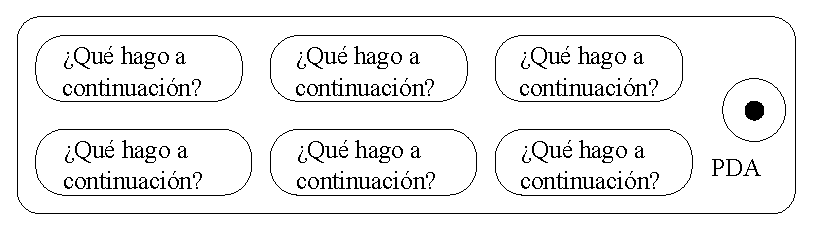
\includegraphics[height=1.00in]{figs2/pda.eps}}
\afterfig

Los programadores añaden un sistema operativo y un conjunto de
aplicaciones al hardware y así tenemos al final un Asistente Personal
Digital que resulta bastante útil y capaz de ayudarnos a hacer
muchas cosas diferentes.

Nuestros ordenadores son rápidos, tienen gran cantidad de memoria
y podrían resultarnos muy útiles si tan solo conociéramos el idioma
que debemos hablar para explicar al ordenador qué queremos que
``haga a continuación''. Si conociéramos ese idioma, podríamos pedirle al
ordenador que realizase tareas repetitivas para nosotros. 
Precisamente, el tipo de cosas que los ordenadores hacen mejor
suelen ser el tipo de cosas que los humanos encuentran aburridas
y soporíferas.

Por ejemplo, echa un vistazo a los primeros tres párrafos de este
capítulo y dime cual es la palabra más utilizada y cuántas veces
se ha usado. A pesar de que seas capaz de leer y comprender
las palabras en unos pocos segundos, contarlas cuesta más,
porque no es el tipo de problema que las mentes humanas
fueron diseñadas para resolver. Para un ordenador
es justo al revés: leer y comprender texto
de un trozo de papel es algo complicado para él,
pero contar las palabras y decir cuántas veces
se ha usado la más frecuente le resulta muy sencillo:

\beforeverb
\begin{verbatim}
python words.py
Introduce fichero:words.txt
que 8
\end{verbatim}
\afterverb
%
Nuestro ``asistente analista de información personal'' nos dirá
rápidamente que la palabra ``que'' se ha usado ocho veces en los
primeros tres párrafos de este capítulo.

El hecho de que los ordenadores sean buenos en cosas
en las que los humanos no lo son es el motivo por el que necesitas
ser capaz de hablar ``idioma de ordenador''. Una vez que hayas
aprendido ese nuevo idioma, podrás delegar tareas mundanas
en tu socio (el ordenador), dejando más tiempo libre
para ti, de modo que puedas dedicarte a aquellas otras cosas
para las que estás más capacitado. Serás el encargado
de poner la creatividad, intuición e inventiva a esa
asociación.

\section{Creatividad y motivación}

Aunque este libro no está dirigido a programadores profesionales, la programación
profesional puede ser un trabajo muy gratificante tanto a nivel financiero como personal.
Construir programas útiles, elegantes e ingeniosos para que otros los usen
es una actividad muy creativa. Tu ordenador o Asistente Personal Digital (PDA),
normalmente contienen muchos programas diferentes de multitud de grupos de programadores
distintos, cada uno de los cuales compite por tu atención e interés.
Esos programadores intentan hacerlo lo mejor que saben para adaptarse a tus necesidades y
proporcionarte una buena experiencia de usuario en tu tarea. En algunos casos, cuando eliges un
programa determinado, los programadores son directamente recompensados por tu elección.

Si pensamos en los programas como salida creativa para grupos de programadores,
tal vez la siguiente figura sea una versión más acertada de tu PDA:

\beforefig
\centerline{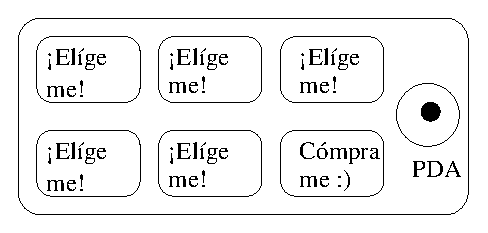
\includegraphics[height=1.00in]{figs2/pda2.eps}}
\afterfig

Por ahora, nuestra motivación principal no es conseguir dinero o gustar más a los usuarios
finales, sino ser más productivos para nosotros mismos en el manejo de los datos e
información que encontraremos en nuestras vidas.
Al principio, serás tanto programador como usuario final de tus propios programas.
Cuando ganes en habilidad como programador y la programación se haga más creativa para ti,
tus ideas podrán avanzar desarrollando programas para otros.

\section{Arquitectura hardware del ordenador}
\index{hardware}
\index{hardware!arquitectura}

Antes de que empecemos a aprender el idioma que deberemos hablar
para dar instrucciones a los ordenadores o desarrollar
software, necesitamos aprender un poco acerca de cómo
están construidos los ordenadores. Si desmontaras
tu ordenador o teléfono móvil y mirases dentro,
encontrarías los siguientes componentes:

\beforefig
\centerline{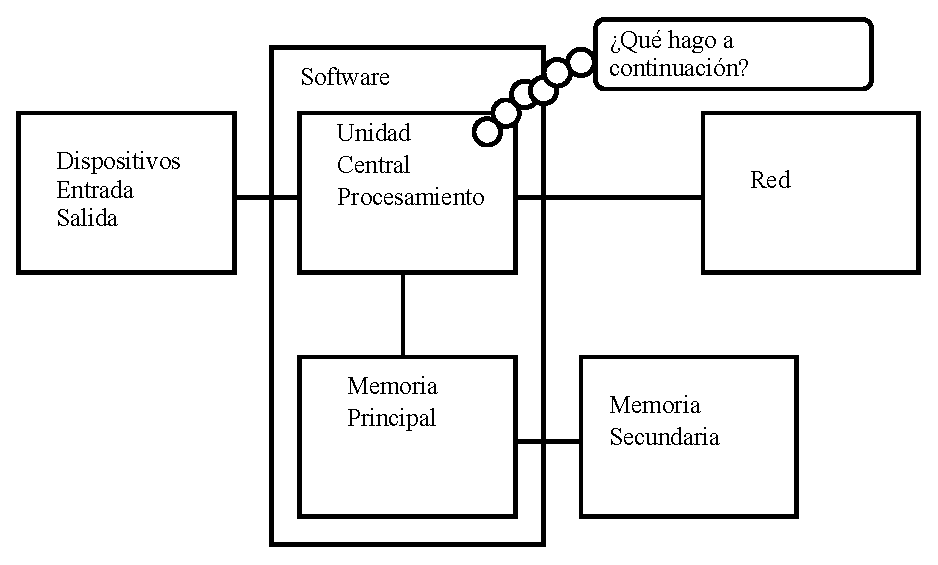
\includegraphics[height=2.50in]{figs2/arch.eps}}
\afterfig

Las definiciones de alto-nivel de estos componentes son las siguientes:

\begin{itemize}

\item La {\bf Unidad Central de Procesamiento} (o CPU) es
la parte del ordenador que está construida para estar obsesionada
con el ``¿qué es lo siguiente?'' Si tu ordenador está clasificado
como de 3.0 Gigahercios, significa que la CPU va a preguntar ``¿Qué hago a continuación?''
tres mil millones de veces por segundo. Tendrás que aprender a hablarle muy
rápido para mantener el ritmo de esa CPU.

\item La {\bf Memoria Principal} se usa para almacenar la información
que la CPU necesitará enseguida. La memoria principal es casi
tan rápida como la CPU. Pero la información almacenada en la memoria
principal se desvanece cuando el ordenador se apaga.

\item La {\bf Memoria Secundaria} Es también utilizada para almacenar
información, pero es mucho más lenta que la memoria principal.
La ventaja de la memoria secundaria es que puede mantener
almacenada la información incluso cuando el ordenador está apagado.
Ejemplos de memoria secundaria son las unidades de disco o las
memorias flash (que se encuentran normalmente en lápices USB y
reproductores de música portátiles).

\item Los {\bf Dispositivos de Entrada y Salida} son simplemente
la pantalla, teclado, ratón, micrófono, altavoces, touchpad, etc.
Son todos los aparatos que utilizamos para interactuar con el ordenador.

\item En la actualidad, la mayoría de los ordenadores disponen también de una
{\bf Conexión de Red} para recibir información a través de la red.
Podemos pensar en la red como en un sitio muy lento donde se almacenan
y recuperan datos, que puede no estar siempre ``preparado''. Así que en cierto sentido,
la red es una forma lenta y a veces poco fiable de
{\bf Memoria Secundaria}.

\end{itemize}

Aunque la mayoría de los detalles de cómo funcionan estos componentes es mejor
dejarlos para los que construyen ordenadores, resulta útil tener cierta terminología
con la que referirnos a todas estas partes distintas mientras escribimos nuestros programas.

Como programador, tu trabajo es usar y orquestar cada uno de esos
recursos para resolver el problema que necesites solucionar
y analizar los datos que obtengas de la solución. Como programador, principalmente
estarás ``hablando'' con la CPU y diciéndole qué debe hacer a continuación.
A veces le dirás a la CPU que use la memoria principal,
la memoria secundaria o los dispositivos de entrada/salida.

\beforefig
\centerline{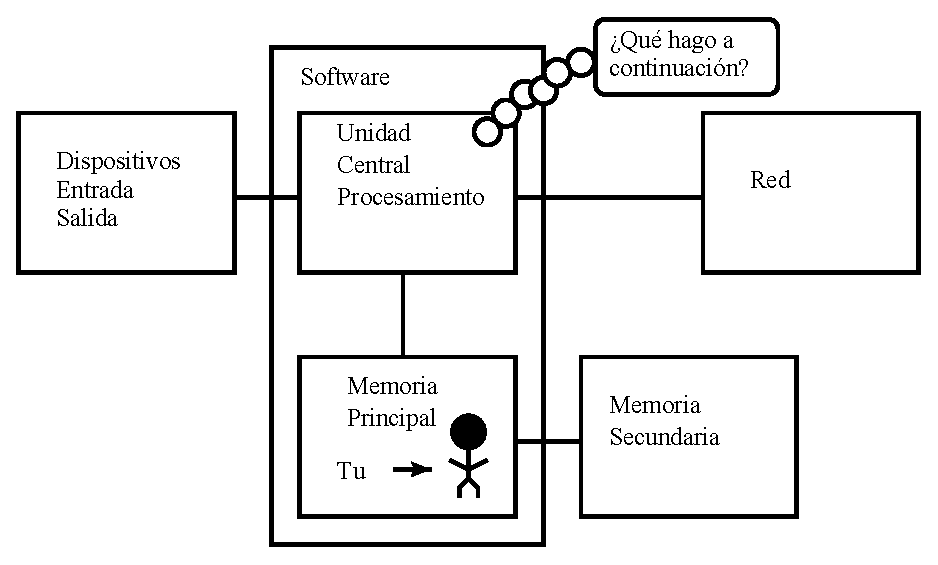
\includegraphics[height=2.50in]{figs2/arch2.eps}}
\afterfig

Tú debes ser la persona que conteste a la pregunta de la CPU ``¿Qué hago a continuación?''.
Pero sería muy incómodo encogerse hasta los 5mm de altura
y meterse dentro del ordenador sólo para poder pasarle un comando
tres mil millones de veces por segundo. Así que en vez de eso,
deberás ponerle por escrito las instrucciones por adelantado.
Llamaremos a esas instrucciones almacenadas un {\bf programa}, y al acto
de escribir las instrucciones y conseguir que
sean correctas, {\bf programar}.

\section{Comprendiendo la programación}

Durante el resto de este libro, intentaremos convertirte en una persona
hábil en el arte de programar. Al final serás un
{\bf programador} --- tal vez no un programador profesional, pero
al menos tendrás la capacidad de echar un vistazo a un problema de análisis
de datos/información y desarrollar un programa para resolverlo.

\index{resolución de problemas}

En cierto sentido, necesitas dos habilidades para ser un programador:

\begin{itemize}

\item En primer lugar, debes dominar el lenguaje de programación (Python) -
debes conocer su vocabulario y su gramática. Debes ser capaz de escribir
las palabras en este nuevo lenguaje correctamente y saber cómo construir
``frases'' bien formadas en este lenguaje.

\item En segundo lugar, debes ``contar una historia''. Al escribir una historia,
combinas palabras y frases para transmitir un concepto al lector.
Son necesarios habilidad y arte para construir la historia, y esa habilidad
se mejora precisamente escribiendo y teniendo cierta retroalimentación.
En programación, nuestro programa es la ``historia'' y el problema
que estás tratando de resolver es el ``concepto''.

\end{itemize}

Una vez que aprendas un lenguaje de programación como Python, encontrarás
mucho más sencillo aprender un segundo lenguaje como JavaScript o C++.
Cada nuevo lenguaje de programación tendrá un vocabulario y gramática muy
diferentes, pero la forma de resolver problemas
va a ser la misma en todos ellos.

Aprenderás el ``vocabulario'' y ``frases'' de Python muy rápidamente.
Te contará un poco más ser capaz de escribir un programa coherente
para resolver un problema nuevo. Se enseña a programar de forma muy similar
a como se enseña a escribir. Se comienza leyendo y explicando programas,
después se escriben programas simples, y se va incrementando la complejidad
de ellos poco a poco. En algún momento ``encuentras tu musa'' y comienzas
a descubrir los patrones por ti mismo, de modo que ya eres capaz de tomar un
problema y escribir un programa para resolverlo. Y una vez has llegado a ese
punto, la programación se convierte en un proceso muy agradable y creativo.

Comenzaremos con el vocabulario y estructura de los programas en Python. Ten
paciencia si la simplicidad de los ejemplos te recuerdan a cuando empezaste
a leer por primera vez.

\section{Palabras y frases}
 \index{programación, lenguaje}
 \index{lenguaje!programación}

A diferencia de los idiomas humanos, el vocabulario de Python es actualmente
bastante reducido. Llamamos a ese ``vocabulario'' las ``palabras reservadas''.
Son palabras que tienen un significado muy especial para Python. Cuando Python
encuentra esas palabras en un programa, tienen un significado y sólo uno para Python.
Más adelante, cuando escribas programas, compondrás tus propias palabras, que tendrán significado para ti, llamadas {\bf variables}. Tendrás una gran libertad para escoger los nombres para tus variables, pero no podrás usar ninguna de las palabras reservadas de Python.

Cuando se entrena a un perro, se usan palabras especiales como
``siéntate'', ``quieto'', y ``traelo''. Cuando hablas con un perro y
no usas ninguna de las palabras reservadas, sólo consigues que te mire
con cara extraña hasta que le digas una palabra reservada.
Por ejemplo, si le dices:
``Me gustaría que hubiera más gente que se dedicase a pasear para mejorar su salud'',
lo que la mayoría de los perros oirían sería:
``bla bla bla {\bf pasear} bla bla bla bla.''.
Esto se debe a que ``pasear'' es una palabra reservada en el idioma del perro.
Mucha gente sugeriría que el idioma entre humanos y gatos no tiene
palabras reservadas\footnote{\url{http://xkcd.com/231/}}.

Las palabras reservadas en el idioma en que los humanos hablan con
Python contiene las siguientes:

\beforeverb
\begin{verbatim}
and       del       from      not       while    
as        elif      global    or        with     
assert    else      if        pass      yield    
break     except    import    print              
class     exec      in        raise              
continue  finally   is        return             
def       for       lambda    try
\end{verbatim}
\afterverb
%
Eso es todo, y a diferencia de un perro, Python ya está completamente entrenado.
Cuando utilices ``try'', Python lo intentará cada vez que se lo digas sin
equivocarse\footnote{``try'' en inglés puede traducirse como ``intento''(Nota del Trad.)}.

Aprenderemos esas palabras reservadas y cómo usarlas a su debido tiempo,
pero por ahora nos centraremos en la equivalencia en Python de ``habla''
(en el idioma humano-a-perro). Lo bueno de pedirle a Python que hable
es que podemos incluso decirle qué debe decir, pasándole un mensaje entre comillas:

\beforeverb
\begin{verbatim}
print '¡Hola, mundo!'
\end{verbatim}
\afterverb

Y ya hemos escrito nuestra primera frase sintácticamente correcta en Python.
Nuestra sentencia comienza con la palabra reservada {\bf print}, seguida
por una cadena de texto de nuestra elección, encerrada entre comillas simples.

\section{Conversando con Python}

Ahora que ya conocemos una palabra y una sentencia simple en Python,
debemos aprender cómo comenzar una conversación con Python para probar
nuestras nuevas habilidades.

Antes de que puedas conversar con Python, debes instalar en primer lugar
el software de Python en tu ordenador, y aprender a ponerlo en marcha.
La explicación sobre cómo conseguirlo excede el propósito de este capítulo,
así que te sugiero consultar \url{www.pythonlearn.com}, donde tengo
instrucciones detalladas y capturas de pantallas sobre cómo instalar y poner en marcha
Python en sistemas Macintosh y Windows\footnote{En los capítulos finales del libro también
encontrarás dos apéndices con instrucciones sobre la instalación de Python en esos sistemas (Nota
del trad.)}. En algún momento, terminarás en un terminal
o ventana de comandos, escribirás {\bf python}, y el intérprete de Pyhton
comenzará a ejecutarse en modo interactivo, apareciendo algo como lo siguiente:

\index{interactivo, modo}

\beforeverb
\begin{verbatim}
Python 2.6.1 (r261:67515, Jun 24 2010, 21:47:49) 
[GCC 4.2.1 (Apple Inc. build 5646)] on darwin
Type "help", "copyright", "credits" or "license" for more information.
>>> 
\end{verbatim}
\afterverb
%
El prompt o indicador {\tt \verb">>>"} es el modo que tiene el intérprete de Python de preguntarte:
``¿Qué quieres que haga a continuación?''. Python está preparado para tener una conversación contigo. Todo lo que tienes que hacer es hablar el idioma de Python.

Imaginemos por ejemplo que no conoces ni siquiera la más simple de las palabras o frases del lenguaje Python. Tal vez quieras usar la línea habitual que siguen los astronautas cuando aterrizan en un planeta remoto y quieren hablar con sus habitantes:

\beforeverb
\begin{verbatim}
>>> Venimos en son de paz, por favor llevadnos ante vuestro lider
  File "<stdin>", line 1
    Venimos en son de paz, por favor llevadnos ante vuestro lider
         ^
SyntaxError: invalid syntax
>>> 
\end{verbatim}
\afterverb
%
Esto no está funcionando. A menos que pienses en algo rápido,
los habitantes del planeta probablemente te clavarán sus lanzas,
te ensartarán en un asador, te cocinarán sobre el fuego, y te usarán como cena.

Por suerte has comprado una copia de este libro durante el viaje, así que lo hojeas
hasta llegar precisamente a esta página y pruebas de nuevo:

\beforeverb
\begin{verbatim}
>>> print '¡Hola, mundo!'
¡Hola, mundo!
\end{verbatim}
\afterverb
%
Esto tiene mejor aspecto, así que intentas comunicarte un poco
más:

\beforeverb
\begin{verbatim}
>>> print 'Tú debes ser el dios legendario que viene del cielo'
Tú debes ser el dios legendario que viene del cielo
>>> print 'Hemos estado esperándote durante mucho tiempo'
Hemos estado esperándote durante mucho tiempo
>>> print 'Nuestras leyendas dicen que debes estar muy sabroso con mostaza'
Nuestras leyendas dicen que debes estar muy sabroso con mostaza
>>> print 'Vamos a tener un festín esta noche a menos que digas
  File "<stdin>", line 1
    print 'Vamos a tener un festín esta noche a menos que digas
                                                              ^
SyntaxError: EOL while scanning string literal
>>> 
\end{verbatim}
\afterverb
%
La conversación fue bien durante un rato, y entonces, en cuanto
cometiste un pequeño error usando el lenguaje Python, Python
volvió a apuntarte con las lanzas.

En este momento, ya deberías haberte dado cuenta de que, a pesar de que Python
es increíblemente complejo, potente y muy exigente con
la sintaxis que debes usar para comunicarte con él, Python {\em no} es
inteligente. En realidad tan sólo estás teniendo una conversación
contigo mismo, eso sí, usando una sintaxis correcta.

En cierto sentido, cuando usas un programa escrito por otra persona,
la conversación se mantiene entre tú mismo y esos otros programadores,
con Python actuando como intermediario. Python es un
modo de que los creadores de programas puedan expresar cómo creen
que deben desarrollarse las conversaciones. Y dentro
de unos pocos capítulos más, tú serás uno de esos programadores
que usan Python para hablar con los usuarios de sus programas.

Antes de terminar nuestra primera conversación con el intérprete
de Python, probablemente debas saber cual es el modo correcto
de decir ``adios'' cuando estás interactuando con los
habitantes del Planeta Python:

\beforeverb
\begin{verbatim}
>>> adios
Traceback (most recent call last):
  File "<stdin>", line 1, in <module>
NameError: name 'adios' is not defined

>>> if you don't mind, I need to leave
  File "<stdin>", line 1
    if you don't mind, I need to leave
             ^
SyntaxError: invalid syntax

>>> quit()
\end{verbatim}
\afterverb
%
Te habrás dado cuenta de que el error es diferente en los primeros
dos intentos, a pesar de ser ambos incorrectos. El segundo error es diferente porque
{\bf if} es una palabra reservada, y Python vió la palabra
reservada en la frase y creyó que estabas intentando decirle algo, pero encontró
la sintaxis de la sentencia incorrecta.

El modo correcto de decir ``adios'' a Python es introducir
{\bf quit()} en el indicador interactivo {\tt \verb">>>"}.
Probablemente te hubiera llevado un buen rato adivinarlo,
así que es posible que tener un libro a mano
esté empezando a resultarte útil.

\section{Terminología: intérprete y compilador}

Python es un lenguaje de {\bf alto nivel}, que intenta ser relativamente
sencillo de escribir y leer para los humanos y fácil de leer y procesar para
los ordenadores. Hay otros lenguajes de alto nivel, como Java, C++,
PHP, Ruby, Basic, Perl, JavaScript, y muchos más. El hardware que está
actualmente dentro del la Unidad Central de Procesamiento (CPU) no comprende
ninguno de estos lenguajes de alto nivel.

La CPU comprende un lenguaje que se llama {\bf código máquina}. El código
máquina es muy simple y francamente muy cansado de escribir, porque
en él todo está representado por ceros y unos:

\beforeverb
\begin{verbatim}
01010001110100100101010000001111
11100110000011101010010101101101
...
\end{verbatim}
\afterverb
%
El código máquina superficialmente parece muy sencillo, dado que sólo hay
ceros y unos, pero su sintaxis es incluso más complicada
y mucho más intrincada que Python. Así que muy pocos programadores
usan este lenguaje. En vez de eso, se han construido varios traductores para
permitir a los programadores escribir en lenguajes de alto nivel, como Python
o JavaScript, y esos traductores convierten luego los programas a código máquina
para que la CPU pueda ejecutarlos.

Dado que el código máquina está ligado al hardware del ordenador, ese código
no es {\bf portable} a través de los diferentes tipos de hardware. Los programas escritos
en lenguajes de alto nivel pueden ser trasladados entre ordenadores diferentes usando
un intérprete diferente en la nueva máquina o recompilando el código para crear
una versión en código máquina del programa para el nuevo equipo.

Estos traductores de lenguajes de programación se clasifican en dos categorías generales:
(1) intérpretes y (2) compiladores.

Un {\bf intérprete} lee el código fuente del programa tal y como lo ha escrito
el programador, analiza ese código fuente e interpreta las instrucciones al vuelo.
Python es un intérprete y cuando estamos haciéndolo funcionar de forma interactiva,
podemos escribir una línea de Python (una sentencia), y Python la procesa inmediatamente
y queda listo para que podemos escribir otra nueva línea.

Algunas de las líneas de Python le indican que lo que queremos es recordar cierto
valor para más tarde. Debemos elegir un nombre para que ese valor sea recordado y
podremos usar ese nombre simbólico para recuperar el valor después. Usamos el
término {\bf variable} para referirnos a las etiquetas que utilizamos para manejar esos
datos almacenados.

\beforeverb
\begin{verbatim}
>>> x = 6
>>> print x
6
>>> y = x * 7
>>> print y
42
>>> 
\end{verbatim}
\afterverb
%
En este ejemplo, le pedimos a Python que recuerde el valor seis y use la etiqueta {\bf x},
para que podemos recuperar ese valor más tarde. Comprobamos que Python ha guardado de
momento el valor usando {\bf print}. A continuación le pedimos a Python que recupere {\bf x}, lo multiplique por siete y coloque el nuevo valor calculado en {\bf y}. Finalmente, le pedimos a Python que imprima el valor que está actualmente en {\bf y}.

Aunque estemos escribiendo estos comandos en Python línea por línea, Python
los está tratando como una secuencia ordenada de declaraciones, de modo
que las últimas declaraciones son capaces de recuperar datos creados en las
anteriores. Estamos escribiendo nuestro primer párrafo simple con cuatro frases
en un orden lógico y útil.

La naturaleza de un {\bf intérprete} es ser capaz de tener una conversación interactiva como se muestra más arriba. Un {\bf compilador} necesita que le entreguen el programa
completo en un archivo, y después
ejecuta un proceso para trasladar el código fuente de alto nivel a código máquina.
A continuación el compilador guarda el código máquina resultante en un archivo para su
posterior ejecución. 

Si usas un sistema Windows, a menudo esos programas ejecutables en código máquina tienen un sufijo como ``.exe'' or ``.dll'', que indican ``executable (ejecutable)'' y ``dynamic
link library (librería de enlace dinámico)'' respectivamente. En Linux y Macintosh
no hay un sufijo que marque de forma única un archivo como ejecutable.

Si abrieras un archivo ejecutable en un editor de texto, se mostraría algo
completamente disparatado e ilegible:

\beforeverb
\begin{verbatim}
^?ELF^A^A^A^@^@^@^@^@^@^@^@^@^B^@^C^@^A^@^@^@\xa0\x82
^D^H4^@^@^@\x90^]^@^@^@^@^@^@4^@ ^@^G^@(^@$^@!^@^F^@
^@^@4^@^@^@4\x80^D^H4\x80^D^H\xe0^@^@^@\xe0^@^@^@^E
^@^@^@^D^@^@^@^C^@^@^@^T^A^@^@^T\x81^D^H^T\x81^D^H^S
^@^@^@^S^@^@^@^D^@^@^@^A^@^@^@^A\^D^HQVhT\x83^D^H\xe8
....
\end{verbatim}
\afterverb
%
No es fácil leer o escribir código máquina, así que está bien que tengamos
{\bf intérpretes} y {\bf compiladores} que nos permitan escribir en lenguajes
de alto nivel, como Python o C.

En este momento de la discusión acerca de compiladores e intérpretes, deberías
estar preguntándote algunas cosas sobre el mismo intérprete de Python. ¿En qué
lenguaje ha sido escrito? ¿Ha sido escrito en un lenguaje compilado? Cuando escribimos ``python'', ¿qué es exactamente lo que ocurre?

El intérprete de Python está escrito en un lenguaje de alto nivel llamado ``C''.
Puedes ver el código fuente real del intérprete de Python acudiendo a
\url{www.python.org}, y hacer lo que quieras con su código fuente.
Así que el propio Python es también un programa, y está compilado en código máquina.
Cuando instalaste Python en tu ordenador (o el vendedor lo instaló),
pusiste una copia del código máquina del programa Python traducido para tu sistema.
En Windows, el ejecutable en código máquina del propio Python es probablemente
un archivo con un nombre como:

\beforeverb
\begin{verbatim}
C:\Python27\python.exe
\end{verbatim}
\afterverb
%
Esto ya es más de lo que en realidad necesitas saber para ser un programador en Python,
pero a veces es mejor responder a estas típicas preguntillas justo
al principio.

\section{Escribir un programa}

Escribir frases en el intérprete de Python es un buen modo de experimentar
con las características de Python, pero no se recomienda para resolver problemas
de cierta complejidad.

Cuando queremos escribir un programa,
usamos un editor de texto para escribir las instrucciones de Python en un archivo,
que se denomina un {\bf script}. Por
convención, los scripts en Python tienen nombres que terminan en {\tt .py}.

\index{script}

Para ejecutar un script, tienes que indicarle al intérprete de Python
el nombre del archivo. En una ventana de comandos de Unix o Windows,
puedes escribir {\tt python hello.py} así:

\beforeverb
\begin{verbatim}
csev$ cat hello.py
print '¡Hola, mundo!'
csev$ python hello.py
¡Hola, mundo!
csev$
\end{verbatim}
\afterverb
%
El ``csev\$'' es el indicador del sistema operativo, y el ``cat hello.py'' nos
está mostrando que el archivo ``hello.py'' contiene un programa Python de una línea
que imprime una cadena.

Estamos llamando al intérprete de Pyhton e indicándole que lea el código fuente del
archivo ``hello.py'', en vez de ir escribiendo nosotros las líneas de código Python
de forma interactiva.

Habrás notado que no es necesario poner {\bf quit()} al final del programa
Python en el archivo. Cuando Python está leyendo el código fuente
desde un archivo, sabe parar cuando llega al final del fichero.

\section{¿Qué es un programa?}

La definición más básica de un {\bf programa} es que se trata de una
secuencia de sentencias de Python que han sido creadas para hacer algo.
Incluso nuestro simple script {\bf hello.py} es un programa. Es un programa
de una sola línea y no particularmente útil, pero en su más estricta definición,
es un programa Python. 

Debería ser más sencillo comprender qué es un programa si pensásemos en un problema
que pudiera resolverse mediante programación, y a continuación estudiásemos cómo sería el
programa que resolviera ese problema.

Imaginemos que estás haciendo una investigación sobre estadística social en los mensajes
de Facebook, y estás interesado en saber cuál es la palabra que se usa con mayor frecuencia
en una serie de mensajes. Podrías imprimir la cadena de mensajes de Facebook y estudiar
detenidamente el texto, buscando la palabra más común, pero eso te llevaría mucho tiempo
y lo más probable sería que cometieses errores. Sería más inteligente escribir un programa
en Python para realizar la tarea rápidamente y con precisión, y así podrías emplear el fin
de semana en hacer algo divertido.

Por ejemplo, mira el texto siguiente acerca de un payaso y un coche. Fijate en el
texto y busca cual es la palabra más común y cuántas veces se repite.

\beforeverb
\begin{verbatim}
el payaso corrió detrás del coche y el coche se metió en la carpa
y la carpa se cayó sobre el payaso y el coche
\end{verbatim}
\afterverb
%
Después imagina que estás haciendo esta tarea buscando en millones de líneas de
texto. Francamente, te resultaría más rápido aprender Python y escribir un
programa para contar las palabras que revisarlas manualmente una a una.

La buena noticia es que a mí ya se me ha ocurrido un programa
simple para encontrar la palabra más común en un archivo de texto. Lo he escrito,
probado, y ahora te lo doy a ti para que lo uses y puedas ahorrarte algo de tiempo.

\beforeverb
\begin{verbatim}
name = raw_input('Introduce archivo:')
manejador = open(nombre, 'r')
texto = manejador.read()
palabras = texto.split()
contadores = dict()

for palabra in palabras:
   contadores[palabra] = contadores.get(palabra,0) + 1

mayorcantidad = None
mayorpalabra = None
for palabra,contador in contadores.items():
    if mayorcantidad is None or contador > mayorcantidad:
        mayorpalabra = palabra
        mayorcantidad = contador

print mayorpalabra, mayorcantidad
\end{verbatim}
\afterverb
%
No necesitas ni siquiera saber Python para utilizar este programa. Deberás llegar hasta
el capítulo 10 de este libro para comprender del todo las impresionantes técnicas que
se han usado para crear este programa. Eres el usuario final, simplemente utiliza el
programa y maravíllate de su ingenio y de cuánto esfuerzo manual te ha ahorrado.
Simplemente escribe el código
en un archivo llamado {\bf words.py} y ejecútalo, o descarga el código fuente
de \url{http://www.pythonlearn.com/code/} y hazlo funcionar.

\index{programa}
Este es un buen ejemplo de cómo Python y el lenguaje Python están actuando de
intermediarios entre tú (el usuario final) y yo (el programador). Python es para nosotros
un modo de intercambiar secuencias de instrucciones útiles (p.e. programas) en un
lenguaje común que puede ser usado por cualquiera que instale
Python en su ordenador. Así que ninguno de nosotros estamos hablando {\em a Python},
sino que estamos comunicándonos mutuamente {\em a través de} Python.

\section{Los bloques de construcción de los programas}

En los próximos capítulos, aprenderemos más acerca del vocabulario, estructura de las
frases, estructura de los párrafos, y estructura de las historias de Python. Aprenderemos
sobre las potentes capacidades de Python y cómo usar esas capacidades juntas para crear
programas útiles.

Hay ciertos modelos conceptuales de bajo nivel que se usan para construir programas.
Estas estructuras no son exclusivas de los programas Python, sino que son parte de
cualquier lenguaje de programación, desde el código máquina hasta los lenguajes de alto
nivel.

\begin{description}

\item[entrada:] Obtiene datos del ``mundo exterior''. Puede consistir en
leer datos de un archivo, o incluso de algún tipo de sensor, como un micrófono
o GPS. En nuestros programas iniciales la entrada vendrá del propio usuario,
escribiendo datos en el teclado.

\item[salida:] Muestra el resultado del programa en la pantalla
o lo almacena en un archivo; o tal vez lo escribe en un dispositivo, como puede ser
un altavoz, para reproducir música o leer texto.

\item[ejecución secuencial:] Ejecuta sentencias una detrás de otra,
en el orden en que se encuentran en el script.

\item[ejecución condicional:] Comprueba ciertas condiciones y
después ejecuta u omite una secuencia de sentencias.

\item[ejecución repetida:] Ejecuta cierto conjunto de sentencias
repetidamente, normalmente con alguna variación.

\item[reutilización:] Se escriben un conjunto de instrucciones una vez y se las da un nombre
para después reutilizarlas cuando sean necesarias en cualquier otra parte
del programa.

\end{description}

Parece demasiado simple para ser verdad, y por supuesto nunca es tan simple.
Es como decir que caminar es simplemente
``poner un pie delante del otro''. El ``arte''
de escribir un programa es componer y entrelazar juntos estos
elementos básicos muchas veces, para producir algo
que sea útil a sus usuarios.

El programa anterior que calcula el número de palabras usa directamente
todos estos patrones, excepto uno.

\section{¿Qué es posible que vaya mal?}

Como hemos visto en nuestra primera conversación con Python, deberemos
comunicarnos de forma muy precisa cuando escribamos código Python. La mínima
desviación o error provocará que Python deje de ejecutar
nuestro programa.

Los programadores novatos a menudo se toman el hecho de que Python no
deje espacio para errores como una prueba de que Python es perverso, odioso y cruel.
Aunque a Python parece que le gustan todos los demás, reconoce a los novatos
y les guarda rencor. Debido a ese rencor,
Python toma sus programas perfectamente escritos y los rechaza como si fueran
``inútiles'' sólo para atormentarnos.

\beforeverb
\begin{verbatim}
>>> primt '¡Hola, mundo!'
  File "<stdin>", line 1
    primt '¡Hola, mundo!'
                       ^
SyntaxError: invalid syntax
>>> primt 'Hola, mundo'
  File "<stdin>", line 1
    primt 'Hola, mundo'
                      ^
SyntaxError: invalid syntax
>>> ¡Te odio, Python!
  File "<stdin>", line 1
    ¡Te odio, Python!
         ^
SyntaxError: invalid syntax
>>> si sales fuera, te daré una lección
  File "<stdin>", line 1
    si sales fuera, te daré una lección
              ^
SyntaxError: invalid syntax
>>> 
\end{verbatim}
\afterverb
%
Hay poco que ganar discutiendo con Python. Sólo es una herramienta.
No tiene emociones, es feliz y está listo para servirte en cualquier momento
que le necesites. Sus mensajes de error parecen crueles, pero son simples
peticiones de ayuda de Python. Ha examinado lo que has escrito y simplemente
no es capaz de entender lo que has puesto.

Python se parece mucho a un perro: te quiere incondicionalmente, pero sólo es capaz
de entender unas pocas palabras clave, así que te mira con una expresión
adorable en su cara ({\tt \verb">>>"}),y espera a que tú le digas algo que él pueda comprender.
Cuando Python dice ``SyntaxError: invalid syntax'', está simplemente agitando
su cola y diciendo: ``Me parece que has dicho algo, pero es que no comprendo
lo que significa. De todos modos, sigue hablando conmigo, por favor ({\tt \verb">>>"}).''

Cuando tus programas vayan aumentando su complejidad, te encontrarás con
tres tipos de errores en general:

\begin{description}

\item[Errores de sintaxis:] Estos son los primeros errores que cometerás y los más
fáciles de corregir. Un error de sintaxis quiere decir que has violado las reglas de la
``gramática'' de Python. Python hace lo que puede para indicar la línea y el carácter
correctos en donde ha cree que está la confusión. Lo único complicado de los errores de
sintaxis es que a veces el error que se necesita corregir está en alguna línea del
programa anterior a aquella en la cual Python emite el {\em aviso}. De modo que la línea
y el carácter que Python indica en un error de sintaxis pueden ser sólo un punto de
partida para tu investigación.  

\item[Errores lógicos:] Un error lógico es cuando tu programa tiene una sintaxis correcta,
pero existe un error en el orden de las sentencias o tal vez un error en cómo las
sentencias se relacionan unas con otras.
Un buen ejemplo de un error lógico sería, ``toma un trago de tu botella de agua, ponla
en tu mochila, camina hasta la biblioteca, y luego vuelve a poner el tapón a la botella.'' 

\item[Errores semánticos:] Un error semántico se produce cuando la descripción de los
pasos a seguir es sintácticamente perfecta y se realiza en el orden correcto, pero
simplemente existe un error en el programa. El programa es perfectamente correcto, pero
no realiza aquello que tú {\em pretendías} que hiciera. Un ejemplo sencillo podría ser
si tú estuvieses indicando a alguien el camino hacia un restaurante y dijeras:
``...cuando llegues a la intersección con la gasolinera, gira a la izquierda, continúa
durante kilómetro y medio y el edificio rojo de tu derecha será el restaurante.'' Tu amigo
se retrasará y te llamará para decirte que está en una granja, y dando vueltas alrededor
de un granero, sin que haya señal alguna de un restaurante.
Entonces le preguntarás: ``¿Giraste a la izquierda o a la derecha en la gasolinera?'', y él
responderá: ``Seguí al pie de la letra tus indicaciones, las tengo por escrito, y decían
que debía girar la izquierda y continuar kilómetro y medio desde la gasolinera.'' Entonces
le dirás: ``Lo siento mucho, porque aunque mis instrucciones son sintácticamente
correctas, por desgracia contienen un pequeño e indetectado error semántico.''.

\end{description}

Cuando se produce cualquiera de los tres tipos de errores, Python de nuevo está
simplemente intentando por todos los medios hacer exactamente lo que tú le has pedido.

\section{El viaje de aprendizaje}

Según vayas avanzando por el resto del libro, no te asustes si los conceptos
no parecen encajar bien unos con otros al principio. Cuando estabas aprendiendo a hablar,
no supuso un problema que durante los primeros años sólo pudieras emitir lindos
balbuceos. Y también fue normal que te llevara seis meses pasar de un vocabulario simple
a frases simples y que te llevara 5-6 años más pasar de frases a párrafos, y unos cuantos
años más hasta que fuiste capaz de escribir una historia corta interesante por ti mismo.

Pretendemos que aprendas Python mucho más rápidamente, y todo al mismo tiempo
durante los próximos capítulos.
Aún así, ten en cuenta que esto es como un aprender un idioma nuevo, que lleva un tiempo
absorber y comprender antes de que te resulte familiar.
Eso produce cierta confusión, ya que visitaremos y volveremos a visitar
temas para intentar que consigas ver el conjunto del cuadro mientras vamos definiendo
los pequeños fragmentos que forman esa obra completa. A pesar de que el libro está
escrito de forma lineal, y que si estás participando en un curso éste también avanzará
de forma lineal, no dudes en ser no lineal en el modo en que te aproximes al material.
Avanza y retrocede y lee a veces por encima. Al ojear material más avanzado sin comprender del
todo los detalles tendrás una mejor comprensión del ``¿por qué?'' de la programación.
Al revisar el material anterior e incluso al rehacer los ejercicios previos,
te darás cuenta que ya has aprendido un montón de materia, incluso si la materia
sobre la que estás trabajando en ese momento parece un poco impenetrable.

Normalmente, cuando uno aprende su primer lenguaje de programación, hay unos pocos
momentos estupendos ``¡A-já!'', en los cuales puedes levantar la vista de la roca que
estás machacando con martillo y cincel, separarte unos pasos y comprobar
que lo que estás intentando construir es una maravillosa escultura.

Si algo parece particularmente difícil, generalmente no vale la pena quedarse mirándolo
toda la noche. Tómate un respiro, échate una siesta, come algo, explícale a alguien
(quizás a tu perro) con qué estás teniendo problemas, y después vuelve a ello con nuevos
ojos. Te aseguro que una vez que aprendas los conceptos de la programación en
el libro, volverás atrás y verás que en realidad todo era fácil y elegante y que
simplemente te ha llevado un poco de tiempo llegar a absorberlo.

\section{Glosario}

\begin{description}

\item[bug:] Un error en un programa.
\index{bug}

\item[código fuente:] Un programa en un lenguaje de alto nivel.
\index{código fuente}

\item[código máquina:] El lenguaje de más bajo nivel para el software, ya que se trata
del lenguaje que es directamente ejecutado por la unidad central de procesamiento
(CPU).
\index{código máquina}

\item[compilar:] Traducir un programa escrito en un lenguaje de alto nivel
a otro lenguaje de bajo nivel de una vez, preparándolo para su posterior
ejecución.
\index{compilar}

\item[error semántico:] Un error en un programa que provoca que haga algo
distinto de lo que el programador pretendía.
\index{error!semántico}

\item[interpretar:]  Ejecutar un programa en un lenguaje de alto nivel
traduciendo sus líneas de una en una.
\index{interpretar}

\item[lenguaje de alto nivel:]  Un lenguaje de programación como Python, que
está diseñado para ser sencillo de leer y escribir para los humanos.
\index{lenguaje!de alto nivel}

\item[lenguaje de bajo nivel:]  Un lenguaje de programación que ha sido diseñado
para ser sencillo de ejecutar para un ordenador; también se le llama ``código máquina''
o ``lenguaje ensamblador''.
\index{lenguaje!de bajo nivel}

\item[memoria principal:] Almacena programas y datos. La memoria principal pierde
su información cuando se interrumpe la energía que la alimenta.
\index{memoria!principal}

\item[memoria secundaria:] Almacena programas y datos y retienen su
información incluso cuando la corriente se interrumpe. Generalmente es más lenta
que la memoria principal. Ejemplos de memoria secundaria pueden ser unidades de
disco y memorias flash en lápices USB.
\index{memoria!secundaria}

\item[modo interactivo:] Un modo de uso de usar el intérprete de Python
escribiendo comandos y expresiones en el prompt (indicador).
\index{modo interactivo}

\item[parsear:] Examinar un programa y analizar su estructura sintáctica.
\index{parsear}
\index{analizar}

\item[portabilidad:]  La propiedad de un programa que le permite funcionar en más
de un tipo de ordenador.
\index{portabilidad}

\item[programa:] Un conjunto de instrucciones que especifican un cálculo.
\index{programa}

\item[prompt:] Cuando un programa muestra un mensaje y se detiene para que
el usuario escriba alguna entrada para el programa.
\index{prompt}

\item[resolución de problemas:]  El proceso de formular un problema, encontrar
una solución y expresar la solución.
\index{resolución de problemas}

\item[semántica:] El significado de un programa.
\index{semántica}

\item[sentencia print:]  Una instrucción que provoca que el intérprete de Python
muestre un valor en la pantalla.
\index{print, sentencia}
\index{sentencia!print}

\item[unidad central de procesamiento:] El corazón de cualquier ordenador. Es lo que
ejecuta el software que escribimos; también se le suele llamar ``CPU'' o ``el procesador''.
\index{unidad central de procesamiento}
\index{CPU}

\end{description}

\section{Ejercicios}


\begin{ex}
¿Cuál es la función de la memoria secundaria en un ordenador?

a) Ejecutar todos los cálculos y lógica del programa\\
b) Recuperar páginas web de Internet\\
c) Almacenar información durante mucho tiempo -- incluso entre ciclos de apagado-encendido\\
d) Recoger la entrada del usuario
\end{ex}

\begin{ex}
¿Qué es un programa?
\end{ex}

\begin{ex}
¿Cuál es la diferencia entre un compilador y un intérprete?
\end{ex}

\begin{ex}
¿Cuál de los siguientes contiene ``código máquina''?

a) El intérprete de Python\\
b) El teclado\\
c) El código fuente de Python\\
d) Un documento de un procesador de texto
\end{ex}

\begin{ex}
¿Qué está mal en el código siguiente?:

\beforeverb
\begin{verbatim}
>>> primt '¡Hola, mundo!'
  File "<stdin>", line 1
    primt '¡Hola, mundo!'
                       ^
SyntaxError: invalid syntax
>>> 
\end{verbatim}
\afterverb

\end{ex}

\begin{ex}
¿En qué parte del ordenador queda almacenada una variable como ``X''
después de que termine la siguiente línea de Python?:

\beforeverb
\begin{verbatim}
x = 123
\end{verbatim}
\afterverb
%
a) Unidad Central de Procesamiento\\
b) Memoria Principal\\
c) Memoria Secundaria\\
d) Dispositivos de Entrada\\
e) Dispositivos de Salida
\end{ex}

\begin{ex}
¿Qué imprimirá en pantalla el siguiente programa?:

\beforeverb
\begin{verbatim}
x = 43
x = x + 1
print x
\end{verbatim}
\afterverb
%
a) 43\\
b) 44\\
c) x + 1\\
d) Error, porque x = x + 1 no es posible matemáticamente
\end{ex}

\begin{ex}
Explica cada uno de los siguientes conceptos usando como ejemplo una capacidad humana:
(1) Unidad Central de Procesamiento, (2) Memoria Principal, (3) Memoria Secundaria, 
(4) Dispositivo de Entrada, y
(5) Dispositivo de Salida.
Por ejemplo, ``¿Cuál es el equivalente humano a la Unidad Central de Procesamiento''? 
\end{ex}

\begin{ex}
¿Cómo puedes corregir un ``Error de sintaxis''?
\end{ex}
% LaTeX source for ``Python for Informatics: Exploring Information''
% Copyright (c)  2010-  Charles R. Severance, All Rights Reserved

\chapter{Variables, expresiones y sentencias}

\section{Valores y tipos}
\index{value}
\index{type}
\index{string}

Un {\bf valor} es una de las cosas básicas que utiliza un programa,
como una letra o un número.
Los valores que hemos visto hasta ahora
han sido {\tt 1}, {\tt 2}, y
\verb"'¡Hola, mundo!'"

Esos valores pertenecen a {\bf tipos} diferentes:
{\tt 2} es un entero (int), y \verb"'¡Hola, mundo!'" es una {\bf cadena} (string),
que recibe ese nombre porque contiene una ``cadena'' de letras.
Tú (y el intérprete) podéis identificar
las cadenas porque van encerradas entre comillas.

\index{quotation mark}

La sentencia {\\tt print} funciona también para enteros. Vamos a usar el
comando {\\tt python} para iniciar el intérprete.

\beforeverb
\begin{verbatim}
python
>>> print 4
4
\end{verbatim}
\afterverb
%
Si no estás seguro de qué tipo de valor estás manejando, el intérprete te lo puede decir.

\beforeverb
\begin{verbatim}
>>> type('¡Hola, mundo!')
<type 'str'>
>>> type(17)
<type 'int'>
\end{verbatim}
\afterverb
%
No resulta sorprendente que las cadenas pertenezca al tipo {\tt str}, y los
enteros pertenezcan al tipo {\tt int}. Resulta sin embargo menos obvio
que los números con un punto decimal pertenezcan a un tipo llamado {\\tt float} (flotante),
ya que esos números se representan en un formato
conocido como {\\bf punto flotante}\footnote{En el mundo anglosajón (y también en Python)
la parte decimal de un número se separa de la parte entera mediante un punto, y no mediante una coma
(N. del trad.)}.

\index{type}
\index{string type}
\index{type!str}
\index{int type}
\index{type!int}
\index{float type}
\index{type!float}

\beforeverb
\begin{verbatim}
>>> type(3.2)
<type 'float'>
\end{verbatim}
\afterverb
%
¿Qué ocurre con valores como \verb"'17'" y \verb"'3.2'"?
Parecen números, pero van entre comillas como
las cadenas.

\index{quotation mark}

\beforeverb
\begin{verbatim}
>>> type('17')
<type 'str'>
>>> type('3.2')
<type 'str'>
\end{verbatim}
\afterverb
%
Son cadenas.

Cuando escribes un entero grande, puede que te sientas tentado a usar comas
o puntos para separarlo en grupos de tres dígitos, como en {\tt 1,000,000}
\footnote{En el mundo anglosajón el ``separador de millares'' es la coma, y no el punto (N. del trad.)}.
Eso no es un entero válido en Python, pero en cambio sí que resulta válido algo como:

\beforeverb
\begin{verbatim}
>>> print 1,000,000
1 0 0
\end{verbatim}
\afterverb
%
Bien, ha funcionado. ¡Pero eso no era lo que esperábamos!. Python interpreta
{\\tt 1,000,000} como una secuencia de enteros separados por comas, así que lo
imprime con espacios en medio.

\index{semantic error}
\index{error!semantic}
\index{error message}

Éste es el primer ejemplo que hemos visto de un error semántico: el código
funciona sin producir ningún mensaje de error, pero no hace su trabajo
``correctamente''.

\section{Variables}
\index{variable}
\index{assignment statement}
\index{statement!assignment}

Una de las características más potentes de un lenguaje de programación es
la capacidad para manipular {\bf variables}. Una variable es un nombre
que se refiere a un valor.

Una {\bf sentencia de asignación} crea variables nuevas y las
asigna valores:

\beforeverb
\begin{verbatim}
>>> mensaje = 'Y ahora algo completamente diferente'
>>> n = 17
>>> pi = 3.1415926535897931
\end{verbatim}
\afterverb
%
Este ejemplo hace tres asignaciones. La primera asigna una cadena
a una variable nueva llamada {\\tt mensaje};
la segunda asigna el entero {\\tt 17} a {\tt n}; la tercera
asigna el valor (aproximado) de $\pi$ a {\\tt pi}.

Para mostrar el valor de una variable, se puede usar la sentencia print:

\beforeverb
\begin{verbatim}
>>> print n
17
>>> print pi
3.14159265359
\end{verbatim}
\afterverb
%
El tipo de una variable es el tipo del valor al que se refiere.

\beforeverb
\begin{verbatim}
>>> type(mensaje)
<type 'str'>
>>> type(n)
<type 'int'>
>>> type(pi)
<type 'float'>
\end{verbatim}
\afterverb
%

\section{Nombres de variables y palabras claves}
\index{keyword}

Los programadores generalmente elijen nombres para sus variables que
tengan sentido y documenten para qué se usa esa variable.

Los nombres de las variables pueden ser arbitrariamente largos. Pueden contener
tanto letras como números, pero no pueden comenzar con un número.
Es válido usar letras mayúsculas, pero es buena idea
comenzar los nombres de las variables con una letras minúscula (veremos
por qué después).

El carácter barra-baja (\verb"_") puede utilizarse en un nombre.
A menudo se utiliza en nombres con múltiples palabras, como en
\verb"mi_nombre" or \verb"velocidad_de_golondrina_sin_carga".
Los nombres de las variables pueden comenzar con un carácter barra-baja, pero
generalmente se evita usarlo así a menos que se esté escribiendo código
para librerías que luego usarán otros.

\index{underscore character}

Si se le da a una variable un nombre no permitido, se obtiene un error de sintaxis:

\beforeverb
\begin{verbatim}
>>> 76trombones = 'gran desfile'
SyntaxError: invalid syntax
>>> more@ = 1000000
SyntaxError: invalid syntax
>>> class = 'Teorema avanzado de Zymurgy'
SyntaxError: invalid syntax
\end{verbatim}
\afterverb
%
{\tt 76trombones} es incorrecto porque comienza por un número.
{\tt more@} es incorrecto porque contiene un carácter no premitido, {\\tt @}.
Pero, ¿qué es lo que está mal en {\tt class}?

Pues resulta que {\\tt class} es una de las {\bf palabras clave} de Python. El
intérprete usa palabras clave para reconocer la estructura del programa,
y esas palabras no pueden ser utilizadas como nombres de variables.

\index{keyword}

Python reserva 31 palabras claves\footnote{En Python 3.0, {\tt exec} ya no es
una palabra clave, pero {\tt nonlocal} sí que lo es.} para su propio uso:

\beforeverb
\begin{verbatim}
and       del       from      not       while    
as        elif      global    or        with     
assert    else      if        pass      yield    
break     except    import    print              
class     exec      in        raise              
continue  finally   is        return             
def       for       lambda    try
\end{verbatim}
\afterverb
%
Puede que quieras tener esta lista a mano. Si el intérprete se queja
por el nombre de una de tus variables y no sabes por qué, comprueba
si ese nombre está en esta lisa.

\section{Sentencias}

Una {\bf sentencia} es una unidad de código que el intérprete de Python puede
ejecutar. Hemos visto hasta ahora dos tipos de sentencia: print
y las asignaciones.

\index{statement}
\index{interactive mode}
\index{script mode}

Cuando escribes una sentencia en modo interactivo, el intérprete la
ejecuta y muestra el resultado, si es que lo hay.

Un script normalmente contiene una secuencia de sentencias. Si hay
más de una sentencia, los resultados aparecen de uno en uno
según se van ejecutando las sentencias.

Por ejemplo, el script

\beforeverb
\begin{verbatim}
print 1
x = 2
print x
\end{verbatim}
\afterverb
%
produce la salida

\beforeverb
\begin{verbatim}
1
2
\end{verbatim}
\afterverb
%
La sentencia de asignación no produce ninguna salida.


\section{Operadores y operandos}
\index{operator, arithmetic}
\index{arithmetic operator}
\index{operand}
\index{expression}

{\bf Los operadores} son símbolos especiales que representan cálculos, como
la suma o la multiplicación. Los valores a los cuales se aplican esos operadores
reciben el nombre de {\bf operandos}.

Los operadores {\tt +}, {\tt -}, {\tt *}, {\tt /}, and {\tt **}
realizan sumas, restas, multiplicaciones, divisiones y
exponenciación (elevar un número a una potencia), como se muestra en los siguientes ejemplos:

\beforeverb
\begin{verbatim}
20+32   hora-1   hora*60+minuto   minuto/60   5**2   (5+9)*(15-7)
\end{verbatim}
\afterverb
%
El operador de división puede que no haga exactamente lo que esperas:

\beforeverb
\begin{verbatim}
>>> minuto = 59
>>> minuto/60
0
\end{verbatim}
\afterverb
%
El valor de {\\tt minuto} es 59, y en la aritmética convencional 59
dividido por 60 es 0.98333, no 0. La razón de esta discrepancia es
que Python está realizando {\bf división hacia abajo}\footnote{En Python 3.0,
el resultado de esta división es un número {\tt flotante}.
En Python 3.0, el nuevo operador
{\\tt //} es el que realiza la división de enteros.}.

\index{Python 3.0}
\index{floor division}
\index{floating-point division}
\index{division!floor}
\index{division!floating-point}

Cuando ambos operandos son enteros, el resultado es también un
entero; la división hacia abajo descarta la parte decimal,
así que en este ejemplo trunca la respuesta a cero.

Si cualquiera de los operandos es un número en punto flotante, Python realiza
división en punto flotante, y el resultado es un {\\tt float}:

\beforeverb
\begin{verbatim}
>>> minuto/60.0
0.98333333333333328
\end{verbatim}
\afterverb


\section{Expresiones}

Una {\bf expresión} es una combinación de valores, variables y operadores.
Un valor por si mismo se considera una expresión, y también lo es
una variable, así que las siguientes expresiones son todas válidas
(asumiendo que la variable {\\tt x} tenga un valor asignado):

\index{expression}
\index{evaluate}

\beforeverb
\begin{verbatim}
17
x
x + 17
\end{verbatim}
\afterverb
%
Si escribes una expresión en modo interactivo, el intérprete la
{\bf evalúa} y muestra el resultado:

\beforeverb
\begin{verbatim}
>>> 1 + 1
2
\end{verbatim}
\afterverb
%
Sin embargo, en un script, ¡una expresión por si misma no hace nada!
Esto a menudo puede causar confusión
a los principiantes.

\begin{ex}
Escribe las siguientes sentencias en el intérprete de Python para comprobar
qué hacen:

\beforeverb
\begin{verbatim}
5
x = 5
x + 1
\end{verbatim}
\afterverb
%
\end{ex}


\section{Orden de las operaciones}
\index{order of operations}
\index{rules of precedence}
\index{PEMDAS}

Cuando en una expresión aparece más de un operador, el orden de
evaluación depende de las {\\bf reglas de precedencia}. Para los
operadores matemáticos, Python sigue las convenciones matemáticas.
El acrónimo {\bf PEMDSR} resulta útil para
recordar esas reglas:

\index{parentheses!overriding precedence}

\begin{itemize}

\item Los {\bf P}aréntesis tienen el nivel superior de precedencia, y pueden usarse
para forzar a que una expresión sea evaluada en el orden que se quiera. Dado
que las expresiones entre paréntesis son evaluadas primero, {\tt 2 * (3-1)} es 4,
y {\tt (1+1)**(5-2)} es 8. Se pueden usar también paréntesis para hacer una
expresión más sencilla de leer, como en {\tt (minuto * 100) / 60}, incluso
si el resultado no cambia por ello.

\item La {\bf E}xponenciación (elevar un número a una potencia) tiene el siguiente nivel más alto de
precedencia, de modo que {\tt 2**1+1} es 3, no 4, y {\tt 3*1**3} es 3, no 27.

\item La {\bf M}ultiplicación y la {\bf D}ivisión tienen la misma precedencia,
que es superior a la de la {\bf S}uma y la {\bf R}esta, que también tienen entre si el mismo
nivel de precedencia. Así que {\tt 2*3-1} es 5, no 4, y
{\tt 6+4/2} es 8, no 5.

\item Los operadores con igual precedencia son evaluados de izquierda a
derecha. Así que la expresión {\tt 5-3-1} es 1 y no 3, ya que
{\tt 5-3} se evalúa antes, y después {\tt 1} es restado de {\tt 2}.

\end{itemize}

En caso de duda, añade siempre paréntesis a tus expresiones para asegurarte
de que los cálculos se realicen en el orden que tú quieres.

\section{Operador módulo}

\index{modulus operator}
\index{operator!modulus}

El {\bf operador módulo} trabaja con enteros y obtiene el resto
de la operación consistente en dividir el primer operando por el segundo. En Python, el
operador módulo es un signo de porcentaje (\verb"%"). La sintaxis es la misma
que se usa para los demás operadores:

\beforeverb
\begin{verbatim}
>>> cociente = 7 / 3
>>> print cociente
2
>>> resto = 7 % 3
>>> print resto
1
\end{verbatim}
\afterverb
%
Así que 7 dividido por 3 es 2 y nos sobra 1. 

El operador módulo resulta ser sorprendentemente útil. Por ejemplo,
puedes comprobar si un número es divisible por otro---si
{\tt x \% y} es cero, entonces {\tt x} es divisible por {\tt y}.

\index{divisibility}

También se puede extraer el dígito más a la derecha
de los que componen un número. Por ejemplo, {\tt x \% 10} obtiene el
dígito que está más a la derecha de {\\tt x} (en base 10). De forma similar, {\\tt x \% 100}
obtiene los últimos dos dígitos.

\section{Operaciones con cadenas}
\index{string!operation}
\index{operator!string}

El operador {\\tt +} funciona con las cadenas, pero
no realiza una suma en el sentido matemático. En vez de eso, realiza una
{\bf concatenación}, que quiere decir que une ambas cadenas,
enlazando el final de la primera con el principio de la segunda. Por ejemplo:

\index{concatenation}

\beforeverb
\begin{verbatim}
>>> primero = 10
>>> segundo = 15
>>> print primero+segundo
25
>>> primero = '100'
>>> segundo = '150'
>>> print primero + segundo
100150
\end{verbatim}
\afterverb
%
La salida de este programa es {\\tt 100150}.

\section{Pidiendo información al usuario}
\index{keyboard input}

A veces puede que queramos recibir el valor de una variable del usuario,
a través del teclado.
Python proporciona una función integrada llamada \verb"raw_input" que recibe
la entrada desde el teclado\footnote{En Python 3.0, esta función ha sido llamada
	{\tt input}.}. Cuando esta función es llamada, el programa se detiene y
espera a que el usuario escriba algo. Cuando el usuario pulsa {\sf Retorno} o
{\sf Intro}, el programa continúa y \verb"raw_input"
devuelve como una cadena aquello que el usuario escribió.

\index{Python 3.0}
\index{raw\_input function}
\index{function!raw\_input}

\beforeverb
\begin{verbatim}
>>> entrada = raw_input()
Alguna cosa ridícula
>>> print entrada
Alguna cosa ridícula
\end{verbatim}
\afterverb
%
Antes de recibir algo del usuario, es buena idea escribir
un mensaje explicándole qué esperamos recibir. Se puede pasar una cadena a
\verb"raw_input", que será mostrada al usuario antes de que el programa se detenga
para recibir su entrada:

\index{prompt}

\beforeverb
\begin{verbatim}
>>> nombre = raw_input('¿Cómo te llamas?\n')
¿Cómo te llamas?
Chuck
>>> print nombre
Chuck
\end{verbatim}
\afterverb
%
La secuencia \verb"\n al final del mensaje representa un {\bf newline},
que es un carácter especial que provoca un salto de línea.
Por eso la entrada del usuario aparece debajo de nuestro mensaje.

\index{newline}

Si esperas que el usuario escriba un entero, puedes intentar convertir
el valor de retorno a {\\tt int} usando la función {\\tt int()}:

\beforeverb
\begin{verbatim}
>>> prompt = '¿Cual.... es la velocidad aerodinámica de una golondrina sin carga?\n'
>>> velocidad = raw_input(prompt)
¿Cual.... es la velocidad aerodinámica de una golondrina sin carga?
17
>>> int(velocidad)
17
>>> int(velocidad) + 5
22
\end{verbatim}
\afterverb
%
Pero si el usuario escribe algo distinto a una cadena de dígitos,
obtendrás un error:

\beforeverb
\begin{verbatim}
>>> velocidad = raw_input(prompt)
¿Cual.... es la velocidad aerodinámica de una golondrina sin carga?
¿Te refieres a una golondrina africana o a una europea?
>>> int(velocidad)
ValueError: invalid literal for int()
\end{verbatim}
\afterverb
%
Veremos cómo controlar este tipo de errores más adelante.

\index{ValueError}
\index{excepción!ValueError}


\section{Comentarios}
\index{comment}

A medida que los programas van siendo más grandes y más complicados, se vuelven más difíciles
de leer. Los lenguajes formales son densos, y a menudo es complicado
mirar un trozo de código e imaginarse qué es lo que hace, o por qué.

Por eso es buena idea añadir notas a tus programas, para explicar
en lenguaje natural qué es lo que el programa está haciendo. Estas notas reciben el nombre de
{\bf comentarios}, y en Python comienzan con el símbolo \verb"#":


\beforeverb
\begin{verbatim}
# calcula el porcentaje de hora transcurrido
porcentaje = (minuto * 100) / 60
\end{verbatim}
\afterverb
%
En este caso, el comentario aparece como una línea completa. Pero también puedes
poner comentarios al final de una línea

\beforeverb
\begin{verbatim}
porcentaje = (minuto * 100) / 60     # porcentaje de una hora
\end{verbatim}
\afterverb
%
Todo lo que va desde {\tt \#} hasta el final de la línea es ignorado---no
afecta para nada al programa.

Las comentarios son más útiles cuando documentan características del código
que no resultan obvias. Es razonable asumir que el lector puede descifrar
\emph{qué} es lo que el código hace; es mucho más útil explicarle \emph{por qué}.

Este comentario es redundante con el código e inútil:

\beforeverb
\begin{verbatim}
v = 5     # asigna 5 a v
\end{verbatim}
\afterverb
%
Este comentario contiene información útil que no está en el código:

\beforeverb
\begin{verbatim}
v = 5     # velocidad en metros/segundo. 
\end{verbatim}
\afterverb
%
Elegir nombres adecuados para las variables puede reducir la necesidad de comentarios, pero
los nombres largos también pueden ocasionar que las expresiones complejas sean difíciles de leer, así
que lo uno compensa a lo otro.

\section{Eligiendo nombres de variables mnemotécnicos}

\index{mnemonic}

Mientras sigas las sencillas reglas de nombrado de variables y evites las
palabras reservadas, tendrás mucho donde elegir para poner nombres a tus variables.
Al principio, esa variedad de opciones puede resultarte confusa, tanto al leer un programa
como al escribir el tuyo propio. Por ejemplo, los tres
programas siguientes son idénticos en cuanto a la función que realizan,
pero muy diferentes cuando los lees e intentas entenderlos.

\beforeverb
\begin{verbatim}
a = 35.0
b = 12.50
c = a * b
print c

horas = 35.0
tarifa = 12.50
paga = horas * tarifa
print paga

x1q3z9ahd = 35.0
x1q3z9afd = 12.50
x1q3p9afd = x1q3z9ahd * x1q3z9afd
print x1q3p9afd
\end{verbatim}
\afterverb
%
El intérprete de Python ve los tres programas como \emph{exactamente idénticos},
pero los humanos ven y asimilan estos programas de forma bastante diferente.
Los humanos entenderán más rápidamente el {\bf objetivo}
del segundo programa, ya que el programador
ha elegido nombres de variables que reflejan lo que pretendía
de acuerdo al contenido que iba almacenar en cada variable.

Esa sabia elección de nombres de variables se denomina utilizar ``nombres de variables mnemónicos''.
La palabra \emph{mnemónico}\footnote{Consulta
\url{https://es.wikipedia.org/wiki/Mnemonico}
para obtener una descripción detallada de la palabra ``mnemónico''.}
significa ``que ayuda a memorizar''.
Elegimos nombres de variables mnemónicos para ayudarnos a recordar por qué creamos las variables
al principio.

A pesar de que todo esto parezca estupendo, y de que sea una idea muy buena usar nombres
de variables mnemónicos, ese tipo de nombres pueden interponerse en el camino de los programadores
novatos a la hora de analizar y comprender el código. Esto se debe a que los programadores
principiantes no han memorizado aún las palabras reservadas (sólo hay 31), y a veces
variables con nombres que son demasiado descriptivos pueden llegar a parecerles
parte del lenguaje y no simplemente nombres de variable bien elegidos\footnote{El párrafo anterior
se refiere más bien a quienes eligen nombres de variables en inglés, ya que todas las
palabras reservadas de Python coinciden con palabras propias de ese idioma (N. del trad.)}.

Echa un vistazo rápido al siguiente código de ejemplo en Python, que se mueve en bucle a través de
un conjunto de datos. Trataremos los bucles pronto, pero por ahora tan sólo trata de entender
su significado:

\beforeverb
\begin{verbatim}
for word in words:
    print word
\end{verbatim}
\afterverb
%
¿Qué ocurre aquí? ¿Cuáles de las piezas (for, word, in, etc.) son palabras reservadas
y cuáles son simplemente nombres de variables? ¿Acaso Python comprende de un modo
básico la noción de palabras? Los programadores novatos tienen
problemas separando qué parte del código
\emph{debe} mantenerse tal como está en este ejemplo y qué partes son simplemente
elección del programador.

El código siguiente es equivalente al de arriba:

\beforeverb
\begin{verbatim}
for porcion in pizza:
    print porcion
\end{verbatim}
\afterverb
%
Para los principiantes es más fácil observar este código y saber qué partes
son palabras reservadas definidas por Python y qué partes son simplemente nombres
de variables elegidas por el programador. Está bastante claro que Python no
entiende nada de pizza ni de porciones,
ni del hecho de que una pizza consista en un conjunto de una o más porciones.

Pero si nuestro programa lo que realmente va a hacer es leer datos y buscar palabras en esos datos,
{\\tt pizza} y {\\ porción} son nombres muy poco mnemónicos. Elegirlos como
nombres de variables distrae del propósito real del programa.

Después de un breve periodo de tiempo, conocerás las palabras reservadas más comunes,
y empezarás a ver cómo esas palabras reservadas resaltan sobre las demás:

{\tt {\bf for} word {\bf in} words{\bf :}\\
\verb"    "{\bf print} word }

Las partes del código que están definidas por
Python ({\tt for}, {\tt in}, {\tt print}, y {\tt :}) están en negrita,
mientras que las variables elegidas por el programador ({\tt word} y {\tt words}) no lo están.
Muchos editores de texto son conscientes de la sintaxis de Python
y colorearán las palabras reservadas de forma diferente para darte pistas que te permitan
mantener tus variables y las palabras reservadas separados.
Dentro de poco empezarás a leer Python y podrás determinar rápidamente qué
es una variable y qué es una palabra reservada.

\section{Depurando}
\index{debugging}

En este punto, el error de sintaxis que es más probable que comentas será
intentar utilizar nombres de variables no válidos, como {\\tt class} y {\\ yield}, que
son palabras clave, o \verb"odd~job" and \verb"US$",que contienen
caracteres no válidos.

\index{syntax error}
\index{error!syntax}

Si pones un espacio en un nombre de variable, Python cree que se trata
de dos operandos sin ningún operador:

\beforeverb
\begin{verbatim}
>>> mal nombre = 5
SyntaxError: invalid syntax
\end{verbatim}
\afterverb
%
Para la mayoría de errores de sintaxis, los mensajes de error no ayudan mucho.
Los mensajes más comunes son {\tt SyntaxError: invalid syntax} y
{\tt SyntaxError: invalid token}, ninguno de los cuales resulta muy informativo.

\index{error message}
\index{use before def}
\index{exception}
\index{runtime error}
\index{error!runtime}

El runtime error (error en tiempo de ejecución) que es más probable que obtengas es un
``use before def'' (uso antes de definir); que significa que estás intentando usar una variable
antes de que le hayas asignado un valor. Eso puede ocurrir si escribes mal el nombre de la variable: 

\beforeverb
\begin{verbatim}
>>> principal = 327.68
>>> interes = principle * tarifa
NameError: name 'principle' is not defined
\end{verbatim}
\afterverb
%
Los nombres de las variables son sensibles a mayúsculas, así que {\tt LaTeX} no es
lo mismo que {\tt latex}.

\index{case-sensitivity, variable names}
\index{semantic error}
\index{error!semantic}

En este punto, la causa más probable de un error semántico es
el orden de las operaciones. Por ejemplo, para evaluar $\frac{1}{2 \pi}$,
puedes sentirte tentado a escribir

\beforeverb
\begin{verbatim}
>>> 1.0 / 2.0 * pi
\end{verbatim}
\afterverb
%
Pero la división se evalúa antes, ¡así que obtendrás $\pi / 2$, que
no es lo mismo! No hay forma de que Python
sepa qué es lo que querías escribir exactamente, así que en este caso no
obtienes un mensaje de error; simplemente obtienes una respuesta incorrecta.

\index{order of operations}


\section{Glosario}

\begin{descripción}

\item[asignación:]  Una sentencia que asigna un valor a una variable.
\index{assignment}

\item[cadena:] Un tipo que representa secuencias de caracteres.
\index{string}

\item[concatenar:]  Unir dos operandos, uno a continuación del otro.
\index{concatenation}

\item[comentario:]  Información en un programa que se pone para otros
programadores (o cualquiera que lea el código fuente), y no tiene efecto alguno
en la ejecución del programa.
\index{comment}

\item[división hacia abajo:] La operación que divide dos números y trunca la
parte fraccionaria.
\index{floor division}

\item[entero:] Un tipo que representa números enteros.
\index{integer}

\item[evaluar:]  Simplificar una expresión realizando las operaciones
en orden para obtener un único valor.

\item[expresión:]  Una combinación de variables, operadores y valores que
repesentan un único valor resultante.
\index{expression}

\item[mnemónico:] Una ayuda para memorizar. A menudo damos nombres mnemónicos a las variables
para ayudarnos a recordar qué está almacenado en ellas.
\index{mnemonic}

\item[palabra clave:]  Una palabra reservada que es usada por el compilador para analizar un
programa; no se pueden usar palabres clave como {\tt if}, {\tt  def}, y {\tt while} como
nombres de variables.
\index{keyword}

\item[punto flotante:] Un tipo que representa números con parte
decimal.
\index{floating-point}

\item[operador:]  Un símbolo especial que representa un cálculo simple, como
suma, multiplicación o concatenación de cadenas.
\index{operator}

\item[operador módulo:]  Un operador, representado por un signo de porcentaje
({\tt \%}), que funciona con enteros y obtiene el resto cuando
un número es dividido por otro.
\index{modulus operator}
\index{operator!modulus}

\item[operando:]  Uno de los valores con los cuales un operador opera.
\index{operand}

\item[reglas de precedencia:]  El conjunto de reglas que gobierna el orden en el cual
son evaluadas las expresiones que involucran a múltiples operadores.
\index{rules of precedence}
\index{precedence}

\item[sentencia:]  Una sección del código que representa un comando o acción.
Hasta ahora, las únicas sentencias que hemos visto son asignaciones y sentencias print.
\index{statement}

\item[tipo:] Una categoría de valores. Los tipos que hemos visto hasta ahora
son enteros (tipo {\tt int}), números en punto flotante (tipo {\tt
float}), y cadenas (type {\tt str}).
\index{type}

\item[valor:]  Una de las unidades básicas de datos, como un número o una cadena,
que un programa manipula.
\index{value}

\item[variable:]  Un nombre que hace referencia a un valor.
\index{variable}

\end{descripción}

\section{Ejercicios}

\begin{ex}
Escribe un programa que use \verb"raw_input" para pedirle al usuario su nombre
y luego darle la bienvenida.

\begin{verbatim}
Introduce tu nombre: Chuck
Hola, Chuck
\end{verbatim}

\end{ex}

\begin{ex}
Escribe un programa para pedirle al usuario el número de horas y la tarifa por hora para calcular
el salario bruto.
\begin{verbatim}
Introduce Horas: 35
Introduce Tarifa: 2.75
Salario: 96.25
\end{verbatim}
\end{ex}
%
Por ahora no es necesario preocuparse de que nuestro salario tenga exactamente dos
dígitos después del punto decimal. Si quieres, puedes probar la función integrada en Python
{\tt round} para redondear de forma adecuada el salario resultante
a dos dígitos decimales.

\begin{ex}
Asume que ejecutamos las siguientes sentencias de asignación:

\begin{verbatim}
ancho = 17
alto = 12.0
\end{verbatim}

Para cada una de las siguientes expresiones, escribe el valor de la
expresión y el tipo (del valor de la expresión).

\begin{enumerate}

\item {\tt ancho/2}

\item {\tt ancho/2.0}

\item {\tt alto/3}

\item {\tt 1 + 2 * 5}

\end{enumerate}

Usa el intérprete de Python para comprobar tus respuestas.
\end{ex}

\begin{ex}
Escribe un programa que le pida al usuario una temperatura en grados Celsius,
la convierta a grados Fahrenheit e imprima por pantalla
la temperatura convertida.
\end{ex}



% LaTeX source for ``Python for Informatics: Exploring Information''
% Copyright (c)  2010-  Charles R. Severance, All Rights Reserved

\chapter{Ejecución condicional}

\section{Expresiones booleanas}
\index{booleana, expresión}
\index{expresión!booleana}
\index{lógico, operador}
\index{operador!lógico}

Una {\bf expresión booleana} es aquella que puede ser verdadera (True)
o falsa (False). Los ejemplos siguientes usan el operador
{\tt ==}, que compara dos operandos y devuelve
{\tt True} si son iguales y {\tt False} en caso contrario:

\beforeverb
\begin{verbatim}
>>> 5 == 5
True
>>> 5 == 6
False
\end{verbatim}
\afterverb
%
{\tt True} y {\tt False} son valores especiales
que pertenecen al tipo {\tt bool (booleano)}; no son cadenas:

\index{True, valor especial}
\index{False, valor especial}
\index{valor especial!True}
\index{valor especial!False}
\index{booleano, tipo}
\index{tipo!booleano}

\beforeverb
\begin{verbatim}
>>> type(True)
<type 'bool'>
>>> type(False)
<type 'bool'>
\end{verbatim}
\afterverb
%
El operador {\tt ==} es uno de los {\bf operadores de comparación};
los demás son:

\beforeverb
\begin{verbatim}
      x != y               # x es distinto de y
      x > y                # x es mayor que y
      x < y                # x es menor que y
      x >= y               # x es mayor o igual que y
      x <= y               # x es menor o igual que y
      x is y               # x es lo mismo que y
      x is not y           # x no es lo mismo que y
\end{verbatim}
\afterverb
%
A pesar de que estas operaciones probablemente te resulten familiares, los
símbolos en Python son diferentes de los símbolos matemáticos que se usan
para realizar las mismas operaciones. Un error muy común
es usar sólo un símbolo igual ({\tt =}) en vez del símbolo de doble igualdad
({\tt ==}). Recuerda que {\tt =} es el operador de asignación, y
{\tt ==} es un operador de comparación. No ocurre lo mismo con
{\tt \verb"=<"} o {\tt \verb"=>"}.

\index{comparación, operador}
\index{operador!comparación}


\section {Operadores lógicos}
\index{lógico, operador}
\index{operador!lógico}

Existen tres {\bf operadores lógicos}: {\tt and (y)}, {\tt
or (o)}, y {\tt not (no)}. El significado semántico de estas operaciones
es similar a su significado en inglés. Por ejemplo, 

{\tt x > 0 and x < 10} 

es verdadero sólo cuando {\tt x} es mayor que 0
\emph{y} menor que 10.

\index{and, operador}
\index{or, operador}
\index{not, operador}
\index{operador!and}
\index{operador!or}
\index{operador!not}

{\tt n\%2 == 0 or n\%3 == 0} es verdadero si \emph{cualquiera} de las condiciones
es verdadera, es decir, el número es divisible por 2 \emph{o} por 3.

Finalmente, el operador {\tt not} niega una expresión
booleana, de modo que {\tt not (x > y)} es verdadero si {\tt x > y} es falso;
es decir, si {\tt x} es menor o igual que {\tt y}.

Estrictamente hablando, los operandos de los operadores lógicos deberían ser
expresiones booleanas, pero Python no es muy estricto.
Cualquier número distinto de cero se interpreta como ``verdadero.''

\beforeverb
\begin{verbatim}
>>> 17 and True
True
\end{verbatim}
\afterverb
%
Esta flexibilidad puede ser útil, pero existen ciertas sutilezas en este tipo de uso
que pueden resultar confusas. Es posible que prefieras evitar usarlo de este modo
hasta que estés bien seguro de lo que estás haciendo.

\section{Ejecución condicional}
\label{conditional execution}

\index{condicional, sentencia}
\index{sentencia!condicional}
\index{if, sentencia}
\index{sentencia!if}
\index{condicional, ejecución}

Para poder escribir programas útiles, casi siempre vamos a necesitar
la capacidad de comprobar condiciones y cambiar el comportamiento del programa
de acuerdo a ellas. Las {\tt sentencias condicionales} nos proporciona esa capacidad.
La forma más sencilla es la sentencia {\tt if}:

\beforeverb
\begin{verbatim}
if x > 0 :
    print 'x es positivo'
\end{verbatim}
\afterverb
%
La expresión booleana después de la sentencia {\tt if} recibe
el nombre de {\bf condición}. La sentencia {\tt if} se finaliza
con un carácter de dos-puntos (:) y la(s) línea(s) que van detrás de
la sentencia if van sangradas (llevan una tabulación o varios espacios en blanco al principio).

\beforefig
\centerline{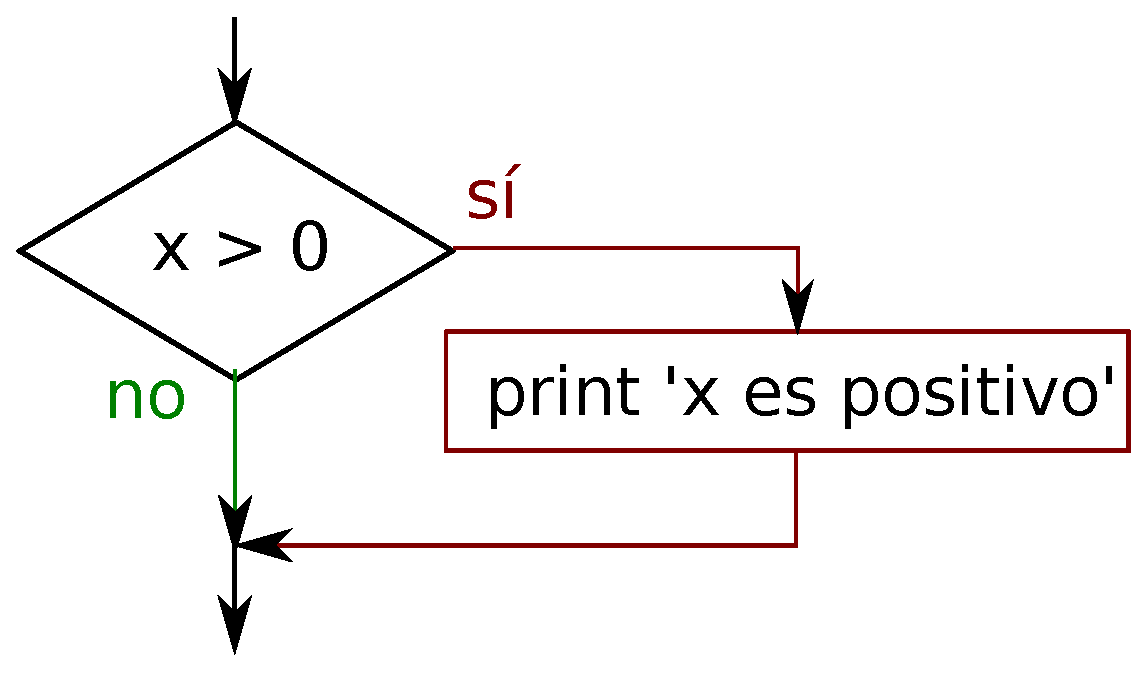
\includegraphics[height=1.75in]{figs2/if.eps}}
\afterfig

Si la condición lógica es verdadera, la sentencia sangrada
es ejecutada. Si la condición es falsa,
la sentencia sangrada es omitida.

\index{condición}
\index{compuesta, sentencia}
\index{sentencia!compuesta}

La sentencia {\tt if} tiene la misma estructura que la definición de funciones
o los bucles {\tt for}\footnote{Estudiaremos las funciones en el capítulo 4
y los bucles en el capítulo 5.}. La sentencia consiste en una línea de encabezado
que termina con el carácter dos-puntos (:)
seguido por un bloque con sangrado. Las sentencias de este tipo
reciben el nombre de {\bf sentencias compuestas}, porque se extienden
a lo largo de varias líneas.

No hay límite en el número de sentencias que pueden aparecer en el
cuerpo, pero debe haber al menos una.
Ocasionalmente, puede resultar útil tener un cuerpo sin sentencias
(normalmente como emplazamiento reservado para código que no se ha escrito aún). En ese
caso, se puede usar la sentencia {\tt pass}, que no hace nada.

\index{pass, sentencia}
\index{sentencia!pass}

\beforeverb
\begin{verbatim}
if x < 0 :
    pass          # ¡necesito controlar los valores negativos!
\end{verbatim}
\afterverb
%
Si introduces una sentencia {\tt if} en el intérprete de Python, el prompt cambiará
su aspecto habitual por puntos suspensivos, para indicar que estás en medio de un bloque de sentencias, como
se muestra a continuación:

\beforeverb
\begin{verbatim}
>>> x = 3
>>> if x < 10:
...    print 'Pequeño'
... 
Pequeño
>>>
\end{verbatim}
\afterverb
%

\section{Ejecución alternativa}
\label{alternative execution}

\index{ejecución alternativa}
\index{else, palabra clave}
\index{palabra clave!else}

La segunda forma de la sentencia {\tt if} es la {\bf ejecución alternativa},
en la cual existen dos posibilidades y la condición determina
cual de ellas será ejecutada. La sintaxis es similar a ésta:

\beforeverb
\begin{verbatim}
if x%2 == 0 :
    print 'x es par'
else :
    print 'x es impar'
\end{verbatim}
\afterverb
%
Si al dividir {\tt x} por 2 obtenemos como resto 0, entonces sabemos
que {\tt x} es par, y el programa muestra un mensaje a tal
efecto. Si esa condición es falsa, se ejecuta el segundo
conjunto de sentencias.

\beforefig
\centerline{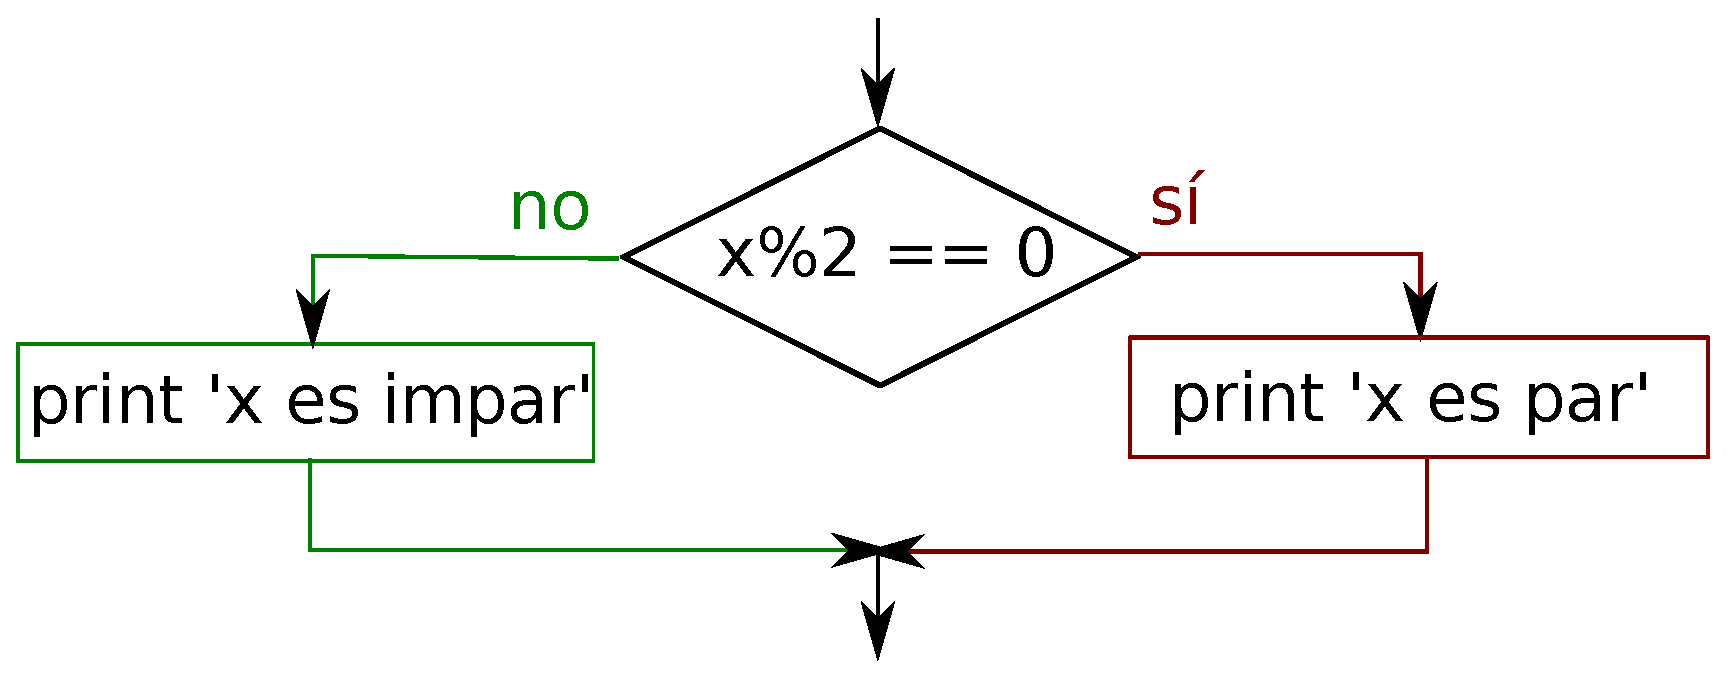
\includegraphics[height=1.75in]{figs2/if-else.eps}}
\afterfig

Dado que la condición debe ser obligatoriamente verdadera o falsa, solamente una de
las alternativas será ejecutada. Las alternativas reciben el nombre de
{\bf ramas}, dado que se trata de ramificaciones en el flujo de la ejecución.

\index{branch}

\section{Condicionales encadenados}
\index{encadenado, condicional}
\index{condicional!encadenado}

Algunas veces hay más de dos posibilidades, de modo que necesitamos más
de dos ramas. Una forma de expresar un cálculo como ése es usar un
{\bf condicional encadenado}:

\beforeverb
\begin{verbatim}
if x < y:
    print 'x es menor que y'
elif x > y:
    print 'x es mayor que y'
else:
    print 'x e y son iguales'
\end{verbatim}
\afterverb
%
{\tt elif} es una abreviatura para ``else if''.  En este caso también
será ejecutada únicamente una de las ramas.

\beforefig
\centerline{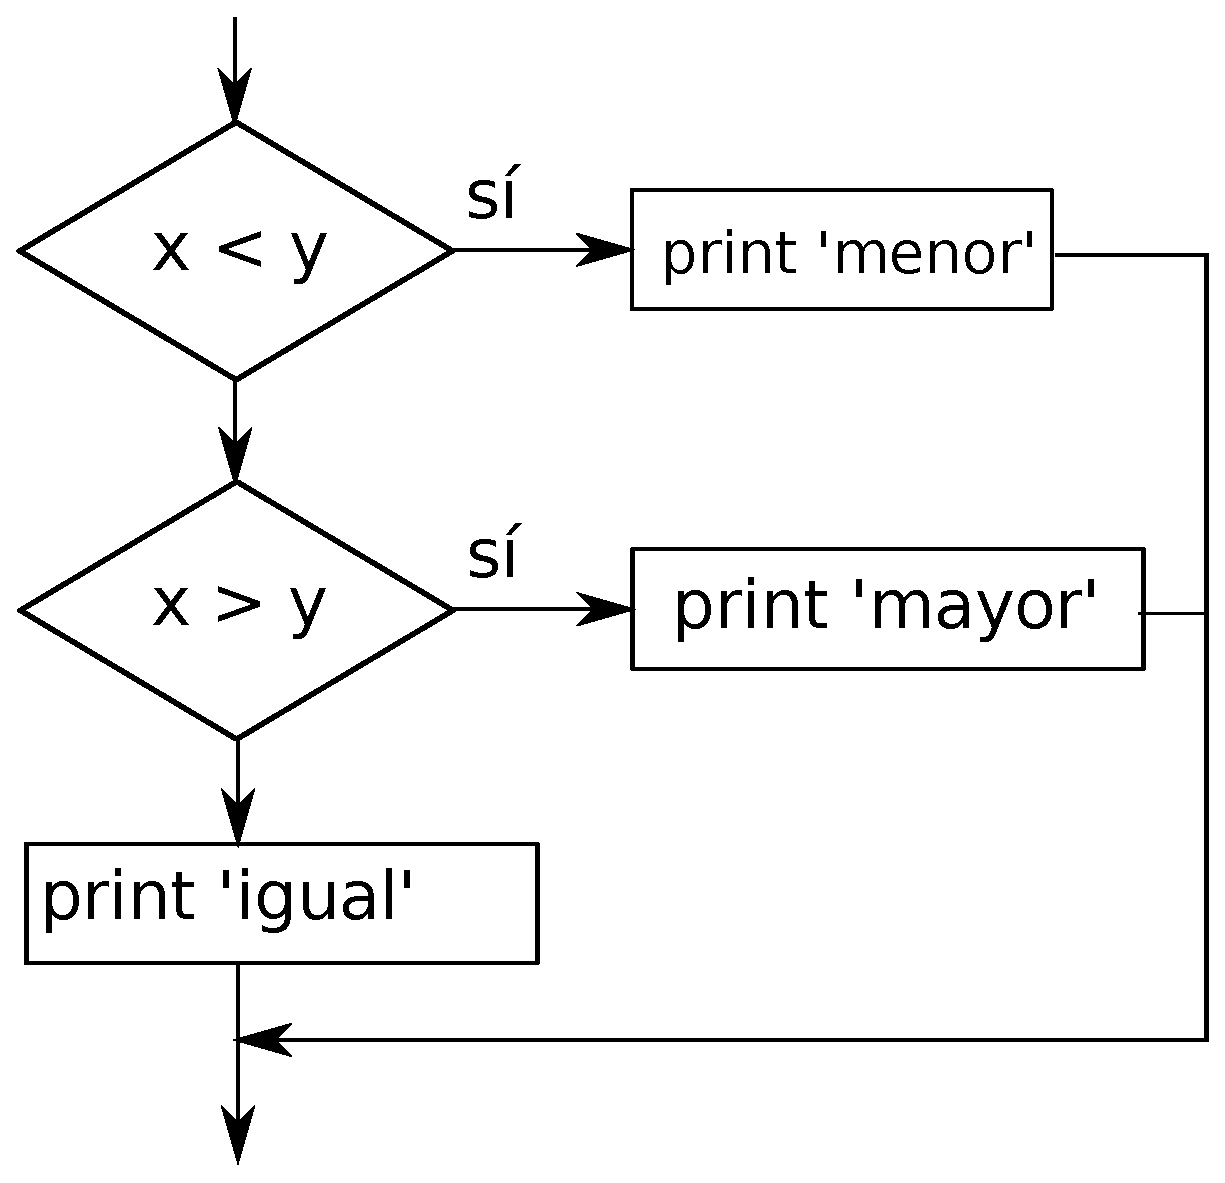
\includegraphics[height=3.00in]{figs2/elif.eps}}
\afterfig

No hay un límite para el número de sentencias
{\tt elif}. Si hay una clausula {\tt else}, debe ir
al final, pero tampoco es obligatorio que ésta exista.

\index{elif, palabra clave}
\index{palabra clave!elif}


\beforeverb
\begin{verbatim}
if choice == 'a':
    print 'Respuesta incorrecta'
elif choice == 'b':
    print 'Respuesta correcta'
elif choice == 'c':
    print 'Casi, pero no es correcto'
\end{verbatim}
\afterverb
%
Cada condición es comprobada en orden. Si la primera es falsa,
se comprueba la siguiente y así con las demás. Si una de ellas es
verdadera, se ejecuta la rama correspondiente, y la sentencia
termina. Incluso si hay más de una condición que sea verdadera, sólo se
ejecuta la primera que se encuentra.

\section{Condicionales anidados}
\index{anidado, condicional}
\index{condicional!anidado}

Un condicional puede también estar anidado dentro de otro. Podríamos
haber escrito el ejemplo anterior de las tres ramas de este modo:

\beforeverb
\begin{verbatim}
if x == y:
    print 'x e y son iguales'
else:
    if x < y:
        print 'x es menor que y'
    else:
        print 'x es mayor que y'
\end{verbatim}
\afterverb
%
El condicional exterior contiene dos ramas. La
primera rama ejecuta una sentencia simple. La segunda
contiene otra sentencia {\tt if}, que tiene a su vez sus propias
dos ramas. Esas dos ramas son ambas sentencias simples,
pero podrían haber sido sentencias condicionales también.

\beforefig
\centerline{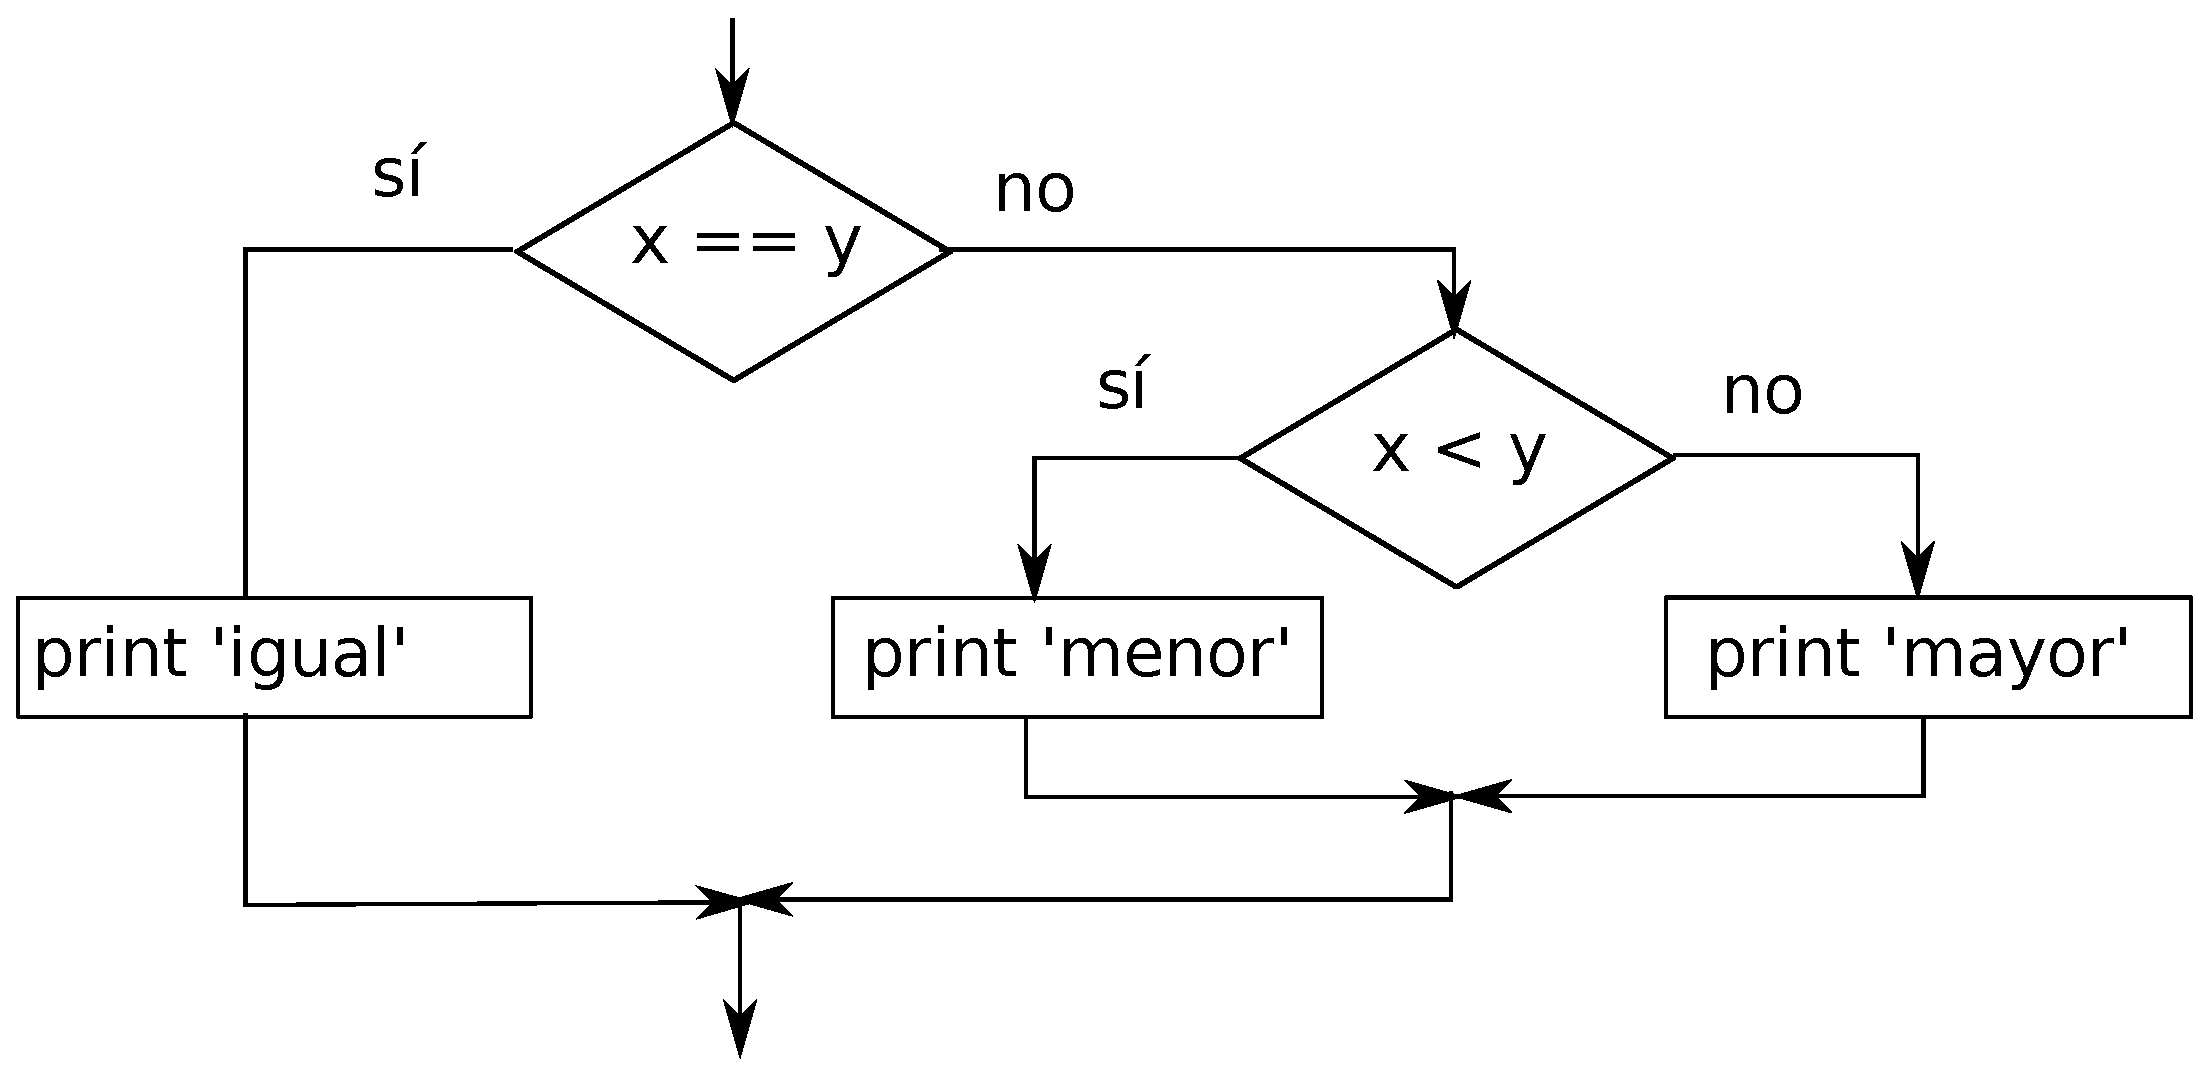
\includegraphics[height=2.50in]{figs2/nested.eps}}
\afterfig

A pesar de que el sangrado de las sentencias hace que la estructura
esté clara, los {\bf condicionales anidados} pueden volverse difíciles
de leer rápidamente. En general, es buena idea evitarlos si se puede.

Los operadores lógicos a menudo proporcionan un modo de simplificar las
sentencias condicionales anidadas. Por ejemplo, el código siguiente
puede ser reescrito usando un único condicional:

\beforeverb
\begin{verbatim}
if 0 < x:
    if x < 10:
        print 'x es un número positivo con un sólo dígito.'
\end{verbatim}
\afterverb
%
La sentencia {\tt print} se ejecuta solamente si se cumplen las dos condiciones
anteriores, así que en realidad podemos conseguir el mismo efecto con el operador {\tt and}:

\beforeverb
\begin{verbatim}
if 0 < x and x < 10:
    print 'x es un número positivo con un sólo dígito.'
\end{verbatim}
\afterverb


\section{Captura de excepciones usando try y except}
\label{catch1}

Anteriormente vimos un fragmento de código donde usábamos las funciones \verb"raw_input" e
{\tt int} para leer y analizar un número entero introducido por
el usuario. También vimos lo poco seguro que podía llegar a ser hacer algo así:

\beforeverb
\begin{verbatim}
>>> velocidad = raw_input(prompt)
¿Cual.... es la velocidad de vuelo de una golondrina sin carga?
¿Te refieres a una golondrina africana o a una europea?
>>> int(velocidad)
ValueError: invalid literal for int()
>>>
\end{verbatim}
\afterverb
%
Cuando estamos trabajando con el intérprete de Python, tras el error simplemente
nos aparece de nuevo el prompt, así que pensamos ``¡epa, me he equivocado!'', y continuamos
con la siguiente sentencia.

Sin embargo, si se escribe ese código en un
script de Python y se produce el error, el script se detendrá
inmediatamente, y mostrará un ``traceback''.
No ejecutará la siguiente sentencia.

\index{traceback}

He aquí un programa de ejemplo para convertir una temperatura
desde grados Fahrenheit a grados Celsius:

\index{fahrenheit}
\index{celsius}
\index{conversión de temperatura}

\beforeverb
\begin{verbatim}
ent = raw_input('Introduce la Temperatura Fahrenheit:')
fahr = float(ent)
cel = (fahr - 32.0) * 5.0 / 9.0
print cel
\end{verbatim}
\afterverb
%
Si ejecutamos este código y le damos una entrada no válida, simplemente
fallará con un mensaje de error bastante antipático:

\beforeverb
\begin{verbatim}
python fahren.py 
Introduce la Temperatura Fahrenheit:72
22.2222222222

python fahren.py 
Introduce la Temperatura Fahrenheit:fred
Traceback (most recent call last):
  File "fahren.py", line 2, in <module>
    fahr = float(ent)
ValueError: invalid literal for float(): fred
\end{verbatim}
\afterverb
%
Existen estructuras de ejecución condicional dentro de
Python para manejar este tipo de errores esperados e
inesperados, llamadas ``try / except''. La idea de {\tt try}
y {\tt except} es que si se sabe que cierta secuencia
de instrucciones puede generar un problema, sea posible
añadir ciertas sentencias para que sean ejecutadas en caso de error.
Estas sentencias extras (el bloque except) serán ignoradas
si no se produce ningún error.

Puedes pensar en la característica {\tt try} y {\tt except}
de Python como una ``póliza de seguros'' en una secuencia
de sentencias.

Se puede reescribir nuestro conversor de temperaturas de esta forma:

\beforeverb
\begin{verbatim}
ent = raw_input('Introduce la Temperatura Fahrenheit:')
try:
    fahr = float(ent)
    cel = (fahr - 32.0) * 5.0 / 9.0
    print cel
except:
    print 'Por favor, introduce un número'
\end{verbatim}
\afterverb
%

Python comienza ejecutando la
secuencia de sentencias del bloque
{\tt try}. Si todo va bien,
saltará el bloque {\tt except} y terminará.
Si ocurre una excepción dentro del bloque {\tt try},
Python saltará fuera de ese bloque y
ejecutará la secuencia de sentencias en el bloque {\tt except}.

\beforeverb
\begin{verbatim}
python fahren2.py 
Introduce la Temperatura Fahrenheit:72
22.2222222222

python fahren2.py 
Introduce la Temperatura Fahrenheit:fred
Por favor, introduce un número
\end{verbatim}
\afterverb
%

Manejar una excepción con una sentencia {\tt try} recibe el nombre de
{\bf capturar} una excepción. En este ejemplo, la clausula {\tt except}
muestra un mensaje de error. En general,
capturar una excepción te da la oportunidad de corregir el problema,
volverlo a intentar, o al menos de terminar el programa con elegancia.

\section{Evaluación en cortocircuito de expresiones lógicas}
\index{cortocircuito}

Cuando Python está procesando una expresión lógica, como
{\tt x >= 2 and (x/y) > 2}, evalúa la expresión de
izquierda a derecha. Debido a la definición de {\tt and},
si {\tt x} es menor de 2, la expresión {\tt x >= 2} resulta ser
{\tt falsa}, de modo que la expresión completa ya va a resultar {\tt falsa}, independientemente
de si {\tt (x/y) > 2} se evalúa como {\tt verdadero} o {\tt falso}.

Cuando Python detecta que no se gana nada evaluando
el resto de una expresión lógica, detiene su evaluación y no
realiza el cálculo del resto de la expresión.
Cuando la evaluación de una expresión lógica se detiene debido a que
ya se conoce el valor final, esto es conocido como {\bf cortocircuitar}
la evaluación.

\index{guardián, patrón}
\index{patrón!guardián}
A pesar de que esto pueda parecer hilar demasiado fino, el funcionamiento
en cortocircuito nos descubre una ingeniosa técnica conocida como {\bf patrón guardián}.
Considera la siguiente secuencia de código en el intérprete de Python:

\beforeverb
\begin{verbatim}
>>> x = 6 
>>> y = 2
>>> x >= 2 and (x/y) > 2
True
>>> x = 1 
>>> y = 0
>>> x >= 2 and (x/y) > 2
False
>>> x = 6
>>> y = 0
>>> x >= 2 and (x/y) > 2
Traceback (most recent call last):
  File "<stdin>", line 1, in <module>
ZeroDivisionError: integer division or modulo by zero
>>> 
\end{verbatim}
\afterverb
%
El tercer cálculo ha fallado porque Python intentó evaluar {\tt (x/y)}
e {\tt y} era cero, lo cual provoca un runtime error (error en tiempo de ejecución). Pero el segundo
ejemplo \emph{no} falló, porque la primera parte de la expresión {\tt x >= 2}
fue evaluada como {\tt falsa}, así que {\tt (x/y)} no llegó a ejecutarse
debido a la regla del {\bf cortocircuito}, y no se produjo ningún error.

Es posible construir las expresiones lógicas colocando estratégicamente una
evaluación como {\bf guardián} justo antes de la evaluación que podría causar un error,
como se muestra a continuación:

\beforeverb
\begin{verbatim}
>>> x = 1
>>> y = 0
>>> x >= 2 and y != 0 and (x/y) > 2
False
>>> x = 6 
>>> y = 0
>>> x >= 2 and y != 0 and (x/y) > 2
False
>>> x >= 2 and (x/y) > 2 and y != 0
Traceback (most recent call last):
  File "<stdin>", line 1, in <module>
ZeroDivisionError: integer division or modulo by zero
>>>
\end{verbatim}
\afterverb
%
En la primera expresión lógica, {\tt x >= 2} es {\tt falsa}, así que la evaluación
se detiene en el {\tt and}. En la segunda expresión lógica, {\tt x >= 2} es {\tt verdadera},
pero {\tt y != 0} es {\tt falsa}, de modo que nunca se alcanza {\tt (x/y)}.

En la tercera expresión lógica, el {\tt y != 0} va \emph{después} del
cálculo de {\tt (x/y) }, de modo que la expresión falla con un error.

En la segunda expresión, se dice que {\tt y != 0} actúa como {\bf guardián}
para asegurar que sólo se ejecute {\tt (x/y)} en el caso de que {\tt y} no sea cero.


\section{Depuración}
\label{whitespace}
\index{depuración}
\index{traceback}

Los ``traceback'' que Python muestra cuando se produce un error contienen
un montón de información, pero pueden resultar abrumadores. Las partes
más útiles normalmente son:

\begin{itemize}

\item Qué tipo de error se ha producido, y

\item Dónde ha ocurrido.

\end{itemize}

Los errores de sintaxis (syntax errors), normalmente son fáciles de encontrar, pero
a veces tienen trampa. Los errores debido a espacios en blanco pueden ser complicados de
localizar, ya que los espacios y las tabulaciones son invisibles, y solemos ignorarlos.

\index{espacio en blanco}

\beforeverb
\begin{verbatim}
>>> x = 5
>>>  y = 6
  File "<stdin>", line 1
    y = 6
    ^
SyntaxError: invalid syntax
\end{verbatim}
\afterverb
%
En este ejemplo, el problema es que la segunda línea está sangrada por
un espacio. Pero el mensaje de error apunta a {\tt y}, lo cual
resulta engañoso. En general, los mensajes de error indican dónde se ha
descubierto el problema, pero el error real podría estar en el código
previo, a veces en alguna línea anterior.

\index{error!runtime}
\index{runtime error}

Ocurre lo mismo con los errores en tiempo de ejecución (runtime errors). Supón que estás tratando
de calcular una relación señal-ruido en decibelios. La fórmula
es $SNR_{db} = 10 \log_{10} (P_{señal} / P_{ruido})$. En Python,
podrías escribir algo como esto:

\beforeverb
\begin{verbatim}
import math
int_senal = 9
int_ruido = 10
relacion = int_senal / int_ruido
decibelios = 10 * math.log10(relacion)
print decibelios
\end{verbatim}
\afterverb
%
Pero cuando lo haces funcionar, obtienes un mensaje de error\footnote{En Python 3.0,
ya no se produce el mensaje de error; el operador de división realiza
división en punto flotante incluso con operandos enteros.}:

\index{exception!OverflowError}
\index{OverflowError}

\beforeverb
\begin{verbatim}
Traceback (most recent call last):
  File "snr.py", line 5, in ?
    decibelios = 10 * math.log10(relacion)
OverflowError: math range error
\end{verbatim}
\afterverb
%
El mensaje de error apunta a la línea 5, pero no hay nada
incorrecto en ese línea. Para encontrar el error real, puede resultar
útil mostrar en pantalla el valor de {\tt relacion}, que resulta ser
0. El problema está en la línea 4, ya que al dividir dos enteros
se realiza una división entera. La solución es representar la intensidad
de la señal y la intensidad del ruido con valores en punto flotante.

\index{entera, division}
\index{división!entera}

En general, los mensajes de error te dicen dónde se ha descubierto el problema,
pero a menudo no es ahí exactamente donde se ha producido.


\section{Glosario}

\begin{description}

\item[condición:] La expresión booleana en una sentencia condicional
que determina qué rama será ejecutada.
\index{condición}

\item[condicional anidado:]  Una sentencia condicional que aparece
en una de las ramas de otra sentencia condicional.
\index{anidado, condicional}
\index{condicional!anidado}

\item[condicional encadenado:]  Una sentencia condicional con una serie
de ramas alternativas.
\index{encadenado, condicional}
\index{condicional!encadenado}
	
\item[cortocircuito:]  Cuando Python va evaluando una expresión lógica
por tramos y detiene el proceso de evaluación debido a que ya
conoce el valor final que va a tener el resultado
sin necesidad de evaluar el resto de la expresión.
\index{cortocircuito}

\item[cuerpo:] La secuencia de sentencias en el interior de una sentencia compuesta.
\index{cuerpo}

\item[expresión booleana:]  Un expresión cuyo valor puede ser o bien 
{\tt Verdadero} o bien {\tt Falso}.
\index{booleana, expresión}
\index{expresión!booleana}

\item[operadores de comparación:] Uno de los operadores que se utiliza para comparar
dos operandos: {\tt ==}, {\tt !=}, {\tt \verb">"}, {\tt \verb"<"}, {\tt \verb">="}, y {\tt \verb"<="}.

\item[operador lógico:] Uno de los operadores que se combinan en las expresiones
booleanas: {\tt and}, {\tt or}, y {\tt not}.

\item[patrón guardián:] Cuando construimos una expresión lógica
con comparaciones adicionales
para aprovecharnos del funcionamiento en cortocircuito.
\index{guardián, patrón}
\index{patrón!guardián}

\item[rama:] Una de las secuencias alternativas de sentencias en una
sentencia condicional.
\index{rama}

\item[sentencia compuesta:]  Una sentencia que consiste en un encabezado
y un cuerpo. El encabezado termina con dos-puntos (:). El cuerpo está sangrado
con relación al encabezado.
\index{compuesta, sentencia}
\index{sentencia!compuesta}

\item[sentencia condicional:]  Una sentencia que controla el flujo de
ejecución, dependiendo de cierta condición.
\index{condicional, sentencia}
\index{sentencia!condicional}

\item[traceback:]  Una lista de las funciones que se están ejecutando,
que se muestra en pantalla cuando se produce una excepción.
\index{traceback}

\end{description}

\section{Ejercicios}

\begin{ex}
Reescribe el programa del cálculo del salario para darle al empleado 1.5
veces la tarifa horaria para todas
las horas trabajadas que excedan de 40.

\begin{verbatim}
Introduce las Horas: 45
Introduce la Tarifa por hora: 10
Salario: 475.0
\end{verbatim}
\end{ex}

\begin{ex}
Reescribe el programa del salario usando {\tt try} y {\tt except},
de modo que el programa sea capaz de gestionar entradas no numéricas con elegancia,
mostrando un mensaje y saliendo del programa.
A continuación se muestran dos ejecuciones del programa:

\begin{verbatim}
Introduce las Horas: 20
Introduce la Tarifa por hora: nueve
Error, por favor introduce un número

Introduce las Horas: cuarenta
Error, por favor introduce un número
\end{verbatim}
\end{ex}

\begin{ex}
Escribe un programa que solicite una puntuación entre 0.0 y 1.0.
Si la puntuación está fuera de ese rango, muestra un mensaje de error.
Si la puntuación está entre 0.0 y 1.0, muestra la calificación usando la tabla
siguiente:

\begin{verbatim}
Puntuación Calificación
>= 0.9     Sobresaliente
>= 0.8     Notable
>= 0.7     Bien
>= 0.6     Suficiente
< 0.6      Insuficiente

Introduce puntuación: 0.95
Sobresaliente

Introduce puntuación: perfecto
Puntuación incorrecta

Introduce puntuación: 10.0
Puntuación incorrecta

Introduce puntuación: 0.75
Bien

Introduce puntuación: 0.5
Insuficiente
\end{verbatim}

Ejecuta el programa repetidamente, como se muestra arriba, para probar
con varios valores de entrada diferentes.
\end{ex}
% LaTeX source for ``Python for Informatics: Exploring Information''
% Copyright (c)  2010-  Charles R. Severance, All Rights Reserved

\chapter{Funciones}
\label{funcchap}

\section{Llamadas a funciones}
\label{functionchap}
\index{function call}

En el contexto de la programación, una {\bf función} es una secuencia de
sentencias que realizan un cálculo y que reciben un nombre. Cuando se define una función,
es posible especificar el nombre y la secuencia de sentencias. Más adelante, se puede
``llamar'' a la función por ese nombre.
Ya hemos visto un ejemplo de una {\bf llamada a una función}:

\beforeverb
\begin{verbatim}
>>> type(32)
<type 'int'>
\end{verbatim}
\afterverb
%
El nombre de la función es {\tt type}. La expresión entre paréntesis recibe
el nombre de {\bf argumento} de la función. El argumento es
un valor o variable que se pasa a la función como parámetro de entrada.
El resultado de la función {\tt type} es el tipo del argumento.

\index{parentheses!argument in}

Es habitual decir que una función ``toma'' un argumento y ``retorna'' (o devuelve)
un resultado. El resultado se llama {\bf valor de retorno}.

\index{argument}
\index{return value}

\section{Funciones incorporadas}

Python proporciona un número importante de funciones incorporadas, que
pueden ser usadas sin necesidad de tener que definirlas previamente.
Los creadores de Python han escrito un conjunto de funciones
para resolver problemas comunes y las han incluido en Python para que las podamos utilizar.

Las funciones {\tt max} y {\tt min} nos darán respectivamente
el valor mayor y menor de una lista:

\beforeverb
\begin{verbatim}
>>> max('¡Hola, mundo!')
'u'
>>> min('¡Hola, mundo!')
' '
>>>
\end{verbatim}
\afterverb
%
La función {\tt max} nos dice cuál es el ``carácter más grande'' de la
cadena (que resulta ser la letra ``u''), mientras que la función
{\tt min} nos muestra el carácter más pequeño (que en ese caso es
un espacio).

Otra función incorporada muy común es {\tt len},
que nos dice cuántos elementos hay en su argumento. Si el argumento
de {\tt len} es una cadena, nos devuelve el número de caracteres
que hay en la cadena.

\beforeverb
\begin{verbatim}
>>> len('Hola, mundo')
11
>>>
\end{verbatim}
\afterverb
%
Estas funciones no se limitan a buscar en cadenas. Pueden operar con
cualquier conjunto de valores, como veremos en los siguientes capítulos.

Se deben tratar los nombres de las funciones incorporadas como si fueran palabras reservadas
(es decir, evita usar ``max'' como nombre para una variable).

\section{Funciones de conversión de tipos}
\index{conversion!type}
\index{type conversion}

% de Elkner:
% comentario acerca de si estas cosas son realmente funciones
% ¿usar max como ejemplo de una función incorporada?

% mi respuesta:
% están en la lista de ``funciones incorporadas'', de modo que estoy dispuesto
% a llamarlas funciones.

Python también proporciona funciones incorporadas que convierten valores
de un tipo a otro. La función {\tt int} toma cualquier valor y
lo convierte en un entero si puede, o se queja si no puede:

\index{int function}
\index{function!int}

\beforeverb
\begin{verbatim}
>>> int('32')
32
>>> int('Hola')
ValueError: invalid literal for int(): Hola
\end{verbatim}
\afterverb
%
{\tt int} puede convertir valores en punto flotante a enteros, pero no
los redondea; simplemente corta y descarta la parte decimal:

\beforeverb
\begin{verbatim}
>>> int(3.99999)
3
>>> int(-2.3)
-2
\end{verbatim}
\afterverb
%
{\tt float} convierte enteros y cadenas en números
de punto flotante:

\index{float function}
\index{function!float}

\beforeverb
\begin{verbatim}
>>> float(32)
32.0
>>> float('3.14159')
3.14159
\end{verbatim}
\afterverb
%
Finalmente, {\tt str} convierte su argumento en una cadena:

\index{str function}
\index{function!str}

\beforeverb
\begin{verbatim}
>>> str(32)
'32'
>>> str(3.14159)
'3.14159'
\end{verbatim}
\afterverb
%

\section{Números aleatorios}

\index{random number}
\index{number, random}
\index{deterministic}
\index{pseudorandom}

A partir de las mismas entradas, la mayoría de los ordenadores generarán
las mismas salidas cada vez, que es lo que llamamos comportamiento {\bf determinista}.
El determinismo normalmente es algo bueno, ya que esperamos que el mismo
cálculo nos proporcione siempre el mismo resultado. Para ciertas aplicaciones, sin embargo,
querremos que el ordenador sea impredecible. Los juegos son el ejemplo
obvio, pero hay más.

Conseguir que un programa sea realmente no-determinista no resulta tan fácil,
pero hay modos de hacer que al menos lo parezca. Una de ellos
es usar {\bf algoritmos} que generen números {\bf pseudoaleatorios}.
Los números pseudoaleatorios no son verdaderamente aleatorios, ya que son
generados por un cálculo determinista, pero si sólo nos fijamos en los números
resulta casi imposible distinguirlos de los aleatorios de verdad.

\index{random module}
\index{module!random}

El módulo {\tt random} proporciona funciones que generan
números pseudoaleatorios (a los que simplemente llamaremos ``aleatorios''
de ahora en adelante).

\index{random function}
\index{function!random}

La función {\tt random} devuelve un número flotante aleatorio
entre 0.0 y 1.0 (incluyendo 0.0, pero no 1.0). Cada vez que se
llama a {\tt random}, se obtiene el número siguiente de una larga serie. Para ver
un ejemplo, ejecuta este bucle:

\beforeverb
\begin{verbatim}
import random

for i in range(10):
    x = random.random()
    print x
\end{verbatim}
\afterverb
%
Este programa produce la siguiente lista de 10 números aleatorios
entre 0.0 y hasta (pero no incluyendo) 1.0.

\beforeverb
\begin{verbatim}
0.301927091705
0.513787075867
0.319470430881
0.285145917252
0.839069045123
0.322027080731
0.550722110248
0.366591677812
0.396981483964
0.838116437404
\end{verbatim}
\afterverb
%
\begin{ex}
Ejecuta el programa en tu sistema y observa qué números obtienes.
\end{ex}

La función {\tt random} es solamente una de las muchas
que trabajan con números aleatorios.
La función {\tt randint} toma los parámetros {\tt inferior} y
{\\ superior}, y devuelve un entero entre {\tt inferior} y 
{\tt superior} (incluyendo ambos extremos).

\index{randint function}
\index{function!randint}

\beforeverb
\begin{verbatim}
>>> random.randint(5, 10)
5
>>> random.randint(5, 10)
9
\end{verbatim}
\afterverb
%
Para elegir un elemento de una secuencia aleatoriamente, se puede usar
{\tt choice}:

\index{choice function}
\index{function!choice}

\beforeverb
\begin{verbatim}
>>> t = [1, 2, 3]
>>> random.choice(t)
2
>>> random.choice(t)
3
\end{verbatim}
\afterverb
%
El módulo {\tt random} también proporciona funciones para generar
valores aleatorios de distribuciones continuas, incluyendo
Gausiana, exponencial, gamma, y unas cuantas más.

\section{Funciones matemáticas}
\index{math function}
\index{function, math}
\index{module}
\index{module object}

Python tienen un módulo {\tt matemático (math)}, que proporciona la mayoría
de las funciones matemáticas habituales.
Antes de que se pueda utilizar el módulo, hay que importarlo:

\beforeverb
\begin{verbatim}
>>> import math
\end{verbatim}
\afterverb
%
Esta sentencia crea un {\bf objeto módulo} llamado math. Si
se imprime el objeto módulo, se obtiene cierta información sobre él:

\beforeverb
\begin{verbatim}
>>> print math
<module 'math' from '/usr/lib/python2.5/lib-dynload/math.so'>
\end{verbatim}
\afterverb
%
El objeto módulo contiene la función y variables definidas en el módulo.
Para acceder a una de esas funciones, es necesario especificar el nombre
del módulo y el nombre de la función, separados por un punto (también
conocido como período). Este formato recibe el nombre de {\bf notación punto}.

\index{dot notation}

\beforeverb
\begin{verbatim}
>>> relacion = int_senal / int_ruido
>>> decibelios = 10 * math.log10(relacion)

>>> radianes = 0.7
>>> altura = math.sin(radianes)
\end{verbatim}
\afterverb
%
El primer ejemplo calcula el logaritmo base 10 de la
relación señal-ruido. El módulo math también proporciona una
función llamada {\tt log} que calcula logaritmos en base {\tt e}.

\index{log function}
\index{function!log}
\index{sine function}
\index{radian}
\index{trigonometric function}
\index{function, trigonometric}

El segundo ejemplo calcula el seno de la variable {\tt radianes}. El nombre de la
variable es una pista de que {\tt sin} y las otras funciones
trigonométricas ({\tt cos}, {\tt tan}, etc.) toman argumentos en radianes.
Para convertir de grados a radianes, hay que dividir por 360 y multiplicar por
$2\pi$:

\beforeverb
\begin{verbatim}
>>> grados = 45
>>> radianes = grados / 360.0 * 2 * math.pi
>>> math.sin(radianes)
0.707106781187
\end{verbatim}
\afterverb
%
La expresión {\tt math.pi} toma la variable {\tt pi} del módulo math.
El valor de esa variable es una aproximación de
$\pi$, con una precisión de unos 15 dígitos.

\index{pi}

Si sabes de
trigonometría, puedes comprobar el resultado anterior, comparándolo con
la raíz cuadrada de dos dividida por dos:

\index{sqrt function}
\index{function!sqrt}

\beforeverb
\begin{verbatim}
>>> math.sqrt(2) / 2.0
0.707106781187
\end{verbatim}
\afterverb
%


\section{Añadiendo funciones nuevas}

Hasta ahora, sólo hemos estado usando las funciones que vienen incorporadas en Python,
pero es posible añadir también funciones nuevas.
Una {\bf definición de función} especifica el nombre de una función nueva y
la secuencia de sentencias que se ejecutan cuando esa función es llamada.
Una vez definida una función, se puede reutilizar una y otra vez
a lo largo de todo el programa.

\index{function}
\index{function definition}
\index{definition!function}

He aquí un ejemplo:

\beforeverb
\begin{verbatim}
def print_lyrics():
    print "Soy un leñador, qué alegría."
    print 'Duermo toda la noche y trabajo todo el día.'
\end{verbatim}
\afterverb
%
{\tt def} es una palabra clave que indica que se trata de una definición
de función. El nombre de la función es \verb"print_lyrics". Las
reglas para los nombres de las funciones son los mismos que para las variables:
se pueden usar letras, números y algunos signos de puntuación, pero el primer carácter
no puede ser un número. No se pueden usar una palabra clave como nombre de una función,
y se debería evitar tener una variable y una función con el mismo
nombre.

\index{def keyword}
\index{keyword!def}
\index{argument}

Los paréntesis vacíos después del nombre indican que esta función
no toma ningún argumento. Más tarde construiremos funciones que
toman argumentos de entrada.

\index{parentheses!empty}
\index{header}
\index{body}
\index{indentation}
\index{colon}

La primera línea de la definición de la función es llamada la {\bf cabecera};
el resto se llama el {\bf cuerpo}. La cabecera debe terminar con dos-puntos (:),
y el cuerpo debe ir sangrado. Por convención, el sangrado es
siempre de cuatro espacios. El cuerpo puede contener
cualquier número de sentencias.

Las cadenas en la sentencia print están encerradas entre
comillas. Da igual utilizar comillas simples que dobles;
la mayoría de la gente prefiere comillas simples, excepto en aquellos casos en los que
una comilla simple (que también se usa como apostrofe) aparece en medio de la cadena.

\index{ellipses}

Si escribes una definición de función en modo interactivo, el intérprete
mostrará puntos suspensivos (\emph{...}) para informarte de que la definición
no está completa:

\beforeverb
\begin{verbatim}
>>> def print_lyrics():
...     print "Soy un leñador, qué alegría."
...     print 'Duermo toda la noche y trabajo todo el día.'
...
\end{verbatim}
\afterverb
%
Para finalizar la función, debes introducir una línea vacía (esto no
es necesario en un script).

Al definir una función se crea una variable con el mismo nombre.

\beforeverb
\begin{verbatim}
>>> print print_lyrics
<function print_lyrics at 0xb7e99e9c>
>>> print type(print_lyrics)
<type 'function'>
\end{verbatim}
\afterverb
%
El valor de \verb"print_lyrics" es {\bf function object (objeto función)}, que
tiene como tipo \verb"'function'".

\index{function object}
\index{object!function}

La sintaxis para llamar a la nueva función es la misma que
la de las funciones incorporadas:

\beforeverb
\begin{verbatim}
>>> print_lyrics()
Soy un leñador, qué alegría.
Duermo toda la noche y trabajo todo el día.
\end{verbatim}
\afterverb
%
Una vez que se ha definido una función, puede usarse dentro de otra.
Por ejemplo, para repetir el estribillo anterior, podríamos escribir
una función llamada \verb"repeat_lyrics":

\beforeverb
\begin{verbatim}
def repeat_lyrics():
    print_lyrics()
    print_lyrics()
\end{verbatim}
\afterverb
%
Y después llamar a \verb"repeat_lyrics":

\beforeverb
\begin{verbatim}
>>> repeat_lyrics()
Soy un leñador, qué alegría.
Duermo toda la noche y trabajo todo el día.
Soy un leñador, qué alegría.
Duermo toda la noche y trabajo todo el día.
\end{verbatim}
\afterverb
%
Pero la canción en realidad no es así.

\section{Definición y usos}
\index{function definition}

Reuniendo los fragmentos de código de las secciones anteriores, el
programa completo sería algo esto:

\beforeverb
\begin{verbatim}
def print_lyrics():
    print "Soy un leñador, que alegría."
    print 'Duermo toda la noche y trabajo todo el día.'

def repeat_lyrics():
    print_lyrics()
    print_lyrics()

repeat_lyrics()
\end{verbatim}
\afterverb
%
Este programa contiene dos definiciones de funciones: \verb"print_lyrics" y
\verb"repeat_lyrics". Las definiciones de funciones son ejecutadas exactamente
igual que cualquier otra sentencia, pero lo que se consigue es crear objetos del tipo función. Las
sentencias dentro de esa función no se ejecutarán hasta que no se llame a la función,
y la definición de la función no genera ninguna salida.

\index{use before def}

Como ya te imaginarás, es necesario crear una función antes de que se
pueda ejecutar. En otras palabras, la definición de la función debe ser
ejecutada antes de que la función se llame por primera vez.

\begin{ex}
Mueve la última línea de este programa
hacia arriba, de modo que la llamada a la función aparezca antes que las
definiciones. Ejecuta
el programa y observa qué mensaje
de error obtienes.
\end{ex}

\begin{ex}
Mueve la llamada de la función de nuevo hacia el final,
y coloca la definición de \verb"print_lyrics" después de la definición
de \verb"repeat_lyrics". ¿Qué ocurre cuando haces funcionar este programa?
\end{ex}


\section{Flujo de ejecución}
\index{flow of execution}

Para asegurarnos de que una función está definida antes de usarla por primera vez,
es necesario saber el orden en que las sentencias son ejecutadas, que es lo
que llamamos el {\bf flujo de ejecución}.

La ejecución siempre comienza en la primera sentencia del programa.
Las sentencias son ejecutadas una por una, en orden de arriba hacia abajo.

Las \emph{definiciones} de funciones no alteran el flujo de la ejecución del
programa, pero recuerda que las sentencias dentro de una función no son
ejecutadas hasta que se llama a esa función.

Una llamada a una función es como un desvío en el flujo de la ejecución. En vez
de pasar a la siguiente sentencia, el flujo salta al cuerpo de
la función, ejecuta todas las sentencias que hay allí, y después vuelve
al punto donde lo dejó.

Esto parece bastante simple, hasta que uno recuerda que una función puede
llamar a otra. Cuando está en medio de una función, el programa puede
tener que ejecutar las sentencias de otra función. Pero cuando
está ejecutando esa nueva función, ¡tal vez haya que ejecutar
otra función más todavía!

Afortunadamente, Python es hábil llevando el seguimiento de dónde se encuentra en cada momento, de modo
que cada vez que completa la ejecución de una función, el programa vuelve al punto donde lo dejó
en la función que había llamado a esa. Cuando esto le lleva hasta el final del programa,
simplemente termina.

¿Cuál es la moraleja de esta sórdida historia? Cuando leas un programa, no
siempre te convendrá hacerlo de arriba a abajo. A veces tiene más
sentido seguir el flujo de la ejecución.

\section{Parámetros y argumentos}
\label{parameters}
\index{parameter}
\index{function parameter}
\index{argument}
\index{function argument}

Algunas de las funciones incorporadas que hemos visto necesitan argumentos. Por
ejemplo, cuando se llama a {\tt math.sin}, se le pasa un número
como argumento. Algunas funciones necesitan más de un argumento:
{\tt math.pow} toma dos, la base y el exponente.

Dentro de las funciones, los argumentos son asignados a
variables llamadas {\bf parámetros}. A continuación mostramos un ejemplo
de una función definida por el usuario que recibe un argumento:

\index{parentheses!parameters in}

\beforeverb
\begin{verbatim}
def print_twice(bruce):
    print bruce
    print bruce
\end{verbatim}
\afterverb
%
Esta función asigna el argumento a un parámetro
llamado {\tt bruce}. Cuando la función es llamada, imprime el valor del
parámetro (sea éste lo que sea) dos veces.

Esta función funciona con cualquier valor que pueda ser mostrado en pantalla.

\beforeverb
\begin{verbatim}
>>> print_twice('Spam')
Spam
Spam
>>> print_twice(17)
17
17
>>> print_twice(math.pi)
3.14159265359
3.14159265359
\end{verbatim}
\afterverb
%
Las mismas reglas de composición que se aplican a las funciones incorporadas, también
se aplican a las funciones definidas por el usuario, de modo que podemos usar cualquier tipo
de expresión como argumento para \verb"print_twice":

\index{composition}

\beforeverb
\begin{verbatim}
>>> print_twice('Spam '*4)
Spam Spam Spam Spam
Spam Spam Spam Spam
>>> print_twice(math.cos(math.pi))
-1.0
-1.0
\end{verbatim}
\afterverb
%
El argumento es evaluado antes de que función sea llamada, así
que en los ejemplos, la expresión \verb"'Spam '*4" y
{\tt math.cos(math.pi)} son evaluadas sólo una vez.

\index{argument}

También se puede usar una variable como argumento:

\beforeverb
\begin{verbatim}
>>> michael = 'Eric, la medio-abeja.'
>>> print_twice(michael)
Eric, la medio-abeja.
Eric, la medio-abeja.
\end{verbatim}
\afterverb
%
El nombre de la variable que pasamos como argumento, ({\tt michael}) no
tiene nada que ver con el nombre del parámetro ({\tt bruce}). No
importa cómo se haya llamado al valor en casa (en la llamada);
dentro de \verb"print_twice", siempre se llamará {\tt bruce}.

\section{Funciones fructíferas y funciones huecas}

\index{fruitful function}
\index{void function}
\index{function, fruitful}
\index{function, void} 

Algunas de las funciones que estamos usando, como las matemáticas, producen
resultados; a falta de un nombre mejor, las llamaremos {\bf funciones fructíferas (fruitful functions)}.
Otras funciones, como \verb"print_twice", realizan una
acción, pero no devuelven un valor. A esas las llamaremos {\bf funciones
huecas (void functions)}.

Cuando llamas a una función fructífera, casi siempre
querrás hacer luego algo con el resultado; por ejemplo, puede
que quieras asignarlo a una variable o usarlo como parte de una expresión:

\beforeverb
\begin{verbatim}
x = math.cos(radians)
golden = (math.sqrt(5) + 1) / 2
\end{verbatim}
\afterverb
%
Cuando llamas a una función en modo interactivo, Python muestra
el resultado:

\beforeverb
\begin{verbatim}
>>> math.sqrt(5)
2.2360679774997898
\end{verbatim}
\afterverb
%
Pero en un script, si llamas a una función fructífera y no
almacenas el resultado de la misma en una variable,
¡el valor de retorno se desvanece en la niebla!

\beforeverb
\begin{verbatim}
math.sqrt(5)
\end{verbatim}
\afterverb
%
Este script calcula la raíz cuadrada de 5, pero dado que no almacena
el resultado en una variable ni lo muestra, no resulta en realidad muy útil.

\index{interactive mode}
\index{script mode}

Las funciones huecas pueden mostrar algo en la pantalla o tener cualquier
otro efecto, pero no devuelven un valor. Si intentas asignar
el resultado a una variable, obtendrás un valor especial llamado
{\tt None (nada)}.

\index{None special value}
\index{special value!None}

\beforeverb
\begin{verbatim}
>>> resultado = print_twice('Bing')
Bing
Bing
>>> print resultado
None
\end{verbatim}
\afterverb
%
El valor {\tt None} no es el mismo que la cadena \verb"'None'".
Es un valor especial que tiene su propio tipo:

\beforeverb
\begin{verbatim}
>>> print type(None)
<type 'NoneType'>
\end{verbatim}
\afterverb
%
Para devolver un resultado desde una función, usamos la sentencia {\\return}
dentro de ella. Por ejemplo, podemos crear una función
muy simple llamada {\tt sumados},
que suma dos números y devuelve el resultado.

\beforeverb
\begin{verbatim}
def sumados(a, b):
    suma = a + b
    return suma

x = sumados(3, 5)
print x
\end{verbatim}
\afterverb
%
Cuando se ejecuta este script, la sentencia {\tt print} mostrará ``8'',
ya que la función {\tt sumados} ha sido llamada con 3 y 5 como argumentos.
Dentro de la función, los parámetros {\tt a} y {\tt b} equivaldrán a 3 y a 5
respectivamente. La función calculó la suma de ambos número y la guardó
en una variable local a la función llamada {\tt suma}.
Después usó la sentencia {\tt return}
para enviar el valor calculado de vuelta al código de llamada
como resultado de la función, que fue asignado
a la variable {\tt x} y mostrado en pantalla.

\section{¿Por qué funciones?}
\index{function, reasons for}

Puede no estar muy claro por qué merece la pena molestarse en dividir
un programa en funciones. Existen varias razones:

\begin{itemize}

\item El crear una función nueva te da oportunidad de dar nombre a un grupo
de sentencias, lo cual hace tu programa más fácil de leer, entender,
y depurar.

\item Las funciones pueden hacer un programa más pequeño, al eliminar código
repetido. Además, si quieres hacer cualquier cambio más tarde, sólo tendrás
que hacerlo en un único lugar.

\item Dividir un programa largo en funciones te permite depurar las
partes de una en una y luego ensamblarlas juntas en una sola pieza.

\item Las funciones bien diseñadas a menudo resultan útiles para otros muchos programas.
Una vez que has escrito y depurado una, puedes reutilizarla.

\end{itemize}

A lo largo del resto del libro, a menudo usaremos una definición de función para
explicar un concepto. Parte de la habilidad de crear y usar funciones consiste en llegar a
tener una función que capture correctamente una idea, como ``encontrar el valor
más pequeño en una lista de valores''. Más adelante te mostraremos el código para
encontrar el valor más pequeño de una lista de valores y te lo presentaremos como
una función llamada {\tt min}, que toma una lista de valores como argumento y
devuelve el valor menor de esa lista.


\section{Depuración}
\label{editor}
\index{debugging}

Si estás usando un editor de texto para escribir tus propios scripts, puede
que tengas problemas con los espacios y tabulaciones. El mejor modo de evitar
esos problemas es usar espacios exclusivamente (no tabulaciones). La mayoría
de los editores de texto que reconocen Python lo hacen así por efecto, aunque
hay algunos que no.

\index{whitespace}

Las tabulaciones y los espacios normalmente son invisibles, lo cual hace
que sea difícil depurar los errores que se pueden producir, así que mejor
busca un editor que gestione el sangrado por ti.

Tampoco te olvides de guardar tu programa antes de hacerlo funcionar. Algunos
entornos de desarrollo lo hacen automáticamente, pero otros no.
En ese caso, el programa que estás viendo en el editor de texto
puede no ser el mismo que estás ejecutando en realidad.

¡La depuración puede llevar mucho tiempo si estás haciendo funcionar el
mismo programa erróneo una y otra vez!

Asegúrate que el código que estás examinando es el mismo que estás ejecutando.
Si no estás seguro, pon algo como \verb"print 'hola'" al principio
del programa y hazlo funcionar de nuevo. Si no ves \verb"print 'hola" en la
pantalla, ¡es que no estás ejecutando el programa correcto!


\section{Glosario}

\begin{description}

\item[algoritmo:] Un proceso general para resolver una categoría de problemas.
\index{algorithm}

\item[argumento:] Un valor proporcionado a una función cuando ésta es llamada.
Ese valor se asigna al parámetro correspondiente en la función.
\index{argument}

\item[cabecera:] La primera línea de una definición de función.
\index{header}

\item[cuerpo:] La secuencia de sentencias dentro de la definición de una función.
\index{body}

\item[composición:] Uso de una expresión o sentencia como parte de otra más larga,
\index{composition}

\item[definición de función:] Una sentencia que crea una función nueva,
especificando su nombre, parámetros, y las sentencias que ejecuta.
\index{function definition}

\item[determinístico:] Perteneciente a un programa que hace lo mismo
cada vez que se ejecuta, a partir de las mismas entradas.
\index{deterministic}

\item[función:] Una secuencia de sentencias con un nombre que realizan alguna
operación útil. Las funciones pueden tomar argumentos o no, y pueden
producir un resultado o no.
\index{function}

\item[función fructífera (fruitful function):] Una función que devuelve un valor.
\index{fruitful function}

\item[función hueca (void function):] Una función que no devuelve ningún valor.
\index{void function}

\item[flujo de ejecución:] El orden en el cual las sentencias son ejecutadas durante
el funcionamiento de un programa.
\index{flow of execution}

\item[llamada a función:] Una sentencia que ejecuta una función. Consiste en
el nombre de la función seguido por una lista de argumentos.
\index{function call}

\item[notación punto:] La sintaxis de llamada a una función en
otro módulo, especificando el nombre del módulo seguido por un punto y el
nombre de la función.
\index{dot notation}

\item[objeto función:]  Un valor creado por una definición de función.
El nombre de la función es una variable que se refiere al objeto
función.
\index{function definition}

\item[objeto módulo:] Un valor creado por una sentencia {\tt import},
que proporciona acceso a los datos y código definidos en un módulo.
\index{module}

\item[parámetro:] Un nombre usado dentro de una función para referirse al valor
pasado como argumento.
\index{parameter}

\item[pseudoaleatorio:] Perteneciente a una secuencia de números que parecen
ser aleatorios, pero son generados por un programa determinista.
\index{pseudorandom}

\item[sentencia import:] Una sentencia que lee un archivo módulo y crea
un objeto módulo.
\index{import statement}
\index{statement!import}

\item[valor de retorno:] El resultado de una función. Si una llamada a una función
es usada como una expresión, el valor de retorno es el valor de la expresión.
\index{return value}

\end{description}


\section{Ejercicios}

\begin{ex}
¿Cuál es la utilidad de la palabra clave "def" en Python?

a) Es una jerga que significa "este código es realmente estupendo"\\
b) Indica el comienzo de una función\\
c) Indica que la siguiente sección de código sangrada debe ser almacenada para usarla más tarde\\
d) b y c son correctas ambas\\
e) Ninguna de las anteriores
\end{ex}

\begin{ex}
¿Qué mostrará en pantalla en siguiente programa Python?

\beforeverb
\begin{verbatim}
def fred():
   print "Zap"

def jane():
   print "ABC"

jane()
fred()
jane()
\end{verbatim}
\afterverb
%
a) Zap ABC jane fred jane\\
b) Zap ABC Zap\\
c) ABC Zap jane\\
d) ABC Zap ABC\\
e) Zap Zap Zap
\end{ex}

\begin{ex}
Reescribe el programa de cálculo del salario, con tarifa-y-media para las horas extras,
y crea una función llamada {\tt calculosalario} que tome
dos parámetros ({\tt horas} y {\tt tarifa}).

\begin{verbatim}
Introduce Horas: 45
Introduce Tarifa: 10
Salario: 475.0
\end{verbatim}
\end{ex}

\begin{ex}
Reescribe el programa de calificaciones del capítulo anterior
usando una función llamada {\tt calculacalificacion}, que tome
una puntuación como parámetro y devuelva una calificación como cadena.

\begin{verbatim}
Puntuación Calificación
> 0.9      Sobresaliente
> 0.8      Notable
> 0.7      Bien
> 0.6      Suficiente
<= 0.6     Insuficiente

Ejecución del programa:

Introduce puntuación: 0.95
Sobresaliente

Introduce puntuación: perfecto
Puntuación incorrecta

Introduce puntuación: 10.0
Puntuación incorrecta

Introduce puntuación: 0.75
Bien

Introduce puntuación: 0.5
Insuficiente
\end{verbatim}

Ejecuta el programa repetidamente para probar con varios valores
de entrada diferentes.
\end{ex}
% LaTeX source for ``Python for Informatics: Exploring Information''
% Copyright (c)  2010-  Charles R. Severance, All Rights Reserved

\chapter{Iteración}
\index{iteración}

\section{Actualización de variables}
\label{update}

\index{actualización}
\index{variable!actualización}

Un uso habitual de las sentencias de asignación es aquel que consiste en
actualizar una variable --
donde el valor nuevo de la variable depende del antiguo.

\beforeverb
\begin{verbatim}
x = x+1
\end{verbatim}
\afterverb
%
Esto quiere decir ```toma el valor actual de {\\tt x}, añádele 1, y luego
actualiza {\tt x} con el nuevo valor''.

Si intentas actualizar una variable que no existe, obtendrás
un error, ya que Python evalúa el lado derecho antes de asignar
el valor a {\tt x}:

\beforeverb
\begin{verbatim}
>>> x = x+1
NameError: name 'x' is not defined
\end{verbatim}
\afterverb
%
Antes de que puedas actualizar una variable, debes {\bf inicializarla},
normalmente mediante una simple asignación:

\index{inicialización (antes de actualizar)}

\beforeverb
\begin{verbatim}
>>> x = 0
>>> x = x+1
\end{verbatim}
\afterverb
%
Actualizar una variable añadiéndole 1 se denomina {\bf incrementar};
restarle 1 recibe el nombre de {\bf decrementar}.

\index{incremento}
\index{decremento}

\section{La sentencia {\tt while}}

\index{while, sentencia}
\index{sentencia!while}
\index{while, bucle}
\index{bucle!while}
\index{iteración}

Los ordenadores se suelen utilizar a menudo para automatizar tareas repetitivas. Repetir
tareas idénticas o muy similares sin cometer errores es algo que a los
ordenadores se les da bien y en cambio a las personas no.
Dado que esa interacción es muy común, Python proporciona varias
características en su lenguaje para hacerlo más sencillo.

Una forma de iteración en Python es la sentencia {\tt while}. He aquí un
programa sencillo que cuenta atrás desde cinco y luego dice ``¡Despegue!''.

\beforeverb
\begin{verbatim}
n = 5
while n > 0:
    print n
    n = n-1
print '¡Despegue!'
\end{verbatim}
\afterverb
%
Casi se puede leer la sentencia {\tt while} como si estuviera escrita en inglés.
Significa, ``Mientras {\tt n} sea mayor que 0,
muestra el valor de {\tt n} y luego reduce el valor de {\tt n}
en 1 unidad. Cuando llegues a 0, sal de la sentencia {\tt while} y
muestra la palabra {\tt ¡Despegue!}''

\index{flujo de ejecución}

Éste es el flujo de ejecución de la sentencia {\tt while}, explicado de un modo más formal:

\begin{enumerate}

\item Se evalúa la condición, obteniendo {\tt Verdadero} or {\tt Falso}.

\item Si la condición es falsa, se sale de la sentencia {\tt while}
y se continúa la ejecución en la siguiente sentencia.

\item Si la condición es verdadera, se ejecuta el
cuerpo del {\tt while} y luego se vuelve al paso 1.

\end{enumerate}

Este tipo de flujo recibe el nombre de {\bf bucle}, ya que el tercer paso
enlaza de nuevo con el primero. Cada vez que se ejecuta el cuerpo del
bucle se dice que realizamos una {\bf iteración}. Para el bucle anterior,
podríamos decir que ``ha tenido cinco iteraciones'', lo que significa que el cuerpo
del bucle se ha ejecutado cinco veces.

\index{condición}
\index{bucle}
\index{cuerpo}

El cuerpo del bucle debe cambiar el valor de una o más variables,
de modo que la condición pueda en algún momento evaluarse como falsa
y el bucle termine.
La variable que cambia cada vez que el bucle se ejecuta
y controla cuándo termina éste, recibe el nombre de
{\bf variable de iteración}.
Si no hay variable de iteración, el bucle se repetirá para siempre,
resultando así un {\bf bucle infinito}.

\section{Bucles infinitos}

Una fuente de diversión sin fin para
los programadores es la constatación de que las instrucciones del champú:
``Enjabone, aclare, repita'', son un bucle infinito, ya que
no hay una {\bf variable de iteración} que diga cuántas veces
debe ejecutarse el proceso.

\index{infinito, bucle}
\index{bucle!infinito}

En el caso de una {\tt cuenta atrás}, podemos verificar que el bucle
termina, ya que sabemos que el valor de {\tt n} es finito, y podemos
ver que ese valor se va haciendo más pequeño cada vez que
se repite el bucle, de modo que en algún momento llegará a 0. Otras veces
un bucle es obviamente infinito, porque no tiene ninguna variable de iteración.

\section{``Bucles infinitos'' y {\tt break}}
\index{break, sentencia}
\index{sentencia!break}

A veces no se sabe si hay que terminar un bucle hasta que se ha
recorrido la mitad del cuerpo del mismo. En ese caso se puede crear un bucle infinito a propósito
y usar la sentencia {\tt break} para salir fuera del bucle cuando se desee.

El bucle siguiente es, obviamente, un {\bf bucle infinito}, porque la
expresión lógica de la sentencia
{\tt while} es simplemente la constante lógica {\tt True (verdadero)};

\beforeverb
\begin{verbatim}
n = 10
while True:
    print n, 
    n = n - 1
print '¡Terminado!'
\end{verbatim}
\afterverb
%
Si cometes el error de ejecutar este código, aprenderás rápidamente cómo
detener un proceso de Python bloqueado en el sistema, o tendrás que localizar dónde
se encuentra el botón de apagado de tu ordenador.
Este programa funcionará para siempre,
o hasta que la batería del equipo se termine,
ya que la expresión lógica al principio del bucle
es siempre cierta, en virtud del hecho de que esa expresión es
precisamente el valor constante {\tt True}.
 
A pesar de que en este caso se trata de un bucle infinito inútil, se puede usar ese modelo
para construir bucles útiles, siempre que se tenga la precaución de añadir código
en el cuerpo del bucle para salir explícitamente, usando {\tt break}
cuando se haya alcanzado la condición de salida.

Por ejemplo, supón que quieres recoger entradas del usuario hasta que
éste escriba {\\tt fin}. Podrías escribir:

\beforeverb
\begin{verbatim}
while True:
    line = raw_input('> ')
    if line == 'fin':
        break
    print line
print '¡Terminado!'
\end{verbatim}
\afterverb
%
La condición del bucle es {\tt True}, lo cual es verdadero siempre, así que
el bucle se repetirá hasta que se ejecute la sentencia break.

Cada vez que se entre en el bucle, se pedirá una entrada al usuario.
Si el usuario escribe {\tt fin}, la sentencia {\tt break} hará que se
salga del bucle. En otro caso, el programa repetirá cualquier cosa que el usuario
escriba y volverá al principio del bucle. Éste es un ejemplo de su funcionamiento:

\beforeverb
\begin{verbatim}
> hola a todos
hola a todos
> he terminado
he terminado
> fin
¡Terminado!
\end{verbatim}
\afterverb
%
Este modo de escribir bucles {\tt while} es habitual, ya que
así se puede comprobar la condición en cualquier punto del
bucle (no sólo al principio), y se puede expresar la condición de parada
afirmativamente (``detente cuando ocurra''), en vez de tener que hacerlo con lógica negativa
(``sigue funcionando hasta que ocurra'').

\section{Terminando iteraciones con {\tt continue}}
\index{continue, sentencia}
\index{sentencia!continue}

Algunas veces, estando dentro de un bucle se necesita
terminar con la iteración actual y saltar a la siguiente de forma inmediata.
En ese caso se puede utilizar la sentencia
{\tt continue} para pasar a la siguiente iteración sin terminar
la ejecución del cuerpo del bucle para la actual.

A continuación se muestra un ejemplo de un bucle que repite lo que recibe como entrada hasta que
el usuario escribe ``fin'', pero trata las líneas que empiezan por el carácter almohadilla
como líneas que no deben mostrarse en pantalla (algo parecido a lo que hace Python con los comentarios).

\beforeverb
\begin{verbatim}
while True:
    line = raw_input('> ')
    if line[0] == '#' :
        continue
    if line == 'fin':
        break
    print line
print '¡Terminado!'
\end{verbatim}
\afterverb
%
He aquí una ejecución de ejemplo de este nuevo programa con la sentencia {\tt continue} añadida.

\beforeverb
\begin{verbatim}
> hola a todos
hola a todos
> # no imprimas esto
> ¡imprime esto!
¡imprime esto!
> fin
¡Terminado!
\end{verbatim}
\afterverb
%
Todas las líneas se imprimen en pantalla, excepto la que comienza con el símbolo
de almohadilla, ya que en ese caso se ejecuta {\tt continue}, finaliza
la iteración actual y salta de vuelta
a la sentencia {\tt while} para comenzar la siguiente iteración, de modo que
que se omite la sentencia {\tt print}.

\section{Bucles definidos usando {\tt for} }
\index{for, sentencia}
\index{sentencia!for}

A veces se desea repetir un bucle a través de un {\bf conjunto} de cosas, como
una lista de palabras, las líneas de un archivo, o una lista de números.
Cuando se tiene una lista de cosas para recorrer, se puede
construir un bucle \emph{definido} usando una sentencia {\tt for}.
A la sentencia {\tt while} se la llama un bucle \emph{indefinido},
porque simplemente se repite hasta que cierta condición se hace {\tt Falsa},
mientras que el bucle {\tt for} se repite a través de un
conjunto conocido de elementos, de modo que ejecuta tantas iteraciones como
elementos hay en el conjunto.

La sintaxis de un bucle {\tt for} es similar a la del bucle {\tt while},
en la cual hay una sentencia {\tt for} y un cuerpo que se repite:

\beforeverb
\begin{verbatim}
amigos = ['Joseph', 'Glenn', 'Sally']
for amigo in amigos:
    print 'Feliz año nuevo:', amigo
print '¡Terminado!'
\end{verbatim}
\afterverb
%
En términos de Python,
la variable {\tt amigos} es una lista\footnote{Examinaremos
las listas con más detalle en un capítulo posterior.}
de tres cadenas y el bucle {\tt for}
se mueve recorriendo la lista y ejecuta su cuerpo una vez
para cada una de las tres cadenas en la lista, produciendo
esta salida:

\beforeverb
\begin{verbatim}
Feliz año nuevo: Joseph
Feliz año nuevo: Glenn
Feliz año nuevo: Sally
¡Terminado!
\end{verbatim}
\afterverb
%

La traducción de este bucle {\tt for} al español no es tan directa como
en el caso del {\tt while}, pero si piensas en los amigos como un {\bf conjunto},
sería algo así como: ``Ejecuta las sentencias en el cuerpo del bucle
una vez para cada amigo que esté \emph{en (in)} el conjunto llamado amigos.''

Revisando el bucle, {\tt for}, {\bf for} e {\bf in} son palabras
reservadas de Python, mientras que {\tt amigo} y {\tt amigos} son variables.

{\tt {\bf for} amigo {\bf in} amigos{\bf :}\\
\verb"    "{\bf print} 'Feliz año nuevo', amigo }

En particular, {\tt amigo} es la {\bf variable de iteración} para
el bucle for. La variable {\tt amigo} cambia para cada iteración del
bucle y controla cuándo se termina el bucle {\tt for}. La
{\bf variable de iteracion} se desplaza sucesivamente a través de
las tres cadenas almacenadas en la variable {\tt friends}.


\section{Diseños de bucles}

A menudo se usa un bucle {\tt for} o {\tt while} para movernos a través de una lista de elementos
o el contenido de un archivo y se busca algo, como el valor
más grande o el más pequeño de los datos que estamos revisando.

Los bucles generalmente se construyen así:

\begin{itemize}

\item Se inicializan una o más variables antes de que el bucle comience

\item Se realiza algún cálculo con cada elemento en el cuerpo del bucle,
posiblemente cambiando las variables en ese cuerpo.

\item Se revisan las variables resultantes cuando el bucle se completa

\end{itemize}

Usaremos ahora una lista de números para demostrar los conceptos y construcción
de estos diseños de bucles.

\subsection{Bucles de recuento y suma}

Por ejemplo, para contar el número de elementos
en una lista, podemos escribir el siguiente bucle {\tt for}:

\beforeverb
\begin{verbatim}
contador = 0
for valor in [3, 41, 12, 9, 74, 15]:
    contador = contador + 1
print 'Num. elementos: ', contador
\end{verbatim}
\afterverb
%
Ajustamos la variable {\tt contador} a cero antes de que el bucle comience,
después escribimos un bucle {\tt for} para movernos a través de la lista de números.
Nuestra variable de {\bf iteración} se llama {\tt valor}, y dado que no
usamos {\tt valor} dentro del bucle, lo único que hace es controlar el bucle
y hacer que el cuerpo del mismo sea ejecutado una vez para cada uno de los
valores de la lista.

En el cuerpo del bucle, añadimos 1 al valor actual de {\tt contador}
para cada uno de los valores de la lista. Mientras el bucle se está ejecutando, el
valor de {\tt contador} es el número de valores que se hayan visto ``hasta ese momento''.

Una vez el bucle se completa, el valor de {\tt contador} es el número total
de elementos. El número total ``cae en nuestro poder'' al final del
bucle. Se construye el bucle de modo que obtengamos lo que queremos cuando el
bucle termina.

Otro bucle similar, que calcula el total de un conjunto de números,
se muestra a continuación:

\beforeverb
\begin{verbatim}
total = 0
for valor in [3, 41, 12, 9, 74, 15]:
    total = total + valor
print 'Total: ', total
\end{verbatim}
\afterverb
%
En este bucle, \emph{sí} utilizamos la {\bf variable de iteración}.
En vez de añadir simplemente uno a {\tt contador} como en el bucle previo,
ahora durante cada iteración del bucle añadimos el número actual (3, 41, 12, etc.)
al total en ese momento.
Si piensas en la variable {\tt total}, ésta contiene la
``suma parcial de valores hasta el momento''. Así que antes de que el bucle
comience, {\tt total} es cero, porque aún no se ha examinado ningún valor.
Durante el bucle, {\tt total} es la suma parcial, y al final del bucle,
{\tt total} es la suma total definitiva de todos los valores
de la lista.

Cuando el bucle se ejecuta, {\tt total} acumula la suma de los elementos;
una variable que se usa de este modo recibe a veces el nombre de
{\bf acumulador}.
\index{acumulador!sum}

Ni el bucle que cuenta los elementos ni el que los suma resultan particularmente
útiles en la práctica, dado que existen las funciones incorporadas
{\tt len()} y {\tt sum()} que cuentan el número de elementos
de una lista y el total de elementos en la misma
respectivamente.

\subsection{Bucles de máximos y mínimos}

\index{bucle!máximo}
\index{bucle!mínimo}
\index{None, valor especial}
\index{valor especial!None}
\label{maximumloop}
Para encontrar el valor mayor de una lista o secuencia, construimos
el bucle siguiente:

\beforeverb
\begin{verbatim}
mayor = None
print 'Antes:', mayor
for valor in [3, 41, 12, 9, 74, 15]:
    if mayor is None or valor > mayor :
        mayor = valor
    print 'Bucle:', valor, mayor
print 'Mayor:', mayor
\end{verbatim}
\afterverb
%
Cuando se ejecuta el programa, se obtiene la siguiente salida:

\beforeverb
\begin{verbatim}
Antes: None
Bucle: 3 3
Bucle: 41 41
Bucle: 12 41
Bucle: 9 41
Bucle: 74 74
Bucle: 15 74
Mayor: 74
\end{verbatim}
\afterverb
%
Debemos pensar en la variable {\tt mayor} como
el ``mayor valor visto hasta el momento''.
Antes del bucle, asignamos a {\tt mayor} el valor {\tt None}.
{\tt None} es un valor constante especial que se puede
almacenar en una variable para indicar
que la variable está ``vacía''.

Antes de que el bucle comience, el mayor valor visto hasta entonces
es {\tt None}, dado que no se ha visto aún ningún valor. Durante la
ejecución del bucle, si {\tt mayor} es {\tt None}, entonces
tomamos el primer valor que hemos visto como el mayor hasta entonces. Se puede ver en
la primera iteración, cuando el valor de {\tt valor} es 3,
mientras que {\tt mayor} es {\tt None}, inmediatamente
{\tt mayor} pasa a ser 3.

Tras la primera iteración, {\tt mayor} ya no es {\tt None},
así que la segunda parte de la expresión lógica compuesta que comprueba
si {\tt valor > mayor} se activará sólo cuando encontramos un valor que es
mayor que el ``mayor hasta el momento''. Cuando encontramos un nuevo valor ``mayor aún'',
tomamos ese nuevo valor para {\tt mayor}. Se puede ver en la salida
del programa que {\tt mayor} pasa desde 3 a 41 y luego a 74.

Al final del bucle, se habrán revisado todos los valores y la
variable {\tt mayor} contendrá entonces el valor mayor de
la lista.

Para calcular el número más pequeño, el código es muy similar con un
pequeño cambio:

\beforeverb
\begin{verbatim}
menor = None
print 'Antes:', menor
for valor in [3, 41, 12, 9, 74, 15]:
    if menor is None or valor < menor:
        menor = valor
    print 'Bucle:', valor, menor
print 'Menor:', menor
\end{verbatim}
\afterverb
%
De nuevo, {\tt menor} es el ``menor hasta ese momento'' antes, durante y después de
que el bucle se ejecute. Cuando el bucle se ha completado, {\tt menor} contendrá
el mínimo valor de la lista

También como en el caso del número de elementos y de la suma, las funciones incorporadas
{\tt max()} y {\tt min()} convierten la escritura de este tipo de bucles
en innecesaria.

Lo siguiente es una versión simple de la función incorporada de Python
{\tt min()}:

\beforeverb
\begin{verbatim}
def min(valores):
    menor = None
    for valor in valores:
        if menor is None or valor < menor:
            menor = valor
    return menor
\end{verbatim}
\afterverb
%
En esta versión de la función para calcular el mínimo, hemos eliminado las
sentencias {\tt print}, de modo que sea equivalente a la función {\tt min},
que ya está incorporada a Python.

\section{Depuración}
\index{depuración}

Según vayas escribiendo programas más grandes, puede que te des cuenta que vas necesitando
emplear cada vez más tiempo en depurarlos. Más código significa más oportunidades de
cometer un error y más lugares para que los bugs puedan esconderse.

\index{depuración!por bisección}
\index{bisección, depuración por}

Un método para acortar el tiempo de depuración es ``depurar por bisección''.
Por ejemplo, si hay 100 líneas en tu programa y las compruebas
de una en una, te llevará 100 pasos.

En lugar de eso, intenta partir el problema por la mitad. Busca en medio
del programa, o cerca de ahí, un valor intermedio que puedas
comprobar. Añade una sentencia {\tt print} (o alguna otra cosa
que tenga un efecto verificable), y haz funcionar el programa.

Si en el punto medio la verificación es incorrecta, el problema debería
estar en la primera mitad del programa. Si ésta es correcta, el problema
estará en la segunda mitad.

Cada vez que realices una comprobación como esta, reduces a la mitad el número
de líneas en las que buscar. Después de seis pasos (que son muchos
menos de 100), lo habrás reducido a una o dos líneas de código,
al menos en teoría.

En la práctica no siempre está claro qué es
``el medio del programa'', y no siempre es posible colocar ahí
una verificación. No tiene sentido contar las líneas y encontrar
el punto medio exacto. En lugar de eso, piensa en lugares del programa
en los cuales pueda haber errores y en lugares donde sea fácil colocar una verificación.
Luego elige un lugar donde creas que las oportunidades de que el bug
esté por delante y las de que esté por detrás son más o menos las mismas.

\section{Glosario}

\begin{description}

\item[acumulador:] Una variable usada en un bucle para sumar o
acumular un resultado.
\index{acumulador}

\item[bucle infinito:] Un bucle en el cual la condición de terminación no
se satisface nunca o para el cual no existe dicha condición de terminación.
\index{infinito, bucle}
\index{bucle!infinito}

\item[contador:] Una variable usada en un bucle para contar el número
de veces que algo sucede. Inicializamos el contador a
cero y luego lo vamos incrementando cada vez que queramos que
``cuente'' algo.
\index{contador}

\item[decremento:] Una actualización que disminuye el valor de una variable.
\index{decremento}

\item[inicializar:] Una asignación que da un valor inicial a
una variable que va a ser después actualizada.
\index{inicializar!variable}

\item[incremento:] Una actualización que aumenta el valor de una variable
(a menudo en una unidad).
\index{incremento}

\item[iteración:] Ejecución repetida de una serie de sentencias usando
bien una función que se llama a si misma o bien un bucle.
\index{iteración}

\end{description}


\section{Ejercicios}

\begin{ex}
Escribe un programa que lea repetidamente números hasta que el usuario
introduzca ``fin''.
Una vez se haya introducido ``fin'', muestra por pantalla el total, la cantidad de números y la media
de esos números. Si el usuario introduce cualquier otra cosa que no sea un número,
detecta su error usando {\tt try} y {\tt except},
muestra un mensaje de error y pasa al número siguiente.

\begin{verbatim}
Introduce un número: 4
Introduce un número: 5
Introduce un número: dato erróneo
Entrada inválida
Introduce un número: 7
Introduce un número: fin
16 3 5.33333333333
\end{verbatim}
\end{ex}

\begin{ex}
Escribe otro programa que pida una lista de números como la anterior
y al final muestre por pantalla el máximo y mínimo de los números, en vez de la media.
\end{ex}



% LaTeX source for ``Python for Informatics: Exploring Information''
% Copyright (c)  2010-  Charles R. Severance, All Rights Reserved

\chapter{Cadenas}
\label{strings}


\section{Una cadena es una secuencia}
\index{secuencia}
\index{carácter}
\index{corchete, operador}
\index{operador!corchete}

Una cadena es una {\bf secuencia} de caracteres.
Puedes acceder a los caracteres de uno en uno con el
operador corchete:

\beforeverb
\begin{verbatim}
>>> fruta = 'banana'
>>> letra = fruta[1]
\end{verbatim}
\afterverb
%
\index{índice}
La segunda sentencia extrae el carácter cuyo índice de posición es 1 en la
variable {\tt fruta} y lo asigna a la variable {\tt letra}.

La expresión entre corchetes recibe el nombre de {\bf índice}.
El índice indica a qué carácter de la secuencia se
desea acceder (de ahí su nombre).

Pero puede que no obtengas exactamente lo que esperabas:

\beforeverb
\begin{verbatim}
>>> print letra
a
\end{verbatim}
\afterverb
%
Para la mayoría de la gente, la primera letra de \verb"'banana'" es {\tt b}, no
{\tt a}. Pero en \mbox{Python}, el índice es un seguimiento desde el
comienzo de la cadena, y el seguimiento para la primera letra es cero.

\beforeverb
\begin{verbatim}
>>> letra = fruta[0]
>>> print letra
b
\end{verbatim}
\afterverb
%
De modo que {\tt b} es la ``cero-ésima'' letra de \verb"'banana'", {\tt a}
es la primera letra, y {\tt n} es la segunda.

\beforefig
\centerline{\includegraphics[height=0.50in]{figs2/string.eps}}
\afterfig

\index{índice!comienza en cero}
\index{cero, índice comienza en}

Se puede utilizar cualquier expresión, incluyendo variables y operadores, como índice,
pero el valor del índice debe ser un entero. Si no es así
obtendrás:

\index{índice}
\index{exception!TypeError}
\index{TypeError}

\beforeverb
\begin{verbatim}
>>> letra = fruta[1.5]
TypeError: string indices must be integers
\end{verbatim}
\afterverb
%

\section{Obtener la longitud de una cadena mediante {\tt len}}

\index{len, función}
\index{función!len}

{\tt len} es una función interna que devuelve el número de caracteres
de una cadena:

\beforeverb
\begin{verbatim}
>>> fruta = 'banana'
>>> len(fruta)
6
\end{verbatim}
\afterverb
%
Para obtener la última letra de una cadena, puedes sentirte tentado a intentar
algo como esto:

\index{exception!IndexError}
\index{IndexError}

\beforeverb
\begin{verbatim}
>>> longitud = len(fruta)
>>> ultima = fruta[longitud]
IndexError: string index out of range
\end{verbatim}
\afterverb
%
La razón de que se produzca un {\tt IndexError} es que no hay ninguna letra
en {\tt 'banana'} cuyo índice sea 6. Dado que comenzamos a contar desde cero, las
seis letras son numeradas desde 0 hasta 5. Para obtener el último carácter, debes
restar 1 a {\tt length}:

\beforeverb
\begin{verbatim}
>>> ultima = fruta[longitud-1]
>>> print ultima
a
\end{verbatim}
\afterverb
%
Alternativamente, se pueden usar índices negativos, que cuentan hacia atrás desde
el final de la cadena. La expresión {\tt fruta[-1]} recoge la última
letra, {\tt fruta[-2]} extrae la segunda desde el final, y así todas las demás.

\index{índice!negativo}
\index{negativo, índice}


\section{Recorrido a través de una cadena con un bucle}
\label{for}

\index{recorrido}
\index{bucle!recorrido}
\index{for, bucle}
\index{bucle!for}
\index{sentencia!for}
\index{recorrido}

Gran parte de las operaciones implican procesar una cadena carácter por
carácter. A menudo se empieza por el principio, se van seleccionando caracteres
de uno en uno, se hace algo con ellos, y se continúa hasta el final. Este modelo
de procesado recibe el nombre de {\bf recorrido}. Una forma de escribir un recorrido
es usar un bucle {\tt while}:

\beforeverb
\begin{verbatim}
indice = 0
while indice < len(fruta):
    letra = fruta[indice]
    print letra
    indice = indice + 1
\end{verbatim}
\afterverb
%
Este bucle recorre la cadena y muestra cada letra en su propia línea.
La condición del bucle es {\tt indice < len(fruta)}, de modo
que cuando {\tt indice} es igual a la longitud de la cadena, la
condición es falsa, y el cuerpo del bucle no se ejecuta. El
último carácter al que se accede es el que tiene el índice {\tt len(fruta)-1},
que resulta ser el último carácter de la cadena.

\begin{ex}
Escribe un bucle {\tt while} que comience en el último carácter de la cadena
y haga su recorrido hacia atrás hasta el primer carácter de la misma,
mostrando cada letra en una línea separada.
\end{ex}

Otro modo de escribir un recorrido es con un bucle {\tt for}:

\beforeverb
\begin{verbatim}
for car in fruta:
    print car
\end{verbatim}
\afterverb
%
Cada vez que se recorre el bucle, el carácter siguiente de la cadena es asignado
a la variable {\tt car}. El bucle continúa hasta que no quedan caracteres.


\section{Rebanado de cadenas}
\label{slice}

\index{rebanada!operador}
\index{operador!rebanada}
\index{índice!rebanada}
\index{cadena!rebanada}
\index{rebanada!cadena}

Un segmento de una cadena recibe el nombre de {\bf rebanada (slice)}.
Seleccionar una rebanada es similar a seleccionar caracteres:

\beforeverb
\begin{verbatim}
>>> s = 'Monty Python'
>>> print s[0:5]
Monty
>>> print s[6:12]
Python
\end{verbatim}
\afterverb
%
El operador {\tt [n:m]} devuelve la parte de la cadena desde el
``n-ésimo'' carácter hasta el ``m-ésimo'', incluyendo el primero
pero excluyendo el último.

Si se omite el primer índice (el que va antes de los dos-puntos), la rebanada comenzará
al principio de la cadena. Si el que se omite es el segundo, la rebanada
abarcará hasta el final de la cadena: 

\beforeverb
\begin{verbatim}
>>> fruta = 'banana'
>>> fruta[:3]
'ban'
>>> fruta[3:]
'ana'
\end{verbatim}
\afterverb
%
Si el primer índice es mayor o igual que el segundo, el resultado será
una {\bf cadena vacía}, representada por dos comillas:

\index{comillas}

\beforeverb
\begin{verbatim}
>>> fruta = 'banana'
>>> fruta[3:3]
''
\end{verbatim}
\afterverb
%
Una cadena vacía no contiene caracteres y tiene una longitud 0, pero por
lo demás es exactamente igual que cualquier otra cadena.

\begin{ex}
Dado que {\tt fruta} es una cadena, ¿qué significa
{\tt fruta[:]}?

\index{copiar!rebanada}
\index{rebanada!copiar}


\end{ex}


\section{Las cadenas son inmutables}
\index{mutabilidad}
\index{inmutabilidad}
\index{cadena!inmutable}

Resulta tentador el utilizar el operador {\tt []} en la parte izquierda de una
asignación, con la intención de cambiar un carácter en una cadena.
Por ejemplo:

\index{TypeError}
\index{exception!TypeError}

\beforeverb
\begin{verbatim}
>>> saludo = '¡Hola, mundo!'
>>> saludo[0] = 'J'
TypeError: object does not support item assignment
\end{verbatim}
\afterverb
%
Error de tipado: El objeto no soporta la asignación del elemento.
El ``object'' (objeto) en este caso es la cadena y el ``item'' (elemento) es
el carácter que intentabas asignar. Por ahora, consideraremos que un {\bf objeto} es
lo mismo que un valor, aunque mejoraremos esa definición más adelante.
Un {\bf elemento} es uno de los valores en una secuencia.

\index{objecto}
\index{elemento!asignación}
\index{asignación!elemento}
\index{inmutabilidad}

La razón del error es que las
cadenas son {\bf inmutables}, lo cual significa que no se puede
cambiar una cadena existente. Lo mejor que se puede hacer en estos casos es
crear una cadena nueva que sea una variación de la original:

\beforeverb
\begin{verbatim}
>>> saludo = '¡Hola, mundo!'
>>> nuevo_saludo = 'J' + saludo[1:]
>>> print nuevo_saludo
JHola, mundo!
\end{verbatim}
\afterverb
%
Este ejemplo concatena una primera letra nueva en
una rebanada de {\tt saludo}. Esto conserva intacta
la cadena original.

\index{concatenación}

\section{Bucles y contadores}
\label{counter}

\index{contador}
\index{contador y bucle}
\index{bucle y contador}
\index{bucle!con cadenas}

El siguiente programa cuenta el número de veces que aparece la letra
{\tt a} en una cadena:

\beforeverb
\begin{verbatim}
palabra = 'banana'
contador = 0
for letra in palabra:
    if letra == 'a':
        contador = contador + 1
print contador
\end{verbatim}
\afterverb
%
Este programa demuestra otro patrón del cálculo llamado {\bf contador}.
La variable {\tt contador} es inicializada a 0 y después
es incrementada cada vez que se encuentra una {\tt a}.
Cuando se sale del bucle, {\tt contador}
contiene el resultado---el número total de {\tt a}'es

\begin{ex}
\index{encapsulación}

Encapsula el código anterior en una función llamada
{\tt contador}, y generalízala, de modo que acepte la cadena y la
letra como argumentos.
\end{ex}

\section{El operador {\tt in}}
\label{inboth}

\index{in, operador}
\index{operador!in}
\index{booleano, operador}
\index{operador!booleano}

La palabra {\tt in} es un operador booleano que toma dos cadenas y
devuelve {\tt True (verdadero)} si la primera aparece como subcadena
dentro de la segunda:

\beforeverb
\begin{verbatim}
>>> 'a' in 'banana'
True
>>> 'seed' in 'banana'
False
\end{verbatim}
\afterverb
%

\section{Comparación de cadenas}

\index{cadena!comparación}
\index{comparación!cadena}

El operador de comparación funciona con cadenas. Para comprobar si dos cadenas son iguales:

\beforeverb
\begin{verbatim}
if palabra == 'banana':
    print  'De acuerdo, bananas.'
\end{verbatim}
\afterverb
%
Otros operadores de comparación resultan útiles para colocar las palabras en orden
alfabético:

\beforeverb
\begin{verbatim}
if palabra < 'banana':
    print 'Tu palabra,' + palabra + ', va antes que banana.'
elif palabra > 'banana':
    print 'Tu palabra,' + palabra + ', va después que banana.'
else:
    print 'De acuerdo, bananas.'
\end{verbatim}
\afterverb
%
Python no maneja las mayúsculas y minúsculas del mismo modo en que
lo hacen las personas. Todas las letras mayúsculas van antes que las
minúsculas, de modo que:

\beforeverb
\begin{verbatim}
Tu palabra, Piña, va antes que banana.
\end{verbatim}
\afterverb
%
Un método habitual para evitar este problema es convertir las cadenas
a un formato estándar, por ejemplo todas en minúsculas, antes de realizar la
comparación. Tenlo en cuenta en el caso de que tengas que defenderte
de un hombre armado con una Piña.


\section{Métodos de {\tt cadenas}}

Las cadenas son un ejemplo de {\bf objetos} en Python. Un objeto contiene
tanto datos (la propia cadena en si misma) como {\bf métodos}, que
en realidad son funciones que están construidas dentro de los propios objetos y
que están disponibles para cualquier {\bf instancia} del objeto.

Python dispone de una función llamada {\tt dir} que lista los métodos disponibles
para un objeto. La función {\tt type} muestra el tipo de cualquier objeto
y la función {\tt dir} muestra los métodos disponibles. 

\beforeverb
\begin{verbatim}
>>> cosa = '¡Hola, mundo!'
>>> type(cosa)
<type 'str'>
>>> dir(cosa)
['capitalize', 'center', 'count', 'decode', 'encode', 
'endswith', 'expandtabs', 'find', 'format', 'index', 
'isalnum', 'isalpha', 'isdigit', 'islower', 'isspace', 
'istitle', 'isupper', 'join', 'ljust', 'lower', 'lstrip', 
'partition', 'replace', 'rfind', 'rindex', 'rjust', 
'rpartition', 'rsplit', 'rstrip', 'split', 'splitlines', 
'startswith', 'strip', 'swapcase', 'title', 'translate', 
'upper', 'zfill']
>>> help(str.capitalize)
Help on method_descriptor:

capitalize(...)
    S.capitalize() -> string
    
    Return a copy of the string S with only its first character
    capitalized.
>>>
\end{verbatim}
\afterverb
%

A pesar de que la función {\tt dir} lista los métodos, y de que
puedes usar {\tt help} para obtener un poco de información sobre
cada método, una fuente de documentación mejor para los métodos de las cadenas
se puede encontrar en
\url{https://docs.python.org/2/library/stdtypes.html#string-methods}.

Llamar a un {\bf método} es similar a llamar a una función---toma
argumentos y devuelve un valor---pero la sintaxis es diferente.
Un método se usa uniendo el nombre del método al de la variable,
utilizando el punto como delimitador.

Por ejemplo, el
método {\tt upper} toma una cadena y devuelve otra nueva con todas
las letras en mayúsculas:

\index{método}
\index{cadena!método}

En vez de usar la sintaxis de función {\tt upper(palabra)}, se usa
la sintaxis de método {\tt palabra.upper()}.

\index{punto, notación}

\beforeverb
\begin{verbatim}
>>> palabra = 'banana'
>>> nueva_palabra = palabra.upper()
>>> print nueva_palabra
BANANA
\end{verbatim}
\afterverb
%
Esta forma de notación con punto especifica el nombre del método,
{\tt upper}, y el nombre de la cadena a la cual se debe aplicar ese método,
{\tt palabra}. Los paréntesis vacíos indican que el método no toma
argumentos.

\index{paréntesis!vacíos}

Una llamada a un método se denomina {\bf invocación}; en este caso, diríamos
que estamos invocando el método {\tt upper} de {\tt palabra}.

\index{invocación}

Por ejemplo, he aquí un método de cadena llamado {\tt find}, que
busca la posición de una cadena dentro de otra:

\beforeverb
\begin{verbatim}
>>> palabra = 'banana'
>>> indice = palabra.find('a')
>>> print indice
1
\end{verbatim}
\afterverb
%
En este ejemplo, se invoca el método {\tt find} de {\tt palabra} y se le
pasa como parámetro la letra que estamos buscando.

El método {\tt find} puede encontrar tanto subcadenas como caracteres:

\beforeverb
\begin{verbatim}
>>> palabra.find('na')
2
\end{verbatim}
\afterverb
%
Puede tomar un segundo argumento que indica en qué posición debe comenzar la búsqueda:

\index{opcional, argumento}
\index{argumento!opcional}

\beforeverb
\begin{verbatim}
>>> palabra.find('na', 3)
4
\end{verbatim}
\afterverb
%
Una tarea habitual es eliminar espacios en blanco (espacios, tabulaciones, saltos de línea)
del comienzo y del final de una cadena usando el método {\tt strip}:

\beforeverb
\begin{verbatim}
>>> linea = '  Y allá vamos  '
>>> linea.strip()
'Y allá vamos'
\end{verbatim}
\afterverb
%
Algunos métodos como {\bf startswith} devuelven valores booleanos.

\beforeverb
\begin{verbatim}
>>> linea = 'Que tengas un buen día'
>>> linea.startswith('Que')
True
>>> linea.startswith('q')
False
\end{verbatim}
\afterverb
%
Te habrás fijado que {\tt startswith} necesita que las mayúsculas también coincidan, de modo
que a veces tomaremos una línea y la convertiremos por completo a minúsculas antes de hacer
ninguna comprobación, usando para ello el método {\tt lower}.

\beforeverb
\begin{verbatim}
>>> linea = 'Que tengas un buen día'
>>> linea.startswith('q')
False
>>> linea.lower()
'que tengas un buen día'
>>> linea.lower().startswith('q')
True
\end{verbatim}
\afterverb
%
En el último ejemplo, se llama al método {\tt lower}
y después se usa {\tt startswith} para comprobar
si la cadena resultante en minúsculas
comienza por la letra ``q''. Mientras tengamos cuidado
con el orden en que las aplicamos, podemos hacer múltiples
llamadas a métodos en una única expresión..

\begin{ex}
\index{count, método}
\index{método!count}

Existe un método de cadena llamado {\tt count}, que es similar a la función
que vimos en el ejercicio anterior. Lee la documentación
de este método en
\url{https://docs.python.org/2/library/stdtypes.html#string-methods}
y escribe una invocación que cuente el número de veces que
aparece la letra ``a''
en \verb"'banana'".
\end{ex}

\section{Análisis de cadenas}

A menudo tendremos que mirar en el interior una cadena para localizar una subcadena. Por
ejemplo, si se nos presentan una serie de líneas formateadas de este modo:

\beforeverb
\begin{alltt}
From stephen.marquard@{\bf uct.ac.za} Sat Jan  5 09:14:16 2008
\end{alltt}
\afterverb

y queremos extraer sólo la segunda mitad de la dirección (es decir,
{\tt uct.ac.za}) de cada línea, podemos hacerlo usando el método
{\tt find} y rebanando la cadena.

En primer lugar, buscaremos la posición del símbolo arroba en la cadena. Después,
buscaremos la posición del primer espacio \emph{después} de la arroba. Y a continuación
rebanaremos la cadena para extraer la porción de la misma que estamos
buscando.

\beforeverb
\begin{verbatim}
>>> datos = 'From stephen.marquard@uct.ac.za Sat Jan  5 09:14:16 2008'
>>> pos_arroba = datos.find('@')
>>> print pos_arroba
21
>>> pos_esp = datos.find(' ',pos_arroba)
>>> print pos_esp
31
>>> host = data[pos_arroba+1:pos_esp]
>>> print host
uct.ac.za
>>> 
\end{verbatim}
\afterverb
%
Usamos la versión del método {\tt find} que nos permite especificar
una posición en la cadena desde la cual queremos que {\tt find} empiece a buscar.
Cuando rebanamos, extraemos los caracteres
desde ``uno más allá de la arroba hasta (\emph{pero no incluyendo}) el
carácter espacio''.

La documentación para el método {\tt find} está disponible en 
\url{https://docs.python.org/2/library/stdtypes.html#string-methods}.

\section{Operador de formato}

\index{formato, operador}
\index{operador!formato}

El {\bf operador de formato} {\tt \%},
nos permite construir cadenas, reemplazando parte de esas cadenas
con los datos almacenados en variables.
Cuando se aplica a enteros, {\tt \%} es el operador módulo. Pero
cuando el primer operando es una cadena, {\tt \%} es el operador formato.

\index{formateo de cadenas}

El primer operando es la {\bf cadena a formatear}, que contiene
una o más {\bf secuencias de formato}, que especifican cómo
será formateado el segundo operador. El resultado es una cadena.

\index{formateo de secuencias}

Por ejemplo, la secuencia de formato \verb"'%d'" quiere decir
que el segundo operador debe ser formateado como un
entero ({\tt d} indica ``decimal''):

\beforeverb
\begin{verbatim}
>>> camellos = 42
>>> '%d' % camellos
'42'
\end{verbatim}
\afterverb
%
El resultado es la cadena \verb"'42'", que no hay que confundir
con el valor entero {\tt 42}.

Una secuencia de formato puede aparecer en cualquier sitio de la cadena,
de modo que puedes insertar un valor en una frase:

\beforeverb
\begin{verbatim}
>>> camellos = 42
>>> 'He visto %d camellos.' % camellos
'He visto 42 camellos.'
\end{verbatim}
\afterverb
%
Si hay más de una secuencia de formato en la cadena,
el segundo argumento debe ser una tupla\footnote{Una tupla es una
secuencia de valores separados por comas dentro de unos paréntesis.
Veremos las tuplas en el capítulo 10}. Cada secuencia de formato se
corresponde con un elemento de la tupla, en orden.

El ejemplo siguiente usa \verb"'%d'" para formatear un entero,
\verb"'%g'" para formatear
un número en punto flotante (no preguntes por qué), y \verb"'%s'" para
formatear una cadena:

\beforeverb
\begin{verbatim}
>>> 'En %d años he visto %g %s.' % (3, 0.1, 'camellos')
'En 3 años he visto 0.1 camellos.'
\end{verbatim}
\afterverb
%
El número de elementos en la tupla debe coincidir con el número
de secuencias de formato en la cadena. El tipo de los
elementos debe coincidir también con las secuencias de formato:

\index{exception!TypeError}
\index{TypeError}

\beforeverb
\begin{verbatim}
>>> '%d %d %d' % (1, 2)
TypeError: not enough arguments for format string
>>> '%d' % 'dólares'
TypeError: illegal argument type for built-in operation
\end{verbatim}
\afterverb
%
En el primer ejemplo, no hay suficientes elementos; en el
segundo, el elemento es de tipo incorrecto.

El operador de formato es potente, pero puede resultar difícil de utilizar.
Puedes leer más sobre él en
\url{https://docs.python.org/2/library/stdtypes.html#string-formatting}.

% Se puede especificar el número de dígitos como parte de la secuencia de formato.
% Por ejemplo, la secuencia \verb"'%8.2f'"
% formatea un número en punto flotante para que tenga un longitud de 8 caracteres, con
% 2 dígitos después del punto decimal:

% \beforeverb
% \begin{verbatim}
% >>> '%8.2f' % 3.14159
% '    3.14'
% \end{verbatim}
% \afterverb
% %
% El resultado ocupa ocho espacios, con dos
% dígitos detrás del punto decimal.  


\section{Depuración}
\index{depuración}

Una habilidad que deberás desarrollar cuando programes es la de
estar preguntándote siempre: ``¿Qué podría ir mal aquí?'', o quizás,
``¿Qué locura puede hacer el usuario para destrozar nuestro (aparentemente)
perfecto programa?''

Por ejemplo, mira el programa que usamos para demostrar el bucle
{\tt while} en el capítulo dedicado a la iteración:

\beforeverb
\begin{verbatim}
while True:
    linea = raw_input('> ')
    if linea[0] == '#' :
        continue
    if linea == 'fin':
        break
    print linea

print '¡Terminado!'
\end{verbatim}
\afterverb
%
Mira lo que sucede cuando el usuario introduce una línea vacía como entrada:

\beforeverb
\begin{verbatim}
> hola a todos
hola a todos
> # no imprimas esto
> ¡imprime esto!
¡imprime esto!
> 
Traceback (most recent call last):
  File "copytildone.py", line 3, in <module>
    if linea[0] == '#' :
\end{verbatim}
\afterverb
%
El código funciona hasta que se le presenta una línea vacía. Entonces,
como no hay carácter cero-ésimo, obtenemos un traceback. Existen dos
soluciones a esto para convertir la línea tres en ``segura'', incluso
cuando la entrada sea una cadena vacía.

Una posibilidad es simplemente usar el método {\tt startswith},
que devuelve {\tt False (falso)} si la cadena está vacía.

\beforeverb
\begin{verbatim}
    if linea.startswith('#') :
\end{verbatim}
\afterverb
%
\index{guardián, patrón}
\index{patrón!guardián}
Otro modo es asegurar la sentencia {\tt if} usando el patrón {\bf guardián},
y asegurarnos de que la segunda expresión lógica sea evaluada
sólo cuando hay al menos un carácter en la cadena:

\beforeverb
\begin{verbatim}
    if len(linea) > 0 and linea[0] == '#' :
\end{verbatim}
\afterverb
%

\section{Glosario}

\begin{description}

\item[búsqueda:] Un patrón de recorrido que se detiene
cuando encuentra lo que está buscando.
\index{búsqueda, patrón}
\index{patrón!de búsqueda}

\item[cadena vacía:] Una cadena sin caracteres y de longitud 0, representada por
dos comillas.
\index{cadena!vacía}

\item[contador:] Una variable utilizada para contar algo, normalmente inicializada
a cero y luego incrementada.
\index{contador}

\item[cadena a formatear:] Una cadena, usada con el operador de formato,
que contiene secuencias de formato.
\index{cadena!a formatear}

\item[elemento:] Uno de los valores en una secuencia.
\index{elemento}

\item[flag (bandera):] Una variable booleana que se usa para indicar si
una condición es verdadera.
\index{flag}
\index{bandera}

\item[índice:] Un valor entero usado para seleccionar un elemento en
una secuencia, como un carácter en una cadena.
\index{índice}

\item[inmutable:] La propiedad de una secuencia cuyos elementos
no pueden ser asignados.
\index{inmutabilidad}

\item[invocación:] Una sentencia que llama a un método.
\index{invocación}

\item[método:] Una función que está asociada con un objeto y es llamada
usando la notación punto.
\index{método}

\item[objecto:] Algo a lo que puede referirse una variable. Por ahora,
puedes usar ``objeto'' y ``valor'' indistintamente.
\index{objecto}

\item[operador de formato:] Un operador, {\tt \%}, que toma una cadena 
a formatear y una tupla y genera una cadena que incluye
los elementos de la tupla formateados como se especifica en la cadena de formato.
\index{formato, operador}
\index{operador!formato}

\item[rebanada (slice):] Una parte de una cadena especificada por un rango de índices.
\index{rebanada}
\index{slice}

\item[recorrido:] Iterar a través de los elementos de una secuencia,
realizando un operación similar en cada uno de ellos.
\index{recorrido}

\item[secuencia:] Un conjunto ordenado; es decir, un conjunto de
valores donde cada valor está identificado por un índice entero.
\index{secuencia}

\item[secuencia de formato:] Una secuencia de caracteres en una cadena de formato,
como {\tt \%d}, que especifica cómo debe ser formateado un valor.
\index{formato, secuencia de}

\end{description}


\section{Ejercicios}

\begin{ex}
Toma el código en Python siguiente, que almacena una cadena:`

\beforeverb
\begin{alltt}
cad = 'X-DSPAM-Confidence: {\bf 0.8475}'
\end{alltt}
\afterverb

Usa {\tt find} y rebanado de cadenas para extraer la porción
de la cadena después del carácter punto, y luego usa la
función {\tt float} para convertir la cadena extraída en
un número en punto flotante.

\end{ex}


\begin{ex}
\index{cadena!métodos}
\index{métodos!cadena}

Lee la documentación de los métodos de cadena que está en
\url{https://docs.python.org/2/library/stdtypes.html#string-methods}.
Puede que quieras experimentar con algunos de ellos para asegurarte
de que comprendes cómo funcionan. {\tt strip} y
{\tt replace} resultan particularmente útiles.

La documentación utiliza una sintaxis que puede resultar confusa.
Por ejemplo, en \verb"find(sub[, start[, end]])", los corchetes
indican argumentos opcionales. De modo que {\tt sub} es necesario,
pero {\tt start} es opcional, y si incluyes {\tt start},
entonces {\tt end} es opcional.

\end{ex}
% LaTeX source for ``Python for Informatics: Exploring Information''
% Copyright (c)  2010-  Charles R. Severance, All Rights Reserved

\chapter{Ficheros}

\index{fichero}
\index{archivo}
\index{tipo!file}


\section{Persistencia}

\index{persistencia}
\index{memoria!secundaria}

Hasta ahora, hemos aprendido cómo escribir programas y comunicar
nuestras intenciones a la {\bf Unidad Central de Procesamiento} usando ejecución
condicional, funciones e iteraciones. Hemos aprendido cómo
crear y usar estructuras de datos en la {\bf Memoria Principal}. La CPU
y la memoria son los lugares donde nuestro software trabaja y funciona. Ahí es
donde se desarrolla toda la ``inteligencia''.

Pero si te acuerdas de nuestra discusión sobre arquitectura del hardware,
una vez que la corriente se interrumpe, cualquier cosa almacenada tanto
en la CPU como en la memoria principal se borra. Así que hasta ahora, nuestros
programas ha sido sólo fugaces y divertidos ejercicios para aprender Python.

\beforefig
\centerline{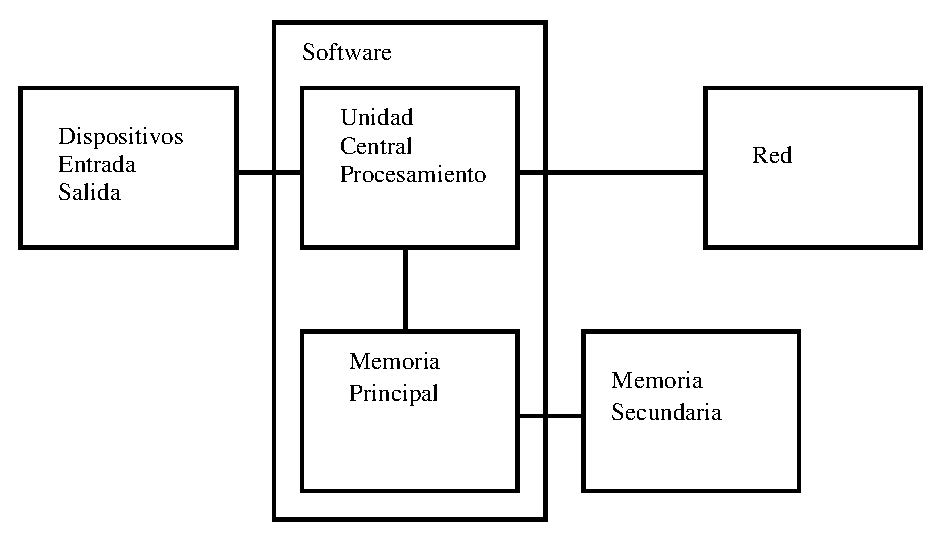
\includegraphics[height=2.50in]{figs2/arch3.eps}}
\afterfig

En este capítulo, comenzaremos a trabajar con la {\bf Memoria Secundaria}
(o ficheros, o archivos).
La memoria secundaria no se borra aunque se interrumpa la corriente.
Incluso, en el caso de una unidad flash USB, los
datos que escribimos desde nuestros programas pueden ser retirados
del sistema y transportados a otro equipo.

En primer lugar nos centraremos en leer y escribir ficheros de texto,
como los que se crean usando un editor de texto cualquiera. Más tarde veremos cómo
trabajar con archivos de bases de datos, que son ficheros binarios diseñados
específicamente para ser leídos y escritos mediante software de manejo de bases de datos.

\section{Apertura de ficheros}
\index{fichero!abrir}
\index{open, función}
\index{función!open}

Cuando se desea leer o escribir en un archivo (nos referimos en el disco duro), primero
debemos {\bf abrir} el fichero. Al abrir el fichero nos comunicamos con el sistema
operativo, que sabe dónde se encuentran almacenados los datos de cada archivo. Cuando se
abre un fichero, se está pidiendo al sistema operativo que lo busque por su nombre
y se asegure de que existe. En este ejemplo, abrimos el fichero
{\tt mbox.txt}, que debería estar guardado en la misma carpeta en la que te
encontrabas cuando iniciaste Python.
Puedes descargar el fichero desde
\url{www.py4inf.com/code/mbox.txt}

\beforeverb
\begin{verbatim}
>>> manf = open('mbox.txt')
>>> print manf
<open file 'mbox.txt', mode 'r' at 0x1005088b0>
\end{verbatim}
\afterverb
%
\index{manejador de fichero}
Si la {\tt apertura} tiene éxito, el sistema operativo nos devuelve un
{\bf manejador de fichero} (file handle). El manejador de fichero no son los datos que
contiene en realidad el archivo, sino que se trata de un ``manejador'' (handle) que se
puede utilizar para leer esos datos. Sólo obtendrás el manejador si el fichero especificado
existe y además dispones de los permisos apropiados para poder leerlo.

\beforefig
\centerline{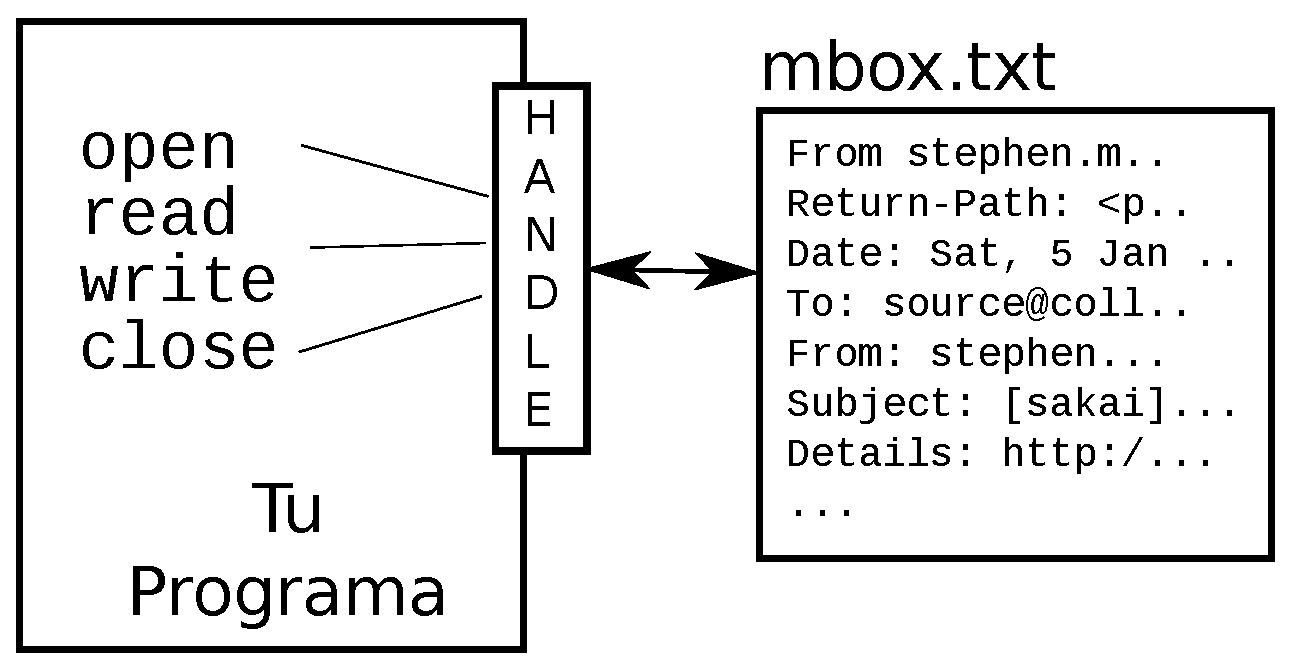
\includegraphics[height=1.75in]{figs2/handle.eps}}
\afterfig

Si el fichero no existe, {\tt open} fallará con un traceback, y no obtendrás
ningún manejador para poder acceder a su contenido:

\beforeverb
\begin{verbatim}
>>> manf = open('stuff.txt')
Traceback (most recent call last):
  File "<stdin>", line 1, in <module>
IOError: [Errno 2] No such file or directory: 'stuff.txt'
\end{verbatim}
\afterverb
%
Más adelante usaremos {\tt try} y {\tt except} para controlar con más
elegancia la situación cuando intentemos abrir un archivo
que no existe.

\section{Ficheros de texto y líneas}

Un fichero de texto puede ser considerado una secuencia de líneas, de igual
modo que una cadena en Python puede ser considerada una secuencia de caracteres.
Por ejemplo, ésta es una muestra de un fichero de texto que guarda la actividad de correos
de varias personas en el equipo de desarrollo de un proyecto de código abierto:

\beforeverb
\begin{alltt}
From stephen.marquard@uct.ac.za Sat Jan  5 09:14:16 2008
Return-Path: <postmaster@collab.sakaiproject.org>
Date: Sat, 5 Jan 2008 09:12:18 -0500
To: source@collab.sakaiproject.org
From: stephen.marquard@uct.ac.za
Subject: [sakai] svn commit: r39772 - content/branches/
Details: http://source.sakaiproject.org/viewsvn/?view=rev\&rev=39772
...
\end{alltt}
\afterverb

El fichero completo de interacciones de correo está disponible en
\url{www.py4inf.com/code/mbox.txt} 
y una versión más reducida se puede encontrar en
\url{www.py4inf.com/code/mbox-short.txt}.
Estos ficheros tienen un formato estándar, diseñado para archivos que contienen
múltiples mensajes de correo. Las líneas que comienzan con
``From '' separan los mensajes, y las líneas que comienzan con
``From:'' son parte de los mensajes.
Para tener más información sobre el formato mbox, consulta
\url{en.wikipedia.org/wiki/Mbox}. 

Para dividir el archivo en líneas, existe un carácter especial que
representa el ``final de línea'', llamado {\bf salto de línea} (newline).

\index{salto de línea}
En Python, el carácter {\bf salto de línea} se representa por barra invertida-n en
las cadenas. A pesar de que parezcan dos caracteres, se
trata en realidad de uno sólo. Cuando revisamos la variable introduciendo
``cosa'' en el intérprete, nos mostrará el \verb"\n" en la cadena,
pero cuando usemos {\tt print} para mostrar la cadena, veremos cómo ésta
aparece dividida en dos líneas por el carácter de salto de línea.

\beforeverb
\begin{verbatim}
>>> cosa = '¡Hola\nMundo!'
>>> cosa
'¡Hola\nMundo!'
>>> print cosa
¡Hola
Mundo!
>>> cosa = 'X\nY'
>>> print cosa
X
Y
>>> len(cosa)
3
\end{verbatim}
\afterverb
%

También puedes observar que la longitud de la cadena \verb"'X\nY'" es de \emph{tres}
caracteres, porque el carácter de salto de línea se cuenta como uno sólo.

De modo que cuando miremos a las líneas de un fichero, tendremos que \emph{imaginarnos}
que existe un carácter especial invisible llamado salto de línea al
final de cada línea, que marca donde termina la misma y comienza la siguiente.

% \beforeverb
% \begin{alltt}
% From stephen.marquard@uct.ac.za Sat Jan  5 09:14:16 2008\verb"\n"\\
% Return-Path: <postmaster@collab.sakaiproject.org>\verb"\n"\\
% Date: Sat, 5 Jan 2008 09:12:18 -0500\verb"\n"\\
% To: source@collab.sakaiproject.org\verb"\n"\\
% From: stephen.marquard@uct.ac.za\verb"\n"\\
% Subject: [sakai] svn commit: r39772 - content/branches/\verb"\n"\\
% Details: http://source.sakaiproject.org/viewsvn/?view=rev\&rev=39772\verb"\n"\\
% ...
% \end{alltt}
% \afterverb

Así que el carácter de salto de línea separa los caracteres
del fichero en líneas.

\section{Lectura de ficheros}

\index{fichero!lectura}
\index{contador}
A pesar de que el {\bf manejador de fichero} no contiene los datos del archivo,
es bastante fácil construir un bucle {\tt for} para ir leyendo
y contabilizando cada una de las líneas de un fichero:

\beforeverb
\begin{verbatim}
manf = open('mbox.txt')
contador = 0
for linea in manf:
    contador = contador + 1
print 'Líneas contabilizadas:', contador

python open.py 
Line Count: 132045
\end{verbatim}
\afterverb
%
Podemos usar el manejador del fichero como una secuencia en nuestro bucle {\tt for}.
El bucle {\tt for} simplemente cuenta el número de líneas del
fichero y lo muestra en pantalla. La traducción aproximada del bucle for
al español es: ``para cada línea del fichero representado por este
manejador, añade una unidad a la variable {\tt contador}''.

La razón de que la función {\tt open} no lea el archivo completo
es que el fichero puede ser bastante extenso, con muchos gigabytes de datos.
La sentencia {\tt open} emplea la misma cantidad de tiempo independientemente del
tamaño del archivo. En realidad es el bucle {\tt for} el que hace que
los datos sean leídos desde el fichero.

Cuando el archivo se lee de este modo, usando un bucle {\tt for}, Python
se encarga de dividir los datos del fichero en líneas independientes, usando
el carácter de salto de línea. Python lee cada línea hasta el
salto de línea e incluye
el propio salto de línea como último carácter en la variable {\tt linea} para
cada iteración del bucle {\tt for}.

Debido a que el bucle {\tt for} lee los datos línea a línea, puede
leer y contar las líneas de forma eficiente en ficheros muy extensos sin
agotar la memoria de almacenamiento de datos. El programa anterior puede
contar las líneas de ficheros de cualquier tamaño usando muy poca memoria,
ya que cada línea es leída, contada y luego descartada.

Si sabes que el fichero es relativamente pequeño comparado con el tamaño de
tu memoria principal, puedes leer el fichero completo en una cadena
usando el método {\tt read} sobre el manejador del fichero.

\beforeverb
\begin{verbatim}
>>> manf = open('mbox-short.txt')
>>> ent = manf.read()
>>> print len(ent)
94626
>>> print ent[:20]
From stephen.marquar
\end{verbatim}
\afterverb
%
En este ejemplo, el contenido completo (los 94.626 caracteres)
del fichero {\tt mbox-short.txt} se leen directamente dentro de la variable
{\tt ent}. Usamos luego rebanado de cadenas para imprimir en pantalla
los primeros 20 caracteres de la cadena de datos almacenada en {\tt inp}.

Cuando el archivo se lee de esta manera, todos los caracteres incluyendo
las líneas completas y los saltos de línea forman parte de una gran cadena
que se guarda en la variable {\bf ent}.
Recuerda que esta forma de uso de la función {\tt open} sólo debe utilizarse
si el fichero de datos cabe holgadamente en la memoria principal
de tu ordenador.

Si el fichero es demasiado grande para caber en la memoria principal, deberías
hacer que tu programa leyera el archivo en bloques, usando un bucle
{\tt for} o {\tt while}.

\section{Búsqueda dentro de un fichero}

Cuando se buscan datos dentro de un fichero, un
patrón muy común consiste en ir leyendo el archivo completo, ignorando
la mayoría de las líneas y procesando únicamente aquellas que cumplen alguna condición
particular. Es posible combinar ese patrón de lectura de ficheros con los métodos de cadena
para construir un mecanismo simple de búsqueda.

\index{filtrado, patrón}
\index{patrón!de filtrado}
Por ejemplo, si queremos leer un fichero y mostrar unicamente aquellas líneas
que comienzan con el prefijo ``From:'', podemos usar el
método de cadena {\bf startwith} para seleccionar solamente aquellas líneas con
el prefijo deseado:

\beforeverb
\begin{verbatim}
manf = open('mbox-short.txt')
for linea in manf:
    if linea.startswith('From:') :
        print linea
\end{verbatim}
\afterverb
%
Cuando se hace funcionar el programa, obtenemos la siguiente salida:

\beforeverb
\begin{verbatim}
From: stephen.marquard@uct.ac.za

From: louis@media.berkeley.edu

From: zqian@umich.edu

From: rjlowe@iupui.edu
...
\end{verbatim}
\afterverb
%
La salida parece ser correcta, ya que las únicas líneas que vemos son aquellas
que comienzan por ``From:''. Pero, ¿por qué estamos viendo líneas extra
vacías? Esto se debe al carácter invisible de {\bf salto de línea}.
Cada una de las líneas termina con un salto de línea, de modo que la sentencia
{\tt print} imprime la cadena que está en la variable {\bf linea} y que
incluye un salto de línea, y a continuación {\tt print} añade \emph{otro} salto de línea,
cuyo resultado es el efecto de doble espaciado que podemos ver.

Podríamos usar rebanado de líneas para imprimir todo menos el último carácter, pero
un enfoque más sencillo consiste en usar el método {\bf rstrip}, que retira
los espacios en blanco de la parte derecha de una cadena, como se muestra a continuación:

\beforeverb
\begin{verbatim}
manf = open('mbox-short.txt')
for linea in manf:
    linea = linea.rstrip()
    if linea.startswith('From:') :
        print linea
\end{verbatim}
\afterverb
%
Cuando hacemos funcionar el programa, obtenemos la siguiente salida:

\beforeverb
\begin{verbatim}
From: stephen.marquard@uct.ac.za
From: louis@media.berkeley.edu
From: zqian@umich.edu
From: rjlowe@iupui.edu
From: zqian@umich.edu
From: rjlowe@iupui.edu
From: cwen@iupui.edu
...
\end{verbatim}
\afterverb
%
A medida que los programas de procesado de archivos se van volviendo más complejos, es posible
que queramos estructurar los bucles de búsqueda usando {\tt continue}. La idea básica
del bucle de búsqueda es que estamos localizando líneas ``interesantes''
y saltando eficazmente aquellas que ``no nos interesan''. Y a continuación, cuando
encontramos una línea interesante, hacemos algo con esa línea.

Podemos estructurar el bucle para usar ese
diseño y saltar las líneas que no nos interesan, de este modo:

\beforeverb
\begin{verbatim}
manf = open('mbox-short.txt')
for linea in manf:
    linea = linea.rstrip()
    # Saltar 'líneas que no nos interesan'
    if not linea.startswith('From:') :
        continue
    # Procesar nuestra línea 'interesante'
    print linea
\end{verbatim}
\afterverb
%
La salida del programa es la misma. Traduciendo, las
líneas que no nos interesan son aquellas que no comienzan
por ``From:'', de modo que las saltamos usando {\tt continue}.
En cambio las líneas ``interesantes'' (es decir, aquellas que comienzan por ``From:''),
procedemos a procesarlas.

Podemos usar el método {\tt find} para simular una búsqueda como la de
un editor que texto, que localice aquellas líneas que contengan la cadena buscada
en cualquier punto de las mismas.
Dado que {\tt find} comprueba la aparición de una cadena dentro de otra
y devuelve la posición de la cadena o -1 si no la ha encontrado,
podemos escribir el bucle siguiente para mostrar aquellas líneas
que contienen la cadena ``@uct.ac.za'' (es decir, las que proceden de la Universidad
de Cape Town en Sudáfrica):

\beforeverb
\begin{verbatim}
manf = open('mbox-short.txt')
for linea in manf:
    linea = linea.rstrip()
    if linea.find('@uct.ac.za') == -1 : 
        continue
    print linea
\end{verbatim}
\afterverb
%
Que produce la siguiente salida:

\beforeverb
\begin{verbatim}
From stephen.marquard@uct.ac.za Sat Jan  5 09:14:16 2008
X-Authentication-Warning: set sender to stephen.marquard@uct.ac.za using -f
From: stephen.marquard@uct.ac.za
Author: stephen.marquard@uct.ac.za
From david.horwitz@uct.ac.za Fri Jan  4 07:02:32 2008
X-Authentication-Warning: set sender to david.horwitz@uct.ac.za using -f
From: david.horwitz@uct.ac.za
Author: david.horwitz@uct.ac.za
...
\end{verbatim}
\afterverb
%

\section{Permitir al usuario elegir el nombre del fichero}

Lo más probable es que no nos apetezca editar nuestro código Python
cada vez que queramos procesar un archivo diferente. Sería
más útil pedir al usuario que introdujera una cadena con el nombre del fichero
cada vez que el programa funcione, de modo que pueda usar nuestro
programa sobre ficheros diferentes sin tener que cambiar el código Python.

Esto es bastante sencillo de hacer, pidiendo el nombre del fichero al
usuario mediante el uso de \verb"raw_input", como se muestra a continuación:

\beforeverb
\begin{verbatim}
nombref = raw_input('Introduce el nombre del fichero: ')
manf = open(nombref)
contador = 0
for linea in manf:
    if linea.startswith('Subject:') :
        contador = contador + 1
print 'Hay', contador, 'líneas subject en', nombref
\end{verbatim}
\afterverb
%
Pedimos el nombre del fichero al usuario, lo guardamos en una variable
llamada {\tt nombref} y abrimos ese fichero. Ahora ya podemos hacer funcionar
el programa repetidamente con distintos ficheros.

\beforeverb
\begin{verbatim}
python search6.py 
Introduce el nombre del fichero: mbox.txt
Hay 1797 líneas subject en mbox.txt

python search6.py 
Introduce el nombre del fichero: mbox-short.txt
Hay 27 líneas subject en mbox-short.txt
\end{verbatim}
\afterverb
%
Antes de asomarte a la siguiente sección, échale un vistazo al programa anterior
y pregúntate a ti mismo: ``¿Qué podría ir mal aquí?'', o ``¿Qué podría hacer
nuestro simpático usuario que provoque que nuestro bonito programita
termine sin gracia, con un tracebak, haciéndonos parecer menos geniales
ante los usuarios?

\section{Uso de {\tt try, except,} y {\tt open}}

Te avisé que no te asomases. Esta es tu última oportunidad.

¿Qué ocurre si nuestro usuario escribe algo que no es un nombre de fichero?

\beforeverb
\begin{verbatim}
python search6.py 
Introduce el nombre del fichero: perdido.txt
Traceback (most recent call last):
  File "search6.py", line 2, in <module>
    manf = open(nombref)
IOError: [Errno 2] No such file or directory: 'perdido.txt'

python search6.py 
Introduce el nombre del fichero: na na boo boo
Traceback (most recent call last):
  File "search6.py", line 2, in <module>
    manf = open(nombref)
IOError: [Errno 2] No such file or directory: 'na na boo boo'
\end{verbatim}
\afterverb
%
No te rías, los usuarios harán de vez en cuando todo lo que puedan por estropear
tus programas---ya sea a propósito o con malas intenciones.
De hecho, una parte importante de cualquier equipo de desarrollo de software
es una persona o grupo llamado {\bf Controlador de Calidad}
(o QA por sus siglas en inglés), cuyo trabajo principal es hacer las cosas más disparatadas
posibles para intentar hacer fallar el software que el programador ha creado.

\index{Controlador de Calidad}
\index{QA}
El equipo de QA es el responsable de encontrar los defectos en los programas antes
de que éstos se entreguen a los usuarios finales, que pueden estar comprando el
software o pagando su salario a los que escriben el software. De modo que el equipo QA
es el mejor amigo del programador.

\index{try, sentencia}
\index{sentencia!try}
\index{open, función}
\index{función!open}
\index{exception!IOError}
\index{IOError}
Así que ahora que hemos visto el defecto en el programa, podemos solucionarlo
de forma elegante usando la estructura {\tt try}/{\tt except}. Debemos asumir que la llamada
a {\tt open} puede fallar y añadir código de recuperación para ese fallo,
como se muestra a continuación:

\beforeverb
\begin{verbatim}
nombref = raw_input('Introduce el nombre del fichero: ')
try:
    manf = open(nombref)
except:
    print 'No se pudo abrir el fichero:', nombref
    exit()

contador = 0
for linea in manf:
    if linea.startswith('Subject:') : 
        contador = contador + 1
print 'Hay', contador, 'líneas subject en', nombref
\end{verbatim}
\afterverb
%
La función {\tt exit} hace finalizar el programa. Se trata de una función
que llamamos sin retorno. Ahora cuando el usuario (o
el equipo de QA) escriba tonterías o nombres de archivo incorrectos,
los ``capturaremos'' y recuperaremos el control del programa con elegancia:

\beforeverb
\begin{verbatim}
python search7.py
Introduce el nombre del fichero: mbox.txt
Hay 1797 líneas subject en mbox.txt

python search7.py
Introduce el nombre del fichero: na na boo boo
No se pudo abrir el fichero: na na boo boo
\end{verbatim}
\afterverb
%
\index{Pythónico}
La protección de la llamada a {\tt open} es un buen ejemplo
del uso correcto de {\tt try}
y {\tt except} en un programa Python. Se utiliza el término
``Pythónico'' cuando estamos haciendo algo al ``modo
Python''. Podríamos decir que el ejemplo de arriba es
el modo Pythónico de abrir un archivo.

Una vez que adquieras más soltura en Python, puedes intercambiar
opiniones con otros programadores de Python para decidir
cual de dos soluciones equivalente para un problema es
``más Pythónica''. La ambición de ser ``más Pythónico''
capta la idea de que programar es parte ingeniería
y parte arte. No siempre estamos interesados únicamente
en hacer que algo funcione sin más, también queremos que nuestra solución
sea elegante y que sea apreciada por su elegancia
por nuestros colegas.


\section{Escritura en ficheros}

\index{fichero!escritura}

Para escribir en un fichero, debes abrirlo usando el modo
\verb"'w'" (de {\tt write}) como segundo parámetro:

\beforeverb
\begin{verbatim}
>>> fsal = open('salida.txt', 'w')
>>> print fsal
<open file 'salida.txt', mode 'w' at 0xb7eb2410>
\end{verbatim}
\afterverb
%
Si el fichero ya existe, abrirlo en modo escritura eliminará
los datos antiguos y lo dejará completamente vacío, ¡así que ten cuidado!
Si el fichero no existe, se creará nuevo.

El método {\tt write} del objeto manejador del fichero
pone datos dentro del archivo.

\beforeverb
\begin{verbatim}
>>> linea1 = "Aquí está el zarzo,\n"
>>> fsal.write(linea1)
\end{verbatim}
\afterverb
%
\index{salto de línea}
El objeto fichero también realiza el seguimiento de la posición dentro del fichero, de modo
que si se llama a {\tt write} otra vez, añadirá los datos nuevos al final del archivo.

Deberemos asegurarnos de gestionar los finales de las líneas mientras
escribimos en el fichero, insertando explícitamente el carácter de salto
cuando queramos terminar una línea. La sentencia {\tt print}
añade un salto de línea automáticamente, pero el método
{\tt write} no lo hace a menos que se lo especifiquemos.

\beforeverb
\begin{verbatim}
>>> linea2 = 'el símbolo de nuestra tierra.\n'
>>> fsal.write(linea2)
\end{verbatim}
\afterverb
%
Cuando hayas terminado de escribir, debes cerrar el fichero
para asegurarte de que hasta el último bit de datos se escriba
físicamente en el disco, de modo que no se pierda si la corriente se interrumpe.

\beforeverb
\begin{verbatim}
>>> fsal.close()
\end{verbatim}
\afterverb
%
También se pueden cerrar los ficheros que se han abierto en modo lectura,
pero no es necesario que seamos muy estrictos con ello si solamente
estamos abriendo unos pocos archivos, ya que Python se asegura de que
todos los ficheros queden cerrados cuando el programa termina. En cambio, en el caso
de que estemos escribiendo ficheros, deberemos cerrarlos explícitamente
para no dejar nada al azar.

\index{close, método}
\index{método!close}


\section{Depuración}

\index{depuración}
\index{espacio en blanco}

Cuando estés leyendo y escribiendo archivos, puedes tener problemas
con los espacios en blanco. Estos errores pueden ser difíciles de depurar porque los espacios,
tabulaciones y saltos de línea normalmente son invisibles:

\beforeverb
\begin{verbatim}
>>> s = '1 2\t 3\n 4'
>>> print s
1 2	 3
 4
\end{verbatim}
\afterverb

\index{repr, función}
\index{función!repr}
\index{cadena!representación de}

La función incorporada {\tt repr} puede ayudarnos. Toma cualquier objeto como
argumento y devuelve una representación de cadena del objeto. En el caso
de las cadenas, representa los caracteres en blanco
con secuencias de barras invertidas:

\beforeverb
\begin{verbatim}
>>> print repr(s)
'1 2\t 3\n 4'
\end{verbatim}
\afterverb

Esto puede resultarnos de utilidad a la hora de depurar.

Otro problema que puedes tener se debe a que los distintos sistemas
utilizan caracteres diferentes para indicar el final de una línea. Algunos
sistemas usan un salto de línea, representado por \verb"\n". Otros
usan un carácter de retorno, representado por \verb"\r". Otros usan ambos.
Si trasladas ficheros entre sistemas diferentes, esas inconsistencias
pueden causar problemas.

\index{final de línea, carácter de}

En la mayoría de los sistemas, existen aplicaciones para convertir de un
formato a otro. Puedes encontrarlos (y leer más acerca de este
problema) en \url{wikipedia.org/wiki/Newline}.  O, por supuesto, puedes
escribir tu propio programa.

% TBD - ¿¿¿No se ocupa Python de esto por nosotros????

\section{Glosario}

\begin{description}

\item[capturar (catch):] Evitar que una excepción haga terminar
un programa, usando las sentencias {\tt try} y {\tt except}.
\index{catch}
\index{capturar}

\item[Controlador de Calidad:] Una persona o equipo centrada en asegurar
la calidad del conjunto en un producto software.
Sus siglas en inglés son QA (Quality Assurance). El QA se encarga normalmente
de probar un producto e identificar sus problemas antes de que éste
sea lanzado.
\index{Controlador de Calidad}
\index{QA}

\item[fichero de texto:] Una secuencia de caracteres almacenados en un
medio de almacenamiento permanente, como un disco duro.
\index{fichero!de texto}

\item[Pythónico:] Una técnica que funciona de forma elegante en Python.
``Usar try y except y es la forma \emph{Pythónica} de restablecer un programa en
caso de intentar abrir archivos que no existen''.
\index{Pythónico}

\item[salto de línea:] Un carácter especial que se utiliza en los archivos y cadenas
para indicar el final de una línea.
\index{salto de línea}

\end{description}


\section{Ejercicios}

\begin{ex}
Escribe un programa que lea un fichero e imprima en pantalla su contenido
(línea a línea), todo en mayúsculas. La ejecución del programa debería
ser algo similar a esto:

\beforeverb
\begin{verbatim}
python shout.py
Introduce el nombre del fichero: mbox-short.txt
FROM STEPHEN.MARQUARD@UCT.AC.ZA SAT JAN  5 09:14:16 2008
RETURN-PATH: <POSTMASTER@COLLAB.SAKAIPROJECT.ORG>
RECEIVED: FROM MURDER (MAIL.UMICH.EDU [141.211.14.90])
	 BY FRANKENSTEIN.MAIL.UMICH.EDU (CYRUS V2.3.8) WITH LMTPA;
	 SAT, 05 JAN 2008 09:14:16 -0500
\end{verbatim}
\afterverb
%
Puedes descargar el fichero desde
\url{www.py4inf.com/code/mbox-short.txt}
\end{ex}

\begin{ex}
Escribe un programa
que pida el nombre de un fichero y después lea ese fichero,
buscando líneas que tengan la forma:

\beforeverb
\begin{alltt}
X-DSPAM-Confidence: {\bf 0.8475}
\end{alltt}
\afterverb

Cuando encuentres una línea que comienza por
``X-DSPAM-Confidence:'', separa esa línea para extraer
el número en punto flotante que figure en ella. Cuenta esas línea y
calcula también el total de los valores de probabilidad de spam (spam confidence)
de estas líneas. Cuando alcances el final del archivo, muestra en pantalla
el valor medio de probabilidad de spam.

\beforeverb
\begin{verbatim}
Introduce el nombre del fichero: mbox.txt
Valor medio de probabilidad de spam: 0.894128046745

Introduce el nombre del fichero: mbox-short.txt
Valor medio de probabilidad de spam: 0.750718518519
\end{verbatim}
\afterverb
%
Prueba tu programa con los archivos {\tt mbox.txt} y {\tt mbox-short.txt}.
\end{ex}


\begin{ex}
Algunas veces, cuando los programadores se aburren o quieren divertirse un poco,
añaden inofensivos {\bf Huevos de Pascua (Easter Egg)} en sus programas
(\url{es.wikipedia.org/wiki/Huevo_de_pascua_(virtual)}). Modifica el programa
que pide al usuario el nombre del fichero para que imprima un mensaje
divertido cuando el usuario escriba el nombre exacto ``na na boo boo''.
El programa debe comportarse normalmente con todos los demás ficheros,
tanto los que existan como los que no. A continuación una muestra de la ejecución
del programa:

\beforeverb
\begin{verbatim}
python egg.py 
Introduce el nombre del fichero:  mbox.txt
Hay 1797 líneas subject en mbox.txt

python egg.py 
Introduce el nombre del fichero:  missing.tyxt
No se pudo abrir el fichero: missing.tyxt

python egg.py 
Introduce el nombre del fichero: na na boo boo
NA NA BOO BOO PARA TI - ¡Has sido un niño malo!
\end{verbatim}
\afterverb
%
No te estamos animando a poner Huevos de Pascua en tus
programa---se trata sólo de un ejercicio.

\end{ex}
% LaTeX source for ``Python for Informatics: Exploring Information''
% Copyright (c)  2010-  Charles R. Severance, All Rights Reserved

\chapter{Listas}

\index{lista}
\index{tipo!list}


\section{Una lista es una secuencia}

Al igual que una cadena, una {\bf lista} es una secuencia de valores. En una cadena, los
valores son caracteres; en una lista, pueden ser de cualquier tipo. Los valores en las
listas reciben el nombre de {\bf elementos}, o a veces {\bf artículos}.

\index{elemento}
\index{secuencia}
\index{artículo}

Hay varios modos de crear una lista nueva; el más simple
consiste en encerrar los elementos entre corchetes (\verb"[" y \verb"]"):

\beforeverb
\begin{verbatim}
[10, 20, 30, 40]
['rana crujiente', 'vejiga de carnero', 'vómito de alondra']
\end{verbatim}
\afterverb
%
El primer ejemplo es una lista de cuatro enteros. El segundo es una lista
de tres cadenas. Los elementos en una lista no tienen por qué ser todos del mismo tipo.
La lista siguiente contiene una cadena, un flotante, un entero y
(¡ahí va!) otra lista:

\beforeverb
\begin{verbatim}
['spam', 2.0, 5, [10, 20]]
\end{verbatim}
\afterverb
%
Una lista dentro de otra se dice que está {\bf anidada}.

\index{anidada, lista}
\index{lista!anidada}

Una lista que no contiene elementos recibe el nombre
de lista vacía; se puede crear una simplemente
con unos corchetes vacíos, \verb"[]".

\index{vacía, lista}
\index{lista!vacía}

Como es lógico, puedes asignar listas de valores a variables:

\beforeverb
\begin{verbatim}
>>> quesos = ['Cheddar', 'Edam', 'Gouda']
>>> numeros = [17, 123]
>>> vacia = []
>>> print quesos, numeros, vacia
['Cheddar', 'Edam', 'Gouda'] [17, 123] []
\end{verbatim}
\afterverb
%

\index{asignación}

\section{Las listas son mutables}

\index{lista!elemento}
\index{accesso}
\index{índice}
\index{corchete, operador}
\index{operador!corchete}

La sintaxis para acceder a los elementos de una lista es la misma que
para acceder a los caracteres de una cadena---el operador corchete. La
expresión dentro de los corchetes especifica el índice. Recuerda que los
índices comienzan por 0:

\beforeverb
\begin{verbatim}
>>> print quesos[0]
Cheddar
\end{verbatim}
\afterverb
%
A diferencia de las cadenas, las listas son mutables (pueden mutar), porque puedes cambiar el orden
de los elementos o reasignar un elemento dentro de la lista.
Cuando el operador corchete aparece en el lado izquierdo de una asignación,
éste identifica el elemento de la lista que será asignado.

\index{mutabilidad}

\beforeverb
\begin{verbatim}
>>> numeros = [17, 123]
>>> numeros[1] = 5
>>> print numeros
[17, 5]
\end{verbatim}
\afterverb
%
El elemento de {\tt numeros} cuyo índice es uno, que
antes era 123, es ahora 5.

\index{índice!comienza en cero}
\index{cero, índice comienza en}

Puedes pensar en una lista como una relación entre índices y
elementos. Esta relación recibe el nombre de {\bf mapeo o direccionamiento}; cada índice
``dirige a'' uno de los elementos.


\index{elemento!asignación}
\index{asignación!elemento}

Los índices de una lista funcionan del mismo modo que los índices de una cadena:

\begin{itemize}

\item Cualquier expresión entera puede ser utilizada como índice.

\item Si se intenta leer o escribir un elemento que no existe,
se obtiene un {\tt IndexError}.

\index{exception!IndexError}
\index{IndexError}

\item Si un índice tiene un valor negativo, contará hacia atrás desde
el final de la lista.

\end{itemize}

\index{lista!índice}


\index{lista!pertenencia}
\index{pertenencia!lista}
\index{in, operador}
\index{operador!in}

El operador {\tt in} también funciona con las listas.

\beforeverb
\begin{verbatim}
>>> quesos = ['Cheddar', 'Edam', 'Gouda']
>>> 'Edam' in quesos
True
>>> 'Brie' in quesos
False
\end{verbatim}
\afterverb


\section{Recorrer una lista}
\index{lista!recorrido}
\index{recorrido!lista}
\index{for, bucle}
\index{bucle!for}
\index{sentencia!for}

El modo más habitual de recorrer los elementos de una lista es
con un bucle {\tt for}. La sintaxis es la misma que para las cadenas:

\beforeverb
\begin{verbatim}
for queso in quesos:
    print queso
\end{verbatim}
\afterverb
%
Esto funciona correctamente si sólo se necesita leer los elementos de la
lista. Pero si quieres escribir o modificar los elementos,
necesitarás los índices. Un modo habitual de hacerlo consiste en combinar
las funciones {\tt range} y {\tt len}:

\index{iteración!con índices}
\index{índice!iterando con}

\beforeverb
\begin{verbatim}
for i in range(len(numeros)):
    numeros[i] = numeros[i] * 2
\end{verbatim}
\afterverb
%
Este bucle recorre la lista y actualiza cada elemento. {\tt len}
devuelve el número de elementos de la lista. {\tt range} devuelve
una lista de índices desde 0 hasta $n-1$, donde $n$ es la longitud de
la lista. Cada vez que atravesamos el bucle, {\tt i} obtiene el índice
del elemento siguiente. La sentencia de asignación en el cuerpo usa
{\tt i} para leer el valor antiguo del elemento y asignarle el
valor nuevo.

\index{elemento, actualizar}
\index{actualizar!elemento}

Un bucle {\tt for} aplicado a una lista vacía no ejecuta nunca el código contenido en su cuerpo:

\beforeverb
\begin{verbatim}
for x in vacia:
    print 'Esto nunca ocurrirá.'
\end{verbatim}
\afterverb
%
A pesar de que una lista puede contener otra, la lista
anidada sólo cuenta como un único elemento. La longitud de esta lista
es cuatro:

\index{anidada, lista}
\index{lista!anidada}

\beforeverb
\begin{verbatim}
['spam', 1, ['Brie', 'Roquefort', 'Pol le Veq'], [1, 2, 3]]
\end{verbatim}
\afterverb



\section{Operaciones con listas}
\index{lista!operación}

El operador {\tt +} concatena listas:

\index{concatenación!lista}
\index{lista!concatenación}

\beforeverb
\begin{verbatim}
>>> a = [1, 2, 3]
>>> b = [4, 5, 6]
>>> c = a + b
>>> print c
[1, 2, 3, 4, 5, 6]
\end{verbatim}
\afterverb
%
De forma similar, el operador {\tt *} repite una lista el número especificado de veces:

\index{repeticion!lista}
\index{lista!repetición}

\beforeverb
\begin{verbatim}
>>> [0] * 4
[0, 0, 0, 0]
>>> [1, 2, 3] * 3
[1, 2, 3, 1, 2, 3, 1, 2, 3]
\end{verbatim}
\afterverb
%
El primer ejemplo repite {\tt [0]} cuatro veces. El segundo,
repite la lista {\tt [1, 2, 3]} tres veces.


\section{Rebanado de listas}

\index{rebanada!operador}
\index{operador!rebanada}
\index{índice!rebanada}
\index{lista!rebanada}
\index{rebanada!lista}
\index{slice!lista}
\index{lista!slice}

El operador de rebanada ({\tt slice}) también funciona en listas:

\beforeverb
\begin{verbatim}
>>> t = ['a', 'b', 'c', 'd', 'e', 'f']
>>> t[1:3]
['b', 'c']
>>> t[:4]
['a', 'b', 'c', 'd']
>>> t[3:]
['d', 'e', 'f']
\end{verbatim}
\afterverb
%
Si omites el primer índice, la rebanada comenzará al principio.
Si omites el segundo, la rebanada llegará hasta el final. De modo que
si omites ambos, la rebanada será una copia de la lista completa.

\index{lista!copiar}
\index{rebanada!copiar}
\index{copiar!rebanada}

\beforeverb
\begin{verbatim}
>>> t[:]
['a', 'b', 'c', 'd', 'e', 'f']
\end{verbatim}
\afterverb
%
Como las listas son mutables, a menudo resultará útil hacer una copia
antes de realizar operaciones que dupliquen elementos, los hagan rotar o mutilen
de algún modo esas listas.

\index{mutabilidad}

Un operador de rebanada en la parte izquierda de una asignación
puede modificar múltiples elementos:

\index{rebanada!actualizar}
\index{actualizar!rebanada}

\beforeverb
\begin{verbatim}
>>> t = ['a', 'b', 'c', 'd', 'e', 'f']
>>> t[1:3] = ['x', 'y']
>>> print t
['a', 'x', 'y', 'd', 'e', 'f']
\end{verbatim}
\afterverb
%

\section{Métodos de listas}

\index{lista!métodos}
\index{métodos!lista}

Python proporciona varios métodos que operan con listas. Por ejemplo,
{\tt append} añade un nuevo elemento al final de una lista:

\index{append, método}
\index{método!append}

\beforeverb
\begin{verbatim}
>>> t = ['a', 'b', 'c']
>>> t.append('d')
>>> print t
['a', 'b', 'c', 'd']
\end{verbatim}
\afterverb
%
{\tt extend} toma una lista como argumento y añade al final de la actual
todos sus elementos

\index{extend, método}
\index{método!extend}

\beforeverb
\begin{verbatim}
>>> t1 = ['a', 'b', 'c']
>>> t2 = ['d', 'e']
>>> t1.extend(t2)
>>> print t1
['a', 'b', 'c', 'd', 'e']
\end{verbatim}
\afterverb
%
En este ejemplo, {\tt t2} no se modifica.

{\tt sort} ordena los elementos de una lista de menor a mayor:

\index{sort, método}
\index{método!sort}

\beforeverb
\begin{verbatim}
>>> t = ['d', 'c', 'e', 'b', 'a']
>>> t.sort()
>>> print t
['a', 'b', 'c', 'd', 'e']
\end{verbatim}
\afterverb
%
La mayoría de los métodos de lista no devuelven nada; modifican la lista y devuelven {\tt None}.
Si escribes por accidente {\tt t = t.sort()}, seguro que te sientes defraudado
por el resultado.

\index{estéril, método}
\index{método!estéril}
\index{None, valor especial}
\index{valor especial!None}

\section{Borrado de elementos}

\index{borrado de elemento}
\index{borrado, elemento de lista}

Hay varias formas de borrar elementos de una lista. Si conoces
el índice del elemento que quieres eliminar, puedes usar
{\tt pop}:

\index{pop, método}
\index{método!pop}

\beforeverb
\begin{verbatim}
>>> t = ['a', 'b', 'c']
>>> x = t.pop(1)
>>> print t
['a', 'c']
>>> print x
b
\end{verbatim}
\afterverb
%
{\tt pop} modifica la lista y devuelve el elemento que ha sido eliminado.
Si no le proporcionas un índice, borra y devuelve el
último elemento.

Si no necesitas el valor eliminado, puedes usar el operador
{\tt del}:

\index{del, operador}
\index{operador!del}

\beforeverb
\begin{verbatim}
>>> t = ['a', 'b', 'c']
>>> del t[1]
>>> print t
['a', 'c']
\end{verbatim}
\afterverb
%

Si conoces el elemento que quieres eliminar (pero no su índice), puedes
usar {\tt remove}:

\index{remove, método}
\index{método!remove}

\beforeverb
\begin{verbatim}
>>> t = ['a', 'b', 'c']
>>> t.remove('b')
>>> print t
['a', 'c']
\end{verbatim}
\afterverb
%
El valor que devuelve {\tt remove} es {\tt None}.

\index{None, valor especial}
\index{valor especial!None}

Para eliminar más de un elemento, puedes usar {\tt del} con
un índice de rebanada:

\beforeverb
\begin{verbatim}
>>> t = ['a', 'b', 'c', 'd', 'e', 'f']
>>> del t[1:5]
>>> print t
['a', 'f']
\end{verbatim}
\afterverb
%
Como de costumbre, el método de rebanada selecciona todos los elementos hasta (pero
sin incluir) el segundo índice.

\section{Listas y funciones}

Hay varias funciones internas que pueden utilizarse en las listas
y que nos permiten buscar rápidamente a través de ellas
sin tener que escribir nuestros propios bucles:

\beforeverb
\begin{verbatim}
>>> nums = [3, 41, 12, 9, 74, 15]
>>> print len(nums)
6
>>> print max(nums)
74
>>> print min(nums)
3
>>> print sum(nums)
154
>>> print sum(nums)/len(nums)
25
\end{verbatim}
\afterverb
%
La función {\tt sum()} solamente funciona cuando los elementos de la lista son números.
Las otras funciones ({\tt max()}, {\tt len()}, etc.) funcionan también con listas
de cadenas y otros tipos que se puedan comparar.

Podemos reescribir un programa anterior que calculaba la media de
varios números introducidos por el usuario, usando ahora una lista.

Primero, el programa que calculaba la media sin usar listas:

\beforeverb
\begin{verbatim}
total = 0
contador = 0
while ( True ) :
    ent = raw_input('Introduzca un número: ')
    if ent == 'fin' : break
    valor = float(ent)
    total = total + valor
    contador = contador + 1

media = total / contador
print 'Media:', media
\end{verbatim}
\afterverb
%
En este programa, tenemos las variables {\tt contador} y {\tt total}
para almacenar la cantidad y el total actual de los números del usuario
según éste los va introduciendo.

Podemos simplemente guardar cada número que el usuario introduzca
y usar las funciones internas para calcular la suma y la cantidad
de números introducidos al final.

\beforeverb
\begin{verbatim}
listnum = list()
while ( True ) :
    ent = raw_input('Introduzca un número: ')
    if ent == 'fin' : break
    valor = float(ent)
    listnum.append(valor)

media = sum(listnum) / len(listnum)
print 'Media:', media
\end{verbatim}
\afterverb
%
Creamos una lista vacía antes de que el bucle comience, y luego cada vez
que tenemos un número lo añadimos a la lista. Al final del
programa, simplemente calculamos la suma de los números de la
lista y lo dividimos por la cantidad de números,
para obtener la media.

\section{Listas y cadenas}

\index{lista}
\index{cadena}
\index{secuencia}

Una cadena es una secuencia de caracteres y una lista es una secuencia
de valores, pero una lista de caracteres no es lo mismo que una
cadena. Para convertir desde una cadena a una lista de caracteres,
se puede usar la función {\tt list}:

\index{lista!función}
\index{función!list}

\beforeverb
\begin{verbatim}
>>> s = 'spam'
>>> t = list(s)
>>> print t
['s', 'p', 'a', 'm']
\end{verbatim}
\afterverb
%
Debido a que {\tt list} es el nombre de una función interna, debes
evitar usarla como nombre de variable. Yo también evito utilizar la letra {\tt l},
porque se parece mucho al número {\tt 1}. Por eso utilizo {\tt t}.

La función {\tt list} divide una cadena en letras individuales. Si
quieres dividir una cadena en palabras, puedes usar el método
{\tt split}:

\index{split, método}
\index{método!split}

\beforeverb
\begin{verbatim}
>>> s = 'suspirando por los fiordos'
>>> t = s.split()
>>> print t
['suspirando', 'por', 'los', 'fiordos']
>>> print t[2]
los
\end{verbatim}
\afterverb
%
Una vez hayas usado {\tt split} para dividir la cadena
en una lista de palabras, se puede utilizar el operador índice
(corchetes) para buscar una palabra concreta en la lista.

Puedes llamar a {\tt split} con
un argumento opcional llamado {\bf delimitador}, que
especifica qué caracteres se deben usar como delimitadores de palabras.
El ejemplo siguiente usa un guión como delimitador:

\index{opcional, argumento}
\index{argumento!opcional}
\index{delimitador}

\beforeverb
\begin{verbatim}
>>> s = 'spam-spam-spam'
>>> delimitador = '-'
>>> s.split(delimitador)
['spam', 'spam', 'spam']
\end{verbatim}
\afterverb
%
{\tt join} es la inversa de {\tt split}. Toma
una lista de cadenas y
concatena sus elementos. {\tt join} es un método de cadena,
de modo que debes invocarlo sobre el delimitador y pasarle
la lista como un parámetro:

\index{join, método}
\index{método!join}
\index{concatenación}

\beforeverb
\begin{verbatim}
>>> t = ['suspirando', 'por', 'los', 'fiordos']
>>> delimitador = ' '
>>> delimitador.join(t)
'suspirando por los fiordos'
\end{verbatim}
\afterverb
%
En caso de que el delimitador sea el carácter espacio,
entonces {\tt join} coloca un espacio entre las palabras. Para concatenar
cadenas sin espacios, puedes usar la cadena vacía,
\verb"''", como delimitador.

\index{cadena!vacía}


\section{Análisis de líneas}

Normalmente, cuando se está leyendo un archivo,
se deseará hacer con las líneas algo más que simplemente
imprimirlas completas en pantalla. A menudo se querrán encontrar
las ``líneas interesantes'' y luego {\bf parsear} (analizar) cada una de ellas
para buscar alguna \emph{parte} importante en su interior. ¿Qué ocurre si queremos
imprimir el día de la semana de aquellas líneas que comienzan por \mbox{``From ''?}

\beforeverb
\begin{alltt}
From stephen.marquard@uct.ac.za {\bf Sat} Jan  5 09:14:16 2008
\end{alltt}
\afterverb

El método {\tt split} es muy efectivo cuando nos enfrentamos con este
tipo de problemas.
Podemos escribir un pequeño programa que busque las líneas que
comiencen por ``From '', extraer las palabras de esas líneas con {\tt split},
y luego imprimir en pantalla la tercera palabra de cada una:

\beforeverb
\begin{verbatim}
manf = open('mbox-short.txt')
for linea in manf:
    linea = linea.rstrip()
    if not linea.startswith('From ') : continue
    palabras = linea.split()
    print palabras[2]
\end{verbatim}
\afterverb
%
Aquí utilizamos también la forma contraída de la sentencia
{\tt if}, de modo que colocamos el {\tt continue} en la
misma línea que el {\tt if}. Esta forma contraída
del {\tt if} opera igual que cuando el
{\tt continue} se coloca en la siguiente línea e indentado.

El programa produce la siguiente salida:

\beforeverb
\begin{verbatim}
Sat
Fri
Fri
Fri
    ...
\end{verbatim}
\afterverb
%
Más adelante, aprenderemos técnicas más sofisticadas para
seleccionar las líneas con las que vamos a trabajar y veremos cómo extraer
esas líneas para encontrar el fragmento exacto de información
que estamos buscando.

\section{Objetos y valores}

\index{objecto}
\index{valor}

Si ejecutamos estas sentencias de asignación:

\beforeverb
\begin{verbatim}
a = 'banana'
b = 'banana'
\end{verbatim}
\afterverb
%
sabemos que {\tt a} y {\tt b} se refieren ambas a una
cadena, pero no sabemos si se refieren a la
\emph{misma} cadena. Hay dos estados posibles:

\index{alias}

\beforefig
\centerline{\includegraphics{figs2/list1.eps}}
\afterfig

En el primer caso, {\tt a} y {\tt b} se refieren a dos objetos diferentes que
tienen el mismo valor. En el segundo, se refieren al mismo
objeto.

\index{is, operador}
\index{operador!is}

Para comprobar si dos variables se refieren al mismo objeto, puedes
usar el operador {\tt is}.

\beforeverb
\begin{verbatim}
>>> a = 'banana'
>>> b = 'banana'
>>> a is b
True
\end{verbatim}
\afterverb
%
En este ejemplo, Python sólo crea un objeto cadena,
y tanto {\tt a} como {\tt b} se refieren a él.

Pero cuando creas dos listas, obtienes dos objetos:

\beforeverb
\begin{verbatim}
>>> a = [1, 2, 3]
>>> b = [1, 2, 3]
>>> a is b
False
\end{verbatim}
\afterverb
%

En este caso podríamos decir que las dos listas son {\bf equivalentes},
porque tienen los mismos elementos, pero no son {\bf idénticas}, porque
no son el mismo objeto. Si dos objetos son idénticos, también
son equivalentes, pero si son equivalentes, no necesariamente
son idénticos.

\index{equivalencia}
\index{identidad}

Hasta ahora, hemos estado usando ``objeto'' y ``valor''
de forma intercambiable, pero es más preciso decir que un objeto tiene
un valor. Si ejecutas {\tt a = [1,2,3]}, {\tt a} se refiere a un objeto
lista cuyo valor es una secuencia particular de elementos. Si otra
lista tiene los mismos elementos, podemos decir que tiene el mismo valor.

\index{objecto}
\index{valor}


\section{Alias}

\index{alias}
\index{referencia!alias}

Si {\tt a} se refiere a un objeto y asignas {\tt b = a},
entonces ambas variables se refieren al mismo objeto:

\beforeverb
\begin{verbatim}
>>> a = [1, 2, 3]
>>> b = a
>>> b is a
True
\end{verbatim}
\afterverb
%

La asociación de una variable con un objeto recibe el nombre de
{\bf referencia}. En este ejemplo, hay dos referencias para el mismo
objeto.

\index{referencia}

Un objeto con más de una referencia tiene más
de un nombre, de modo que decimos que el objeto tiene uno o varios {\bf alias}.

\index{mutabilidad}

Si el objeto con alias es mutable,
los cambios que se hagan en uno de los alias
afectarán al otro:

\beforeverb
\begin{verbatim}
>>> b[0] = 17
>>> print a
[17, 2, 3]
\end{verbatim}
\afterverb
%
A pesar de que este comportamiento puede resultar útil, es también propenso a errores. En general,
resulta más seguro evitar usar alias cuando se está trabajando con objetos
mutables.

\index{inmutabilidad}

Para objetos inmutables, como cadenas, usar alias no resulta tan
problemático. En este ejemplo:

\beforeverb
\begin{verbatim}
a = 'banana'
b = 'banana'
\end{verbatim}
\afterverb
%
casi nunca importa si {\tt a} y {\tt b} se refieren
a la misma cadena o no.


\section{Listas como argumentos}

\index{lista!como argumento}
\index{argumento}
\index{argumento!lista}
\index{referencia}
\index{parámetro}

Cuando se pasa una lista a una función, la función recibe una referencia
de esa lista.
Si la función modifica un parámetro de la lista, el código que la ha llamado también se verá afectado por el cambio.
Por ejemplo, \verb"borra_primer" elimina el primer elemento de una lista:

\beforeverb
\begin{verbatim}
def borra_primer(t):
    del t[0]
\end{verbatim}
\afterverb
%
Y aquí vemos el modo lo hemos usado:

\beforeverb
\begin{verbatim}
>>> letras = ['a', 'b', 'c']
>>> borra_primer(letras)
>>> print letras
['b', 'c']
\end{verbatim}
\afterverb
%
El parámetro {\tt t} y la variable {\tt letras} son
alias para el mismo objeto.

Resulta importante distinguir entre las operaciones que
modifican listas y las operaciones que crean listas nuevas.
Por ejemplo, el método {\tt append} modifica una lista, pero el
operador {\tt +} crea una lista nueva:

\index{append, método}
\index{método!append}
\index{lista!concatenación}
\index{concatenación!lista}

\beforeverb
\begin{verbatim}
>>> t1 = [1, 2]
>>> t2 = t1.append(3)
>>> print t1
[1, 2, 3]
>>> print t2
None

>>> t3 = t1 + [3]
>>> print t3
[1, 2, 3]
>>> t2 is t3
False
\end{verbatim}
\afterverb

Esta diferencia es importante cuando se escriben funciones que
se supone que modificarán listas. Por ejemplo, esta función
\emph{no} borra el primer elemento de una lista:

\beforeverb
\begin{verbatim}
def no_borra_primer(t):
    t = t[1:]              # ¡INCORRECTO!
\end{verbatim}
\afterverb

El operador de rebanada crea una lista nueva y la asignación
hace que {\tt t} se refiera a ella, pero ninguno de ellos tiene ningún efecto
sobre la lista que se ha pasado como argumento.

\index{rebanada!operador}
\index{operador!rebanada}

Una alternativa consiste en escribir una función que cree y
retorne una lista nueva. Por ejemplo,
{\tt cola} devuelve todos los elementos de la lista
excepto el primero:

\beforeverb
\begin{verbatim}
def cola(t):
    return t[1:]
\end{verbatim}
\afterverb
%
Esta función deja la lista original sin modificar.
Aquí está el modo como se usa:

\beforeverb
\begin{verbatim}
>>> letras = ['a', 'b', 'c']
>>> resto = cola(letras)
>>> print resto
['b', 'c']
\end{verbatim}
\afterverb


\begin{ex}

Escribe una función llamada {\tt recorta}, que tome una lista, la
modifique, eliminando los elementos primero y último, y devuelva {\tt None}.

Después escribe una función llamada {\tt centro}, que tome una lista y
devuelva otra que contenga todos los elementos de la original,
menos el primero y el último.

\end{ex}


\section{Depuración}
\index{depuración}

El uso descuidado de las listas (y otros objetos mutables)
puede ocasionar largas horas de depuración. He aquí algunas
trampas comunes y los modos de evitarlas:

\begin{enumerate}

\item No olvides que la mayoría de los métodos de las listas modifican el argumento y
devuelven {\tt None}. Esto es lo opuesto a lo que hacen los métodos de cadena,
que devuelven una cadena nueva y dejan la original inalterada.

Si estás acostumbrado a escribir código con cadenas como éste:

\beforeverb
\begin{verbatim}
palabra = palabra.strip()
\end{verbatim}
\afterverb

Resulta tentador escribir código con listas como éste:

\beforeverb
\begin{verbatim}
t = t.sort()           # ¡INCORRECTO!
\end{verbatim}
\afterverb

\index{sort, método}
\index{método!sort}

Como {\tt sort} devuelve {\tt None}, la operación
siguiente que realices con {\tt t} es probable que falle.

Antes de usar métodos de lista y operadores, deberías leer la
documentación con cuidado y luego probarlos en modo interactivo. Los
métodos y operadores que comparten listas con otras secuencias (como
cadenas) están documentados en
\url{https://docs.python.org/2/library/stdtypes.html#string-methods}.
Los métodos y operadores que sólo se pueden aplicar a secuencias mutables
están documentados en
\url{https://docs.python.org/2/library/stdtypes.html#mutable-sequence-types}.


\item Elige un estilo y ajústate a él.
\index{estilo}

Parte del problema con las listas es que hay demasiados
modos de hacer las cosas. Por ejemplo, para eliminar un elemento de
una lista, se puede usar {\tt pop}, {\tt remove}, {\tt del},
o incluso una asignación de rebanada ({\tt slice}).

Para añadir un elemento, se puede usar el método {\tt append} o
el operador {\tt +}. Pero no olvides que esto es correcto:

\beforeverb
\begin{verbatim}
t.append(x)
t = t + [x]
\end{verbatim}
\afterverb

Mientras que esto es incorrecto:

\beforeverb
\begin{verbatim}
t.append([x])          # ¡INCORRECTO!
t = t.append(x)        # ¡INCORRECTO!
t + [x]                # ¡INCORRECTO!
t = t + x              # ¡INCORRECTO!
\end{verbatim}
\afterverb

Prueba cada uno de estos ejemplos en modo interactivo para asegurarte
de que comprendes lo que hacen. Fíjate que sólo el último
causa un error en tiempo de ejecución; los otros tres son correctos sintácticamente, pero
hacen las cosas mal.


\item Haz copias para evitar los alias.

\index{alias!copiar para evitar}
\index{copiar!para evitar alias}

Si quieres usar un método como {\tt sort}, que modifica
el argumento, pero necesitas también mantener la lista original,
puedes hacer una copia.

\beforeverb
\begin{verbatim}
orig = t[:]
t.sort()
\end{verbatim}
\afterverb

En este ejemplo, puedes usar también la función interna {\tt sorted},
que devuelve una nueva lista ordenada, y deja la original sin modificar.
Pero en ese caso, ¡recuerda no utilizar {\tt sorted} como nombre de
variable!

\item Listas, {\tt split} y ficheros

Cuando leemos y analizamos ficheros, hay muchas oportunidades
de encontrar entradas que pueden hacer fallar nuestro programa, de modo que
es una buena idea recurrir al uso del patrón {\bf guardián} cuando
estemos escribiendo programas que lean a través de un archivo
y busquen ``una aguja en el pajar''.

Vamos a revisar el programa anterior que buscaba el día de la semana
en las líneas ``from'' de nuestro archivo:

\beforeverb
\begin{alltt}
From stephen.marquard@uct.ac.za {\bf Sat} Jan  5 09:14:16 2008
\end{alltt}
\afterverb

Dado que estamos partiendo esta línea en palabras, podemos apañarnos
con el uso de {\tt startswith} y simplemente revisar la
primera palabra de la línea para determinar si estamos interesados
en ella o no. Podemos usar {\tt continue} para saltar aquellas
líneas que no tengan ``From'' como primera palabra, como hacemos
a continuación:

\beforeverb
\begin{verbatim}
manf = open('mbox-short.txt')
for linea in manf:
    palabras = linea.split()
    if palabras[0] != 'From' : continue
    print palabras[2]
\end{verbatim}
\afterverb
%
Esto parece mucho más sencillo y ni siquiera tenemos que usar el
{\tt rstrip} para eliminar los saltos de línea al final de cada línea.
Pero, ¿es mejor hacerlo así?

\beforeverb
\begin{verbatim}
python search8.py 
Sat
Traceback (most recent call last):
  File "search8.py", line 5, in <module>
    if palabras[0] != 'From' : continue
IndexError: list index out of range
\end{verbatim}
\afterverb
%
Parece funcionar, y podemos ver el día extraído de la primera línea
(Sat), pero luego el programa falla con un error y su traceback correspondiente.
¿Qué es lo que ha ido mal? ¿Qué desastroso dato ha provocado que nuestro elegante,
ingenioso, y muy Pythónico programa haya fallado?

Puedes revisarlo durante largo rato y romperte la cabeza
con él, o pedir ayuda a alguien, pero el enfoque más
rápido e inteligente consiste en añadir una sentencia {\tt print}. El mejor lugar
para situarla es justo antes de la línea en la que
falla el programa, e imprimir el dato que parecer ser el causante
del error.

Ese diseño puede generar un montón de líneas en la salida, pero
al menos tendrás inmediatamente a mano alguna pista acerca
del problema. De modo que imprimiremos la variable
{\tt palabras} justo antes de la línea cinco. Incluso
añadiremos el prefijo ``Debug:'' a la línea, para que
podamos mantener nuestra salida normal separada de la de depuración:

\beforeverb
\begin{verbatim}
for linea in manf:
    palabras = linea.split()
    print 'Debug:', palabras
    if palabras[0] != 'From' : continue
    print palabras[2]
\end{verbatim}
\afterverb
%
Cuando hacemos funcionar el programa, un montón de texto de salida
desplaza la pantalla hasta arriba. Al final veremos nuestra salida
de depuración y el traceback, de modo que podremos saber qué
ha ocurrido justo antes de producirse el error.

\beforeverb
\begin{verbatim}
Debug: ['X-DSPAM-Confidence:', '0.8475']
Debug: ['X-DSPAM-Probability:', '0.0000']
Debug: []
Traceback (most recent call last):
  File "search9.py", line 6, in <module>
    if palabras[0] != 'From' : continue
IndexError: list index out of range
\end{verbatim}
\afterverb
%
Cada línea de depuración está imprimiendo la lista de palabras que obtenemos
cuando {\tt dividimos} la línea en palabras. Cuando el programa falla,
la lista de palabras está vacía \verb"[]". Si abrimos el archivo en un
editor de texto y observamos su contenido, en ese punto podremos observar
lo siguiente:

\beforeverb
\begin{verbatim}
X-DSPAM-Result: Innocent
X-DSPAM-Processed: Sat Jan  5 09:14:16 2008
X-DSPAM-Confidence: 0.8475
X-DSPAM-Probability: 0.0000

Details: http://source.sakaiproject.org/viewsvn/?view=rev&rev=39772
\end{verbatim}
\afterverb
%
¡El error se produce cuando nuestro programa encuentra una línea en blanco! Por supuesto,
hay ``cero palabras'' en una línea en blanco. ¿Por qué no hemos pensado en eso
cuando estábamos escribiendo el código? Cuando el código busca la primera
palabra (\verb"palabras[0]"), para comprobar si coincide con ``From'',
obtenemos un error ``index out of range'' (índice fuera de rango).

Por supuesto, éste es el lugar perfecto para añadir un código {\bf guardián},
que impida revisar la primera palabra si resulta que no existe primera palabra.
Hay muchos modos de proteger este código; vamos a optar por
comprobar el número de palabras que tenemos antes de mirar cuál es la primera palabra:

\beforeverb
\begin{verbatim}
manf = open('mbox-short.txt')
contador= 0
for linea in manf:
    palabras = linea.split()
    # print 'Debug:', palabras
    if len(palabras) == 0 : continue
    if palabras[0] != 'From' : continue
    print palabras[2]
\end{verbatim}
\afterverb
%
Primero hemos comentado la sentencia print de depuración en lugar de eliminarla,
para que si nuestra modificación falla podamos depurarlo de nuevo. Después, hemos añadido
una sentencia guardián que comprueba si tenemos cero palabras, y si es así,
usamos {\tt continue} para saltar a la siguiente línea del archivo. 

Podemos pensar en las dos sentencias {\tt continue} como ayudas para seleccionar
el conjunto de líneas que nos resultan ``interesantes'' y que querremos
procesar un poco más. Una línea que no tiene palabras resulta ``irrelevante'' para
nosotros, de modo que saltamos a la siguiente. Una línea que no tiene ``From''
como primera palabra también resulta irrelevante para nosotros, así que también la saltaremos.

El programa modificado funciona correctamente, así que tal vez sea correcto. Nuestra
sentencia guardián nos asegura que {\tt palabras[0]} no fallará nunca,
pero tal vez eso no sea suficiente. Cuando estamos programando, siempre debemos
estar pensando: ``¿Qué podría salir mal?''

\begin{ex}

Averigua qué línea del programa anterior aún no está suficientemente protegida.
Intenta construir un archivo de texto que provoque que el programa falle,
luego modifica el programa para que esa línea quede protegida adecuadamente, y
pruébalo para asegurarte de que es capaz de manejar tu nuevo archivo de texto.

\end{ex}

\begin{ex}
Reescribe el código guardián en el ejemplo de arriba para que no use dos
sentencias {\tt if}. En su lugar, usa una expresión lógica compuesta, utilizando
el operador lógico {\tt and} en una única sentencia {\tt if}.
\end{ex}


\end{enumerate}



\section{Glosario}

\begin{description}

\item[alias:] Una circunstancia en la cual dos o más variables se refieren al mismo
objeto.
\index{alias}

\item[delimitador:] Un carácter o cadena usado para indicar por dónde
debe ser dividida una cadena.
\index{delimitador}

\item[elemento:] Uno de los valores en una lista (u otra secuencia);
también reciben el nombre de artículos.
\index{elemento}

\item[equivalentes:] Que tienen el mismo valor.
\index{equivalentes}

\item[idénticos:] Que son el mismo objeto (lo cual implica equivalencia).
\index{identidad}

\item[índice:] Un valor entero que indica un elemento concreto dentro de una lista.
\index{índice}

\item[lista:] Una secuencia de valores.
\index{lista}

\item[lista anidada:] Una lista que es un elemento de otra lista.
\index{anidada, lista}

\item[objeto:] Algo a lo que se puede referir una variable. Un objeto
tiene un tipo y un valor.
\index{objecto}

\item[recorrido de una lista:] El acceso secuencial a cada elemento de una lista.
\index{lista!recorrido}

\item[referencia:] La asociación entre una variable y su valor.
\index{referencia}

\end{description}


\section{Ejercicios}

\begin{ex}
Descarga una copia del fichero, desde
\url{www.py4inf.com/code/romeo.txt}
\index{Romeo and Juliet}

Escribe un programa que abra el archivo {\tt romeo.txt} y lo lea
línea a línea. Para cada línea, divídela en una lista de
palabras usando la función {\tt split}.

Para cada palabra, mira a ver si esa palabra ya existe en la lista.
Si no es así, añádela.

Cuando el programa finalice, ordena y muestra en pantalla las
palabras resultantes, en orden alfabético.

\begin{verbatim}
Introduzca fichero: romeo.txt
['Arise', 'But', 'It', 'Juliet', 'Who', 'already', 
'and', 'breaks', 'east', 'envious', 'fair', 'grief', 
'is', 'kill', 'light', 'moon', 'pale', 'sick', 'soft', 
'sun', 'the', 'through', 'what', 'window', 
'with', 'yonder']
\end{verbatim}
\end{ex}

\begin{ex}
Escribe un programa que lea a través de los datos de un buzón de correo, y cuando
encuentre una línea que empiece por ``From'', la divida en
palabras usando la función {\tt split}. Estamos interesados en
quién nos envían el mensaje, que es la segunda palabra de la línea From.

{\tt From stephen.marquard@uct.ac.za Sat Jan  5 09:14:16 2008 }

Debes analizar la línea From y mostrar en pantalla la segunda palabra de
cada una de esas líneas, luego ir contabilizando también el número de líneas From
(no From:), y mostrar el total al final.

Este es un buen ejemplo de salida con algunas líneas eliminadas:

\beforeverb
\begin{verbatim}
python fromcount.py 
Introduzca un nombre de fichero: mbox-short.txt
stephen.marquard@uct.ac.za
louis@media.berkeley.edu
zqian@umich.edu

[...parte de la salida eliminada...]

ray@media.berkeley.edu
cwen@iupui.edu
cwen@iupui.edu
cwen@iupui.edu
Hay 27 lineas en el archivo con From como primera palabra
\end{verbatim}
\afterverb
%
\end{ex}

\begin{ex}
Reescribe el programa que pide al usuario una lista de números
e imprime en pantalla el máximo y mínimo de los números
introducidos al final, cuando el usuario introduce ``fin''.
Escribe ahora el programa de modo que almacene los números que el usuario
introduzca en una lista y usa las funciones {\tt max()} y {\tt min()} para
calcular los números máximo y mínimo después de que el
bucle termine.

\beforeverb
\begin{verbatim}
Introduzca un número: 6
Introduzca un número: 2
Introduzca un número: 9
Introduzca un número: 3
Introduzca un número: 5
Introduzca un número: fin
Máximo: 9.0
Mínimo: 2.0
\end{verbatim}
\afterverb
%

\end{ex}
% LaTeX source for ``Python for Informatics: Exploring Information''
% Copyright (c)  2010-  Charles R. Severance, All Rights Reserved

\chapter{Diccionarios}
\index{dictionary}

\index{dictionary}
\index{type!dict}
\index{key}
\index{key-value pair}
\index{index}

Un {\bf diccionario} es similar a una lista, pero más general. En una lista,
las posiciones de los índices deben ser enteros; en un diccionario,
los índices pueden ser de (casi) cualquier tipo.

Puedes pensar en un diccionario como un mapa entre un conjunto de índices
(a los cuales se les llama {\bf claves}) y un conjunto de valores. Cada clave apunta a un
valor. La asocicación de una clave y un valor recibe el nombre de {\bf
par clave-valor}, o a veces {\bf elemento}.

Por ejemplo, hemos construido un diccionario que mapea desde palabras inglesas
a sus equivalentes en español, de modo que tanto claves como valores son cadenas.

La función {\tt dict} crea un diccionario nuevo sin elementos.
Dado que {\tt dict} es el nombre de una función incorporada, debes
evitar usarla como nombre de variable.

\index{dict function}
\index{function!dict}

\beforeverb
\begin{verbatim}
>>> eng2sp = dict()
>>> print eng2sp
{}
\end{verbatim}
\afterverb

Las llaves \verb"{}", representan un diccionario vacío.
Para añadir elementos al diccionario, se pueden usar corchetes:

\index{squiggly bracket}
\index{bracket!squiggly}

\beforeverb
\begin{verbatim}
>>> eng2sp['one'] = 'uno'
\end{verbatim}
\afterverb
%
Esta línea crea un elemento con la clave {\tt 'one'}
que apunta al valor \verb"'uno'". Si imprimimos el
diccionario de nuevo, veremos un par clave-valor con dos-puntos
entre la clave y el valor:

\beforeverb
\begin{verbatim}
>>> print eng2sp
{'one': 'uno'}
\end{verbatim}
\afterverb
%
Este formato de salida es también un formato de entrada. Por ejemplo,
puedes crear un nuevo diccionario con tres elementos:

\beforeverb
\begin{verbatim}
>>> eng2sp = {'one': 'uno', 'two': 'dos', 'three': 'tres'}
\end{verbatim}
\afterverb
%
Pero si ahora imprimes {\tt eng2sp}, puedes encontrarte con una sorpresa:

\beforeverb
\begin{verbatim}
>>> print eng2sp
{'one': 'uno', 'three': 'tres', 'two': 'dos'}
\end{verbatim}
\afterverb
%
El orden de los pares clave-valor no es el mismo. De hecho, si
escribes el mismo ejemplo en tu ordenador, puedes obtener un
resultado diferente. En general, el orden de los elementos en
un diccionario es impredecible.

Pero eso no es un problema, porque
los elementos de un diccionario nunca son indexados por índices enteros.
En lugar de eso, se usan las claves para buscar los valores correspondientes:

\beforeverb
\begin{verbatim}
>>> print eng2sp['two']
'dos'
\end{verbatim}
\afterverb
%
La clave {\tt 'two'} siempre apunta al valor \verb"'dos'", de modo que el orden
de los elementos no importa.

Si la clave especificada no está en el diccionario, se obtiene una excepción:

\index{exception!KeyError}
\index{KeyError}

\beforeverb
\begin{verbatim}
>>> print eng2sp['four']
KeyError: 'four'
\end{verbatim}
\afterverb
%
La función {\tt len} funciona en los diccionarios; devuelve el
número de parejas clave-valor:

\index{len function}
\index{function!len}

\beforeverb
\begin{verbatim}
>>> len(eng2sp)
3
\end{verbatim}
\afterverb
%
El operador {\tt in} también funciona en los diccionarios; te dice si
algo aparece como \emph{clave} en el diccionario (que aparezca
como valor no sirve).

\index{membership!dictionary}
\index{in operator}
\index{operator!in}

\beforeverb
\begin{verbatim}
>>> 'one' in eng2sp
True
>>> 'uno' in eng2sp
False
\end{verbatim}
\afterverb
%
Para ver si algo aparece como valor en un diccionario, se
puede usar el método {\tt values}, que devuelve los valores como
una lista, y después usar el operador {\tt in} sobre esa lista:

\index{values method}
\index{method!values}

\beforeverb
\begin{verbatim}
>>> vals = eng2sp.values()
>>> 'uno' in vals
True
\end{verbatim}
\afterverb
%
El operador {\tt in} utiliza algoritmos diferentes para las listas y
para los diccionarios. Para las listas, usa un algoritmo lineal de búsqueda.
Según la lista se hace más larga, el tiempo de búsqueda
crece en proporción directa a la longitud de la lista.
Para los diccionarios, Python usa un
algoritmo llamado {\bf tabla de dispersión}, que tiene una propiedad destacada--el
operador {\tt in} emplea la misma cantidad de tiempo sin importar cuántos
elementos haya en el diccionario. No explicaré
por qué las funciones de dispersión son tan mágicas,
pero puedes leer más acerca de ello en
\url{es.wikipedia.org/wiki/Tabla_hash}.

\index{hash table}

\begin{ex}
\label{wordlist2}

\index{set membership}
\index{membership!set}

Escribe un programa que lea las palabras de {\tt words.txt} y
las almacene como claves en un diccionario. No importa qué
valores tengan. Después puedes usar el operador {\tt in}
como un modo rápido de comprobar si una cadena está en el
diccionario.

\end{ex}


\section{Diccionario como conjunto de contadores}
\label{histogram}

\index{counter}

Supongamos que te han dado una cadena y quieres contar cuántas veces
aparece cada letra. Hay varias formas de hacerlo:

\begin{enumerate}

\item Podrías crear 26 variables, una para cada letra del
alfabeto. Después, podrías recorrer la cadena y, para cada
carácter, aumentar el contador correspondiente, probablemente
usando un condicional encadenado.

\item Podrías crear una lista con 26 elementos. Luego podrías
convertir cada carácter en un número (usando la función incorporada
{\tt ord}), usar el número como índice dentro de la lista, y aumentar
el contador apropiado.

\item Podrías crear un diccionario con los caracteres como claves
y contadores como sus valores correspondientes. La primera vez
que veas un carácter, añadirías un elemento al diccionario.
Después, aumentarías el valor del elemento ya existente.

\end{enumerate}

Todas estas opciones realiza el mismo cálculo, pero cada
una de ellas implementa la computación de un modo diferente.

\index{implementation}

Una {\bf implementación} es un modo de realizar un cálculo;
algunas implementaciones son mejores que otras. Por ejemplo,
una ventaja de las implementaciones del diccionario es que
necesitamos saber de antemano qué letras aparecerán en la cadena
y sólo tendremos que hacer sitios para las letras que vayan apareciendo.

Así es como podría ser el código:

\beforeverb
\begin{verbatim}
palabra = 'brontosaurio'
d = dict()
for c in palabra:
    if c not in d:
        d[c] = 1
    else:
        d[c] = d[c] + 1
print d
\end{verbatim}
\afterverb
%
En realidad estamos realizando un {\bf histograma}, que es un término
estadístico para un conjunto de contadores (o frecuencias).

\index{histogram}
\index{frequency}
\index{traversal}

El bucle {\tt for} recorre
la cadena. Cada vez que entra en el bucle, si el carácter {\tt c} no
está en el diccionario, creamos un nuevo elemento con la clave {\tt c} y el
valor inicial 1 (ya que hemos visto esa letra una vez). Si {\tt c} ya
está en el diccionario, incrementamos {\tt d[c]}.

\index{histogram}

Aquí está la salida del programa:

\beforeverb
\begin{verbatim}
{'a': 1, 'b': 1, 'o': 3, 'n': 1, 's': 1, 'r': 2, 'u': 1, 't': 1, 'i': 1}
\end{verbatim}
\afterverb
%
El histograma indica que las letras {\tt 'a'} y \verb"'b'"
aparecen una vez;  \verb"'o'" aparece tres, y así con las demás.

\index{get method}
\index{method!get}

Los diccionarios tienen un método llamado {\tt get} que tomas una clave
y un valor por defecto. Si la clave aparece en el diccionario,
{\tt get} devuelve el valor correspondiente; si no, devuelve
el valor por defecto. Por ejemplo:

\beforeverb
\begin{verbatim}
>>> contadores = { 'chuck' : 1 , 'annie' : 42, 'jan': 100}
>>> print contadores.get('jan', 0)
100
>>> print contadores.get('tim', 0)
0
\end{verbatim}
\afterverb
%
Podemos usar {\tt get} para escribir nuestro bucle de histograma de forma más concisa.
Ya que el método {\tt get} maneja automáticamente el caso de que la clave
no esté en el diccionario, podemos reducir cuatro líneas a una
y eliminar la sentencia {\tt if}

\beforeverb
\begin{verbatim}
palabra = 'brontosaurio'
d = dict()
for c in palabra:
    d[c] = d.get(c,0) + 1
print d
\end{verbatim}
\afterverb
%
El uso del método {\tt get} para simplificar este bucle de recuento
termina resultando un ``idioma'' usado en Python con mucha frecuencia, y
lo utilizaremos muchas veces en el resto del libro. Así que deberías
tomarte un respiro y comparar el bucle usando la sentencia {\tt if}
y el operador {\tt in} con el mismo bucle usando el método {\tt get}.
Hacen exactamente lo mismo, pero uno es más breve.
\index{idiom}

\section{Diccionarios y archivos}

Uno de los usos más comunes de un diccionario es contar la aparición
de palabras en un archivo con texto escrito.
Empecemos con un archivo muy sencillo de
palabras tomados del texto de \emph{Romeo and Juliet}.

Para el primer conjunto de ejemplos, usaremos una versión acortada y simplificada
del texto, sin signos de puntuación. Más tarde trabajaremos con el texto completo
de la escena, con puntuación incluida.

\beforeverb
\begin{verbatim}
But soft what light through yonder window breaks
It is the east and Juliet is the sun
Arise fair sun and kill the envious moon
Who is already sick and pale with grief
\end{verbatim}
\afterverb
%
Vamos a escribir un programa en Python para ir leyendo las líneas del archivo,
dividir cada línea en una lista de palabras, movernos en bucle a través de cada
palabra de la línea y contar el número de veces que aparece cada una, usando un diccionario.

\index{nested loops}
\index{loop!nested}
Verás que tenemos dos bucles {\tt for}. El bucle exterior va leyendo las
líneas del archivo, mientras que el interior va iterando a través de cada
una de las palabras de una línea concreta. Esto es un ejemplo
de un patrón llamdo {\bf bucles anidados}, ya que uno de los bucles
es el \emph{exterior}, y el otro es el \emph{interior}.

Debido a que el bucle interior ejecuta todas sus iteracciones cada vez
que el bucle exterior realiza una sola, imaginamos
que el bucle interior va iterando ``más rápido'' y que el exterior lo hace
más lentamente.

\index{Romeo and Juliet}
La combinación de los dos bucles anidados asegura que se cuentan
todas las palabras en cada línea del archivo de entrada.

\beforeverb
\begin{verbatim}
nombref = raw_input('Introduce el nombre del fichero: ')
try:
    manf = open(nombref)
except:
    print 'No se pudo abrir el archivo:', fname
    exit()

contadores = dict()
for linea in manf:
    palabras = linea.split()
    for palabra in palabras:
        if palabra not in contadores:
            contadores[palabra] = 1
        else:
            contadores[palabra] += 1

print contadores
\end{verbatim}
\afterverb
%
Cuando hacemos funcionar el programa, veremos un volcado en bruto
de todos los contadores sin ordenar.
(el archivo {\tt romeo.txt} está disponible en
\url{www.py4inf.com/code/romeo.txt})

\beforeverb
\begin{verbatim}
python count1.py 
Introduce el nombre del fichero: romeo.txt
{'and': 3, 'envious': 1, 'already': 1, 'fair': 1, 
'is': 3, 'through': 1, 'pale': 1, 'yonder': 1, 
'what': 1, 'sun': 2, 'Who': 1, 'But': 1, 'moon': 1, 
'window': 1, 'sick': 1, 'east': 1, 'breaks': 1, 
'grief': 1, 'with': 1, 'light': 1, 'It': 1, 'Arise': 1, 
'kill': 1, 'the': 3, 'soft': 1, 'Juliet': 1}
\end{verbatim}
\afterverb
%
Resulta un poco incómodo buscar a través del diccionario para encontrar
cuál es la palabra más común y su contador, de modo que necesitamos añadir un poco
más de código en Pyhton que nos proporcione la salida de modo que nos resulte más útil.

\section{Bucles y diccionarios}

\index{dictionary!looping with}
\index{looping!with dictionaries}
\index{traversal}

Si se utiliza un diccionario como secuencia
en una sentencia {\tt for}, ésta recorrerá todas
las claves del diccionario. Este bucle
imprime cada clave y su valor correspondiente:

\beforeverb
\begin{verbatim}
contadores = { 'chuck' : 1 , 'annie' : 42, 'jan': 100}
for clave in contadores:
    print clave, contadores[clave]
\end{verbatim}
\afterverb
%
Aquí tenemos lo que muestra como salida:

\beforeverb
\begin{verbatim}
jan 100
chuck 1
annie 42
\end{verbatim}
\afterverb
%
Otra vez vemos que la claves aparecen sin ningún orden en particular.

\index{idiom}
Podemos usar este patrón para poner en práctica las diversas expresiones de bucles
que hemos descrito antes. Por ejemplo, si queremos
encontrar todas las entradas de un diccionario que tengan un valor
de más de diez, podríamos escribir el siguiente código:

\beforeverb
\begin{verbatim}
contadores = { 'chuck' : 1 , 'annie' : 42, 'jan': 100}
for clave in contadores:
    if contadores[clave] > 10 :
        print clave, contadores[clave]
\end{verbatim}
\afterverb
%
El bucle {\tt for} itera a través de las
{\em claves} del diccionario, de modo que podemos
usar el operador índice para recuperar el
{\em valor} correspondiente
para cada clave.
Aquí podemos ver el aspecto de la salida:

\beforeverb
\begin{verbatim}
jan 100
annie 42
\end{verbatim}
\afterverb
%
Sólo se muestran las entradas con un valor superior a 10.

\index{keys method}
\index{method!keys}
Si se quieren imprimir las claves en orden alfabético, primero
se debe crear una lista de las claves del diccionario, usando el
método {\tt keys}, que está disponible en los objetos del tipo diccionario.
Luego, habrá que ordenar esa lista
e irse desplazando a través de la lista ordenada, buscando cada
clave e imprimiendo las parejas clave-valor en orden,
como se muestra a continuación:

\beforeverb
\begin{verbatim}
contadores = { 'chuck' : 1 , 'annie' : 42, 'jan': 100}
lst = counts.keys()
print lst
lst.sort()
for clave in lst:
    print clave, contadores[clave]
\end{verbatim}
\afterverb
%
Aquí vemos cómo queda la salida:

\beforeverb
\begin{verbatim}
['jan', 'chuck', 'annie']
annie 42
chuck 1
jan 100
\end{verbatim}
\afterverb
%
Primero se muestra la lista de claves sin ordenar que
obtenemos usando el método {\tt keys}. Luego podemos ver las
parejas clave-valor ya en orden, imprimidas desde el bucle {\tt for}.

\section{Procesado avanzado de texto}

\index{Romeo and Juliet}
En el ejemplo anterior, usando el fichero {\tt romeo.txt},
hemos creado un archivo tan simple como fuera posible, eliminando
manualmente todos los signos de puntuación. El texto real
tiene montones de esos signos, como se muestra a continuación:

\beforeverb
\begin{verbatim}
But, soft! what light through yonder window breaks?
It is the east, and Juliet is the sun.
Arise, fair sun, and kill the envious moon,
Who is already sick and pale with grief,
\end{verbatim}
\afterverb
%
Dado que la función de Python {\tt split} busca espacios y
trata las palabras como fichas separadas por esos espacios, trataríamos
las palabras ``soft!'' y ``soft'' como \emph{diferentes}, y se crearía
una entrada separada en el diccionario para cada una de ellas.

Además, dado que el archivo contiene palabras en mayúsculas, también se
trataría a ``who'' y ``Who'' como palabras diferentes, con contadores
distintos.

Podemos solventar ambos problemas usando los métodos
de cadena {\tt lower}, {\tt punctuation}, y {\tt translate}.
{\tt translate} es el más sutil de estos métodos.
Aquí está la documentación para {\tt translate}:

\verb"string.translate(s, table[, deletechars])"

\emph{Elimina todos los caracteres de s que hay en deletechars (si hay alguno),
y luego traduce los caracteres usando table, que debe ser una cadena
de 256-caracteres, que proporcione la traducción para cada
valor de carácter, indexado por su ordinal. Si la tabla es None,
entonces sólo se realizará el borrado de caracteres.}

Nosotros no especificaremos el valor de {\tt table}, pero usaremos
el parámetro {\tt deletechars} para eliminar todos los signos de puntuación.
Incluso dejaremos que sea el propio Python quien nos diga la lista de caracteres
que él considera ``signos de puntuación'':

\beforeverb
\begin{verbatim}
>>> import string
>>> string.punctuation
'!"#$%&\'()*+,-./:;<=>?@[\\]^_`{|}~'
\end{verbatim}
\afterverb
%
Hacemos las siguientes modificaciones a nuestro programa:

\beforeverb
\begin{verbatim}
import string                                          # Código nuevo

nombref = raw_input('Introduce el nombre del fichero: ')
try:
    manf = open(nombref)
except:
    print 'El fichero no se pudo abrir:', nombref
    exit()

contadores = dict()
for linea in nombref:
    linea = linea.translate(None, string.punctuation)    # Código nuevo
    linea = linea.lower()                                # Código nuevo
    palabras = linea.split()
    for palabra in palabras:
        if palabra not in palabras:
            contadores[palabra] = 1
        else:
            contadores[palabra] += 1

print contadores
\end{verbatim}
\afterverb
%
Usamos {\tt translate} para eliminar todos los signos de puntuación, y {\tt lower} para
forzar la línea a minúsculas. El resto del programa no se ha modificado.
Para Python 2.5 y anteriores, {\tt translate} no
acepta {\tt None} como primer parámetro, de modo que en ese caso
habría que usar el siguiente código para la llamada a translate:

\beforeverb
\begin{verbatim}
print a.translate(string.maketrans(' ',' '), string.punctuation
\end{verbatim}
\afterverb
%
Parte del aprendizaje del ``Arte de Python'' o ``Pensar Pythónicamente''
consiste en darse cuenta de que Python
a menudo tiene capacidades incorporadas para muchos problemas de análisis
de datos comunes. Con el tiempo, habrás visto suficiente código de ejemplo y leído
suficiente documentación para saber dónde buscar para localizar si alguien
ya ha escrito antes algo que pueda hacer tu trabajo mucho más sencillo.

Lo siguiente es una versión abreviada de la salida:

\beforeverb
\begin{verbatim}
Enter the file name: romeo-full.txt
{'swearst': 1, 'all': 6, 'afeard': 1, 'leave': 2, 'these': 2, 
'kinsmen': 2, 'what': 11, 'thinkst': 1, 'love': 24, 'cloak': 1, 
a': 24, 'orchard': 2, 'light': 5, 'lovers': 2, 'romeo': 40, 
'maiden': 1, 'whiteupturned': 1, 'juliet': 32, 'gentleman': 1, 
'it': 22, 'leans': 1, 'canst': 1, 'having': 1, ...}
\end{verbatim}
\afterverb
%
Buscar a través de esta salida resulta todavía pesado y podemos utilizar
a Python para que nos dé exactamente lo que buscamos. Pero para eso,
tendremos que aprender algo sobre las {\bf tuplas} de Python.
Retomaremos este ejemplo una vez que hayamos estudiado las tuplas.

\section{Depuración}
\index{debugging}

Según vayas trabajando con conjuntos de datos más grandes, se irá haciendo más
pesado depurar imprimiendo y comprobando los datos de forma manual. He aquí algunas
sugerencias para depurar conjuntos de datos grandes:

\begin{description}

\item[Reduce la entrada:] Si es posible, reduce el tamaño del
conjunto de datos. Por ejemplo, si el programa lee un archivo de texto,
comienza solamente con las primeras 10 líneas, o con el ejemplo más pequeño
que puedas encontrar. Puedes editar los mismos archivos, o (mejor) modificar el
programa de modo que lea sólo las primeras {\tt n} líneas.

Si hay un error, puedes reducir {\tt n} hasta el valor
más pequeño en el cual se manifieste el error, y luego irlo incrementando gradualmente
hasta que encuentres y corrijas los errores.

\item[Comprueba los resúmenes y tipos:] En vez de imprimir y comprobar el
conjunto de datos completo, considera imprimir resúmenes de los datos: por ejemplo,
el número de elementos en un diccionario o el total de una lista de números.

Una causa habitual de errores en tiempo de ejecución es un valor que no es del tipo
correcto. Para depurar este tipo de error, a menudo es suficiente con imprimir
el tipo del valor.

\item[Escribe auto-comprobaciones:] A veces puedes escribir código que compruebe
los errores automáticamente. Por ejemplo, si estás calculando la
media de una lista de números, puedes comprobar que el resultado no
es mayor que el elemento más grande de la lista, o menor que el más
pequeño. A eso se le llama ``sanity check (prueba de sensatez)'', porque detecta
resultados que son ``completamente ilógicos''.

\index{sanity check}
\index{consistency check}

Otro tipo de comprobación compara los resultados de dos cálculos
diferentes para ver si son consistentes. A esto se le llama una
``consistency check (prueba de consistencia)''.

\item[Haz que la salida quede bonita:] Dar formato a la salida de depuración
puede hacer más fácil localizar un error.

\end{description}

Una vez más, el tiempo que emplees construyendo el andamiaje puede reducir
el tiempo que emplearás luego depurando.

\index{scaffolding}

\section{Glosario}

\begin{description}

\item[bucles anidados:] Cuando hay uno o más bucles ``dentro'' de
otro bucle. El bucle interior se ejecuta completo cada vez que el exterior
se ejecuta una vez.
\index{nested loops}
\index{loop!nested}

\item[búsqueda (lookup):] Una operación en un diccionario que toma una clave
y encuentra su valor correspondiente.
\index{lookup}

\item[clave:] Un objeto que aparece en un diccionario como la
primera parte de una pareja clave-valor.
\index{key}

\item[diccionario:] Un mapeo de un conjunto de claves hacia sus
valores correspondientes.
\index{dictionary}

\item[elemento:] Otro nombre para una pareja clave-valor.
\index{item!dictionary}

\item[función de dispersión (hash function):] Una función usada por una tabla de dispersión
para calcular la localización de una clave.
\index{hash function}

\item[histograma:] Un conjunto de contadores.
\index{histogram}

\item[implementación:] Un modo de realizar un cálculo.
\index{implementation}

\item[pareja clave-valor:] La representación del mapeado desde
una clave hacia un valor.
\index{key-value pair}

\item[tabla de disperasión (hashtable):] El algoritmo usado para implementar
los diccionarios de Python.
\index{hashtable}

\item[valor:] Un objeto que aparece en un diccionario como la
segunda parte de una pareja clave-valor. Es más específico que
el uso que hacíamos antes de la palabra ``valor''.
\index{value}

\end{description}

\section{Ejercicios}

\begin{ex}
Escribe un programa que categorice cada mensaje de correo según
el día de la semana en que fue hecho el envío. Para lograrlo, busca
las líneas que comienzan por ``From'', luego localiza la
tercera palabra y mantén un contador actualizado de cada uno
de los días de la semana. Al final del programa imprime en pantalla
el contenido de tu diccionario (el orden no importa).

\beforeverb
\begin{verbatim}
Línea de ejemplo:
From stephen.marquard@uct.ac.za Sat Jan  5 09:14:16 2008

Ejemplo de Ejecución:
python dow.py
Intoduce un nombre de fichero: mbox-short.txt
{'Fri': 20, 'Thu': 6, 'Sat': 1}
\end{verbatim}
\afterverb
\end{ex}

\begin{ex}
Escribe un programa que lea a través de un registro de correo,
construye un histograma usando un diccionario para contar cuántos
mensajes han llegado desde cada dirección de correo,
e imprime el diccionario.

\beforeverb
\begin{verbatim}
Introduce nombre del fichero: mbox-short.txt
{'gopal.ramasammycook@gmail.com': 1, 'louis@media.berkeley.edu': 3, 
'cwen@iupui.edu': 5, 'antranig@caret.cam.ac.uk': 1, 
'rjlowe@iupui.edu': 2, 'gsilver@umich.edu': 3, 
'david.horwitz@uct.ac.za': 4, 'wagnermr@iupui.edu': 1, 
'zqian@umich.edu': 4, 'stephen.marquard@uct.ac.za': 2, 
'ray@media.berkeley.edu': 1}
\end{verbatim}
\afterverb
\end{ex}

\begin{ex}
Añade código al programa anterior para localizar quién
tiene más mensajes en el archivo.

Después de que los datos hayan sido leídos y el diccionario haya
sido creado, busca a través del diccionario usando un bucle máximo
(mira la Section~\ref{maximumloop})
para encontrar quién es el que tiene más
mensajes e imprime cuántos mensajes tiene esa persona.

\beforeverb
\begin{verbatim}
Introduce un nombre de archivo: mbox-short.txt
cwen@iupui.edu 5

Introduce un nombre de archivo: mbox.txt
zqian@umich.edu 195
\end{verbatim}
\afterverb
\end{ex}

\begin{ex}
Este programa guarda el nombre de dominio (en vez de la dirección)
desde donde se envió el mensaje, en vez de quién mandó el mensaje
(es decir, la dirección de correo completa). Al final
del programa, imprime en pantalla el contenido de tu diccionario.

\beforeverb
\begin{verbatim}
python schoolcount.py
Introduce un nombre de archivo: mbox-short.txt
{'media.berkeley.edu': 4, 'uct.ac.za': 6, 'umich.edu': 7, 
'gmail.com': 1, 'caret.cam.ac.uk': 1, 'iupui.edu': 8}
\end{verbatim}
\afterverb
\end{ex}


% LaTeX source for ``Python for Informatics: Exploring Information''
% Copyright (c)  2010-  Charles R. Severance, All Rights Reserved

\chapter{Tuplas}
\label{tuplechap}

\section{Las tuplas son inmutables}

\index{tuple}
\index{type!tuple}
\index{sequence}

Una tupla\footnote{Anécdota: La palabra ``tupla (tuple en inglés)'' proviene de los nombres
dados a las secuencias de números de distintas longitudes: simple,
doble, triple, cuádrupe, quíntuple, séxtuple, séptuple, etc.}
es una secuencia de valores muy parecida a una lista.
Los valores almacenados en una tupla pueden ser de cualquier tipo, y
están indexados por enteros.
La diferencia más importante es que las tuplas son {\bf inmutables}.
Las tuplas además son {\bf comparables} y {\bf hashables (dispersables)}, de modo que
las listas de tuplas se pueden ordenar y también es posible usar tuplas
como valores de claves en los diccionarios de Python.

\index{mutability}
\index{hashable}
\index{comparable}
\index{immutability}

Sintácticamente, una tupla es una lista de valores separados por comas:

\beforeverb
\begin{verbatim}
>>> t = 'a', 'b', 'c', 'd', 'e'
\end{verbatim}
\afterverb
%
A pesar de que no es necesario, resulta corriente encerrar las tuplas entre
paréntesis, lo que ayuda para identificarlas rápidamente dentro del
código en Python.

\index{parentheses!tuples in}

\beforeverb
\begin{verbatim}
>>> t = ('a', 'b', 'c', 'd', 'e')
\end{verbatim}
\afterverb
%
Para crear una tupla con un único elemento, es necesario incluir una coma
al final:

\index{singleton}
\index{tuple!singleton}

\beforeverb
\begin{verbatim}
>>> t1 = ('a',)
>>> type(t1)
<type 'tuple'>
\end{verbatim}
\afterverb
%
Sin la coma, Python trata \verb"('a')" como una expresión
de cadena dentro de un paréntesis, que es evaluada como de tipo ``string'':

\beforeverb
\begin{verbatim}
>>> t2 = ('a')
>>> type(t2)
<type 'str'>
\end{verbatim}
\afterverb
%
Otro modo de construir una tupla es usar la función incorporada {\tt tuple}.
Sin argumentos, crea una tupla vacía:

\index{tuple function}
\index{function!tuple}

\beforeverb
\begin{verbatim}
>>> t = tuple()
>>> print t
()
\end{verbatim}
\afterverb
%
Si el argumento es una secuencia (cadena, lista o tupla), el resultado
de la llamada a {\tt tuple} es una tupla con los elementos de la secuencia:

\beforeverb
\begin{verbatim}
>>> t = tuple('altramuces')
>>> print t
('a','l', 't', 'r', 'a', 'm', 'u', 'c', 'e', 's')
\end{verbatim}
\afterverb
%
Dado que {\tt tuple} es el nombre de un constructor, debe evitarse
el utilizarlo como nombre de variable.

La mayoría de los operadores de listas funcionan también con tuplas. El operador corchete
indexa un elemento:

\index{bracket operator}
\index{operator!bracket}

\beforeverb
\begin{verbatim}
>>> t = ('a', 'b', 'c', 'd', 'e')
>>> print t[0]
'a'
\end{verbatim}
\afterverb
%
Y el operador de rebanado selecciona un rango de elementos.

\index{slice operator}
\index{operator!slice}
\index{tuple!slice}
\index{slice!tuple}

\beforeverb
\begin{verbatim}
>>> print t[1:3]
('b', 'c')
\end{verbatim}
\afterverb
%
Pero si se intenta modificar uno de los elementos de la tupla, se
obtiene un error:

\index{exception!TypeError}
\index{TypeError}
\index{item assignment}
\index{assignment!item}

\beforeverb
\begin{verbatim}
>>> t[0] = 'A'
TypeError: object doesn't support item assignment
\end{verbatim}
\afterverb
%
No se pueden modificar los elementos de una tupla, pero se puede
reemplazar una tupla con otra:

\beforeverb
\begin{verbatim}
>>> t = ('A',) + t[1:]
>>> print t
('A', 'b', 'c', 'd', 'e')
\end{verbatim}
\afterverb
%

\section{Comparando tuplas}

\index{comparison!tuple}
\index{tuple!comparison}
\index{sort method}
\index{method!sort}

Los operadores de comparación funcionan también con las tuplas y otras secuencias.
Python comienza comparando el primer elemento de cada
secuencia. Si es igual en ambas, pasa al siguiente elemento,
y así sucesivamente, hasta que encuentra uno que es diferente. A partir de ese momento,
los elementos siguientes ya no son tenidos en cuenta (aunque sean realmente grandes).


\beforeverb
\begin{verbatim}
>>> (0, 1, 2) < (0, 3, 4)
True
>>> (0, 1, 2000000) < (0, 3, 4)
True
\end{verbatim}
\afterverb
%
La función {\tt sort} funciona del mismo modo. En principio
ordena por el primer elemento, pero en caso de que haya dos iguales,
usa el segundo, y así sucesivamente. 

Esta característica se presta al uso de un patrón llamado {\bf DSU}, que

\begin{description}

\item[Decorate (Decora)] una secuencia, construyendo una lista de tuplas
con uno o más índices ordenados precediendo los elementos de dicha secuencia,

\item[Sort (Ordena)] la lista de tuplas usando la función incorporada en Python {\tt sort}, y

\item[Undecorate (Quita la decoración)], extrayendo los elementos ordenados de la secuencia.

\end{description}

\label{DSU}
\index{DSU pattern}
\index{pattern!DSU}
\index{decorate-sort-undecorate pattern}
\index{pattern!decorate-sort-undecorate}
\index{Romeo and Juliet}

Por ejemplo, supón que tienes una lista de palabras y que quieres
ordenarlas de más larga a más corta:

\beforeverb
\begin{verbatim}
txt = 'Pero qué luz se deja ver allí'
palabras = txt.split()
t = list()
for palabra in palabras:
   t.append((len(palabra), palabra))

t.sort(reverse=True)

res = list()
for longitud, palabra in t:
    res.append(palabra)

print res
\end{verbatim}
\afterverb
%
El primer bucle crea una lista de tuplas, en la que cada
tupla es la palabra precedida por su longitud.

{\tt sort} compara el primer elemento (longitud), y
sólo tiene en cuenta el segundo en caso de empate. El argumento
clave {\tt reverse=True} indica a {\tt sort} que debe ir en orden decreciente.

\index{keyword argument}
\index{argument!keyword}
\index{traversal}

El segundo bucle recorre la lista de tuplas y crea una lista de
palabras en orden descendente según su longitud. Las palabras con cuatro caracteres,
por ejemplo, son ordenadas en orden alfabético {\em inverso}, de modo que
``deja'' aparece antes que ``allí'' en esa lista.

La salida del programa es la siguiente:
%
\beforeverb
\begin{verbatim}
['deja', 'allí', 'Pero', 'ver', 'qué', 'luz', 'se']
\end{verbatim}
\afterverb
%
Por supuesto, la línea pierde mucho de su impacto poético
cuando la convertimos en una lista de Python y la ordenamos
en orden descendente según la longitud de sus palabras.

\section{Asignación de tuplas}
\label{tuple assignment}

\index{tuple!assignment}
\index{assignment!tuple}
\index{swap pattern}
\index{pattern!swap}

Una de las características sintácticas del lenguaje Python que resulta única
es la capacidad de tener una tupla en el lado
izquierdo de una sentencia de asignación. Esto permite asignar
más de una variable a la vez cuando en el lado izquierdo se tiene
una secuencia.

En este ejemplo tenemos una lista de dos elementos (por lo que se trata de una secuencia), y
asignamos los elementos primero y segundo de la secuencia
a las variables {\tt x} e {\tt y} en una única sentencia.

\beforeverb
\begin{verbatim}
>>> m = [ 'pásalo', 'bien' ]
>>> x, y = m
>>> x
'pásalo'
>>> y
'bien'
>>> 
\end{verbatim}
\afterverb
%
No es magia, Python convierte \emph{aproximadamente} la
sintaxis de asignación de la tupla
de este modo:\footnote{Python no convierte la
sintaxis de forma literal. Por ejemplo, si intentas esto con un diccionario,
no funcionará como esperarías.}

\beforeverb
\begin{verbatim}
>>> m = [ 'pásalo', 'bien' ]
>>> x = m[0]
>>> y = m[1]
>>> x
'pásalo'
>>> y
'bien'
>>> 
\end{verbatim}
\afterverb

Estilísticamente, cuando usamos una tupla en el lado izquierdo de la sentencia
de asignación, omitimos los paréntesis. Pero lo que se muestra a continuación
es una sintaxis igualmente válida:

\beforeverb
\begin{verbatim}
>>> m = [ 'pásalo', 'bien' ]
>>> (x, y) = m
>>> x
'pásalo'
>>> y
'bien'
>>> 
\end{verbatim}
\afterverb
%
Una aplicación especialmente ingeniosa de asignación usando una tupla nos
permite {\bf intercambiar} los valores de dos variables en una única sentencia:

\beforeverb
\begin{verbatim}
>>> a, b = b, a
\end{verbatim}
\afterverb
%
Ambos lados de esta sentencia son tuplas, pero
el lado izquierdo es una tupla de variables; el lado derecho es una tupla
de expresiones. Cada valor en el lado derecho
es asignado a su respectiva variable en el lado izquierdo.
Todas las expresiones en el lado derecho son evaluadas antes de
realizar ninguna asignación.

El número de variables en el lado izquierdo y el número de
valores en el derecho deben ser el mismo:

\index{exception!ValueError}
\index{ValueError}

\beforeverb
\begin{verbatim}
>>> a, b = 1, 2, 3
ValueError: too many values to unpack
\end{verbatim}
\afterverb
%
Generalizando más, el lado derecho puede ser cualquier tipo de secuencia
(cadena, lista o tupla). Por ejemplo, para dividir una dirección de e-mail
en nombre de usuario y dominio, podrías escribir:

\index{split method}
\index{method!split}
\index{email address}

\beforeverb
\begin{verbatim}
>>> dir = 'monty@python.org'
>>> nombreus, dominio = dir.split('@')
\end{verbatim}
\afterverb
%
El valor de retorno de {\tt split} es una lista con dos elementos;
el primer elemento es asignado a {\tt nombreus}, el segundo a
{\tt dominio}.

\beforeverb
\begin{verbatim}
>>> print nombreus
monty
>>> print dominio
python.org
\end{verbatim}
\afterverb
%

\section{Diccionarios y tuplas}

\index{dictionary}
\index{items method}
\index{method!items}
\index{key-value pair}

Los diccionarios tienen un método llamado {\tt items} que devuelve una lista de
tuplas, cada una de las cuales es una pareja clave-valor
\footnote{Este comportamiento es ligeramente diferente en Python 3.0.}.

\beforeverb
\begin{verbatim}
>>> d = {'a':10, 'b':1, 'c':22}
>>> t = d.items()
>>> print t
[('a', 10), ('c', 22), ('b', 1)]
\end{verbatim}
\afterverb
%
Como sería esperable en un diccionario, los elementos no
tienen ningún orden en particular.

Sin embargo, dado que la lista de tuplas es una lista, y las tuplas
son comparables, ahora podemos ordenar la lista de tuplas. Convertir un diccionario
en una lista de tuplas es un método para obtener el contenido de un
diccionario ordenado según sus claves:

\beforeverb
\begin{verbatim}
>>> d = {'a':10, 'b':1, 'c':22}
>>> t = d.items()
>>> t
[('a', 10), ('c', 22), ('b', 1)]
>>> t.sort()
>>> t
[('a', 10), ('b', 1), ('c', 22)]
\end{verbatim}
\afterverb
%
La nueva lista está ordenada alfabéticamente en orden ascendente según el valor de sus claves.

\section{Asignación múltiple con diccionarios}

\index{traverse!dictionary}
\index{dictionary!traversal}

La combinación de {\tt items}, asignación en tupla y {\tt for},
consigue un bonito patrón de código para recorrer las claves y valores
de un diccionario en un único bucle:

\beforeverb
\begin{verbatim}
for clave, valor in d.items():
    print valor, clave
\end{verbatim}
\afterverb
%
Este bucle tiene dos {\bf variables de iteración}, ya que {\tt items} devuelve
una lista de tuplas y {\tt clave, valor} es una asignación en tupla,
que itera sucesivamente a través de cada una de las parejas clave-valor del
diccionario.

Para cada iteración a través del bucle, tanto {\tt clave} como {\tt valor} van
pasando a la siguiente pareja clave-valor del diccionario
(de nuevo en orden de dispersión).

La salida de este bucle es:

\beforeverb
\begin{verbatim}
10 a
22 c
1 b
\end{verbatim}
\afterverb
%
Otra vez obtenemos un orden de dispersión (es decir, ningún orden concreto).

Si combinamos estas dos técnicas, podemos imprimir el contenido
de un diccionario ordenado por el \emph{valor} almacenado en cada pareja
clave-valor.

Para conseguirlo, primero creamos una lista de tuplas, donde cada tupla es
{\tt (valor, clave)}. El método {\tt items} nos dará una lista de
tuplas {\tt (clave, valor)}---pero esta vez queremos ordenar por valor, no
por clave. Una vez que hayamos construido la lista con las tuplas clave-valor,
resulta sencillo ordenar la lista en orden inverso e imprimir la nueva lista ordenada.

\beforeverb
\begin{verbatim}
>>> d = {'a':10, 'b':1, 'c':22}
>>> l = list()
>>> for clave, valor in d.items() :
...     l.append( (valor, clave) )
... 
>>> l
[(10, 'a'), (22, 'c'), (1, 'b')]
>>> l.sort(reverse=True)
>>> l
[(22, 'c'), (10, 'a'), (1, 'b')]
>>> 
\end{verbatim}
\afterverb
%
Al construir la lista de tuplas, hay que tener la precaución de colocar el valor
como primer elemento de cada tupla, de modo que luego podamos ordenar la lista de tuplas
y así obtener el contenido de nuestro diccionario ordenado por valor.

\section{Las palabras más comunes}

\index{Romeo and Juliet}
Volviendo a nuestro ejemplo anterior del texto de \emph{Romeo and Juliet}
Acto 2, Escena 2, podemos mejorar nuestro programa para hacer uso de esta técnica e
imprimir las diez palabras más comunes en el texto, como vemos a continuación:

\beforeverb
\begin{verbatim}
import string
manf = open('romeo-full.txt')
contadores = dict()
for linea in manf:
    linea = linea.translate(None, string.punctuation)
    linea = linea.lower()
    palabras = linea.split()
    for palabra in palabras:
        if palabra not in contadores:
            contadores[palabra] = 1
        else:
            contadores[palabra] += 1

# Ordenar el diccionario por valor
lst = list()
for clave, valor in contadores.items():
    lst.append( (valor, clave) )

lst.sort(reverse=True)

for clave, valor in lst[:10] :
    print clave, valor
\end{verbatim}
\afterverb
%
La primera parte del programa que lee el archivo y procesa
el diccionario, mapeando cada palabra en el contador de palabras del
documento no ha cambiado. Pero en lugar de simplemente imprimir en pantalla
{\tt contadores} y terminar el programa, ahora construimos una
lista de tuplas {\tt (valor, clave)} y luego ordenamos la lista en orden inverso.

Dado que el valor va primero, se utilizará para las comparaciones.
Si hay más de una tupla con el mismo valor, se tendrá en cuenta
el segundo elemento (la clave), de modo que las tuplas cuyo valor sea
el mismo serán además ordenadas alfabéticamente según su clave.

Al final escribimos un bonito bucle {\tt for} que hace una iteración con
asignación múltiple e imprime en pantalla las diez palabras más comunes,
iterando a través de una rebanada de la lista ({\tt lst[:10]}).

De modo que la salida al final se parece a lo que queríamos para
nuestro análisis de frecuencia de palabras.

\beforeverb
\begin{verbatim}
61 i
42 and
40 romeo
34 to
34 the
32 thou
32 juliet
30 that
29 my
24 thee
\end{verbatim}
\afterverb
%
El hecho de que este complejo procesado y análisis de datos
puedan ser hecho en un programa Python de 19 líneas
sencillo de comprender, es una de las razones por las que Python es una buena elección
como lenguaje para explorar información.

\section{Usando tuplas como claves en diccionarios}

\index{tuple!as key in dictionary}
\index{hashable}

Dado que las tuplas son {\bf hashables (dispersables)} y las listas no, si queremos
crear una clave {\bf compuesta} para usar en un diccionario, debemos usar una tupla
como clave.

Usaríamos por ejemplo una clave compuesta si quisiésemos crear un
directorio telefónico que mapease
parejas apellido, nombre con números de teléfono. Asumiendo
que hemos definido las variables
{\tt apellido}, {\tt nombre}, y {\tt numero}, podríamos escribir
una sentencia de asignación de diccionario como la siguiente:

\beforeverb
\begin{verbatim}
directorio[apellido,nombre] = numero
\end{verbatim}
\afterverb
%
La expresión dentro de los corchetes es una tupla. Podríamos usar
asignaciones mediante tuplas en un bucle {\tt for} para recorrer este diccionario.

\index{tuple!in brackets}

\beforeverb
\begin{verbatim}
for apellido, nombre in directorio:
    print nombre, apellido, directorio[apellido, nombre]
\end{verbatim}
\afterverb
%
Este bucle recorre las claves de {\tt directorio}, que son tuplas.
Asigna los elementos de cada tupla a {\tt apellido} y {\tt nombre}, luego
imprime el nombre, apellido y número de teléfono correspondiente.

\section{Secuencias: cadenas, listas, y tuplas---¡Oh, Dios mío!}
\index{sequence}

Me he centrado en las listas y tuplas, pero casi todos los ejemplos de
este capítulo funcionan también en listas de listas, tuplas de tuplas y
tuplas de listas. Para evitar enumerar todas las combinaciones posibles,
a veces resulta más sencillo hablar de secuencias de secuencias.

En muchos contextos, los diferentes tipos de secuencias (cadenas, listas, y
tuplas) pueden intercambiarse. De modo que, ¿cuándo y por qué elegir uno
u otro?

\index{string}
\index{list}
\index{tuple}
\index{mutability}
\index{immutability}

Para comenzar con lo más obvio, las cadenas están más limitadas que las demás
secuencias, porque los elementos deben ser caracteres. También son
inmutables. Si necesitas la capacidad de cambiar los caracteres
en una cadena (en vez de crear una nueva), puede que
quieras usar una lista de caracteres en su lugar.

Las listas se usan con más frecuencia que las tuplas, principalmente porque son mutables.
Pero hay algunos pocos casos donde es posible que prefieras las tuplas:

\begin{enumerate}

\item En algunos contextos, como una sentencia {\tt return}, resulta
sintácticamente más simple crear una tupla que una lista. En otros
contextos, es posible que prefieras una lista.

\item Si quieres usar una secuencia como una clave en un diccionario,
debes usar un tipo inmutable como una tupla o una cadena.

\item Si estás pasando una secuencia como argumento de una función,
el uso de tuplas reduce los comportamientos potencialmente indeseados
debido a la creación de alias.

\end{enumerate}

Dado que las tuplas son inmutables, no proporcionan métodos
como {\tt sort} y {\tt reverse}, que modifican listas ya existentes.
Sin embargo, Python proporciona las funciones integradas {\tt sorted}
y {\tt reversed}, que toman una secuencia como parámetro
y devuelven una secuencia nueva con los mismos elementos en un
orden diferente.

\index{sorted function}
\index{function!sorted}
\index{reversed function}
\index{function!reversed}


\section{Depuración}

\index{debugging}
\index{data structure}
\index{shape error}
\index{error!shape}

Las listas, diccionarios y tuplas son conocidas de forma genérica como
{\bf estructuras de datos}; en este capítulo estamos comenzando a ver
estructuras de datos compuestas, como listas o tuplas, y diccionarios que contienen tuplas
como claves y listas como valores. Las estructuras de datos compuestas son útiles, pero
también resultan propensas a lo que yo llamo {\bf errores de modelado}; es decir, errores
causados cuando una estructura de datos tiene el tipo, tamaño o composición incorrecto,
o tal vez al escribir una parte del código se nos olvidó cual era el modelado
de los datos y se introdujo un error.

Por ejemplo, si estás esperando una lista con un entero y te
paso simplemente un entero sin más (no en una lista), no funcionará.

Cuando estés depurando un programa, y especialmente si estás
trabajando en un fallo complicado, hay cuatro cosas que puedes probar:

\begin{description}

\item[lectura:] Examina tu código, léelo para ti, y comprueba
si en realidad dice lo que querías que dijera.

\item[ejecución:] Experimenta haciendo cambios y ejecutando versiones
diferentes. A menudo si muestras las cosas correctas en los lugares
adecuados del programa, el problema se convierte en obvio, pero otras veces
tendrás que emplear algún tiempo construyendo unas ciertas estructuras.

\item[rumiado:] ¡Tómate tu tiempo para reflexionar! ¿De qué tipo de error
se trata: sintáctico, de ejecución, semántico? ¿Qué información puedes obtener de
los mensajes de error, o de la salida del programa? ¿Qué tipo de
error podría causar el problema que estás viendo? ¿Qué fue lo último
que cambiaste, antes de que el programa apareciera?

\item[retirada:] En algunos casos, lo mejor que se puede hacer
es dar marcha atrás, deshaciendo los últimos cambios, hasta llegar
a un punto en que el programa funcione y tú seas capaz de entenderlo. A partir de ahí,
puedes comenzar a reconstruirlo.

\end{description}

Los programadores novatos a veces se quedan atascados en una de estas actividades
y olvidan las otras. Cada actividad cuenta con su propio tipo
de fracaso.

\index{typographical error}

Por ejemplo, leer tu código puede ayudarte si el problema es un
error tipográfico, pero no si se trata de un concepto
erróneo. Si no comprendes qué es lo que hace el programa, puedes
leerlo 100 veces y nunca encontrarás el error, porque el error está en
tu cabeza.

\index{experimental debugging}

Hacer experimentos puede ayudar, especialmente si estás ejecutando
pruebas pequeñas y sencillas. Pero si ejecutas experimentos sin pararte a pensar
o leer tu código, puedes caer en el patrón que yo llamo ``sistema de programación al azar'',
que es el proceso de hacer cambios aleatorios hasta que el programa
hace lo que tiene que hacer. No hace falta decir que este tipo de programación
puede llevar mucho tiempo.

\index{random walk programming}
\index{development plan!random walk programming}

Debes de tomarte tu tiempo para reflexionar. La depuración es como una
ciencia experimental. Debes tener al menos una hipótesis acerca
de dónde está el problema. Si hay dos o más posibilidades, intenta
pensar en una prueba que elimine una de ellas.

Tomarse un respiro ayuda a pensar. También hablar.
Si explicas el problema a alguien más (o incluso a ti mismo),
a veces encontrarás la respuesta antes de haber terminado de hacer la pregunta.

Pero incluso las mejores técnicas de depurado pueden fallar si hay demasiados
errores, o si el código que se está intentando arreglar es demasiado grande
y complicado. A veces la mejor opción es retirarse y simplificar el
programa hasta que tener algo que funcione y que seas
capaz de comprender.

Los programadores principiantes a menudo se muestran reacios a volver atrás,
no pueden tolerar la idea de borrar ni una línea de código (incluso si está mal).
Si eso te hace sentirte mejor, puedes copiar tu programa en otro archivo
antes de empezar a eliminar cosas. Luego podrás volver a pegar los
trozos poco a poco.

Encontrar un fallo difícil requiere leer, ejecutar, rumiar, y
a veces, retirarse. Si te quedas atascado en una de estas actividades,
intenta pasar a una de las otras.


\section{Glosario}

\begin{description}

\item[acumular:] La operación de montar una tupla
como argumento de longitud variable.
\index{gather}

\item[asignación en tupla:] Una asignación con una secuencia en el
lado derecho y una tupla de variables en el izquierdo. Primero
se evalúa el lado derecho y luego sus elementos son asignados a las
variables de la izquierda.
\index{tuple assignment}
\index{assignment!tuple}

\item[comparable:] Un tipo en el cual un valor puede ser contrastado para ver si es
mayor que, menor que, o igual que otro valor del mismo tipo.
Los tipos que son comparables pueden ser puestos en una lista y ordenados.
\index{comparable}

\item[estructura de datos:] Una colección de valores relacionados, a menudo
organizados en listas, diccionarios, tuplas, etc.
\index{data structure}

\item[DSU:] Abreviatura de ``decorate-sort-undecorate
(decorar-ordenar-quitar la decoración)'',
un patrón que implica construir una lista de tuplas, ordenar, y
extraer parte del resultado.
\index{DSU pattern}

\item[hashable (dispersable):] Un tipo que tiene una función de dispersión. Los tipos
inmutables, como enteros,
flotantes y cadenas son hashables (dispersables); los tipos mutables como listas y
diccionarios no lo son.
\index{hashable}

\item[dispersar:] La operación de tratar una secuencia como una lista de
argumentos.
\index{scatter}

\item[modelado (de una estructura de datos):] Un resumen del tipo,
tamaño, y composición de una estructura de datos.
\index{shape}

\item[singleton:] Una lista (u otra secuencia) con un único elemento.
\index{singleton}

\item[tupla:] Una secuencia inmutable de elementos.
\index{tuple}

\end{description}


\section{Ejercicios}

\begin{ex}
Revisa un programa previo como se indica: Lee y
procesa las líneas ``From'' y extrae la
dirección. Cuenta el número de
mensajes de cada persona usando un diccionario.
	
Después de que todos los datos hayan sido leídos, para mostrar
la persona con más envíos, crea
una lista de tuplas (contador, email) desde el
diccionario. Luego ordena la lista en orden
inverso y muestra la persona que tiene más
envíos.

\beforeverb
\begin{verbatim}
Línea de ejemplo:
From stephen.marquard@uct.ac.za Sat Jan  5 09:14:16 2008

Introduce un nombre de fichero: mbox-short.txt
cwen@iupui.edu 5

Introduce un nombre de fichero: mbox.txt
zqian@umich.edu 195
\end{verbatim}
\afterverb
\end{ex}
\begin{ex}
Crea un programa que cuente la distribución de las horas del día para
cada uno de los mensajes. Puedes extraer la hora de la línea
``From'', buscando la cadena horaria y luego dividiendo esa cadena
en partes mediante el carácter dos-puntos. Una vez que tengas acumulados
los contadores para cada hora, imprime en pantalla los contadores, uno por línea,
ordenados por hora como se muestra debajo.
\beforeverb
\begin{verbatim}
Ejecución de ejemplo:
python timeofday.py
Introduce un nombre de fichero: mbox-short.txt
04 3
06 1
07 1
09 2
10 3
11 6
14 1
15 2
16 4
17 2
18 1
19 1
\end{verbatim}
\afterverb
\end{ex}


\begin{ex}
Escribe un programa que lea un archivo e
imprima las {\em letras} en orden decreciente de frecuencia. El programa
debe convertir todas las entradas a minúsculas y contar sólo las letras a-z.
El programa no debe contar espacios, dígitos, signos de puntuación, ni nada
que sea distinto a las letras a-z.
Busca ejemplos de texto de varios idiomas diferentes, y observa cómo la frecuencia
de las letras es diferente en cada idioma. Compara tus resultados con las tablas de
\url{wikipedia.org/wiki/Letter_frequencies}.

\index{letter frequency}
\index{frequency!letter}

\end{ex}


% The contents of this file is 
% Copyright (c) 2009-  Charles R. Severance, All Righs Reserved

\chapter{Expresiones regulares}

Hasta ahora hemos estado leyendo archivos, buscando patrones y extrayendo varios
fragmentos de líneas que encontrábamos interesantes. Hemos estado usando métodos de cadena, como {\tt split}
y {\tt find}, usando listas y rebanado de cadenas para extraer porciones de esas líneas.
\index{expresiones regulares}
\index{regex}
\index{re, módulo}

Esta tarea de buscar y extraer es tan común que Python tiene una librería muy potente
llamada {\bf expresiones regulares}, que se encarga de muchas de estas tareas de forma elegante. La
razón por la que no hemos introducido las expresiones regulares antes en este libro se debe a que,
a pesar de que son muy potentes, también son un poco complicadas y lleva algún tiempo acostumbrarse a su
sintaxis.

Las expresiones regulares tienen casi su propio pequeño lenguaje de programación para buscar y analizar
las cadenas. De hecho, se han escritos libros enteros sobre el tema de las expresiones regulares.
En este capítulo, nosotros sólo cubriremos lo más básico acerca de las expresiones regulares.
Para más detalles, consultar:

\url{http://es.wikipedia.org/wiki/Expresion_regular}

\url{https://docs.python.org/2/library/re.html}

La librería de expresiones regulares {\tt re}, debe importarse en el programa antes de poder utilizarlas.
El uso más simple de esta librería es la función {\tt search()}. El programa siguiente
demuestra un uso trivial de la función search.
\index{regex!search}

\beforeverb
\begin{verbatim}
import re
manf = open('mbox-short.txt')
for linea in manf:
    linea = linea.rstrip()
    if re.search('From:', linea) :
        print linea
\end{verbatim}
\afterverb
%
Abrimos el fichero, vamos recorriendo cada línea, y usamos la expresión regular {\tt search()} para
imprimir solamente aquellas líneas que contienen la cadena ``From:''. Este programa no usa la potencia
real de las expresiones regulares, ya que podríamos haber usado simplemente {\tt linea.find()} para
lograr el mismo resultado.
\index{cadena!find}

La potencia de las expresiones regulares llega cuando añadimos caracteres especiales a la cadena de
búsqueda, que nos permiten controlar con mayor precisión qué líneas coinciden con nuestro patrón.
Añadir estos caracteres especiales a nuestra expresión regular nos permite lograr coincidencias y
extracciones sofisticadas escribiendo muy poco código.

Por ejemplo, el carácter de intercalación (\verb"^") es usado en las expresiones
regulares para indicar ``el principio'' de una línea.
Podemos cambiar nuestro programa para que sólo localice
aquellas líneas en las cuales ``From:'' vaya al comienzo:

\beforeverb
\begin{verbatim}
import re
manf = open('mbox-short.txt')
for linea in manf:
    linea = linea.rstrip()
    if re.search('^From:', linea) :
        print linea
\end{verbatim}
\afterverb
%
Ahora sólo coincidirán las líneas que {\em comiencen} por la cadena ``From:''. Todavía se trata
de un ejemplo de análisis muy sencillo, ya que podríamos haber hecho lo mismo con el método
{\tt startswith()} de la librería de cadenas. Pero sirve para introducir la noción de que las expresiones
regulares contienen caracteres de acción especiales que nos dan más control sobre lo que localizará
la expresión regular.
\index{cadena!startswith}

\section{Coincidencia de caracteres en expresiones regulares}

Hay varios caracteres especiales más que nos permiten construir expresiones regulares aún más potentes.
El más usado de ellos es el punto o parada completa, que equivale
a cualquier carácter.
\index{comodín}
\index{regex!comodín}

En el ejemplo siguiente, la expresión regular ``F..m:'' coincidirá con cualquiera de las cadenas
``From:'', ``Fxxm:'', ``F12m:'', or ``F!@m:'', ya que el carácter punto en la expresión regular
equivale a cualquier carácter.

\beforeverb
\begin{verbatim}
import re
manf = open('mbox-short.txt')
for linea in manf:
    linea = linea.rstrip()
    if re.search('^F..m:', linea) :
        print linea
\end{verbatim}
\afterverb
%
Esto resulta particularmente potente cuando se combina con la capacidad de indicar que un carácter
puede repetirse cualquier número de veces, usando los caracteres ``*'' o ``+'' en la expresión regular.
Estos caracteres especiales significan que en vez de coincidir un único carácter con la cadena buscada,
pueden coincidir cero-o-más caracteres (en el caso del asterisco), o uno-o-más caracteres
(en el caso del signo más).

Podemos restringir aún más las líneas que coincidirán con la búsqueda, usando un carácter {\bf comodín}
que se repita, como en el ejemplo siguiente:

\beforeverb
\begin{verbatim}
import re
manf = open('mbox-short.txt')
for linea in manf:
    linea = linea.rstrip()
    if re.search('^From:.+@', linea) :
        print linea
\end{verbatim}
\afterverb
%
La cadena buscada ``\verb"^"From:.+@'' encontrará todas las líneas que comienzan con ``From:'',
seguido por uno o más caracteres (``.+''), seguidos de un símbolo-arroba. De modo que la
línea siguiente coincidirá:

\beforeverb
\begin{alltt}
{\bf From:}\underline{ stephen.marquard}{\bf @}uct.ac.za
\end{alltt}
\afterverb

Puedes pensar en el comodín ``.+'' como una extensión que coincide con todos los caracteres
entre los dos-puntos y el símbolo arroba.

\beforeverb
\begin{alltt}
{\bf From:}\underline{.+}{\bf @}
\end{alltt}
\afterverb

Resulta útil pensar en los caracteres más y asterisco como ``empujadores''. Por ejemplo, la expresión
siguiente coincidirá con el último signo de arroba de la cadena, ya que el ``.+'' empuja hacia fuera,
como se muestra debajo:

\beforeverb
\begin{alltt}
{\bf From:}\underline{ stephen.marquard@uct.ac.za, csev@umich.edu, and cwen}{\bf @}iupui.edu
\end{alltt}
\afterverb

Es posible decirle a un asterisco o a un signo más que no sean ``codiciosos'', añadiendo
otro carácter. Mira la documentación detallada para obtener información sobre cómo desactivar
el comportamiento codicioso.
\index{codicioso}

\section{Extracción de datos usando expresiones regulares}

Si queremos extraer datos desde una cadena en Python, podemos usar el método {\tt findall()} para
obtener todas las subcadenas que coinciden con una expresión regular. Pongamos como ejemplo que
queremos extraer de una línea todo aquello que se parezca a una dirección de e-mail, independientemente
de cual sea su formato. Por ejemplo, queremos conseguir las direcciones de e-mail de cada una de las
líneas siguientes:

\beforeverb
\begin{verbatim}
From stephen.marquard@uct.ac.za Sat Jan  5 09:14:16 2008
Return-Path: <postmaster@collab.sakaiproject.org>
          for <source@collab.sakaiproject.org>;
Received: (from apache@localhost)
Author: stephen.marquard@uct.ac.za
\end{verbatim}
\afterverb
%
No vamos a escribir código para cada uno de los tipos de líneas, dividirlas y rebanarlas de forma diferente
en cada caso. El programa siguiente usa {\tt findall()} para localizar las líneas que contienen
direcciones de e-mail, y extraer una o más direcciones de cada una de esas líneas.
\index{findall}
\index{regex!findall}

\beforeverb
\begin{verbatim}
import re
s = 'Hello from csev@umich.edu to cwen@iupui.edu about the meeting @2PM'
lst = re.findall('\S+@\S+', s)
print lst
\end{verbatim}
\afterverb
%
El método {\tt findall()} busca la cadena que se le pasa como segundo argumento y devuelve una lista de
todas las cadenas que parecen direcciones de e-mail. Estamos usando una secuencia de dos caracteres
que equivale a cualquier carácter distinto de un espacio en blanco ({\textbackslash}S). 

La salida del programa sería:

\beforeverb
\begin{verbatim}
['csev@umich.edu', 'cwen@iupui.edu']
\end{verbatim}
\afterverb
%
Traduciendo la expresión regular, estamos buscando subcadenas que tengan al menos un
carácter que no sea un espacio en blanco, seguido por un signo arroba, seguido por al menos un carácter más
que tampoco sea un espacio en blanco. El ``{\textbackslash}S+'' hace que coincidan tantos caracteres
no-espacio-en-blanco como sea posible.

La expresión regular encontrará dos coincidencias (csev@umich.edu y cwen@iupui.edu), pero no
encontrará la cadena ``@2PM'', ya que no hay ningún carácter distinto de espacio en blanco {\em antes} del
símbolo arroba. Podemos usar esta expresión regular en un programa para leer todas las líneas de un archivo
y mostrar en pantalla todo lo que se parezca a una dirección de correo electrónico: 

\beforeverb
\begin{verbatim}
import re
manf = open('mbox-short.txt')
for linea in manf:
    linea = linea.rstrip()
    x = re.findall('\S+@\S+', linea)
    if len(x) > 0 :
        print x
\end{verbatim}
\afterverb
%
Vamos leyendo cada línea y luego extraemos todas las subcadenas que coinciden con nuestra expresión regular.
Como {\tt findall()} devuelve una lista, simplemente comprobamos si el número de elementos en la lista
de retorno es mayor que cero, para mostrar sólo las líneas en las cuales hemos encontrado al menos una subcadena
que parece una dirección de e-mail.

Si se hace funcionar el programa con {\tt mbox.txt}, obtendremos la siguiente salida:

\beforeverb
\begin{verbatim}
['wagnermr@iupui.edu']
['cwen@iupui.edu']
['<postmaster@collab.sakaiproject.org>']
['<200801032122.m03LMFo4005148@nakamura.uits.iupui.edu>']
['<source@collab.sakaiproject.org>;']
['<source@collab.sakaiproject.org>;']
['<source@collab.sakaiproject.org>;']
['apache@localhost)']
['source@collab.sakaiproject.org;']
\end{verbatim}
\afterverb
%
Algunas de nuestras direcciones de correo tienen caracteres incorrectos, como  ``\verb"<"'' o ``;'' al principio
o al final. Vamos a indicar que sólo estamos interesados en la porción de la cadena que comienza y
termina con una letra o un número.

Para lograrlo, usaremos otra característica de las expresiones regulares. Los corchetes se utilizan para indicar
un conjunto de varios caracteres aceptables que estamos dispuestos a considerar coincidencias. En cierto sentido,
el ``{\textbackslash}S'' ya está exigiendo que coincidan con el conjunto de ``caracteres que no son espacios en
blanco''. Ahora vamos a ser un poco más explícitos en términos de los caracteres que queremos que coincidan.

He aquí nuestra nueva expresión regular:

\beforeverb
\begin{verbatim}
[a-zA-Z0-9]\S*@\S*[a-zA-Z]
\end{verbatim}
\afterverb
%
Esto se va volviendo un poco complicado y seguramente ya empiezas a ver por qué las expresiones regulares tienen
su propio lenguaje para ellas solas. Traduciendo esta expresión regular, estamos buscando subcadenas que
comiencen con una {\em única} letra, en minúsculas o mayúsculas, o un número ``[a-zA-Z0-9]'', seguido por cero
o más caracteres no-espacios-en-blanco (``{\textbackslash}S*''), seguido por un símbolo arroba, seguido por cero
o más caracteres no-espacios-en-blanco (``{\textbackslash}S*''), seguido por una letra en mayúsculas o minúsculas.
Fíjate que hemos cambiado de ``+'' a ``*'' para indicar cero o más caracteres no-blancos, dado que ``[a-zA-Z0-9]''
ya es un carácter no-blanco. Recuerda que el ``*'' o ``+'' se aplica al carácter que queda inmediatamente
a la izquierda del más o el asterisco.

Si usamos esta expresión en nuestro programa, los datos quedan mucho más limpios:

\beforeverb
\begin{verbatim}
import re
manf = open('mbox-short.txt')
for linea in manf:
    linea = linea.rstrip()
    x = re.findall('[a-zA-Z0-9]\S*@\S*[a-zA-Z]', linea)
    if len(x) > 0 :
        print x
\end{verbatim}
\afterverb
%

\beforeverb
\begin{verbatim}
...
['wagnermr@iupui.edu']
['cwen@iupui.edu']
['postmaster@collab.sakaiproject.org']
['200801032122.m03LMFo4005148@nakamura.uits.iupui.edu']
['source@collab.sakaiproject.org']
['source@collab.sakaiproject.org']
['source@collab.sakaiproject.org']
['apache@localhost']
\end{verbatim}
\afterverb
%
Fíjate que en las líneas de ``source@collab.sakaiproject.org'', nuestra expresión regular
ha eliminado dos letras del final de la cadena (``\verb">";''). Esto se debe a que cuando
añadimos ``[a-zA-Z]'' al final de nuestra expresión regular, le estamos pidiendo que cualquier
cadena que el analizador de expresión regulares encuentre debe terminar con una letra. De modo que cuando ve el
``\verb">"'' después de``sakaiproject.org\verb">";'' simplemente se detiene en la última letra que
ha encontrado que ``coincide'' (es decir, la ``g'' en este caso).

Fíjate también que la salida de este programa tiene, en cada línea, una lista de Python que contiene una cadena como
único elemento.

\section{Combinar búsqueda y extracción}

Si queremos encontrar números en líneas que comienzan con la cadena ``X-'', como en:

\beforeverb
\begin{verbatim}
X-DSPAM-Confidence: 0.8475
X-DSPAM-Probability: 0.0000  
\end{verbatim}
\afterverb
%
no querremos simplemente cualquier número en punto flotante de cualquier línea. Querremos extraer
solamente los números de las líneas que tengan la sintaxis indicada antes.

Podemos construir la siguiente expresión regular para elegir las líneas:

\beforeverb
\begin{verbatim}
^X-.*: [0-9.]+
\end{verbatim}
\afterverb
%
Traducido, lo que estamos diciendo es que queremos las líneas que comiencen con ``X-'', seguidas por cero o
más caracteres (``.*''), seguidas por dos-puntos (``:'') y luego un espacio. Después del espacio busca
uno o más caracteres que sean o bien dígitos (0-9) o puntos ``[0-9.]+''.
Fíjate que dentro de los corchetes, el punto coincide con un punto real (es decir, dentro de los corchetes
no actúa como comodín).

Se trata de una expresión muy rigurosa, que localizará bastante bien sólo las líneas en las que
estamos interesados:

\beforeverb
\begin{verbatim}
import re
manf = open('mbox-short.txt')
for linea in manf:
    linea = linea.rstrip()
    if re.search('^X\S*: [0-9.]+', linea) :
        print linea
\end{verbatim}
\afterverb
%
Cuando ejecutamos el programa, veremos los datos correctamente filtrados,
mostrando sólo las líneas que estamos buscando.

\beforeverb
\begin{verbatim}
X-DSPAM-Confidence: 0.8475
X-DSPAM-Probability: 0.0000
X-DSPAM-Confidence: 0.6178
X-DSPAM-Probability: 0.0000
\end{verbatim}
\afterverb
%
Pero ahora debemos resolver el programa de la extracción de los números. A pesar de que resultaría
bastante sencillo usar {\tt split}, podemos usar otra características de las expresiones regulares para
buscar y analizar la línea al mismo tiempo.
\index{cadena!split}

Los paréntesis son otros caracteres especiales en las expresiones regulares. Cuando se añaden paréntesis
a una expresión regular, éstos se ignoran a la hora de buscar coincidencias. Pero cuando se usa
{\tt findall()}, los paréntesis indican que a pesar de que se desea que la expresión completa coincida,
sólo se está interesado en extraer una cierta porción de la subcadena.
\index{regex!paréntesis}
\index{paréntesis!expresiones regulares}

Así que haremos el siguiente cambio en nuestro programa:

\beforeverb
\begin{verbatim}
import re
manf = open('mbox-short.txt')
for linea in manf:
    linea = linea.rstrip()
    x = re.findall('^X\S*: ([0-9.]+)', linea)
    if len(x) > 0 :
        print x
\end{verbatim}
\afterverb
%
En vez de llamar a {\tt search()}, añadimos paréntesis alrededor de la parte de la expresión regular
que representa el número en punto flotante, para indicar que queremos que {\tt findall()} sólo nos devuelva
la porción con el número en punto flotante de la cadena coincidente.

La salida de este programa es la siguiente:

\beforeverb
\begin{verbatim}
['0.8475']
['0.0000']
['0.6178']
['0.0000']
['0.6961']
['0.0000']
..
\end{verbatim}
\afterverb
%
Los número siguen estando en una lista y necesitan ser convertidos de cadenas a números en punto flotante, pero
hemos usado el poder de las expresiones regulares para realizar tanto la búsqueda como la extracción de información
que nos resulta interesante.

Como otro ejemplo de esta técnica, si observas el archivo hay un cierto número de líneas
con esta forma:

\beforeverb
\begin{verbatim}
Details: http://source.sakaiproject.org/viewsvn/?view=rev&rev=39772
\end{verbatim}
\afterverb
%
Si queremos extraer todos los números de revisión (los números enteros al final de esas líneas)
usando la misma técnica que en el caso anterior, podríamos escribir el programa siguiente:

\beforeverb
\begin{verbatim}
import re
manf = open('mbox-short.txt')
for linea in manf:
    linea = linea.rstrip()
    x = re.findall('^Details:.*rev=([0-9]+)', linea)
    if len(x) > 0:
        print x
\end{verbatim}
\afterverb
%
Traduciendo nuestra expresión regular, estamos buscando aquellas líneas que comiencen con ``Details:'',
seguido de cualquier número de caracteres (``*''), seguido por ``rev='', y luego por uno o más dígitos.
Queremos encontrar las líneas que coincidan con la expresión completa, pero sólo queremos extraer
el número entero al final de la línea, de modo que rodeamos con paréntesis ``[0-9]+''.

Cuando ejecutamos el programa, obtenemos la salida siguiente:

\beforeverb
\begin{verbatim}
['39772']
['39771']
['39770']
['39769']
...
\end{verbatim}
\afterverb
%
Recuerda que el ``[0-9]+'' es ``codicioso'', e intentará conseguir una cadena de dígitos tan larga
como sea posible antes de extraer esos dígitos. Este comportamiento ``codicioso'' es el motivo por el que obtenemos
los cinco dígitos de cada número. La librería de expresiones regulares se expande en ambas direcciones hasta que
encuentra un no-dígito, o el comienzo o final de una línea.

Ahora ya podemos usar expresiones regulares para rehacer un ejercicio anterior del libro, en el cual estábamos
interesados en la hora de cada mensaje de e-mail. Buscamos líneas de la forma:

\beforeverb
\begin{verbatim}
From stephen.marquard@uct.ac.za Sat Jan  5 09:14:16 2008
\end{verbatim}
\afterverb
%
y queremos extraer la hora del día de cada linea. Anteriormente lo hicimos con dos llamadas a
{\tt split}. Primero dividíamos la línea en palabras y luego cogíamos la quinta palabra y la dividíamos
de nuevo usando el carácter dos-puntos para extraer los dos caracteres en los que estábamos interesados.

% Añadir una sección con la noción de código frágil
A pesar de que esto funciona, en realidad se está generando un código bastante frágil que asume que todas las líneas
están perfectamente formateadas. Hay que añadir suficiente comprobación de errores (o un gran bloque try/except)
para asegurarse de que el programa nunca fallará cuando se encuentre con líneas incorrectamente formateadas, de
modo que el código aumentaría en 10-15 líneas bastante difíciles de leer.

Podemos lograr lo mismo de un modo mucho más sencillo con la siguiente expresión regular:

\beforeverb
\begin{verbatim}
^From .* [0-9][0-9]:
\end{verbatim}
\afterverb
%
La traducción de esta expresión regular es que estamos buscando líneas que comiencen con ``From ''
(fíjate en el espacio), seguidas por cualquier número de caracteres (``.*''), seguidos por un espacio,
seguidos por dos dígitos ``[0-9][0-9]'', seguidos por un carácter dos-puntos. Ésa es la definición del tipo de
líneas que estamos buscando.

Para extraer sólo la hora usando {\tt findall()}, vamos a añadir paréntesis alrededor de los dos dígitos,
del siguiente modo:

\beforeverb
\begin{verbatim}
^From .* ([0-9][0-9]):
\end{verbatim}
\afterverb
%
El programa quedaría entonces así:

\beforeverb
\begin{verbatim}
import re
manf = open('mbox-short.txt')
for linea in manf:
    linea = linea.rstrip()
    x = re.findall('^From .* ([0-9][0-9]):', linea)
    if len(x) > 0 : print x
\end{verbatim}
\afterverb
%
Cuando el programa se ejecuta, produce la siguiente salida:

\beforeverb
\begin{verbatim}
['09']
['18']
['16']
['15']
...
\end{verbatim}
\afterverb
%
\section{Escapado de caracteres}

A pesar de que usamos caracteres especiales en las expresiones regulares para encontrar el principio o el final
de una línea, o los utilizamos como comodines, necesitamos un modo de indicar cuándo esos caracteres son
``normales'' y queremos encontrar el carácter real, como un signo de dolar o uno de intercalación.

Podemos indicar que queremos simplemente encontrar un carácter, escapando ese carácter con
una barra invertida. Por ejemplo, podemos encontrar cantidades de dinero con la expresión regular
siguiente:

\beforeverb
\begin{verbatim}
import re
x = 'Acabamos de recibir $10.00 por las galletas.'
y = re.findall('\$[0-9.]+',x)
\end{verbatim}
\afterverb
%
Dado que hemos antepuesto una barra invertida al signo dólar, ahora equivaldrá al símbolo del dolar
en la cadena de entrada, en lugar de equivaler al ``final de la línea'', y el resto de la expresión
regular buscará uno o más dígitos o el carácter punto. {\em Nota:} Dentro de los corchetes,
los caracteres no son ``especiales''. De modo que cuando escribimos ``[0-9.]'', en realidad
significa dígitos o un punto. Fuera de los corchetes, un punto es el carácter ``comodín'' y
coincide con cualquier carácter. Dentro de los corchetes, el punto es simplemente un punto.

\section{Resumen}

Aunque sólo hemos arañado la superficie de las expresiones regulares, hemos aprendido un poco
acerca de su lenguaje. Hay cadenas de búsqueda con caracteres especiales en su interior que
comunican al sistema del expresiones regulares nuestros deseos acerca de qué queremos ``buscar''
y qué se extraerá de las cadenas que coincidan. Aquí tenemos algunos de esos caracteres especiales
y secuencias de caracteres:

\verb"^" \newline
Coincide con el principio de una línea.

\$ \newline
Coincide con el final de una línea.

. \newline
Coincide con cualquier carácter (un comodín).

{\textbackslash}s \newline
Coincide con un carácter espacio en blanco.

{\textbackslash}S \newline
Coincide con cualquier carácter que no sea un espacio en blanco (opuesto a {\textbackslash}s).

* \newline
Se aplica al carácter que le precede e indica que la búsqueda debe coincidir cero o más veces con él.

*? \newline
Se aplica al carácter que le precede e indica que la búsqueda debe coincidir cero o más veces con él
en ``modo no-codicioso''.

+ \newline
Se aplica al carácter que le precede e indica que la búsqueda debe coincidir una o más veces con él.

+? \newline
Se aplica al carácter que le precede e indica que la búsqueda debe coincidir una o más veces con él
en ``modo no-codicioso''.

[aeiou] \newline
Coincide con un único carácter siempre que ese carácter esté en el conjunto especificado. En este ejemplo,
deberían coincidir ``a'', ``e'', ``i'', ``o'', o ``u'', pero no los demás caracteres.

[a-z0-9] \newline
Se pueden especificar rangos de caracteres usando el signo menos. Este ejemplo indica un único carácter
que puede ser una letra minúscula o un dígito.

[\verb"^"A-Za-z] \newline
Cuando el primer carácter en la notación del conjunto es un símbolo de intercalación, se invierte la lógica. En
este ejemplo, coincide con un único carácter que sea cualquier cosa {\em excepto} una letra mayúscula o minúscula.

( ) \newline
Cuando se añaden paréntesis a una expresión regular, éstos son ignorados a efectos de la búsqueda,
pero permiten extraer un subconjunto particular de la cadena localizada en vez de la cadena
completa, cuando usamos {\tt findall()}.

{\textbackslash}b \newline
Coincide con la cadena vacía, pero sólo al principio o al final de una palabra.

{\textbackslash}B \newline
Coincide con la cadena vacía, pero no al principio o al final de una palabra.

{\textbackslash}d \newline
Coincide con cualquier dígito decimal, es equivalente al conjunto [0-9].

{\textbackslash}D \newline
Coincide con cualquier carácter que no sea un dígito; equivale al conjunto [\verb"^"0-9].

\section{Sección extra para usuarios de Unix}

El soporte para búsqueda de archivos usando expresiones regulares viene incluido dentro del sistema operativo Unix
desde los años 1960, y está disponible en casi todos los lenguajes de programación de una u otra forma.

\index{grep}
De hecho, existe un programa de línea de comandos integrado en Unix
llamado {\bf grep} (Generalized Regular Expression Parser - Analizador Generalizado de Expresiones Regulares) que
hace casi lo mismo que hemos visto con {\tt search()} en los ejemplos de este capítulo. De modo que si tienes un
sistema Macinstosh o Linux, puedes probar las siguientes órdenes en la ventana de línea de comandos:

\beforeverb
\begin{verbatim}
$ grep '^From:' mbox-short.txt
From: stephen.marquard@uct.ac.za
From: louis@media.berkeley.edu
From: zqian@umich.edu
From: rjlowe@iupui.edu
\end{verbatim}
\afterverb
%
Esto le dice a {\tt grep} que muestre las líneas que comienzan con la cadena ``From:'' del archivo
{\tt mbox-short.txt}. Si experimentas un poco con el comando {\tt grep} y lees su documentación,
encontrarás algunas sutiles diferencias entre el soporte de expresiones regulares en Python y el
de {\tt grep}. Por ejemplo, {\tt grep} no soporta el carácter equivalente a no-espacio-en-blanco,
``{\textbackslash}S'', de modo que hay que usar la notación bastante más compleja ``[\verb"^" ]'',
que simplemente significa que busque un carácter que sea cualquier cosa distinta a un espacio.

\section{Depuración}

Python tiene cierta documentación sencilla y rudimentaria que puede llegar a ser bastante útil si
necesitas un repaso rápido que active tu memoria acerca del nombre exacto de un método particular.
Esta documentación puede verse en el intérprete de Python en modo interactivo.

Puedes acceder al sistema de ayuda interactivo usando {\tt help()}.

\beforeverb
\begin{verbatim}
>>> help()

Welcome to Python 2.6!  This is the online help utility.

If this is your first time using Python, you should definitely check out
the tutorial on the Internet at http://docs.python.org/tutorial/.

Enter the name of any module, keyword, or topic to get help on writing
Python programs and using Python modules.  To quit this help utility and
return to the interpreter, just type "quit".

To get a list of available modules, keywords, or topics, type "modules",
"keywords", or "topics".  Each module also comes with a one-line summary
of what it does; to list the modules whose summaries contain a given word
such as "spam", type "modules spam".

help> modules
\end{verbatim}
\afterverb
%
Si sabes qué módulo quieres usar, puedes usar el comando {\tt dir()} para localizar los métodos del módulo, como
se muestra a continuación:

\beforeverb
\begin{verbatim}
>>> import re
>>> dir(re)
[.. 'compile', 'copy_reg', 'error', 'escape', 'findall', 
'finditer', 'match', 'purge', 'search', 'split', 'sre_compile', 
'sre_parse', 'sub', 'subn', 'sys', 'template']
\end{verbatim}
\afterverb
%
También puedes obtener un poco de documentación acerca de un método particular usando el comando dir.

\beforeverb
\begin{verbatim}
>>> help (re.search)
Help on function search in module re:

search(pattern, string, flags=0)
    Scan through string looking for a match to the pattern, returning
    a match object, or None if no match was found.
>>> 
\end{verbatim}
\afterverb
%
La documentación integrada no es muy extensa, pero puede resultar útil cuando tienes en un apuro,
o no tienes acceso a un navegador web o a un motor de búsqueda.

\section{Glosario}

\begin{description}

\item[código frágil:]
Código que funciona cuando los datos de entrada tienen un formato particular, pero es propenso a fallar
si hay alguna desviación del formato correcto. Llamamos a eso ``código frágil'',
porque ``se rompe'' con facilidad.

\item[coincidencia codiciosa:]
El concepto de que los caracteres ``+'' y ``*'' de una expresión regular se expanden hacia fuera para
capturar la cadena más larga posible.
\index{codicioso}
\index{coincidencia codiciosa}

\item[comodín:]
Un carácter especial que coincide con cualquier carácter. En las expresiones regulares, el carácter
comodín es el punto.
\index{comodín}

\item[expresión regular:]
Un lenguaje para expresiones de búsqueda de cadenas más complejo. Una expresión regular puede contener
caracteres especiales que indiquen que una búsqueda sólo coincida con el principio o el final de una línea
o muchas otras capacidades similares.

\item[grep:]
Un comando disponible en la mayoría de sistemas Unix que busca a través de archivos de texto, localizando líneas
que coincidan con una expresión regular. El nombre del comando significa "Generalized Regular Expression Parser"
(Analizador Generalizado de Expresiones Regulares).
\index{grep}

\end{description}

\section{Ejercicios}

\begin{ex}
Escribe un programa sencillo que simule la forma de operar del comando {\tt grep}
de Unix. Pide al usuario introducir una expresión regular y cuenta el número
de líneas que localiza a partir de ella:

\beforeverb
\begin{verbatim}
$ python grep.py
Introduce una expresión regular: ^Author
mbox.txt tiene 1798 líneas que coinciden con ^Author

$ python grep.py
Introduce una expresión regular: ^X-
mbox.txt tiene 14368 líneas que coinciden con ^X-

$ python grep.py
Introduce una expresión regular: java$
mbox.txt tiene 4218 líneas que coinciden con java$
\end{verbatim}
\afterverb
%
\end{ex}

\begin{ex}
Escribe un programa que busque líneas con la forma

\verb"New Revision: 39772"

y extrae el número de cada una de esas líneas usando una expresión regular
y el método {\tt findall()}. Calcula la media y el total y
muestra al final la media obtenida.

\beforeverb
\begin{verbatim}
Introduce fichero:mbox.txt 
38549.7949721

Introduce fichero:mbox-short.txt
39756.9259259
\end{verbatim}
\afterverb
%

\end{ex}
% The contents of this file is 
% Copyright (c) 2009-  Charles R. Severance, All Righs Reserved

\chapter{Programas en red}

A pesar de que muchos de los ejemplos de este libro se han enfocado a la lectura
de ficheros y búsqueda de datos dentro de esos ficheros, hay muchas otras fuentes
diferentes de información cuando se tiene en cuenta también Internet.

En este capítulo, fingiremos ser un navegador web y recuperaremos páginas
web usando el Protocolo de Transporte de Hipertexto - HyperText Transport Protocol (HTTP).
Luego recorreremos los datos de esas páginas web y los analizaremos.

\section{Protocolo de Transporte de Hipertexto - HTTP}

El protocolo de red que hace funcionar la web es en realidad bastante simple, y
existe un soporte integrado en Python que se llama {\tt sockets} que hace que resulte muy
fácil realizar conexiones de red y recuperar datos a través de esas
conexiones en un programa Python.

Un {\bf socket} es muy parecido a un archivo, excepto que un único socket
proporciona una conexión de doble sentido entre dos programas.
Es posible tanto leer como escribir en el mismo socket. Si se escribe algo en
un socket, es enviado hacia la aplicación que está al otro lado del socket. Si se lee
de un socket, se obtienen los datos que la otra aplicación ha enviado.

Pero si intentas leer de un socket cuando el programa que está al otro lado
no ha enviado ningún dato---puedes esperar sentado. Si los programas de ambos extremos
del socket simplemente intentan recibir datos sin que ninguno envíe nada, esperarán durante mucho,
mucho tiempo.

De modo que una parte importante de la comunicación de programas a través de Internet consiste en tener algún
tipo de protocolo. Un protocolo son un conjunto de reglas precisas que determinan quién
empieza primero, qué debe hacer, cuáles son las respuestas siguientes para ese mensaje,
quién envía a continuación y todo lo demás. En cierto sentido las aplicaciones a ambos lados del
socket están interpretando un baile y cada una de ellas debe estar segura de que no pisa
los pies del otro.

Hay muchos documentos que describen esos protocolos de red. El Protocolo de Transportes de
Hipertexto está descrito en el siguiente documento:

\url{http://www.w3.org/Protocols/rfc2616/rfc2616.txt}

Se trata de un documento de 176 páginas, largo y complejo, con un montón de detalles. Si lo
encuentras interesante, no dudes en leerlo completo. Pero si echas un vistazo alrededor de la
página 36 del RFC2616, encontrarás la sintaxis para las peticiones GET. Para pedir un documento a un
servidor web, hacemos una conexión al servidor {\tt www.py4inf.com} en el puerto 80, y luego
enviamos una línea como esta

{\tt GET http://www.py4inf.com/code/romeo.txt HTTP/1.0 }

donde el segundo parámetro es la página web que estamos solicitando, seguido
de una línea en blanco. El servidor web responderá con una cabecera que contiene cierta
información acerca del documento y una línea en blanco,
seguido por el contenido del documento.

\section{El Navegador Web Más Sencillo del Mundo}

Tal vez el modo más fácil de mostrar cómo funciona el protocolo HTTP sea escribir un
programa en Python muy sencillo, que realice una conexión con un servidor web y siga
las reglas de ese protocolo para solicitar\ un documento
y mostrar lo que el servidor le devuelve.

\beforeverb
\begin{verbatim}
import socket

misock = socket.socket(socket.AF_INET, socket.SOCK_STREAM)
misock.connect(('www.py4inf.com', 80))
misock.send('GET http://www.py4inf.com/code/romeo.txt HTTP/1.0\n\n')

while True:
    datos = misock.recv(512)
    if ( len(datos) < 1 ) :
        break
    print datos

misock.close()
\end{verbatim}
\afterverb
%
En primer lugar el programa realiza una conexión con el puerto 80 del
servidor \url{www.py4inf.com}.
Dado que nuestro programa está realizando el papel de ``servidor web'', el
protocolo HTTP dice que debemos enviar el comando GET seguido por una línea en blanco.

\beforefig
\centerline{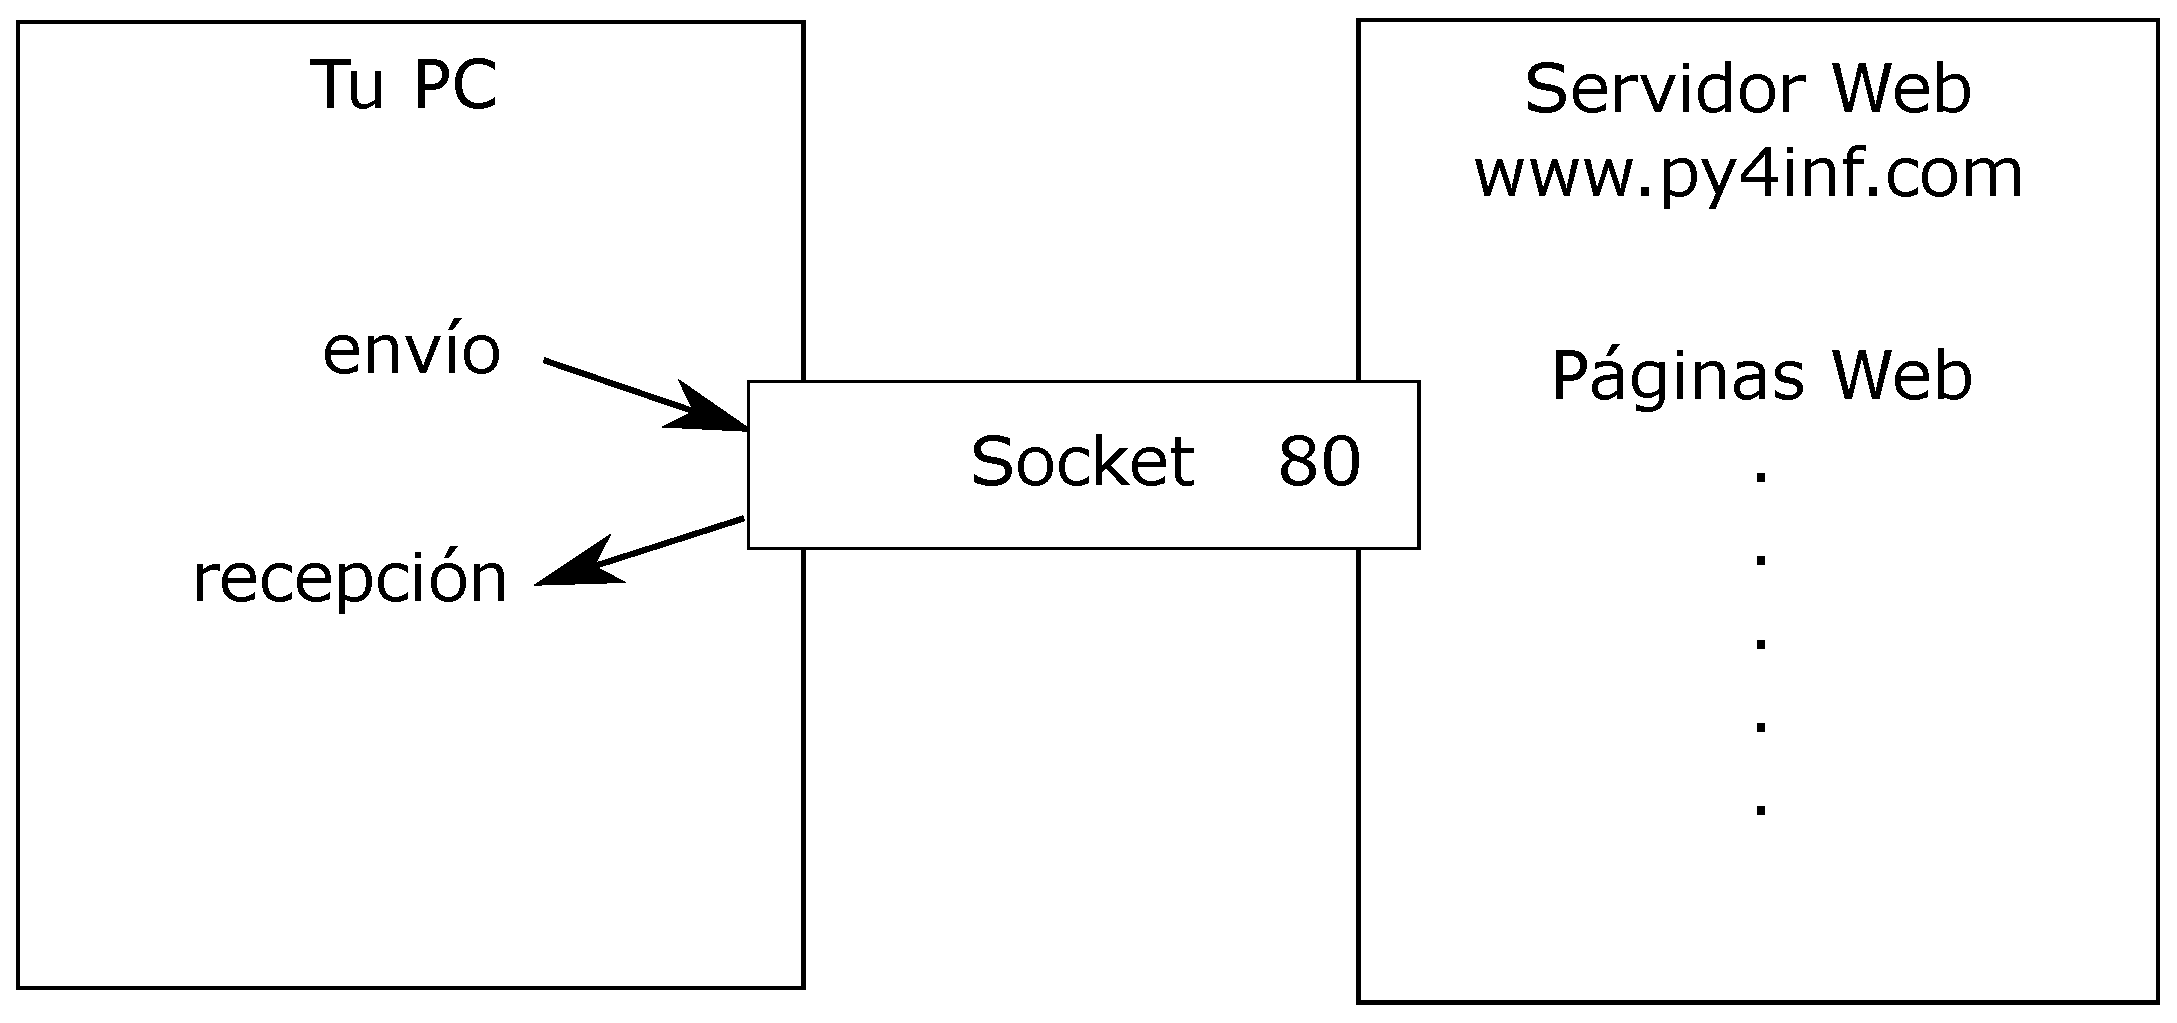
\includegraphics[height=1.50in]{figs2/socket.eps}}
\afterfig

Una vez enviada esa línea en blanco, escribimos un bucle que recibe los datos
desde el socket en bloques de 512 caracteres y los imprime en pantalla
hasta que no quedan más datos por leer (es decir, hasta que recv() devuelve
una cadena vacía).

El programa produce la salida siguiente:

\beforeverb
\begin{verbatim}
HTTP/1.1 200 OK
Date: Sun, 14 Mar 2010 23:52:41 GMT
Server: Apache
Last-Modified: Tue, 29 Dec 2009 01:31:22 GMT
ETag: "143c1b33-a7-4b395bea"
Accept-Ranges: bytes
Content-Length: 167
Connection: close
Content-Type: text/plain

But soft what light through yonder window breaks
It is the east and Juliet is the sun
Arise fair sun and kill the envious moon
Who is already sick and pale with grief
\end{verbatim}
\afterverb
%
La salida comienza con las cabecera que el servidor web envía
para describir el documento.
Por ejemplo, la cabecera {\tt Content-Type} indica que
el documento es del tipo texto plano ({\tt text/plain}).

Después de que el servidor nos envía la cabecera, añade una línea en blanco
para indicar el final de la misma, y a continuación envía los datos
reales del fichero {\tt romeo.txt}.

Este ejemplo nos muestra cómo crear una conexión de red de bajo nivel
con sockets. Los sockets pueden ser usados para comunicarse con un servidor
web, con un servidor de correo o con muchos otros tipos de servidores.
Todo lo que se necesita es localizar el documento que describe
el protocolo correspondiente y escribir el código para enviar y recibir los datos
de acuerdo a ese protocolo.

Sin embargo, como el protocolo que se usa con más frecuencia es
el protocolo web HTTP, Python posee una librería
especial específicamente diseñada para trabajar con ese protocolo
y recibir documentos y datos a través de la web.

\section{Recepción de una imagen mediante HTTP}

\index{imagen!jpg}
\index{jpg}
En el ejemplo anterior, hemos recibido un archivo de texto plano
que tenía saltos de línea en su interior, y lo único que hemos hecho
desde el programa ha sido ir copiando los datos en la pantalla. Podemos usar un programa
similar para recibir una imagen a través de HTTP. En lugar
de copiar los datos a la pantalla según va funcionando el programa,
acumularemos esos datos en una cadena, recortaremos las cabeceras,
y luego guardaremos los datos de la imagen en un archivo, como se muestra a continuación:

\beforeverb
\begin{verbatim}
import socket
import time

misock = socket.socket(socket.AF_INET, socket.SOCK_STREAM)
misock.connect(('www.py4inf.com', 80))
misock.send('GET http://www.py4inf.com/cover.jpg HTTP/1.0\n\n')


contador = 0
imagen = "";
while True:
    datos = misock.recv(5120)
    if ( len(datos) < 1 ) : break
    # time.sleep(0.25)
    contador = contador + len(datos)
    print len(datos),contador
    imagen = imagen + datos

misock.close()

# Búsqueda del final de la cabecera (2 CRLF)
pos = imagen.find("\r\n\r\n");
print 'Longitud de cabecera',pos
print imagen[:pos]

# Saltar detrás de la cabecera y guardar los datos de la imagen
imagen = imagen[pos+4:]
manf = open("cosa.jpg","wb")
manf.write(imagen);
manf.close()
\end{verbatim}
\afterverb
%
Cuando el programa se ejecuta, produce la salida siguiente:

\beforeverb
\begin{verbatim}
$ python urljpeg.py 
2920 2920
1460 4380
1460 5840
1460 7300
...
1460 62780
1460 64240
2920 67160
1460 68620
1681 70301
Longitud de cabecera 240
HTTP/1.1 200 OK
Date: Sat, 02 Nov 2013 02:15:07 GMT
Server: Apache
Last-Modified: Sat, 02 Nov 2013 02:01:26 GMT
ETag: "19c141-111a9-4ea280f8354b8"
Accept-Ranges: bytes
Content-Length: 70057
Connection: close
Content-Type: image/jpeg
\end{verbatim}
\afterverb
%
Puedes observar que, para esta url, la
cabecera {\tt Content-Type} indica que el
cuerpo del documento es una imagen ({\tt image/jpeg}).
Una vez que el programa se completa, se pueden ver los datos de la imagen abriendo
el archivo {\tt cosa.jpg} con un visor de imágenes.

Al ejecutar el programa, se puede ver que no se obtienen 5120 caracteres
cada vez que que se llama al método {\tt recv()}.
Se obtienen tantos caracteres como hayan sido transferidos por el servidor web hacia nosotros
a través de la red en el momento de la llamada a {\tt recv()}.
En este ejemplo, se obtienen 1460 ó 2920 caracteres cada vez que
se solicita un máximo de 5120 caracteres de datos.

Los resultados obtenidos pueden ser diferentes dependiendo de la velocidad de tu red. Además
fíjate en que en la última llamada a {\tt recv()} se obtienen 1681 bytes, que es el final
de la cadena, y en la siguiente llamada a {\tt recv()} se obtiene una cadena de
longitud cero que nos indica que el servidor ya ha llamado a {\tt close()} en su lado
del socket y por tanto no quedan más datos pendientes.

\index{time}
\index{time.sleep}
Podemos retardar las llamadas sucesivas a {\tt recv()} descomentando la llamada
a {\tt time.sleep()}. Así, esperamos un cuarto de segundo después de cada llamada,
de modo que el servidor puede ``adelantarse'' a nosotros y enviarnos más datos
antes de que llamemos de nuevo a {\tt recv()}. Con el retraso, esta vez el programa
se ejecuta así:
\beforeverb
\begin{verbatim}
$ python urljpeg.py 
1460 1460
5120 6580
5120 11700
...
5120 62900
5120 68020
2281 70301
Longitud de cabecera 240
HTTP/1.1 200 OK
Date: Sat, 02 Nov 2013 02:22:04 GMT
Server: Apache
Last-Modified: Sat, 02 Nov 2013 02:01:26 GMT
ETag: "19c141-111a9-4ea280f8354b8"
Accept-Ranges: bytes
Content-Length: 70057
Connection: close
Content-Type: image/jpeg
\end{verbatim}
\afterverb
%
Ahora todas las llamadas a {\tt recv()}, excepto la primera y la última,
nos dan 5120 caracteres cada vez que solicitamos más datos.

Existe un buffer entre el servidor que hace las peticiones {\tt send()}
y nuestra aplicación que hace las peticiones {\tt recv()}. Cuando ejecutamos
el programa con el retraso activado, en algún momento el servidor podría
llenar el buffer del socket y verse forzado a detenerse hasta que
nuestro programa empiece a vaciar ese buffer. La detención de la aplicación
que envía los datos o de la que los recibe se llama
``control de flujo''.
\index{control de flujo}

\section{Recepción de páginas web con {\tt urllib}}

\index{urllib!imagen}
A pesar de que es posible enviar y recibir datos manualmente a través de HTTP
usando la librería socket, existe en Python un modo mucho más sencillo de
realizar esta tarea cotidiana,
usando la librería {\tt urllib}.

Al usar {\tt urllib},
es posible tratar una página web de forma mucho más parecida a un fichero. Se puede
indicar simplemente qué página web se desea recuperar y
{\tt urllib} se encargará de gestionar todo lo referente al protocolo HTTP y
los detalles de la cabecera.

El código equivalente para leer el fichero {\tt romeo.txt}
desde la web usando {\tt urllib} es el siguiente:

\beforeverb
\begin{verbatim}
import urllib

manf = urllib.urlopen('http://www.py4inf.com/code/romeo.txt')
for linea in manf:
   print linea.strip()
\end{verbatim}
\afterverb
%
Una vez que la página web ha sido abierta con
{\tt urllib.urlopen}, se puede tratar como
un archivo y leer a través de ella usando un
bucle {\tt for}.

Cuando el programa se ejecuta, en su salida
sólo vemos el contenido del fichero. Las cabeceras
siguen enviándose, pero el código de {\tt urllib}
se queda con ellas y sólo nos devuelve
los datos.

\beforeverb
\begin{verbatim}
But soft what light through yonder window breaks
It is the east and Juliet is the sun
Arise fair sun and kill the envious moon
Who is already sick and pale with grief
\end{verbatim}
\afterverb
%

Como ejemplo, podemos escribir un
programa para recuperar los datos de
{\tt romeo.txt} y calcular la frecuencia
de cada palabra del fichero, como se muestra a continuación:

\beforeverb
\begin{verbatim}
import urllib

contadores = dict()
manf = urllib.urlopen('http://www.py4inf.com/code/romeo.txt')
for linea in manf:
    palabras = linea.split()
    for palabra in palabras:
        contadores[palabra] = contadores.get(palabra,0) + 1   
print contadores
\end{verbatim}
\afterverb
%
Vemos de nuevo que una vez abierta la página web
se puede leer como si fuera un fichero local.

\section{Análisis de HTML y rascado de la web}
\index{web!scraping}
\index{web!rascado}
\index{HTML!análisis de}

Uno de los usos más habituales de las capacidades de {\tt urllib} en Python
es {\bf rascar} la web. El ``web scraping'' o rascado de la web consiste en escribir un programa
que finge ser un navegador web y recupera páginas, examinando
luego los datos de esas páginas para encontrar ciertos patrones.

Por ejemplo, un motor de búsqueda como Google buscará en el código
de una página web, extraerá los enlaces a otras páginas y recuperará
esas páginas, extrayendo los enlaces que haya en ellas y así sucesivamente. Usando esta técnica,
las  {\bf arañas} de Google se mueven por casi todas las páginas de
la web.

Google utiliza también la frecuencia con que las páginas que encuentra enlazan
hacia una página concreta para calcular la ``importancia'' de
esa página, y la posición en la que debe aparecer dentro de sus resultados de búsqueda.

\section{Análisis de HTML mediante expresiones regulares}

Un modo sencillo de analizar HTML consiste en usar expresiones regulares para
hacer búsquedas repetidas que extraigan subcadenas que coincidan con un patrón concreto.

Aquí tenemos una página web sencilla:

\beforeverb
\begin{verbatim}
<h1>La Primera Página</h1>
<p>
Si te apetece, puedes visitar la
<a href="http://www.dr-chuck.com/page2.htm">
Seguna Página</a>.
</p>
\end{verbatim}
\afterverb
%
Podemos construir una expresión regular bien formada que busque
y extraiga los valores de los enlaces del texto anterior, de éste modo:

\beforeverb
\begin{verbatim}
href="http://.+?"
\end{verbatim}
\afterverb
%
Nuestra expresión regular busca cadenas que comiencen por
``href="http://'', seguido de uno o más caracteres
(``.+?''), seguidos por otra comilla doble. El signo de interrogación
añadido a ``.+?'' indica que la coincidencia debe ser hecha
en modo ``no-codicioso'', en vez de en modo ``codicioso''.
Una búsqueda no-codiciosa intenta encontrar la cadena coincidente
{\em más pequeña} posible, mientras que una búsqueda codiciosa intentaría
localizar la cadena coincidente {\em más grande}.
\index{codicioso}
\index{no codicioso}

Añadimos paréntesis a nuestra expresión regular para indicar
qué parte de la cadena localizada queremos extraer, y
obtenemos el siguiente programa:
\index{regex!paréntesis}
\index{paréntesis!expresiones regulares}

\beforeverb
\begin{verbatim}
import urllib
import re

url = raw_input('Introduce - ')
html = urllib.urlopen(url).read()
enlaces = re.findall('href="(http://.*?)"', html)
for enlace in enlaces:
    print enlace
\end{verbatim}
\afterverb
%
El método {\tt findall} de las expresiones regulares nos proporciona una lista de todas
las cadenas que coinciden con nuestra expresión regular, devolviendo sólo
el texto del enlace situado dentro de las comillas dobles.

Cuando ejecutamos el programa, obtenemos la siguiente salida:

\beforeverb
\begin{verbatim}
python urlregex.py 
Introduce - http://www.dr-chuck.com/page1.htm
http://www.dr-chuck.com/page2.htm

python urlregex.py 
Introduce - http://www.py4inf.com/book.htm
http://www.greenteapress.com/thinkpython/thinkpython.html
http://allendowney.com/
http://www.py4inf.com/code
http://www.lib.umich.edu/espresso-book-machine
http://www.py4inf.com/py4inf-slides.zip
\end{verbatim}
\afterverb
%
Las expresiones regulares funcionan muy bien cuando el HTML está bien formado
y es predecible. Pero dado que ahí fuera hay muchas páginas con HTML ``defectuoso'',
una solución usando solamente expresiones regulares puede o bien
perder parte de los enlaces correctos, o bien terminar obteniendo datos erróneos.

Esto se puede resolver usando una librería de análisis de HTML robusta.

\section{Análisis de HTML mediante BeautifulSoup}
\index{BeautifulSoup}

Hay un buen número de librerías en Python que pueden ayudarte a analizar
HTML y a extraer datos de las páginas. Cada una de las librerías
tiene sus puntos fuertes y flacos, de modo que puedes elegir una
basada en tus necesidades.

Por ejemplo, vamos a analizar simplemente una entrada HTML cualquiera
y a extraer enlaces usando la librería {\bf BeautifulSoup}.
El código de BeautifulSoup se puede descargar e instalar
desde:

\url{http://www.crummy.com/software/}

Se puede descargar e ``instalar'' BeautifulSoup, o
simplemente colocar el archivo {\tt BeautifulSoup.py} en la
misma carpeta que nuestra aplicación.

A pesar de que el HTML se parece al XML\footnote{El formato XML será descrito
en el próximo capítulo.} y que algunas páginas están cuidadosamente
construidas para ser XML, la mayoría del HTML generalmente está
incompleto, de tal modo que provoca que un analizador de XML rechace la página completa de HTML
por estar formada inadecuadamente. BeautifulSoup tolera el HTML
aunque esté muy defectuoso, y aún así permite extraer los datos que se necesiten.

Vamos a usar {\tt urllib} para leer la página y luego usaremos
{\tt BeautifulSoup} para extraer los atributos {\tt href} de las
etiquetas de anclaje ({\tt a}).
\index{BeautifulSoup}
\index{HTML}
\index{análisis!HTML}

\beforeverb
\begin{verbatim}
import urllib
from BeautifulSoup import *

url = raw_input('Introduce - ')
html = urllib.urlopen(url).read()
sopa = BeautifulSoup(html)

# Recupera todas las etiquetas de anclaje
etiquetas = sopa('a')
for etiqueta in etiquetas:
   print etiqueta.get('href', None)
\end{verbatim}
\afterverb
%
El programa solicita una dirección web, luego abre la página
web, lee los datos y se los pasa al analizador BeautifulSoup,
que recupera todas las etiquetas de anclaje e imprime en pantalla
el atributo {\tt href} de cada una de ellas.

Cuando el programa se ejecuta, muestra lo siguiente:

\beforeverb
\begin{verbatim}
python urllinks.py 
Introduce - http://www.dr-chuck.com/page1.htm
http://www.dr-chuck.com/page2.htm

python urllinks.py 
Introduce - http://www.py4inf.com/book.htm
http://www.greenteapress.com/thinkpython/thinkpython.html
http://allendowney.com/
http://www.si502.com/
http://www.lib.umich.edu/espresso-book-machine
http://www.py4inf.com/code
http://www.pythonlearn.com/
\end{verbatim}
\afterverb
%
Se puede utilizar BeautifulSoup para extraer varias partes de cada
etiqueta de este modo:

\beforeverb
\begin{verbatim}
import urllib
from BeautifulSoup import *

url = raw_input('Introduce - ')
html = urllib.urlopen(url).read()
sopa = BeautifulSoup(html)

# Recupera todas las etiquetas de anclaje
etiquetas = sopa('a')
for etiqueta in etiquetas:
   # Busca las partes de una etiqueta
   print 'ETIQUETA:',etiqueta
   print 'URL:',etiqueta.get('href', None)
   print 'Contenido:',etiqueta.contents[0]
   print 'Atributos:',etiqueta.attrs
\end{verbatim}
\afterverb
%
Esto produce la siguiente salida:

\beforeverb
\begin{verbatim}
python urllink2.py 
Introduce - http://www.dr-chuck.com/page1.htm
ETIQUETA: <a href="http://www.dr-chuck.com/page2.htm">
Second Page</a>
URL: http://www.dr-chuck.com/page2.htm
Contenido: [u'\nSecond Page']
Atributos: [(u'href', u'http://www.dr-chuck.com/page2.htm')]
\end{verbatim}
\afterverb
%
Estos ejemplos tan sólo insinúan la potencia de BeautifulSoup
en el análisis del HTML. Lee la documentación y
los ejemplos que están en
\url{http://www.crummy.com/software/BeautifulSoup/} para obtener más detalles.

\section{Lectura de archivos binarios mediante urllib}

A veces se quiere recuperar un fichero que no es de texto (o binario), como
un archivo de imagen o video. Normalmente no resulta útil imprimir los datos de
estos ficheros, pero se puede hacer una copia de una URL en un archivo
local de nuestro disco duro con facilidad, usando {\tt urllib}.
\index{fichero!binario}

La pauta a seguir consiste en abrir la URL y usar {\tt read} para descargar el contenido
completo del documento en una variable de tipo cadena ({\tt img}), y luego escribir la
información a un archivo local, como se muestra a continuación:

\beforeverb
\begin{verbatim}
img = urllib.urlopen('http://www.py4inf.com/cover.jpg').read()
manf = open('portada.jpg', 'w')
manf.write(img)
manf.close()
\end{verbatim}
\afterverb
%
Este programa lee todos los datos de una sola vez a través de la red y los
almacena en la variable {\tt img} en la memoria principal de tu ordenador,
luego abre el fichero {\tt portada.jpg} y escribe los datos en el
disco. Esto funcionará sólo si el tamaño del fichero es menor que el tamaño
de la memoria de tu ordenador.

Sin embargo, si se trata de un fichero enorme de audio o video, el programa puede fallar
o al menos funcionar extremadamente lento cuando el ordenador se quede sin memoria.
Para evitar agotar la memoria, vamos a recuperar los datos en bloques
(o buffers), y luego escribiremos cada bloque en el disco antes de recuperar
el siguiente. De este modo el programa podrá leer archivos de cualquier tamaño sin
usar toda la memoria del equipo.

\beforeverb
\begin{verbatim}
import urllib

img = urllib.urlopen('http://www.py4inf.com/cover.jpg')
manf = open('portada.jpg', 'w')
tamano = 0
while True:
    info = img.read(100000)
    if len(info) < 1 : break
    tamano = tamano + len(info)
    manf.write(info)

print tamano,'caracteres copiados.'
manf.close()
\end{verbatim}
\afterverb
%
En este ejemplo, leemos solamente 100.000 caracteres cada vez y luego
escribimos esos caracteres en el archivo {\tt cover.jpg}
antes de recuperar los 100.000 caracteres siguientes de datos desde
la web.

El programa funciona de este modo:

\beforeverb
\begin{verbatim}
python curl2.py 
568248 caracteres copiados.
\end{verbatim}
\afterverb
%

Si tienes un ordenador Unix o Macintosh, probablemente tendrás un comando
incorporado en tu sistema operativo que puede realizar esa misma operación
de este modo:
\index{curl}

\beforeverb
\begin{verbatim}
curl -O http://www.py4inf.com/cover.jpg
\end{verbatim}
\afterverb
%
El comando {\tt curl} es la abreviatura de ``copy URL'' y por eso estos dos
ejemplos se han llamado astutamente {\tt curl1.py} y {\tt curl2.py} en
\url{www.py4inf.com/code}, ya que implementan una funcionalidad similar
a la del comando {\tt curl}. Existe también un programa de ejemplo {\tt curl3.py}
que realiza la misma tarea de forma un poco más eficiente, en caso de
que quieras usar de verdad este patrón en algún programa que estés escribiendo.

\section{Glosario}

\begin{description}

\item[BeautifulSoup:] Una librería Python para analizar documentos HTML
y extaer datos de ellos
que compensa la mayoría de las imperfecciones que los navegadores HTML
normalmente ignoran.
Puedes descargar el código de BeautifulSoup
desde
\url{www.crummy.com}.
\index{BeautifulSoup}

\item[puerto:] Un número que generalmente indica con qué aplicación
estás contactando cuando realizas una conexión con un socket en un servidor.
Por ejemplo, el tráfico web normalmente usa el puerto 80, mientras que el tráfico
del correo electrónico usa el puerto 25.
\index{puerto}

\item[rastrear:] La acción de un motor de búsqueda web de recuperar una página
y luego todas las páginas enlazadas por ella, continuando así sucesivamente hasta que
tiene casi todas las páginas de Internet, que
usan para construir su índice de búsqueda.
\index{spider}
\index{rastrear}

\item[socket:] Una conexión de red entre dos aplicaciones,
en la cual dichas aplicaciones pueden enviar y recibir datos en ambas direcciones.
\index{socket}

\item[scraping (rascado):] Cuando un programa simula ser un navegador web y
recupera una página web, y luego realiza una búsqueda en su contenido.
A menudo los programas siguen los enlaces en una página para encontrar la
siguiente, de modo que pueden atravesar una red de páginas o una red social.
\index{scrape}
\index{rascado}

\end{description}

\section{Ejercicios}

\begin{ex}
Cambia el programa del socket {\tt socket1.py} para que le pida al usuario
la URL, de modo que pueda leer cualquier página web.
Puedes usar {\tt split('/')} para dividir la URL en las partes que la componen,
de modo que puedas extraer el nombre del host para la llamada a {\tt connect} del socket.
Añade comprobación de errores, usando {\tt try} y {\tt except} para gestionar el caso de que
el usuario introduzca una URL mal formada o inexistente.  
\end{ex}

\begin{ex}
Cambia el programa del socket para que cuente el número de caracteres que ha recibido
y se detenga, con un texto en pantalla, después de que se hayan mostrado 3000 caracteres. El programa
debe recuperar el documento completo y contar el número total de caracteres,
mostrando ese total al final del documento.
\end{ex}

\begin{ex}
Usa {\tt urllib} para rehacer el ejercicio anterior de modo que (1) reciba el documento
de una URL, (2) muestre hasta 3000 caracteres, y (3) cuente la cantidad total
de caracteres en el documento. No te preocupes de las cabeceras en este ejercicio,
muestra simplemente los primeros 3000 caracteres del contenido del documento.
\end{ex}

\begin{ex}
Cambia el programa {\tt urllinks.py} para extraer y contar
las etiquetas de párrafo (p) del documento HTML recuperado y
mostrar el total de párrafos como
salida del programa.
No muestres el texto de los párrafos, sólo cuéntalos.
Prueba el programa en varias páginas web pequeñas,
y también en otras más grandes.
\end{ex}

\begin{ex}
(Avanzado) Cambia el programa del socket, de modo que sólo muestre los datos
después de que se haya recibido la cabecera y la línea en blanco. Recuerda que {\tt recv}
va recibiendo caracteres (saltos de línea incluidos), y no líneas.
\end{ex}
% The contents of this file is 
% Copyright (c) 2009-  Charles R. Severance, All Righs Reserved

\chapter{Uso de servicios web}

Una vez que recuperar documentos a través de HTTP y analizarlos usando
programas se convirtió en algo sencillo,
no se tardó demasiado en desarrollar un modelo
consistente en la producción de
documentos específicamente diseñados para ser consumidos por otros
programas (es decir, no únicamente HTML para ser mostrado en un navegador).

Existen dos formatos habituales que se usan para el intercambio de datos a través de la web.
El ``eXtensible Markup Language'' (lenguaje extensible de marcas), o XML, ha sido utilizado
durante mucho tiempo, y es el más adecuado para intercambiar datos del tipo-documento.
Cuando los programas simplemente quieren intercambiar unos con otros diccionarios, listas u otra
información interna, usan ``JavaScript Object Notation'' (Notación de Objetos Javascript), o JSON
(consulta \url{www.json.org}). Nosotros vamos a revisar ambos formatos.

\section{eXtensible Markup Language - XML}

XML tiene un aspecto muy parecido a HTML, pero XML está más estructurado.
Esto es un ejemplo de un documento XML:

\beforeverb
\begin{verbatim}
<persona>
  <nombre>Chuck</nombre>
  <telefono tipo="intl">
     +1 734 303 4456
   </telefono>
   <email oculto="si"/>
</persona>
\end{verbatim}
\afterverb
%
A veces resulta útil pensar en un documento XML como en la estructura de un árbol,
donde hay una etiqueta superior {\tt persona}, y otras etiquetas como {\tt telefono}
que se dibujan como \emph{hijas} de sus nodos padres.

\beforefig
\centerline{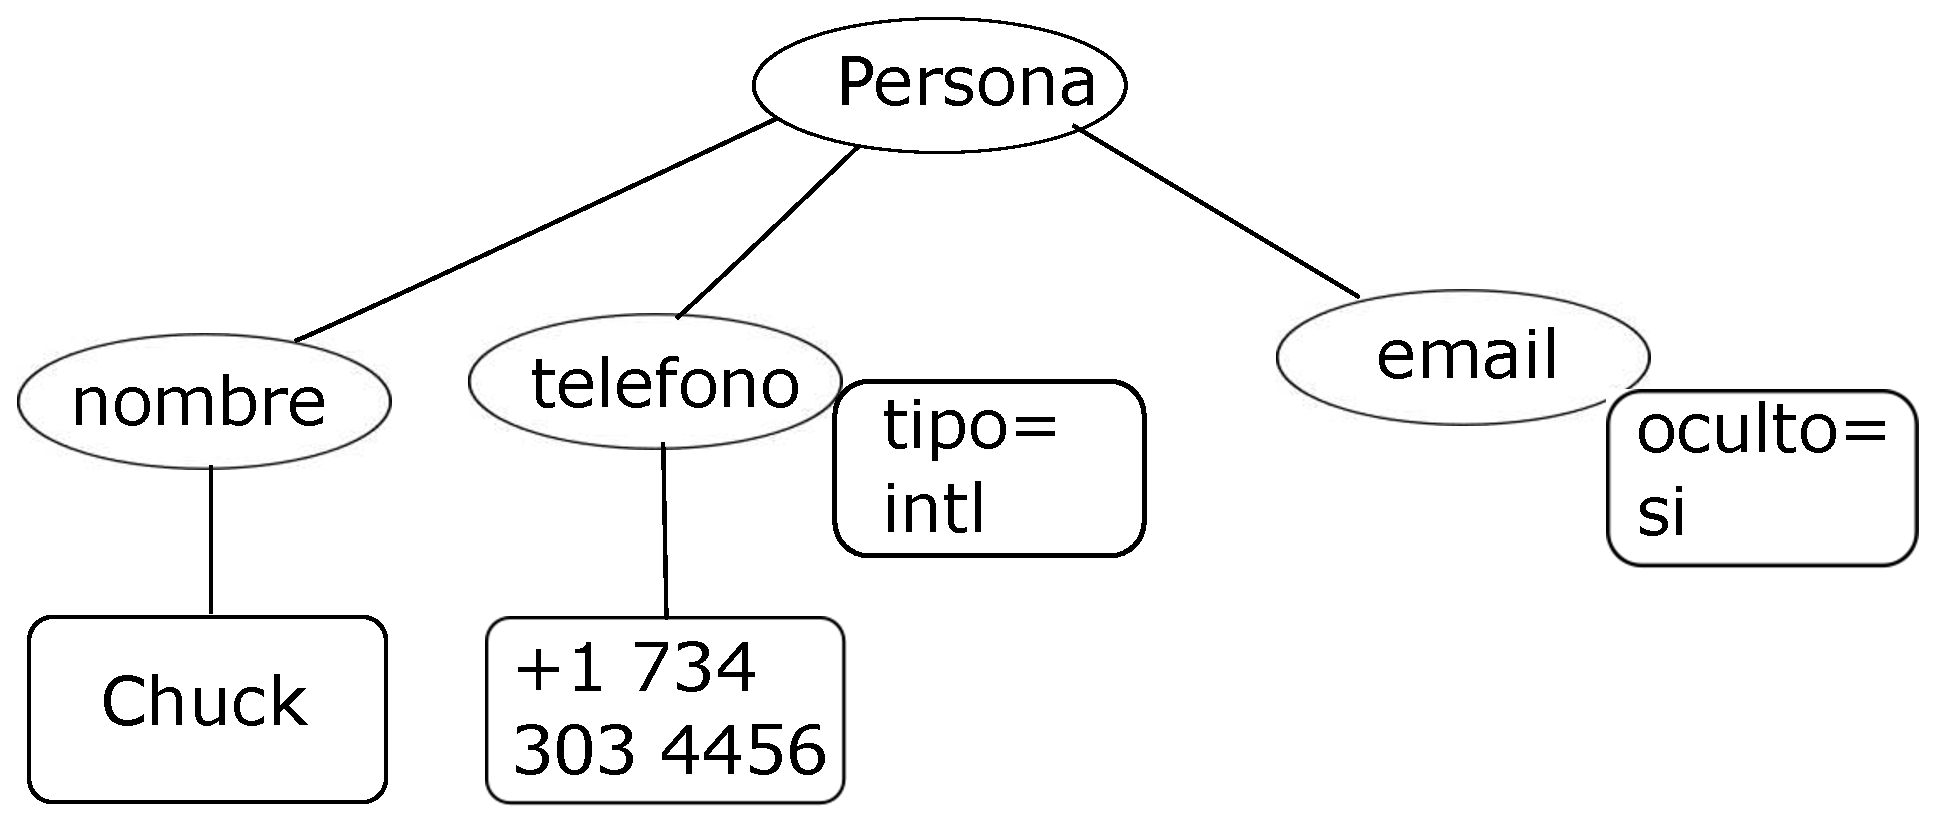
\includegraphics[height=1.50in]{figs2/xml-tree.eps}}
\afterfig

\section{Análisis de XML}

\index{ElementTree}
\index{ElementTree!fromstring}
\index{ElementTree!find}
He aquí una aplicación sencilla que analiza el XML anterior
y extrae algunos elementos de él:

\beforeverb
\begin{verbatim}
import xml.etree.ElementTree as ET

datos = '''
<persona>
  <nombre>Chuck</nombre>
  <telefono tipo="intl">
     +1 734 303 4456
   </telefono>
   <email oculto="si"/>
</persona>'''

arbol = ET.fromstring(datos)
print 'Nombre:',arbol.find('nombre').text
print 'Attr:',arbol.find('email').get('oculto')
\end{verbatim}
\afterverb
%
La llamada a {\tt fromstring} convierte la representación de cadena
del XML en un ``árbol'' de nodos XML. Una vez tenemos el XML
como un árbol, disponemos de una serie de métodos que podemos llamar para
extraer porciones de datos de ese XML.

La función {\tt find} busca a través del árbol XML
y recupera un {\bf nodo} que coincide con la etiqueta especificada.
Cada nodo tiene cierto texto, ciertos atributos (como en este caso ``oculto''), y
ciertos nodos ``hijos''. Cada nodo puede ser el origen de otro árbol de nodos.

\beforeverb
\begin{verbatim}
Nombre: Chuck
Attr: si
\end{verbatim}
\afterverb
%
El usar un analizador de XML como {\tt ElementTree} tiene la ventaja
de que, a pesar de que el XML de este ejemplo es bastante sencillo, resulta
que hay un montón de reglas respecto a la validez del XML, y el uso de
{\tt ElementTree} nos permite extraer datos del XML sin
preocuparnos acerca de esas reglas de sintaxis.

\section{Desplazamiento a través de los nodos}

\index{ElementTree!findall}
\index{ElementTree!get}
A menudo el XML tiene múltiples nodos y tenemos que escribir un bucle
para procesarlos todos. En el programa siguiente,
usamos un bucle para recorrer todos los nodos {\tt usuario}:

\beforeverb
\begin{verbatim}
import xml.etree.ElementTree as ET

entrada = '''
<cosas>
    <usuarios>
        <usuario x="2">
            <id>001</id>
            <nombre>Chuck</nombre>
        </usuario>
        <usuario x="7">
            <id>009</id>
            <nombre>Brent</nombre>
        </usuario>
    </usuarios>
</cosas>'''

cosas = ET.fromstring(entrada)
lst = cosas.findall('usuarios/usuario')
print 'Cantidad de usuarios:', len(lst)

for elemento in lst:
    print 'Nombre', elemento.find('nombre').text
    print 'Id', elemento.find('id').text
    print 'Atributo', elemento.get('x')
\end{verbatim}
\afterverb
%
El método {\tt findall} devuelve a Python una lista de subárboles que
representan las estructuras {\tt usuario} del árbol XML. A continuación podemos
escribir un bucle {\tt for} que busque en cada uno de los nodos usuario,
e imprima el texto de los elementos {\tt nombre} e {\tt id}, además del
atributo {\tt x} de cada nodo {\tt usuario}.

\beforeverb
\begin{verbatim}
Cantidad de usuarios: 2
Nombre Chuck
Id 001
Atributo 2
Nombre Brent
Id 009
Atributo 7
\end{verbatim}
\afterverb
%

\section{JavaScript Object Notation - JSON}
\index{JSON}
\index{JavaScript Object Notation}

El formato JSON se inspiró en el formato de objetos y arrays que se usa en el lenguaje
JavaScript. Pero como Python se inventó antes que JavaScript, la sintaxis usada en Python
para los diccionarios y listas influyeron la sintaxis de JSON. De modo que el formato
del JSON es casi idéntico a la combinación de listas y diccionarios de Python.

He aquí una codificación JSON que es más o menos equivalente al XML del ejemplo anterior:

\beforeverb
\begin{verbatim}
{
  "nombre" : "Chuck",
  "telefono" : {
    "tipo" : "intl",
    "numero" : "+1 734 303 4456"
   },
   "email" : {
     "oculto" : "si"
   }
}
\end{verbatim}
\afterverb
%
Si te fijas, encontrarás ciertas diferencias. La primera, en XML se pueden añadir atributos como
``intl'' a la etiqueta ``telefono''. En JSON, simplemente tenemos parejas clave-valor.
Además, la etiqueta ``persona'' de XML ha desaparecido, reemplazada por un conjunto
de llaves exteriores.

En general, las estructuras JSON son más simples que las de XML, debido a que JSON tiene
menos capacidades. Pero JSON tiene la ventaja de que mapea {\em directamente} hacia una
combinación de diccionarios y listas. Y dado que casi todos los lenguajes de programación
tienen algo equivalente a los diccionarios y listas de Python, JSON es un formato
muy intuitivo para que dos programas que vayan a cooperar intercambien datos.

JSON se está convirtiendo rápidamente en el formato elegido para casi todos los intercambios
de datos entre aplicaciones, debido a su relativa simplicidad comparado con XML.

\section{Análisis de JSON}

El JSON se construye anidando diccionarios (objetos) y listas según se necesite.
En este ejemplo, vamos a representar una lista de usuarios en la cual cada usuario es un
conjunto de parejas clave-valor (es decir, un diccionario). De modo que tendremos una lista
de diccionarios.

En el programa siguiente, usaremos la librería integrada {\bf json} para analizar
el JSON y leer los datos. Compáralo cuidadosamente con los datos y código XML
equivalentes que usamos antes. El JSON tiene menos detalles, de modo que podemos saber de
antemano que vamos a obtener una lista y que la lista es de usuarios y además que cada usuario es un
conjunto de parejas clave-valor. El JSON es más conciso (una ventaja), pero también es
menos auto-descriptivo (una desventaja).

\beforeverb
\begin{verbatim}
import json

entrada = '''
[
  { "id" : "001",
    "x" : "2",
    "nombre" : "Chuck"
  } ,
  { "id" : "009",
    "x" : "7",
    "nombre" : "Brent"
  } 
]'''

info = json.loads(entrada)
print 'Cantidad de usuarios:', len(info)

for elemento in info:
    print 'Nombre', elemento['nombre']
    print 'Id', elemento['id']
    print 'Atributo', elemento['x']
\end{verbatim}
\afterverb
%
Si comparas el código que extrae los datos del JSON analizado y el del XML,
verás que lo que obtenemos de {\bf json.loads()} es una lista de Python
que recorreremos con un bucle {\tt for}, y cada elemento dentro de esa lista
es un diccionario de Python. Una vez analizado el JSON, podemos usar el operador
índice de Python para extraer los distintos fragmentos de datos de cada usuario. No
tenemos que usar la librería JSON para rebuscar a través del JSON analizado, ya que los
datos devueltos son sencillamente estructuras nativas de Python.

La salida de este programa es exactamente la misma que la de la versión XML anterior.

\beforeverb
\begin{verbatim}
Cantidad de usuarios: 2
Nombre Chuck
Id 001
Atributo 2
Nombre Brent
Id 009
Atributo 7
\end{verbatim}
\afterverb
%
En general, hay una tendencia en la industria a apartarse del XML y pasar al JSON para
los servicios web. Como el JSON es más sencillo, y se mapea de forma más directa hacia
estructuras de datos nativas que ya tenemos en los lenguajes de programación, el código de
análisis y extracción de datos normalmente es más sencillo y directo usando JSON.
Sin embargo, XML es más auto-descriptivo, y por eso hay ciertas
aplicaciones en las cuales XML mantiene su ventaja. Por ejemplo, la mayoría de los
procesadores de texto almacenan sus documentos internamente usando XML en vez de JSON.

\section{Interfaces de programación de aplicaciones}

Ahora ya tenemos la capacidad de intercambiar datos entre aplicaciones usando el Protocolo
de Transporte de Hipertexto (HTTP), y un modo de representar estructuras de datos complejas
para poder enviar y recibir los datos entre esas aplicaciones, a través del eXtensible 
Markup Language (XML) o del JavaScript Object Notation (JSON).

El paso siguiente consiste en empezar a definir y documentar ``contratos'' entre
aplicaciones usando estas técnicas. El nombre habitual para estos
contratos entre aplicaciones es {\bf Interfaces de Programación
de Aplicaciones} ({\tt Application Program Interfaces}), o APIs. Cuando se utiliza una API, normalmente un programa
crea un conjunto de {\bf servicios} disponibles para que los usen otras aplicaciones
y publica las APIs (es decir, las ``reglas'') que deben ser seguidas para
acceder a los servicios proporcionados por el programa.

Cuando comenzamos a construir programas con funcionalidades que incluyen
el acceso a servicios proporcionados por otros,
se utiliza un planteamiento llamado {\bf Arquitectura Orientada a Servicios}
({\tt Service-Oriented Architecture}), o SOA.
Un planteamiento SOA es aquel en el cual nuestra aplicación principal usa los servicios
de otras aplicaciones. Un planteamiento no-SOA es aquel en el cual tenemos
una única aplicación independiente que contiene ella misma todo el código
necesario para su implementación.

Podemos encontrar multitud de ejemplos de SOAs cuando utilizamos servicios de la web. Podemos ir a un
único sitio web y reservar viajes en avión, hoteles y automóviles, todo ello desde el
mismo sitio. Los datos de los hoteles no están almacenados en los equipos de la
compañía aérea. En vez de eso, los equipos de la aerolínea contactan con los servicios
de las máquinas de los hoteles y recuperan los datos de los alojamientos que presentan al
usuario. Cuando el usuario acepta realizar una reserva de un hotel usando el sitio web
de una aerolínea, ésta utiliza otro servicio web en los sistemas de los hoteles para realizar
la reserva real. Y cuando llega el momento de cargar en tu tarjeta de crédito el importe de la
transacción completa, hay todavía otros equipos diferentes involucrados en el proceso.

\beforefig
\centerline{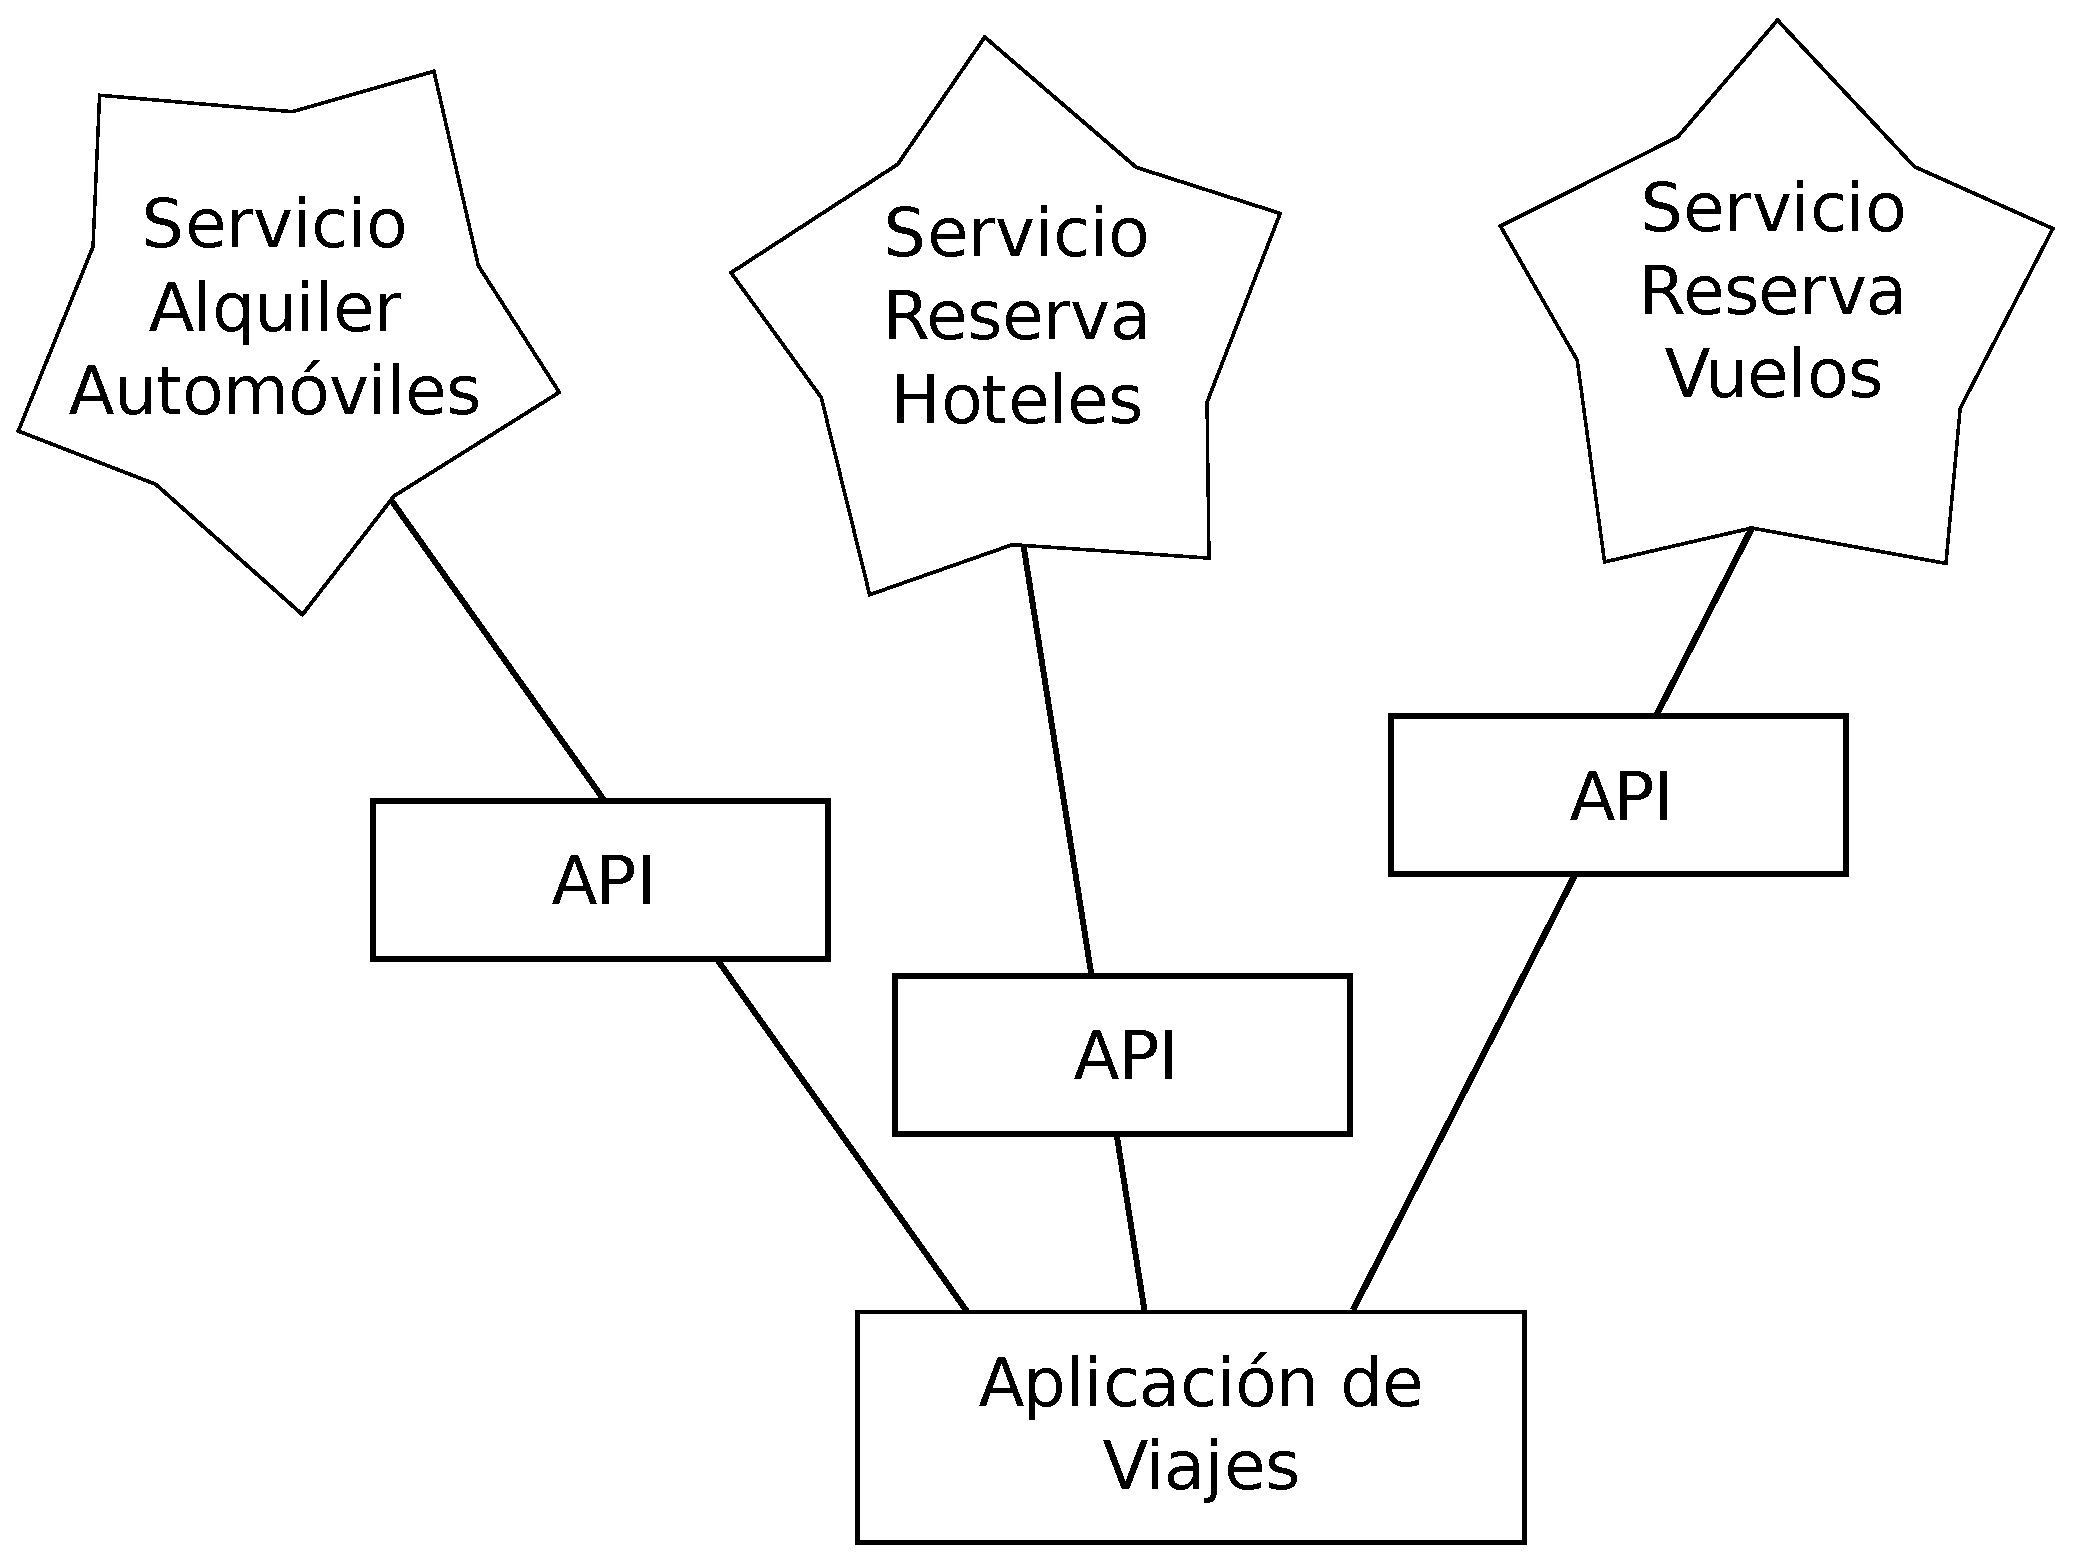
\includegraphics[height=2.50in]{figs2/soa.eps}}
\afterfig

Una Arquitectura Orientada a Servicios tiene muchas ventajas, que incluyen: (1)
siempre se mantiene una única copia de los datos (lo cual resulta particularmente
importante en ciertas cosas como las reservas hoteleras, que no se pueden duplicar)
y (2) los propietarios de los datos pueden imponer las reglas acerca del uso de esos datos.
Con estas ventajas, un sistema SOA debe ser diseñado con mucho cuidado para
tener buen rendimiento y satisfacer las necesidades de los usuarios.

Cuando una aplicación ofrece un conjunto de servicios en su API disponibles a través de la
web, éstos reciben el nombre de {\bf servicios web}.

\section{Servicio web de geocodificación de Google}
\index{Google}
\index{geocodificación}
\index{servicio web}

Google tiene un servicio web excelente que nos permite hacer uso de su
enorme base de datos de información geográfica. Podemos enviar una cadena de búsqueda
geográfica, como ``Ann Arbor, MI'' a su API de geocodificación y conseguir que Google
nos devuelva la situación en un mapa de dónde podría estar nuestra cadena de
búsqueda, además de los puntos de referencia en los alrededores.

El servicio de geocodificación es gratuito, pero limitado, de modo que no se puede hacer
un uso intensivo de esta API en una aplicación comercial. Pero si tienes ciertos datos
estadísticos en los cuales un usuario final ha introducido una localización en formato
libre en un cuadro de texto, puedes utilizar esta API para limpiar esos datos de forma
bastante efectiva.

{\em Cuando se usa una API libre, como la API de geocodificación de Google, se debe ser
respetuoso con el uso de los recursos. Si hay demasiada gente que abusa del servicio,
Google puede interrumpir o restringir significativamente su uso gratuito.}
\index{límite de uso}

Puedes leer la documentación online de este servicio, pero es bastante sencillo
y puedes incluso probarlo desde un navegador, simplemente tecleando la siguiente URL
en él:

\url{http://maps.googleapis.com/maps/api/geocode/json?sensor=false &address=Ann+Arbor%2C+MI}

Asegúrate de limpiar la URL y eliminar cualquier espacio de ella antes de pegarla
en el navegador.

La siguiente es una aplicación sencilla que pide al usuario una cadena de búsqueda,
llama a la API de geocodificación de Google y extrae información del JSON que nos devuelve.

\beforeverb
\begin{verbatim}
import urllib
import json

urlservicio = 'http://maps.googleapis.com/maps/api/geocode/json?'

while True:
    direccion = raw_input('Introduzca ubicación: ')
    if len(direccion) < 1 : break

    url = urlservicio + urllib.urlencode({'sensor':'false', 
          'address': direccion})
    print 'Recuperando', url
    uh = urllib.urlopen(url)
    datos = uh.read()
    print 'Recibidos',len(datos),'caracteres'

    try: js = json.loads(str(datos))
    except: js = None
    if 'status' not in js or js['status'] != 'OK':
        print '==== Fallo de Recuperación ===='
        print datos
        continue

    print json.dumps(js, indent=4)

    lat = js["results"][0]["geometry"]["location"]["lat"]
    lng = js["results"][0]["geometry"]["location"]["lng"]
    print 'lat',lat,'lng',lng
    ubicacion = js['results'][0]['formatted_address']
    print ubicacion
\end{verbatim}
\afterverb
%
El programa toma la cadena de búsqueda y construye una URL
codificándola como parámetro dentro de ella, utilizando luego
{\bf urllib} para recuperar el texto de la API de geocodificación de Google.
A diferencia de una página web estática, los datos que obtengamos dependerán de los
parámetros que enviemos y de los datos geográficos almacenados en los servidores de Google.

Una vez recuperados los datos JSON, los analizamos con la librería
{\bf json} y realizamos unas pequeñas comprobaciones para asegurarnos de que hemos recibido
datos válidos. Finalmente, extraemos la información que estábamos buscando.

La salida del programa es la siguiente (parte del JSON recibido
ha sido eliminado):

\beforeverb
\begin{verbatim}
$ python geojson.py
Introduzca ubicación: Ann Arbor, MI
Recuperando http://maps.googleapis.com/maps/api/
  geocode/json?sensor=false&address=Ann+Arbor%2C+MI
Recibidos 1669 caracteres
{
    "status": "OK", 
    "results": [
        {
            "geometry": {
                "location_type": "APPROXIMATE", 
                "location": {
                    "lat": 42.2808256, 
                    "lng": -83.7430378
                }
            }, 
            "address_components": [
                {
                    "long_name": "Ann Arbor", 
                    "types": [
                        "locality", 
                        "political"
                    ], 
                    "short_name": "Ann Arbor"
                } 
            ], 
            "formatted_address": "Ann Arbor, MI, USA", 
            "types": [
                "locality", 
                "political"
            ]
        }
    ]
}
lat 42.2808256 lng -83.7430378
Ann Arbor, MI, USA
Introduce ubicación:
\end{verbatim}
\afterverb
%
Puedes descargar
\url{www.py4inf.com/code/geojson.py} y
\url{www.py4inf.com/code/geoxml.py} para revisar
las variantes JSON y XML de la API de geocodificación de Google.

\section{Seguridad y uso de APIs}
\index{OAuth}
\index{API!clave}

Resulta bastante frecuente que se necesite algún tipo de
``clave API'' para hacer uso de una API comercial. La
idea general es que ellos quieren saber quién está usando
sus servicios y cuánto los utiliza cada usuario.
Tal vez tienen distintos niveles (gratuitos y de pago) de sus servicios,
o una política que limita el número de peticiones
que un único usuario puede realizar durante un determinado
periodo de tiempo.

En ocasiones, una vez que tienes tu clave API, tan sólo debes incluirla
como parte de los datos POST, o tal vez como parámetro
dentro de la URL que usas para llamar a la API.

Otras veces, el vendedor quiere aumentar la seguridad del
origen de las peticiones, de modo que además espera que
envíes mensajes firmados criptográficamente, usando claves
compartidas y secretas. Una tecnología muy habitual que se utiliza
para firmar peticiones en Internet se llama {\bf OAuth}.
Puedes leer más acerca del protocolo OAuth en 
\url{http://www.oauth.net}.

A medida que la API de Twitter ha ido haciéndose más valiosa, Twitter
ha pasado de una API abierta y pública a una API que necesita
el uso de firmas OAuth en cada solicitud. Afortunadamente,
aún hay unas cuantas librerías OAuth útiles y gratuitas,
de modo que te puedes ahorrar el tener que escribir una implementación OAuth
desde cero leyendo las especificaciones. Estas librerías tienen
una complejidad variable y varios niveles distintos en cuanto a variedad de características.
El sitio web OAuth tiene información sobre varias librerías OAuth.

Para el programa de ejemplo siguiente, descargaremos los ficheros
{\bf twurl.py}, {\bf hidden.py}, 
{\bf oauth.py}, 
y
{\bf twitter1.py} desde
\url{www.py4inf.com/code}, y los pondremos todos juntos en una carpeta
de tu equipo.

Para usar estos programas debes tener una cuenta de Twitter,
y autorizar a tu código Python como aplicación permitida,
estableciendo diversos parámetros (key, secret, token y token secret). Luego deberás editar
el archivo {\bf hidden.py} y colocar esas cuatro cadenas en las
variables apropiadas dentro del fichero:

\beforeverb
\begin{verbatim}
    def auth() :
        return { "consumer_key" : "h7L...GNg",
            "consumer_secret" : "dNK...7Q",
            "token_key" : "101...GI",
            "token_secret" : "H0yM...Bo" }
\end{verbatim}
\afterverb
%
Se puede acceder al servicio web de Twitter mediante una URL como ésta:

\url{https://api.twitter.com/1.1/statuses/user_timeline.json}

Pero una vez que se ha añadido toda la información de seguridad, la URL
se parecerá más a esto:

\beforeverb
\begin{verbatim}
https://api.twitter.com/1.1/statuses/user_timeline.json?count=2
&oauth_version=1.0&oauth_token=101...SGI&screen_name=drchuck
&oauth_nonce=09239679&oauth_timestamp=1380395644
&oauth_signature=rLK...BoD&oauth_consumer_key=h7Lu...GNg
&oauth_signature_method=HMAC-SHA1
\end{verbatim}
\afterverb
%
Puedes leer la especificación OAuth si quieres saber más
acerca del significado de los distintos parámetros que
hemos añadido para cumplir con los requerimientos de seguridad de OAuth.

Para los programas que ejecutamos con Twitter, ocultamos toda la
complejidad dentro de los archivos {\bf oauth.py} y {\bf twurl.py}.
Simplemente ajustamos los parámetros secretos en {\bf hidden.py}, luego
enviamos la URL deseada a la función {\bf twurl.augment()}
y el código de la librería añade todos los parámetros
necesarios a la URL por nosotros.

Este programa ({\bf twitter1.py}) recupera la línea de tiempo
de un usuario de Twitter concreto y nos la devuelve en formato
JSON como una cadena. Vamos a imprimir simplemente los primeros 250
caracteres de esa cadena:

\beforeverb
\begin{verbatim}
import urllib
import twurl

TWITTER_URL='https://api.twitter.com/1.1/statuses/user_timeline.json'

while True:
    print ''
    cuenta = raw_input('Introduzca Cuenta de Twitter:')
    if ( len(cuenta) < 1 ) : break
    url = twurl.augment(TWITTER_URL,
        {'screen_name': cuenta, 'count': '2'} )
    print 'Recuperando', url
    conexion = urllib.urlopen(url)
    datos = conexion.read()
    print datos[:250]
    cabeceras = conexion.info().dict
    # print cabeceras
    print 'Restante', cabeceras['x-rate-limit-remaining']
\end{verbatim}
\afterverb
%
Cuando el programa se ejecuta, produce la salida siguiente: 
 
\beforeverb
\begin{verbatim}
Introduzca Cuenta de Twitter:drchuck
Recuperando https://api.twitter.com/1.1/ ...
[{"created_at":"Sat Sep 28 17:30:25 +0000 2013","
id":384007200990982144,"id_str":"384007200990982144",
"text":"RT @fixpert: See how the Dutch handle traffic 
intersections: http:\/\/t.co\/tIiVWtEhj4\n#brilliant",
"source":"web","truncated":false,"in_rep
Restante 178

Introduzca Cuenta de Twitter:fixpert
Recuperando https://api.twitter.com/1.1/ ...
[{"created_at":"Sat Sep 28 18:03:56 +0000 2013",
"id":384015634108919808,"id_str":"384015634108919808",
"text":"3 months after my freak bocce ball accident, 
my wedding ring fits again! :)\n\nhttps:\/\/t.co\/2XmHPx7kgX",
"source":"web","truncated":false,
Restante 177

Introduzca Cuenta de Twitter:
\end{verbatim}
\afterverb
%
Junto con los datos de la línea del tiempo, Twitter también devuelve
metadatos sobre la petición, en las cabeceras de respuesta HTTP.
Una cabecera en particular, {\bf x-rate-limit-remaining}, nos informa
sobre cuántas peticiones podremos hacer antes de que seamos bloqueados
por un corto periodo de tiempo. Puedes ver cómo cada vez que realizamos
una petición a la API nuestros intentos restantes van disminuyendo.

En el ejemplo siguiente, recuperamos los amigos de un usuario en Twitter,
analizamos el JSON devuelto y extraemos parte de la información
sobre esos amigos. Después de analizar el JSON e ``imprimirlo bonito'',
realizamos un volcado completo con un justificado de cuatro caracteres, para permitirnos
poder estudiar minuciosamente los datos en el caso de que queramos extraer más campos.

\beforeverb
\begin{verbatim}
import urllib
import twurl
import json

TWITTER_URL = 'https://api.twitter.com/1.1/friends/list.json'

while True:
    print ''
    cuenta = raw_input('Introduzca Cuenta de Twitter:')
    if ( len(cuenta) < 1 ) : break
    url = twurl.augment(TWITTER_URL,
        {'screen_name': cuenta, 'count': '5'} )
    print 'Recuperando', url
    conexion = urllib.urlopen(url)
    datos = conexion.read()
    cabeceras = conexion.info().dict
    print 'Restantes', cabeceras['x-rate-limit-remaining']
    js = json.loads(datos)
    print json.dumps(js, indent=4)

    for u in js['users'] :
        print u['screen_name']
        s = u['status']['text']
        print '  ',s[:50]
\end{verbatim}
\afterverb
%
Dado que el JSON se transforma en un conjunto de listas y diccionarios de Python,
podemos usar una combinación del operador índice junto con bucles {\tt for} para
movernos a través de las estructuras de datos devueltas con muy poco
código Python.

La salida del programa se parece a la siguiente (parte de los datos
se han acortado para que quepa en la página):

\beforeverb
\begin{verbatim}
Introduzca Cuenta de Twitter:drchuck
Recuperando https://api.twitter.com/1.1/friends ...
Restantes 14
{
    "next_cursor": 1444171224491980205, 
    "users": [
        {
            "id": 662433, 
            "followers_count": 28725, 
            "status": {
                "text": "@jazzychad I just bought one .__.", 
                "created_at": "Fri Sep 20 08:36:34 +0000 2013", 
                "retweeted": false, 
            }, 
            "location": "San Francisco, California", 
            "screen_name": "leahculver", 
            "name": "Leah Culver", 
        }, 
        {
            "id": 40426722, 
            "followers_count": 2635, 
            "status": {
                "text": "RT @WSJ: Big employers like Google ...", 
                "created_at": "Sat Sep 28 19:36:37 +0000 2013", 
            }, 
            "location": "Victoria Canada", 
            "screen_name": "_valeriei", 
            "name": "Valerie Irvine", 
    ], 
    "next_cursor_str": "1444171224491980205"
}
leahculver
   @jazzychad I just bought one .__.
_valeriei
   RT @WSJ: Big employers like Google, AT&amp;T are h
ericbollens
   RT @lukew: sneak peek: my LONG take on the good &a
halherzog
   Learning Objects is 10. We had a cake with the LO,
scweeker
   @DeviceLabDC love it! Now where so I get that "etc

Introduzca Cuenta de Twitter:
\end{verbatim}
\afterverb
%
El último trozo de la salida es donde podemos ver cómo el bucle for lee los
cinco ``amigos'' más nuevos de la cuenta de Twitter del {\bf drchuck}
e imprime el estado más reciente de cada uno de ellos. Hay
muchos más datos disponibles en el JSON devuelto. Si miras
la salida del programa, podrás ver que el ``encuentra a los amigos''
de una cuenta particular tiene una limitación de usos distinta a la del
número de consultas de líneas de tiempo que está permitido realizar
durante un periodo de tiempo.

Estas claves de seguridad de la API permiten a Twitter tener la certeza de que
sabe quién está usando su API de datos, y a qué nivel. El planteamiento del
límite de usos nos permite hacer captaciones de datos sencillas e individuales, pero
no nos permite crear un producto que extraiga datos de esa API
millones de veces al día.

\section{Glosario}

\begin{description}

\item[API:] Interfaz de Programación de Aplicaciones - Un contrato entre
aplicaciones que define las pautas de interacción entre
los componentes de dos aplicaciones.
\index{API}

\item[ElementTree:] Una librería interna de Python que se utiliza
para analizar datos XML.
\index{ElementTree}

\item[JSON:] Notación de Objetos JavaScript. Un formato que permite
el envío de estructuras de datos basadas en la sintaxis de los Objetos
JavaScript.
\index{JSON}
\index{JavaScript Object Notation}

\item[SOA:] Arquitectura Orientada a Servicios. Cuando una aplicación
está formada por componentes conectados a través de una red.
\index{SOA}
\index{Service Oriented Architecture}

\item[XML:] Lenguaje de Marcas eXtensible. Un formato que permite
el envío de datos estructurados.
\index{XML}
\index{eXtensible Markup Language}

\end{description}

\section{Ejercicios}

\begin{ex}
Modifica el programa
\url{www.py4inf.com/code/geojson.py}, o bien
\url{www.py4inf.com/code/geoxml.py} para imprimir en pantalla el
código de país de dos caracteres de los datos recuperados.
Añade comprobación de errores, de modo que tu programa no rastree los datos
si el código del país no está presente. Una vez que lo tengas
funcionando, busca ``Océano Atlántico'' y asegúrate
de que es capaz de gestionar ubicaciones que no están dentro de ningún país.
\end{ex}

% The contents of this file is 
% Copyright (c) 2009-  Charles R. Severance, All Righs Reserved

\chapter{Bases de datos y Lenguaje de Consultas Estructurado (SQL)}

\section{¿Qué es una base de datos?}
\index{base de datos}

Una {\bf base de datos} es un archivo que está organizado para almacenar datos.
La mayoría de las bases de datos están organizadas como diccionarios, en el sentido
de que realizan mapeados entre claves y valores. La diferencia más importante
es que la base de datos se encuentra en el disco (u otro almacenamiento permanente),
de modo que su contenido se conserva después de que el programa finaliza. Gracias a que la base de
datos se guarda en un almacenamiento permanente, puede almacenar muchos más datos que
un diccionario, que está limitado al tamaño de la memoria
que tenga el ordenador.

\index{base de datos!índices}
Como un diccionario, el software de una base de datos está diseñado para conseguir que
la inserción y acceso a los datos sean muy rápidos, incluso para grandes
cantidades de datos. Este software mantiene su rendimiento mediante la
construcción de {\bf índices}, como datos añadidos a la base de datos
que permiten al ordenador saltar rápidamente hasta una entrada
concreta.

Existen muchos sistemas de bases de datos diferentes, que se utilizan para una
amplia variedad de propósitos. Algunos de ellos son: Oracle, MySQL, Microsoft SQL Server,
PostgrSQL, y SQLite. En este libro nos centraremos en SQLite, ya que
se trata de una base de datos muy habitual y ya viene integrada dentro de Python.
SQLite está diseñada para ser \emph{incrustada} dentro de otras aplicaciones
de modo que proporcione soporte para bases de datos dentro de la aplicación. Por ejemplo,
el navegador Firefox es uno de los que utilizan la base de datos SQLite internamente,
al igual que muchos otros productos.

\url{http://sqlite.org/}

SQLite es muy adecuado para ciertos problemas de manipulación de datos que nos
encontramos en informática, como en la aplicación de rastreo de Twitter que
hemos descrito en el capítulo anterior.

\section{Conceptos sobre bases de datos}

Cuando se ve por primera vez una base de datos, se asemeja a una
hoja de cálculo con múltiples hojas. Las estructuras de datos primarias
en una base de datos son:
{\bf tablas}, {\bf filas}, y {\bf columnas}.  

\beforefig
\centerline{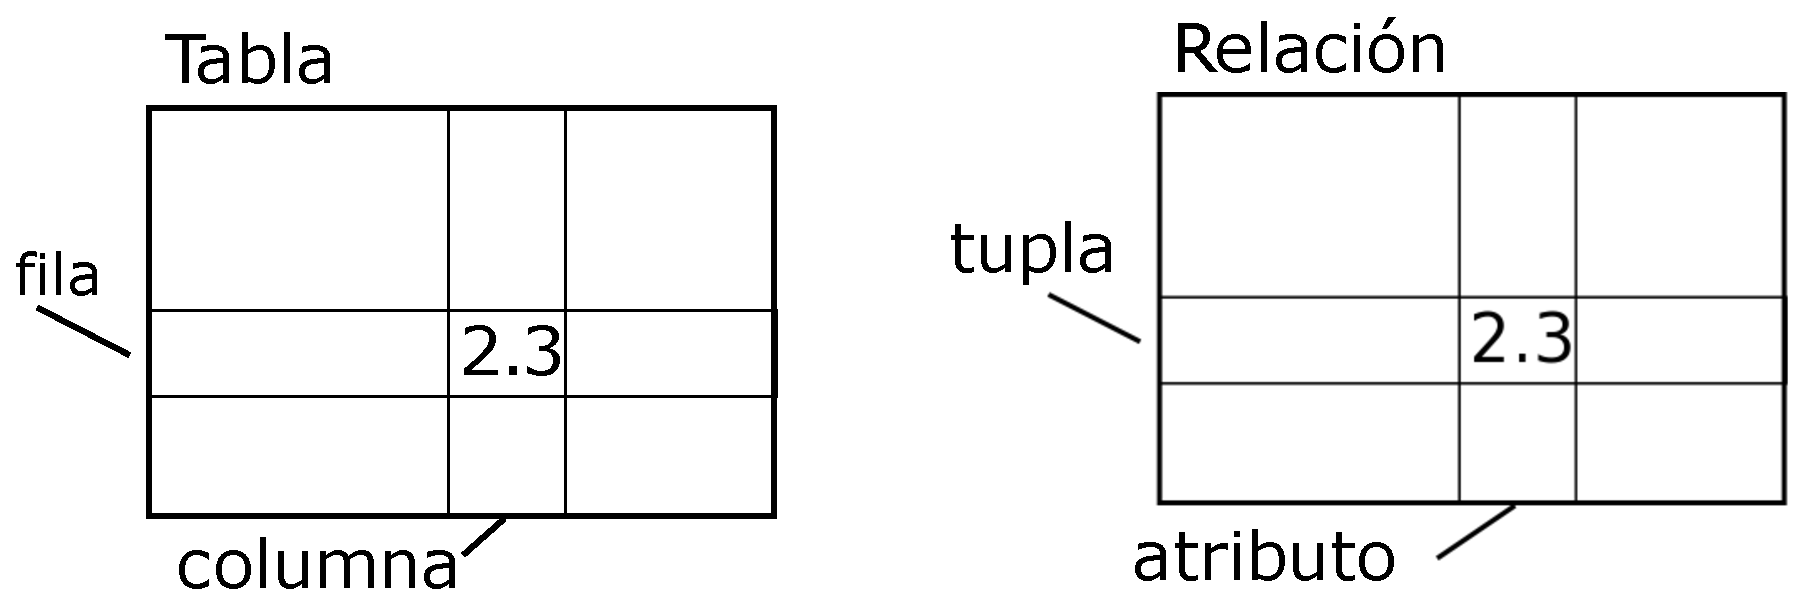
\includegraphics[height=1.50in]{figs2/relational.eps}}
\afterfig

En las descripciones técnicas de las bases de datos relacionales, los conceptos de
tabla, fila y columna reciben los nombres más formales
de {\bf relación}, {\bf tupla}, y {\bf atributo} respectivamente.
Nosotros a lo largo de este capítulo usaremos los términos menos formales.

\section{Add-on de Firefox para gestión de SQLite}

A pesar de que en este capítulo nos centraremos en el uso de Python para trabajar con datos
en archivos de bases de datos SQLite, hay muchas operaciones que pueden realizarse
de forma más eficaz usando un add-on para Firefox llamado {\bf SQLite
Database Manager}, que se puede descargar libremente desde:

\url{https://addons.mozilla.org/en-us/firefox/addon/sqlite-manager/}

Utilizando el navegador se pueden crear tablas con facilidad, insertar y editar datos
o ejecutar consultas SQL sencillas sobre la base de datos.

En cierto sentido, el gestor de base de datos es parecido a un editor de texto
que trabaja con archivos de texto. Cuando quieres realizar uno o
dos cambios en un archivo de texto, lo más sencillo es abrirlo en
un editor de texto y realizar los cambios que quieres. Cuando debes realizar
muchas modificaciones en el archivo, a menudo
habrá que escribir un programa en Python sencillo. El mismo enfoque
se puede aplicar al trabajo con bases de datos. Se realizarán las
operaciones más sencillas en el gestor de bases de datos, y para otras más complejas
será más conveniente usar Python.

\section{Creación de una tabla en una base de datos}

Las bases de datos necesitan una estructura más definida que las listas
o diccionarios de Python\footnote{SQLite en realidad permite cierta
flexibilidad respecto al tipo de datos que se almacenan en cada columna,
pero en este capítulo nosotros vamos a mantener los tipos de datos estrictos
para que los conceptos que aprendamos puedan ser igualmente aplicados a otras
bases de datos como MySQL.}.

Cuando se crea una {\bf tabla}, se debe
indicar de antemano a la base de datos los nombres de cada una de las
{\bf columnas} de la tabla y el tipo de datos que se van a
almacenar en cada {\bf columna}. Cuando el software de la base de datos
conoce el tipo de datos de cada columna, puede elegir el modo más
eficiente de almacenar y buscar en ellas, de acuerdo al tipo de
datos guardados.

Puedes revisar los distintos tipos de datos soportados por SQLite
en la siguiente dirección:

\url{http://www.sqlite.org/datatypes.html}

El tener que definir de antemano una estructura para los datos puede parecer incómodo
al principio, pero la recompensa consiste en obtener un acceso rápido a los datos,
incluso cuando la base de datos contiene una gran cantidad de ellos.

El código para crear un archivo de base de datos y una tabla
llamada {\tt Canciones} con dos columnas en la
base de datos es el siguiente:

\index{sqlite3, módulo}
\index{módulo!sqlite3}
\beforeverb
\begin{verbatim}
import sqlite3

conn = sqlite3.connect('musica.sqlite3')
cur = conn.cursor()

cur.execute('DROP TABLE IF EXISTS Canciones ')
cur.execute('CREATE TABLE Canciones (titulo TEXT, reproducciones INTEGER)')

conn.close()
\end{verbatim}
\afterverb
%
\index{connect, función}
\index{función!connect}
\index{cursor, función}
\index{función!cursor}
La operación {\tt connect} realiza una ``conexión'' con la base de datos
almacenada en el archivo {\tt musica.sqlite3} del directorio actual. Si
el archivo no existe, se creará nuevo. La razón de que se le
llame una ``conexión'' es que a veces la base de datos se almacena en
un ``servidor de bases de datos'', distinto del servidor en el cual está
funcionando nuestra aplicación. En nuestros ejemplos, dado que son sencillos,
la base de datos será simplemente un archivo local en el mismo directorio
en el que está funcionando el código de Python.

Un {\bf cursor} es como un manejador de fichero, y se puede usar para realizar
operaciones en los datos almacenados en la base de datos. La llamada a
{\tt cursor()} es muy parecida conceptualmente a la llamada a
{\tt open()} cuando se está tratando con ficheros de texto.

\beforefig
\centerline{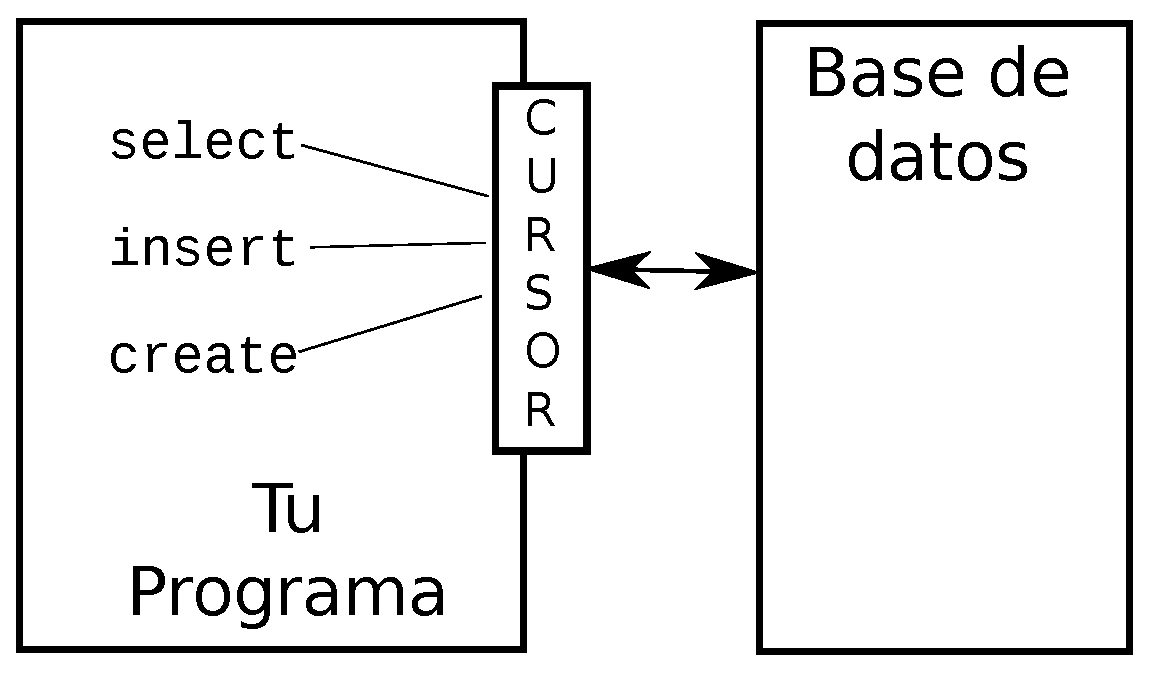
\includegraphics[height=1.50in]{figs2/cursor.eps}}
\afterfig

Una vez que tenemos el cursor, podemos comenzar a ejecutar
comandos sobre el contenido de la base de datos, usando el método
{\tt execute()}.

Los comandos de las bases de datos se expresan en un lenguaje especial que ha
sido estandarizado entre varios proveedores de bases de datos diferentes
para permitirnos aprender un único lenguaje para todas ellas. Este lenguaje
recibe el nombre de {\bf Lenguaje de Consultas eStructurado}, o {\bf SQL}
por sus iniciales en inglés.

\url{http://en.wikipedia.org/wiki/SQL}

En nuestro ejemplo, estamos ejecutando dos comandos SQL sobre la base de datos.
Por convención, mostraremos las palabras claves de SQL en mayúscula
y las partes de los comandos que añadamos nosotros (como los nombres
de las tablas y las columnas) irán en minúsculas.

El primer comando SQL elimina la tabla {\tt Canciones} de la
base de datos si ya existe. Este planteamiento se utiliza simplemente para permitirnos
ejecutar el mismo programa para crear la tabla {\tt Canciones} una y
otra vez sin provocar un error. Fíjate en que el comando
{\tt DROP TABLE} borra la tabla y todo su contenido
de la base de datos (es decir, aquí no existe la opción ``deshacer'').

\beforeverb
\begin{verbatim}
cur.execute('DROP TABLE IF EXISTS Canciones ')
\end{verbatim}
\afterverb
%
El segundo comando crea un tabla llamada
{\tt Canciones} con una columna de texto llamada {\tt titulo}
y una columna de enteros llamada {\tt reproducciones}.

\beforeverb
\begin{verbatim}
cur.execute('CREATE TABLE Canciones (titulo TEXT, reproducciones INTEGER)')
\end{verbatim}
\afterverb
%
Ahora que ya hemos creado la tabla llamada {\tt Canciones}, podemos guardar
algunos datos en ella usando la operación de SQL {\tt INSERT}. Empezaremos
realizando otra vez una conexión con la base de datos y obteniendo el {\tt cursor}.
Luego podremos ejecutar comandos SQL utilizando ese cursor.

El comando {\tt INSERT} de SQL indica qué tabla se está utilizando
y luego define una fila nueva, enumerando los campos que se desean
incluir {\tt (título, reproducciones)}, seguidos por los {\tt valores (VALUES)} que
se desean colocar en esa fila. Nosotros vamos a especificar los valores como signos de interrogación
{\tt (?, ?)} para indicarle que los valores reales serán pasados como una
tupla {\tt ( 'My Way', 15 ) } en el segundo parámetro de la
llamada a {\tt execute()}.

\beforeverb
\begin{verbatim}
import sqlite3

conn = sqlite3.connect('musica.sqlite3')
cur = conn.cursor()

cur.execute('INSERT INTO Canciones (titulo, reproducciones) VALUES ( ?, ? )', 
    ( 'Thunderstruck', 20 ) )
cur.execute('INSERT INTO Canciones (titulo, reproducciones) VALUES ( ?, ? )', 
    ( 'My Way', 15 ) )
conn.commit()

print 'Canciones:'
cur.execute('SELECT titulo, reproducciones FROM Canciones')
for fila in cur :
   print fila

cur.execute('DELETE FROM Canciones WHERE reproducciones < 100')
conn.commit()

cur.close()
\end{verbatim}
\afterverb
%
Primero {\tt insertamos (INSERT)} dos filas en la tabla y usamos {\tt commit()}
para forzar a que los datos sean escritos en el archivo de la base de datos.

\beforefig
\centerline{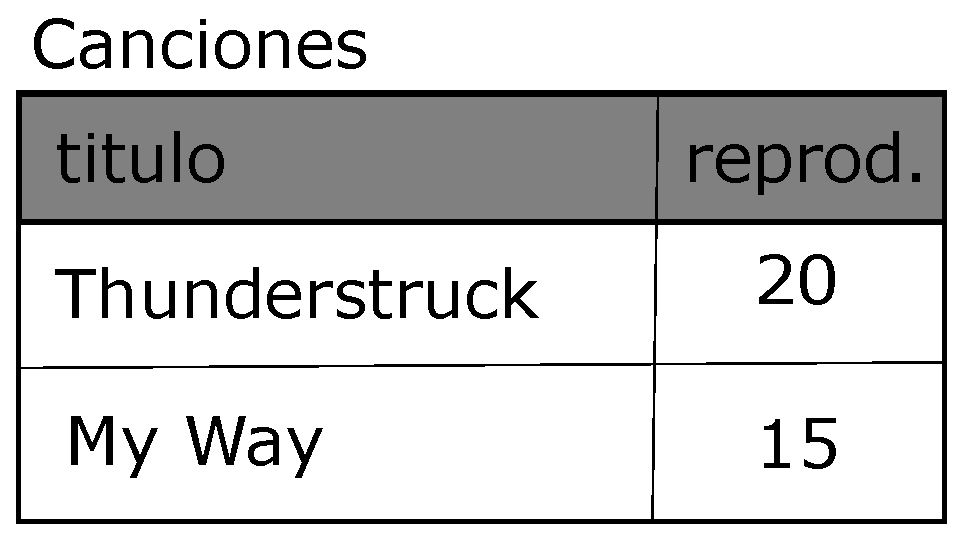
\includegraphics[height=1.00in]{figs2/tracks.eps}}
\afterfig

Después usamos el comando {\tt SELECT} para
recuperar las filas que acabamos de insertar en la tabla.
En el comando
{\tt SELECT}, indicamos qué columnas nos gustaría obtener {\tt (titulo, reproducciones)}
e indicamos desde qué tabla queremos recuperar los datos. Después de
ejecutar la sentencia {\tt SELECT}, el cursor se convierte en algo con lo que podemos
iterar mediante una sentencia {\tt for}. Por eficiencia,
el cursor no lee todos los datos de la base de datos
cuando se ejecuta la sentencia {\tt SELECT}.
En lugar de ello, los datos van siendo leídos según
se van pidiendo las filas desde el bucle creado con la sentencia {\tt for}.

La salida del programa es la siguiente:

\beforeverb
\begin{verbatim}
Canciones:
(u'Thunderstruck', 20)
(u'My Way', 15)
\end{verbatim}
\afterverb
%
\index{Unicode}
Nuestro bucle {\tt for} encuentra dos filas, y cada fila es una tupla de Python cuyo
primer valor es el {\tt título} y el segundo es el número de {\tt reproducciones}.
No nos preocupa que la cadena del título comience por
{\tt u'}. Se trata de una indicación de que las cadenas son del tipo {\bf Unicode},
y por tanto capaces de almacenar conjuntos de caracteres no-latinos.

Al final del programa, ejecutamos un comando SQL para {\tt borrar (DELETE)}
las filas que acabamos de crear, de modo que podamos ejecutar el programa una y otra vez.
El comando {\tt DELETE} nos muestra el uso de la cláusula {\tt WHERE}, la cual
nos permite expresar un criterio de selección, de modo que podemos pedir a la base de datos
que aplique el comando solamente a las filas que cumplan ese criterio. En este ejemplo,
el criterio es cumplido por todas las filas, así que vaciamos la tabla
para que podamos ejecutar el programa de nuevo repetidamente. Después de que se ha realizado el
{\tt DELETE}, llamamos de nuevo a {\tt commit()} para forzar a los datos a ser eliminados de
la base de datos.

\section{Resumen de Lenguaje de Consultas Estructurado}

Hasta ahora, hemos estado usando el Lenguaje de Consultas Estructurado en nuestros
ejemplos de Python y hemos utilizado muchos de los comandos básicos de SQL.
En esta sección, nos centraremos en el lenguaje SQL en particular
y echaremos un vistazo a su sintaxis.

A pesar de que hay muchos proveedores de bases de datos, el Lenguaje de Consultas
eStructurado (SQL) está estandarizado, de modo que podríamos comunicarnos de una forma
similar con sistemas de bases de datos de múltiples vendedores. 

Una base de datos relacional está compuesta por tablas, filas y columnas. Las columnas
tienen generalmente un tipo de datos que puede ser texto, numérico, o fecha. Cuando se crea
una tabla, se indican los nombres y tipos de cada columna.

\beforeverb
\begin{verbatim}
CREATE TABLE Canciones (titulo TEXT, reproducciones INTEGER)
\end{verbatim}
\afterverb
%
Para insertar una fila en una tabla, usamos el comando de SQL {\tt INSERT}:

\beforeverb
\begin{verbatim}
INSERT INTO Canciones (titulo, reproducciones) VALUES ('My Way', 15)
\end{verbatim}
\afterverb
%
La sentencia {\tt INSERT} especifica el nombre de la tabla, seguido por una lista
de los campos/columnas que se quieren establecer en la fila nueva, a continuación
la palabra clave {\tt VALUES} y una lista de los valores correspondientes
para cada uno de los campos.

El comando de SQL {\tt SELECT} se usa para recuperar filas y columnas desde una base de datos.
La sentencia {\tt SELECT} permite especificar qué columnas se quieren
recibir, junto con una clausula {\tt WHERE} para indicar qué 
filas se desean obtener. También permite una clausula opcional,
{\tt ORDER BY} para controlar el orden de las filas devueltas.

\beforeverb
\begin{verbatim}
SELECT * FROM Canciones WHERE titulo = 'My Way'
\end{verbatim}
\afterverb
%
El \verb"*" indica que se desea que la base de datos devuelva todas las
columnas para cada línea que cumpla la condición de la clausula {\tt WHERE}.

Fíjate que, a diferencia de lo que ocurre en Python, en SQL la clausula {\tt WHERE}
utiliza un único signo igual
para indicar una comprobación de igualdad, en lugar de utilizar un signo doble igual.
Otras operaciones lógicas que se permiten en una clausula {\tt WHERE} son
\verb"<",
\verb">",
\verb"<=",
\verb">=",
\verb"!=",
junto con {\tt AND}, {\tt OR} y paréntesis
para construir expresiones lógicas.

Se puede solicitar que las columnas devueltas vengan ordenadas por uno
de los campos así:

\beforeverb
\begin{verbatim}
SELECT titulo, reproducciones FROM Canciones ORDER BY titulo
\end{verbatim}
\afterverb
%
Para eliminar una fila, es necesario usar una clausula {\tt WHERE} en una sentencia
{\tt DELETE} de SQL. La clausula {\tt WHERE} determina qué filas serán eliminadas:

\beforeverb
\begin{verbatim}
DELETE FROM Canciones WHERE titulo = 'My Way'
\end{verbatim}
\afterverb
%
Es posible {\tt actualizar (UPDATE)} una columna o varias de una o más filas
en una tabla usando la sentencia de SQL {\tt UPDATE}, como se muestra a continuación:

\beforeverb
\begin{verbatim}
UPDATE Canciones SET reproducciones = 16 WHERE titulo = 'My Way'
\end{verbatim}
\afterverb
%
La sentencia {\tt UPDATE} especifica una tabla y a continuación
una lista de campos y valores a cambiar detrás de la palabra
clave {\tt SET}, y finalmente una clausula opcional {\tt WHERE} para elegir
las filas que van a ser actualizadas. Una única sentencia {\tt UPDATE}
cambiará todas las filas que coincidan con la clausula {\tt WHERE}.
Si no se ha especificado ninguna clausula {\tt WHERE}, se realizará la
{\tt actualización} de todas las filas de la tabla.

Existen cuatro comandos básicos de SQL (INSERT, SELECT, UPDATE y DELETE), que
nos permiten realizar las cuatro operaciones básicas necesarias para crear y mantener datos.

\section{Rastreo en Twitter usando una base de datos}

En esta sección, crearemos un programa araña sencillo que se moverá
a través de cuentas de Twitter y construirá una base de datos de ellas.
\emph{Nota: Ten mucho cuidado al ejecutar este programa. Si extraes
demasiados datos o ejecutas el programa durante demasiado tiempo
pueden terminar cortándote el acceso a Twitter.}

Uno de los problemas de cualquier tipo de programa araña es que se
necesita poderlo detener y volver a poner en marcha muchas veces, y
no se quieren perder los datos que se hayan recuperado hasta ese momento.
No querrás tener que empezar siempre la recuperación de datos desde
el principio, de modo que necesitaremos almacenar los datos según los vamos recuperando para
que nuestro programa pueda usar esa copia de seguridad y continuar de nuevo su recogida de datos
donde lo dejó la última vez.

Empezaremos por recuperar los amigos de Twitter de una persona y sus estados,
moviéndonos a través de la lista de amigos y añadiendo cada uno de ellos
a la base de datos para poder recuperarlos en el futuro. Después
de haber procesado todos los amigos de esa persona, consultaremos la base de datos
y recuperaremos los amigos de uno de esos amigos. Continuaremos haciendo esto una y otra vez,
recogiendo cualquier persona ``no visitada'', recuperando su lista de amigos
y añadiendo aquellos que no tengamos ya en nuestra lista para una próxima visita.

También rastrearemos cuántas veces hemos visto un amigo concreto en la
base de datos para tener una idea de su ``popularidad''.

Como estamos almacenando nuestra lista de cuentas de conocidos,
cuándo hemos recuperado una cuenta o no
y la popularidad de cada cuenta
en una base datos en el disco del ordenador,
podremos detener y reanudar el programa tantas veces como queramos. 

% POR HACER: Añadir una referencia al lugar correcto
Este programa es un poco complejo. Está basado en el código
de un ejercicio anterior del libro que usa la
API de Twitter.

Aquí está el código fuente para nuestra aplicación araña de Twitter:

\beforeverb
\begin{verbatim}
import urllib
import twurl
import json
import sqlite3

TWITTER_URL = 'https://api.twitter.com/1.1/friends/list.json'

conn = sqlite3.connect('arana.sqlite3')
cur = conn.cursor()

cur.execute('''
CREATE TABLE IF NOT EXISTS Twitter 
(nombre TEXT, recuperado INTEGER, amigos INTEGER)''')

while True:
    cuenta = raw_input('Introduce una cuenta de Twitter o salir: ')
    if ( cuenta == 'salir' ) : break
    if ( len(cuenta) < 1 ) :
        cur.execute('SELECT nombre FROM Twitter WHERE recuperado = 0 LIMIT 1')
        try:
            cuenta = cur.fetchone()[0]
        except:
            print 'No se han encontrado cuentas de Twitter por recuperar'
            continue

    url = twurl.augment(TWITTER_URL, 
               {'screen_name': cuenta, 'count': '20'} )
    print 'Recuperando', url
    conexion = urllib.urlopen(url)
    datos = conexion.read()
    cabeceras = conexion.info().dict
    # print 'Restante', cabeceras['x-rate-limit-remaining']
    js = json.loads(data)
    # print json.dumps(js, indent=4)

    cur.execute('UPDATE Twitter SET recuperado=1 WHERE nombre = ?', (cuenta, ) )

    contnuevas = 0
    contantiguas = 0
    for u in js['users'] :
        amigo = u['screen_name']
        print amigo
        cur.execute('SELECT amigos FROM Twitter WHERE nombre = ? LIMIT 1', 
            (amigo, ) )
        try:
            contador = cur.fetchone()[0]
            cur.execute('UPDATE Twitter SET amigos = ? WHERE nombre = ?', 
                (contador+1, amigo) )
            contantiguas = contantiguas + 1
        except:
            cur.execute('''INSERT INTO Twitter (nombre, recuperado, amigos) 
                VALUES ( ?, 0, 1 )''', ( amigo, ) )
            contnuevas = contnuevas + 1
    print 'Cuentas nuevas=',contnuevas,' ya visitadas=',contantiguas
    conn.commit()

cur.close()
\end{verbatim}
\afterverb
%
Nuestra base de datos está almacenada en el archivo {\tt arana.sqlite3} y tiene
una tabla llamada {\tt Twitter}. Cada fila en la tabla {\tt Twitter}
contiene una columna para el nombre de la cuenta, otra para indicar si hemos recuperado los
amigos de esa cuenta, y otra para guardar cuántas veces se ha visto esa cuenta añadida en
la lista de amigos de las demás.

En el bucle principal del programa, pedimos al usuario el nombre de una cuenta
de Twitter o ``salir'' para finalizar el programa.
Si el usuario introduce una cuenta de Twitter, recuperamos la
lista de amigos de ese usuario y sus estados,
y añadimos cada amigo a la base de datos si no
estaba ya en ella. Si el amigo ya está en la lista,
aumentamos en 1 el campo {\tt amigos} en la fila de la base de datos correspondiente.

Si el usuario pulsa intro, buscamos en la base de datos la siguiente
cuenta de Twitter que no haya sido aún recuperada, recuperamos los
amigos de esa cuenta y sus estados, y luego los añadimos a la base de datos
o los actualizamos, e incrementamos su contador de {\tt amigos}.

Una vez hemos recuperado la lista de amigos y sus estados, nos movemos
a través de los elementos {\tt users} del JSON devuelto
y recuperamos el \verb"screen_name" (nombre a mostrar) de cada usuario. Luego usamos
la sentencia {\tt SELECT} para comprobar si ya tenemos almacenado ese
nombre concreto en la base de datos y si es así recuperamos su
contador de amigos ({\tt amigos}).

\beforeverb
\begin{verbatim}
    contnuevas = 0
    contantiguas = 0
    for u in js['users'] :
	    amigo = u['screen_name']
	    print amigo
	    cur.execute('SELECT amigos FROM Twitter WHERE nombre = ? LIMIT 1', 
		    (amigo, ) )
	    try:
		    contador = cur.fetchone()[0]
		    cur.execute('UPDATE Twitter SET amigos = ? WHERE nombre = ?', 
			    (contador+1, amigo) )
		    contantiguas = contantiguas + 1
		except:
		    cur.execute('''INSERT INTO Twitter (nombre, recuperado, amigos) 
			    VALUES ( ?, 0, 1 )''', ( amigo, ) )
		    contnuevas = contnuevas + 1
    print 'Cuentas nuevas=',contnuevas,' ya visitadas=',contantiguas
    conn.commit()
\end{verbatim}
\afterverb
%
Una vez que el cursor ejecuta la sentencia {\tt SELECT},
debemos recuperar las filas. Podríamos hacerlo con una sentencia {\tt for},
pero dado que sólo estamos recuperando una única fila
({\tt LIMIT 1}), podemos también usar el método {\tt fetchone()} para extraer
la primera (y única) fila que da como resultado la operación {\tt SELECT}.
Dado que {\tt fetchone()} devuelve la fila como una {\bf tupla} (incluso si sólo
contiene un campo), tomamos el primer valor de la tupla mediante {\tt [0]}, para
almacenar así dentro de la variable {\tt contador} el valor del contador de amigos actual.

Si esta operación tiene éxito, usamos la sentencia {\tt UPDATE} de SQL con una
clausula {\tt WHERE} para añadir 1 a la columna {\tt amigos} de aquella fila que
coincida con la cuenta del amigo. Fíjate que hay dos marcadores de posición (es decir,
signos de interrogación) en el SQL, y que el segundo parámetro de {\tt execute()} es
una tupla de dos elementos que contiene los valores que serán sustituidos por esas
interrogaciones dentro de la sentencia SQL.

Si el código en el bloque {\tt try} falla, se deberá probablemente a que ningún registro
coincide con lo especificado en la clausula {\tt WHERE nombre = ?} de la sentencia SELECT.
Así que en el bloque {\tt except}, usamos la sentencia de SQL {\tt INSERT} para añadir el
nombre a mostrar (\verb"screen_name") del amigo a la tabla con una indicación de que no lo hemos
recuperado aún y fijamos su contador de amigos a cero.

La primera vez que el programa funciona e introducimos una cuenta de Twitter, mostrará
algo similar a esto:

\beforeverb
\begin{verbatim}
Introduce una cuenta de Twitter o salir: drchuck
Recuperando http://api.twitter.com/1.1/friends ...
Cuentas nuevas= 20  ya visitadas= 0
Introduce una cuenta de Twitter o salir: salir
\end{verbatim}
\afterverb
%
Dado que es la primera vez que ejecutamos el programa, la base de datos
está vacía, así que creamos el fichero {\tt arana.sqlite3} y añadimos
una tabla llamada {\tt Twitter} a la base de datos. A continuación
recuperamos algunos amigos y los añadimos a la base de datos, ya que
ésta está vacía.

En este momento, tal vez sea conveniente escribir un extractor de datos sencillo
para echar un vistazo a lo que hay dentro del fichero {\tt arana.sqlite3}:

\beforeverb
\begin{verbatim}
import sqlite3

conn = sqlite3.connect('arana.sqlite3')
cur = conn.cursor()
cur.execute('SELECT * FROM Twitter')
contador = 0
for fila in cur :
   print fila
   contador = contador + 1
print contador, 'filas.'
cur.close()
\end{verbatim}
\afterverb
%
Este programa simplemente abre la base de datos y selecciona todas las columnas
de todas las filas de la tabla {\tt Twitter}, luego
se mueve a través de las filas e imprime en pantalla su contenido.

Si lanzamos este programa después de la primera ejecución de nuestra araña
de Twitter, la salida que mostrará será similar a ésta:

\beforeverb
\begin{verbatim}
(u'opencontent', 0, 1)
(u'lhawthorn', 0, 1)
(u'steve_coppin', 0, 1)
(u'davidkocher', 0, 1)
(u'hrheingold', 0, 1)
...
20 filas.
\end{verbatim}
\afterverb
%
Vemos una fila para cada nombre, que aún no hemos
recuperado los datos de ninguno de esos nombres, y
que todo el mundo en la base de datos tiene un amigo.

En este momento la base de datos muestra la recuperación de los amigos de
nuestra primera cuenta de Twitter ({\bf drchuck}). Podemos ejecutar de nuevo
el programa y pedirle que recupere los amigos de la siguiente
cuenta ``sin procesar'', simplemente pulsando intro en vez de
escribir el nombre de una cuenta:

\beforeverb
\begin{verbatim}
Introduce una cuenta de Twitter o salir:  
Recuperando http://api.twitter.com/1.1/friends ...
Cuentas nuevas= 18  ya visitadas= 2
Introduce una cuenta de Twitter o salir: 
Recuperando http://api.twitter.com/1.1/friends ...
Cuentas nuevas= 17  ya visitadas= 3
Introduce una cuenta de Twitter o salir: salir
\end{verbatim}
\afterverb
%
Como hemos pulsado intro (es decir, no hemos especificado otra cuenta de Twitter),
se ha ejecutado el código siguiente:

\beforeverb
\begin{verbatim}
    if ( len(cuenta) < 1 ) :
        cur.execute('SELECT nombre FROM Twitter WHERE recuperado = 0 LIMIT 1')
        try:
            cuenta = cur.fetchone()[0]
        except:
            print 'No se han encontrado cuentas de Twitter por recuperar'
            continue
\end{verbatim}
\afterverb
%
Usamos la sentencia de SQL {\tt SELECT} para recuperar el nombre del primer
usuario ({\tt LIMIT 1}) que aún tiene su valor de ``hemos recuperado ya este usuario''
a cero. También usamos el modelo {\tt fechone()[0]} en un bloque
try/except para extraer el nombre de los datos recuperados o bien
mostrar un mensaje de error y volver al principio.

Si hemos recuperado con éxito el nombre de una cuenta que aún no había sido procesada,
tratamos sus datos de este modo:

\beforeverb
\begin{verbatim}
    url = twurl.augment(TWITTER_URL, {'screen_name': cuenta, 'count': '20'} )
    print 'Recuperando', url
    conexion = urllib.urlopen(url)
    datos = conexion.read()
    js = json.loads(datos)

    cur.execute('UPDATE Twitter SET recuperado=1 WHERE nombre = ?', (cuenta, ) )
\end{verbatim}
\afterverb
%
Una vez recuperamos los datos correctamente, usamos la sentencia {\tt UPDATE}
para poner la columna {\tt recuperado} a 1, lo que indica que hemos terminado
la recuperación de amigos de esa cuenta. Esto impide que recuperemos los
mismos datos una y otra vez y nos permite ir avanzando a través de la red
de amigos de Twitter. 

Si ejecutamos el programa de amigos y pulsamos intro dos veces para recuperar
los amigos del siguiente amigo no visitado,
y luego ejecutamos de nuevo el programa de extracción de datos, nos mostrará la
salida siguiente: 

\beforeverb
\begin{verbatim}
(u'opencontent', 1, 1)
(u'lhawthorn', 1, 1)
(u'steve_coppin', 0, 1)
(u'davidkocher', 0, 1)
(u'hrheingold', 0, 1)
...
(u'cnxorg', 0, 2)
(u'knoop', 0, 1)
(u'kthanos', 0, 2)
(u'LectureTools', 0, 1)
...
55 rows.
\end{verbatim}
\afterverb
%
Podemos ver que se han guardado correctamente las visitas que hemos realizado a
a {\tt lhawthorn} y {\tt opencontent}. Además las cuentas
{\tt cnxorg} y {\tt kthanos} ya tienen dos seguidores.
A pesar de hasta ahora hemos recuperados sólo los amigos de tres personas
({\tt drchuck}, {\tt opencontent}, y {\tt lhawthorn}), la tabla contiene ya
55 filas de amigos por recuperar.

Cada vez que ejecutamos el programa y pulsamos intro, se elegirá la siguiente
cuenta no visitada (es decir, ahora la siguiente cuenta sería \verb"steve_coppin"),
recuperará sus amigos, los marcará como recuperados, y para cada uno de los
amigos de \verb"steve_coppin" o bien lo añadirá al final de la
base de datos o bien actualizará su contador de amigos si ya estaba en la
tabla.

Como ves, al estar los datos del programa almacenados en el disco en una base de datos,
la actividad de rastreo puede ser suspendida y reanudada tantas veces como se desee
sin que se produzca ninguna pérdida de datos.

\section{Modelado de datos básico}

La potencia real de las bases de datos relacionales se manifiesta cuando se construyen múltiples
tablas y se crean enlaces entre ellas. El acto de decidir cómo separar los datos de tu
aplicación en múltiples tablas y establecer las relaciones
entre esas tablas recibe el nombre de {\bf modelado de datos}. El
documento de diseño que muestra las tablas y sus relaciones
se llama {\bf modelo de datos}.

El modelado de datos es una habilidad relativamente sofisticada, y en esta sección sólo
introduciremos los conceptos más básicos acerca de ello. Para obtener más
detalles sobre modelado de datos puedes comenzar con:

\url{http://en.wikipedia.org/wiki/Relational_model}

Supongamos que para nuestra aplicación de rastreo de Twitter, en vez de contar
los amigos de una persona sin más, queremos mantener una lista de
todas las relaciones entre ellos, de modo que podamos encontrar una lista de
gente que esté siguiendo la cuenta de una persona concreta.

Dado que todo el mundo puede tener potencialmente muchas cuentas siguiéndole,
no podemos añadir simplemente una única columna a nuestra tabla de {\tt Twitter}.
De modo que creamos una tabla nueva que realice un seguimiento de parejas de amigos.
A continuación se muestra un modo sencillo de hacer una tabla de este tipo:

\beforeverb
\begin{verbatim}
CREATE TABLE Camaradas (desde_amigo TEXT, hacia_amigo TEXT)
\end{verbatim}
\afterverb
%
Cada vez que encontremos a una persona de las que está siguiendo {\tt drchuck},
insertaremos una fila de esta forma:

\beforeverb
\begin{verbatim}
INSERT INTO Camaradas (desde_amigo, hacia_amigo) VALUES ('drchuck', 'lhawthorn')
\end{verbatim}
\afterverb
%
Según vayamos procesando los 20 amigos de {\tt drchuck}
que nos envía Twitter, insertaremos 20 registros con ``drchuck''
como primer parámetro, de modo que terminaremos duplicando la
cadena un montón de veces en la base de datos.

Esta duplicación de cadenas de datos viola una de las mejores prácticas
para la {\bf normalización de bases de datos}, que básicamente consiste en
que nunca se debe guardar la misma cadena de datos más de una vez en la base de datos.
Si se necesitan los datos varias veces, se debe crear una
{\bf clave} numérica para ellos y hacer referencia a los datos reales
a través de esa clave.

En términos prácticos, una cadena ocupa un montón
de espacio más que un entero, tanto en el disco como en
la memoria del ordenador, y además necesita más tiempo de procesador
para ser comparada y ordenada. Si sólo se tienen unos pocos cientos de entradas,
el espacio y el tiempo de procesador no importan demasiado. Pero si se tienen
un millón de personas en la base de datos y la posibilidad de 100 millones
de enlaces de amigos, es importante ser capaz de revisar los datos tan rápido
como sea posible.

Nosotros vamos a almacenar nuestras cuentas de Twitter en una tabla llamada {\tt Personas}
en vez de hacerlo en la tabla {\tt Twitter} que usamos en el ejemplo anterior.
La tabla {\tt Personas} tiene una columna adicional
para almacenar la clave numérica asociada con la
fila de cada usuario de Twitter.
SQLite tiene una característica que permite añadir automáticamente el valor de la clave
para cualquier fila que insertemos en la tabla, usando un tipo especial de
datos en la columna, ({\tt INTEGER PRIMARY KEY}).

Podemos, pues, crear la tabla {\tt Personas} con esa columna adicional
{\tt id}, como se muestra a continuación:

\beforeverb
\begin{verbatim}
CREATE TABLE Personas
    (id INTEGER PRIMARY KEY, nombre TEXT UNIQUE, recuperado INTEGER)
\end{verbatim}
\afterverb
%
Fíjate que ya no necesitamos mantener un contador de amigos en cada columna
de la tabla {\tt Personas}.
Cuando elegimos {\tt INTEGER PRIMARY KEY} como el tipo de la columna {\tt id},
estamos indicando que queremos que SQLite controle esta columna y
asigne automáticamente una clave numérica única para cada fila que insertemos.
También añadimos la palabra clave {\tt UNIQUE} para indicar que no vamos
a permitir a SQLite insertar dos filas con el mismo valor de {\tt nombre}.

Ahora en vez de crear la tabla {\tt Camaradas} como hicimos antes, crearemos
una tabla llamada {\tt Seguimientos} con dos columnas de tipo entero,
\verb"desde_id" y \verb"hacia_id", y una restricción en la tabla que consistirá en que
la \emph{combinación} de \verb"desde_id" y \verb"hacia_id" deberá ser única
(es decir, no se podrán insertar filas en la tabla con estos valores duplicados).

\beforeverb
\begin{verbatim}
CREATE TABLE Seguimientos 
    (desde_id INTEGER, hacia_id INTEGER, UNIQUE(desde_id, hacia_id) )
\end{verbatim}
\afterverb
%
Cuando añadimos la claúsula {\tt UNIQUE} a nuestras tablas, estamos comunicando un conjunto
de reglas que vamos a exigir a la base de datos que se cumplan cuando se intenten insertar
registros. Estamos creando esas reglas porque le convienen a nuestro programa, como
veremos dentro de un momento. Ambas reglas impiden que se cometan errores y hacen
más sencillo escribir parte de nuestro código.

En esencia, al crear esta tabla {\tt Seguimientos}, estamos modelando una
``relación'', en la cual una persona ``sigue'' a otra
y se representa con un par de números que indican que (a) ambas personas están
conectadas y (b) la dirección de la relación.

\beforefig
\centerline{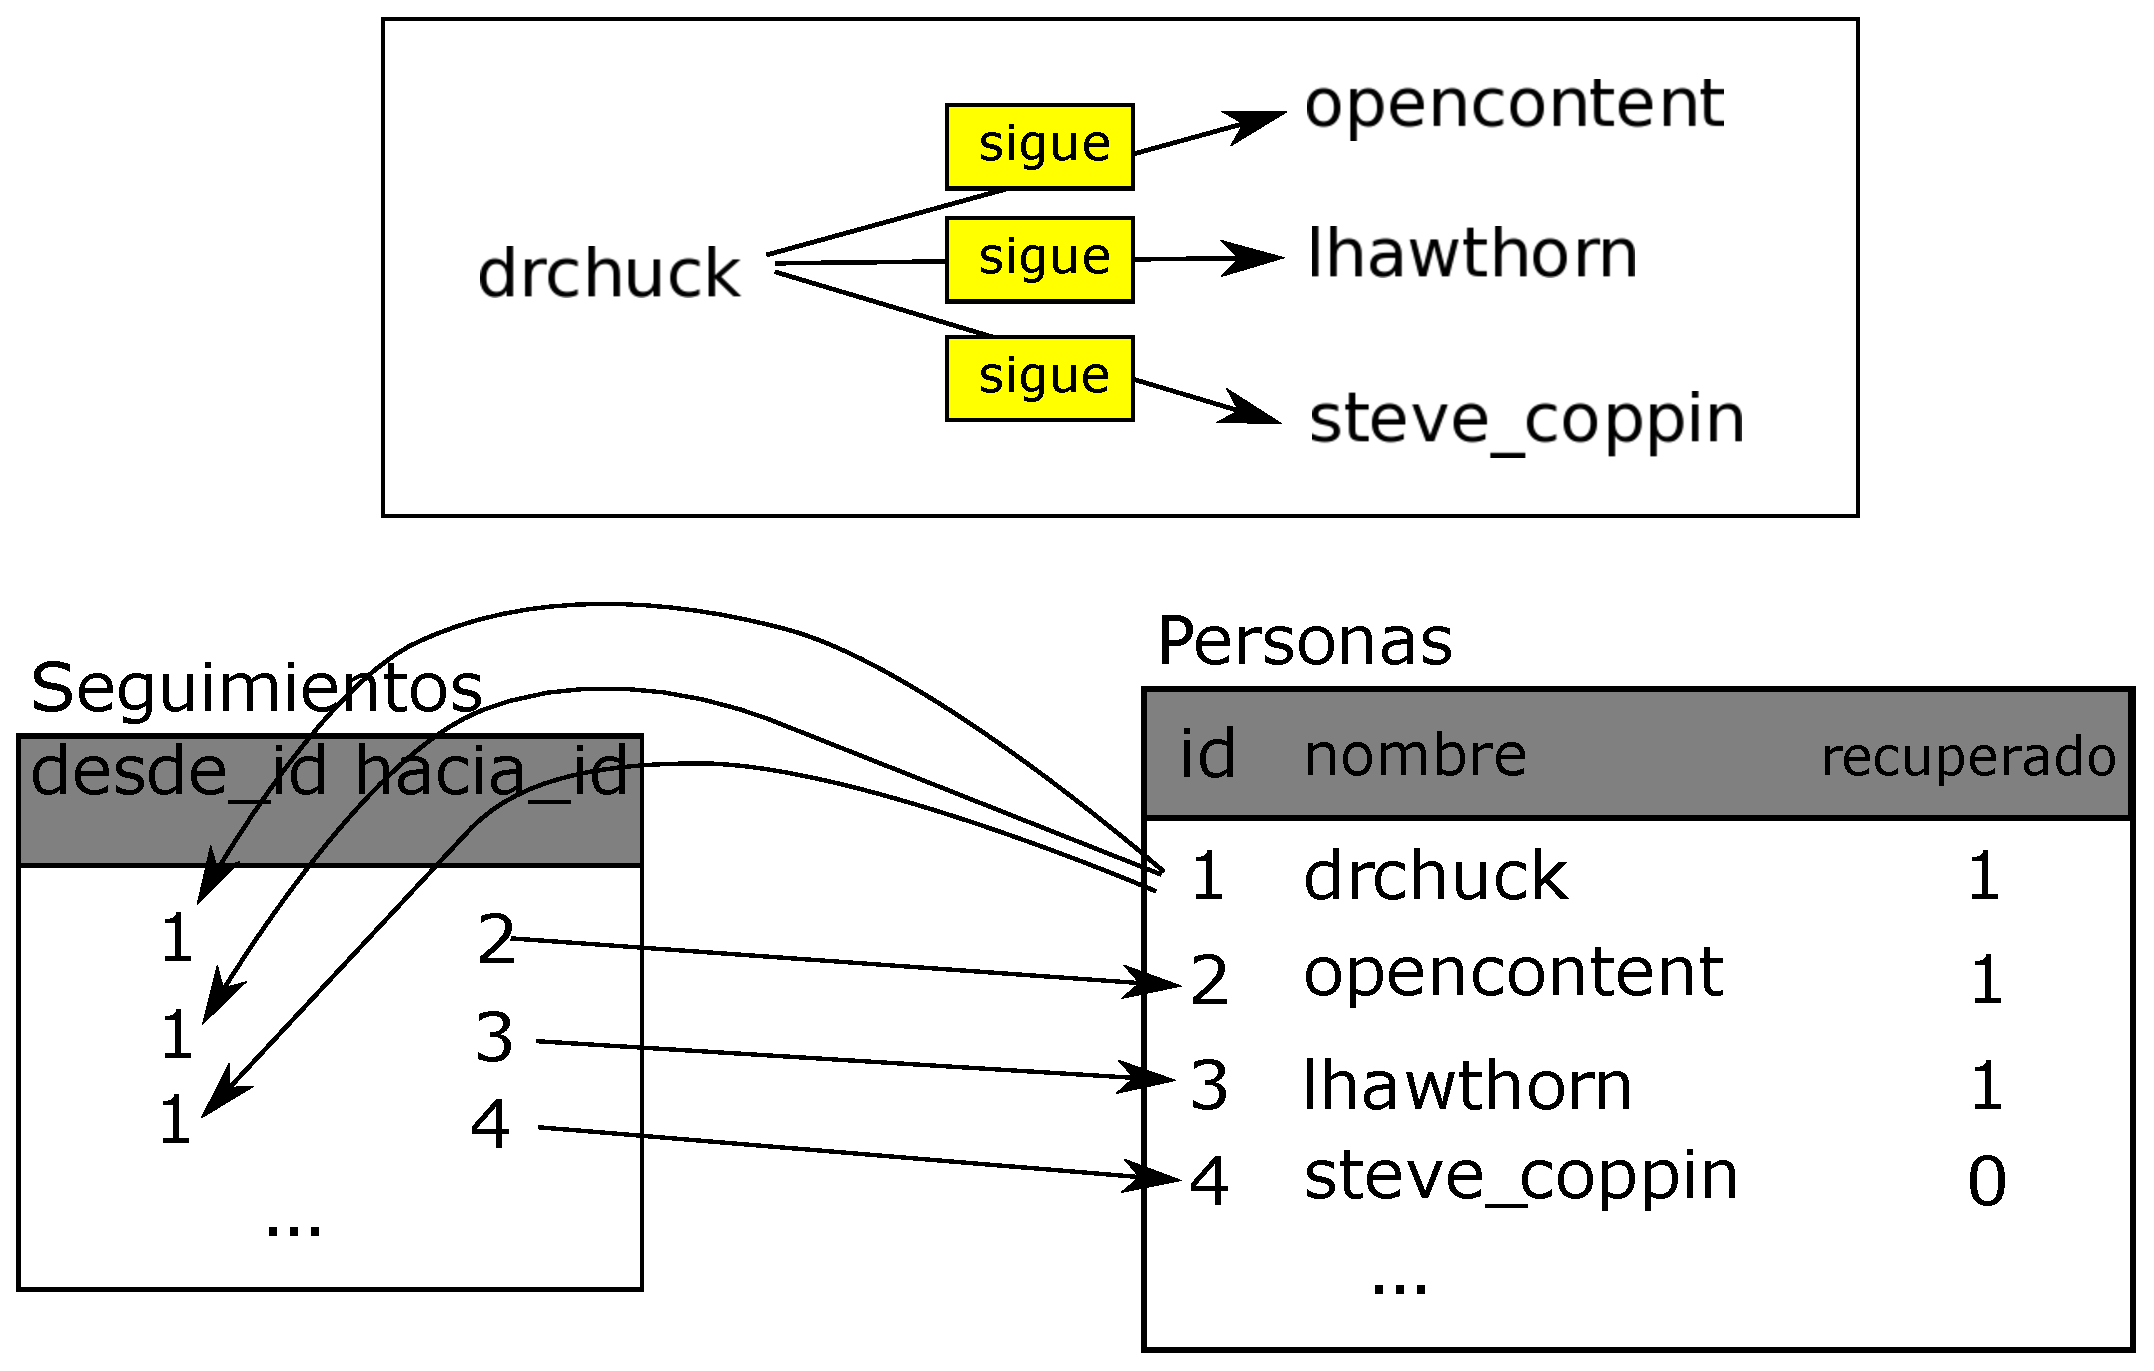
\includegraphics[height=2.50in]{figs2/twitter.eps}}
\afterfig


\section{Programación con múltiples tablas}

A continuación reharemos de nuevo el programa araña de Twitter usando dos tablas, las claves
primarias, y las claves de referencia, como hemos descrito antes. He aquí el código
de la nueva versión del programa:

\beforeverb
\begin{verbatim}
import urllib
import twurl
import json
import sqlite3

TWITTER_URL = 'https://api.twitter.com/1.1/friends/list.json'

conn = sqlite3.connect('amigos.sqlitesqlite3')
cur = conn.cursor()

cur.execute('''CREATE TABLE IF NOT EXISTS Personas 
    (id INTEGER PRIMARY KEY, nombre TEXT UNIQUE, recuperado INTEGER)''')
cur.execute('''CREATE TABLE IF NOT EXISTS Seguimientos 
    (desde_id INTEGER, hacia_id INTEGER, UNIQUE(desde_id, hacia_id))''')

while True:
    cuenta = raw_input('Introduce una cuenta de Twitter, o salir: ')
    if ( cuenta == 'salir' ) : break
    if ( len(cuenta) < 1 ) :
        cur.execute('''SELECT id, nombre FROM Personas
            WHERE recuperado = 0 LIMIT 1''')
        try:
            (id, cuenta) = cur.fetchone()
        except:
            print 'No se han encontrado cuentas de Twitter sin recuperar'
            continue
    else:
        cur.execute('SELECT id FROM Personas WHERE nombre = ? LIMIT 1', 
            (cuenta, ) )
        try:
            id = cur.fetchone()[0]
        except:
            cur.execute('''INSERT OR IGNORE INTO Personas (nombre, recuperado) 
                VALUES ( ?, 0)''', ( cuenta, ) )
            conn.commit()
            if cur.rowcount != 1 : 
                print 'Error insertando cuenta:',cuenta
                continue
            id = cur.lastrowid

    url = twurl.augment(TWITTER_URL, 
       {'screen_name': cuenta, 'count': '20'} )
    print 'Recuperando cuenta', cuenta
    conexion = urllib.urlopen(url)
    datos = conexion.read()
    cabeceras = conexion.info().dict
    print 'Restantes', cabeceras['x-rate-limit-remaining']

    js = json.loads(datos)
    # print json.dumps(js, indent=4)

    cur.execute('UPDATE Personas SET recuperado=1 WHERE nombre = ?', (cuenta, ) )

    contnuevas = 0
    contantiguas = 0
    for u in js['users'] :
        amigo = u['screen_name']
        print amigo
        cur.execute('SELECT id FROM Personas WHERE nombre = ? LIMIT 1', 
            (amigo, ) )
        try:
            amigo_id = cur.fetchone()[0]
            contantiguas = contantiguas + 1
        except:
            cur.execute('''INSERT OR IGNORE INTO Personas (nombre, recuperado) 
                VALUES ( ?, 0)''', ( amigo, ) )
            conn.commit()
            if cur.rowcount != 1 :
                print 'Error al insertar cuenta:',amigo
                continue
            amigo_id = cur.lastrowid
            contnuevas = contnuevas + 1
        cur.execute('''INSERT OR IGNORE INTO Seguimientos (desde_id, hacia_id) 
            VALUES (?, ?)''', (id, amigo_id) )
    print 'Cuentas nuevas=',contnuevas,' ya visitadas=',contantiguas
    conn.commit()

cur.close()
\end{verbatim}
\afterverb
%
Este programa empieza a resultar un poco complicado, pero ilustra
los patrones de diseño que debemos usar cuando utilizamos
claves de enteros para enlazar tablas. Esos patrones básicos son:

\begin{enumerate}

\item Crear tablas con claves primarias y restricciones.

\item Cuando tenemos una clave lógica para una persona (es decir, un
nombre de cuenta) y necesitamos el valor del {\tt id} de esa persona,
dependiendo de si esa persona ya está en la tabla
{\tt Personas} o no, tendremos que:
(1) buscar la persona en la tabla {\tt Personas} y
recuperar el valor de {\tt id} para esa persona,
o (2) añadir la persona a la tabla {\tt Personas} y obtener el
valor del {\tt id} para la fila recién añadida.

\item Insertar la fila que indica la relación de ``seguimiento''.

\end{enumerate}

Iremos explicando todos los puntos de uno en uno.

\subsection{Restricciones en tablas de bases de datos}

Una vez diseñada la estructura de la tabla, podemos indicar al sistema
de la base de datos que aplique unas cuantas reglas. Estas reglas nos
ayudarán a evitar errores y a introducir correctamente los datos en
las tablas. Cuando creemos nuestras tablas:

\beforeverb
\begin{verbatim}
cur.execute('''CREATE TABLE IF NOT EXISTS Personas 
    (id INTEGER PRIMARY KEY, nombre TEXT UNIQUE, recuperado INTEGER)''')
cur.execute('''CREATE TABLE IF NOT EXISTS Seguimientos 
    (desde_id INTEGER, hacia_id INTEGER, UNIQUE(desde_id, hacia_id))''')
\end{verbatim}
\afterverb
%
Estamos indicando que la columna {\tt nombre} de la tabla {\tt Personas} debe ser
{\tt UNIQUE} (única). Además indicamos que la combinación de los dos números
de cada fila de la tabla {\tt Seguimientos} debe ser también única. Estas restricciones
evitan que cometamos errores como añadir la misma relación entre las mismas personas
más de una vez.

Luego podemos aprovechar estas restricciones en el código siguiente:

\beforeverb
\begin{verbatim}
cur.execute('''INSERT OR IGNORE INTO Personas (nombre, recuperado) 
    VALUES ( ?, 0)''', ( amigo, ) )
\end{verbatim}
\afterverb
%
Aquí añadimos la clausula {\tt IGNORE} en la sentencia {\tt INSERT} para indicar
que si este {\tt INSERT} en concreto causara una violación de la regla
``el {\tt nombre} debe ser único'', el sistema de la base de datos está autorizado
a ignorar el {\tt INSERT}. De modo que estamos usando las restricciones de la base de datos
como una red de seguridad para asegurarnos de que no hacemos algo incorrecto de forma inadvertida.

De forma similar, el código siguiente se asegura de que no añadamos exactamente
la misma relación de {\tt Seguimiento} dos veces.

\beforeverb
\begin{verbatim}
cur.execute('''INSERT OR IGNORE INTO Seguimientos 
    (desde_id, hacia_id) VALUES (?, ?)''', (id, amigo_id) )
\end{verbatim}
\afterverb
%
Aquí también estamos simplemente indicándole a la base de datos que ignore cualquier intento
de {\tt INSERT} si éste viola la restricción de unicidad
que hemos especificado para cada fila de {\tt Seguimientos}.

\subsection{Recuperar y/o insertar un registro}

Cuando pedimos al usuario una cuenta de Twitter, si la cuenta ya
existe debemos buscar el valor de su {\tt id}. Si la cuenta
no existe aún en la tabla {\tt Personas}, debemos insertar
el registro y obtener el valor del {\tt id} de la fila
recién insertada.

Éste es un diseño muy habitual y se realiza dos veces en el programa anterior.
Este código muestra cómo se busca el {\tt id} de la
cuenta de un amigo, una vez extraído su \verb"screen_name"
desde un nodo de {\tt usuario} del JSON recuperado desde Twitter.

Dado que con el tiempo es probable que vayan aumentando las posibilidades de que la cuenta
ya figure en la base de datos, primero comprobamos si el registro
existe en {\tt Personas}, usando una sentencia {\tt SELECT}.

Si todo va bien\footnote{En general, cuando una frase comienza
``si todo va bien''	es porque el código del que se habla necesita
utilizar try/except.}, dentro de la sección {\tt try} recuperaremos el
registro mediante {\tt fetchone()} y luego recuperaremos el
primer (y único) elemento de la tupla devuelta, que almacenaremos en
\verb"amigo_id".

Si el {\tt SELECT} falla, el código {\tt fetchone()[0]} también fallará,
y el control será transferido a la sección {\tt except}.

\beforeverb
\begin{verbatim}
        amigo = u['screen_name']
        cur.execute('SELECT id FROM Personas WHERE nombre = ? LIMIT 1',
            (amigo, ) )
        try:
            amigo_id = cur.fetchone()[0]
            contantiguas = contantiguas + 1
        except:
            cur.execute('''INSERT OR IGNORE INTO Personas (nombre, recuperado) 
                VALUES ( ?, 0)''', ( amigo, ) )
            conn.commit()
            if cur.rowcount != 1 :
                print 'Error al insertar cuenta:',amigo
                continue
            amigo_id = cur.lastrowid
            contnuevas = contnuevas + 1
\end{verbatim}
\afterverb
%
Si terminamos en el código {\tt except}, eso sólo significa que la fila
no se ha encontrado en la tabla, de modo que deberemos insertarla. Usamos, pues,
{\tt INSERT OR IGNORE} sólo para evitar errores, y luego llamamos al {\tt commit()} para
forzar a la base de datos a que se actualice de verdad. Después de que se ha realizado la escritura,
ya podemos comprobar el {\tt cur.rowcount} para saber cuántas filas se han visto afectadas. Como
estamos intentando insertar una única fila, si el número de
filas afectadas es distinto de 1, se ha producido un error.

Si el {\tt INSERT} tiene éxito, podemos usar {\tt cur.lastrowid}
para averiguar el valor que la base de datos ha asignado a la columna {\tt id}
en nuestra fila recién creada.

\subsection{Almacenar las relaciones entre amigos}

Una vez que sabemos el valor de la clave tanto para del usuario de Twitter
como para el amigo que hemos extraído del JSON, resulta sencillo insertar
los dos números en la tabla de {\tt Seguimientos}
con el código siguiente:

\beforeverb
\begin{verbatim}
cur.execute('INSERT OR IGNORE INTO Seguimientos (desde_id, hacia_id) VALUES (?, ?)',
    (id, amigo_id) )
\end{verbatim}
\afterverb
%
Fíjate que dejamos que la base de datos se ocupe por nosotros de evitar la ``doble-inserción''
de una relación, mediante la creación de una tabla con una restricción de unicidad, de modo que
luego tan sólo añadimos {\tt o ignoramos} en nuestra sentencia {\tt INSERT}.

Una ejecución de ejemplo del programa sería la siguiente:

\beforeverb
\begin{verbatim}
Introduce una cuenta de Twitter, o salir:
No se han encontrado cuentas de Twitter sin recuperar
Introduce una cuenta de Twitter, o salir: drchuck
Recuperando http://api.twitter.com/1.1/friends ...
Cuentas nuevas= 20  ya visitadas= 0
Introduce una cuenta de Twitter, o salir: 
Recuperando http://api.twitter.com/1.1/friends ...
Cuentas nuevas= 17  ya visitadas= 3
Introduce una cuenta de Twitter, o salir:
Recuperando http://api.twitter.com/1.1/friends ...
Cuentas nuevas= 17  ya visitadas= 3
Introduce una cuenta de Twitter, o salir: salir
\end{verbatim}
\afterverb
%
Comenzamos con la cuenta de {\tt drchuck} y luego dejamos que el programa
escoja de forma automática las siguientes dos cuentas para recuperar y añadir
a nuestra base de datos.

Las siguientes son las primeras filas de las tablas {\tt Personas}
y {\tt Seguimientos} después de terminar la ejecución anterior:

\beforeverb
\begin{verbatim}
Personas:
(1, u'drchuck', 1)
(2, u'opencontent', 1)
(3, u'lhawthorn', 1)
(4, u'steve_coppin', 0)
(5, u'davidkocher', 0)
55 filas.
Seguimientos:
(1, 2)
(1, 3)
(1, 4)
(1, 5)
(1, 6)
60 filas.
\end{verbatim}
\afterverb
%
Puedes ver los campos {\tt id}, {\tt nombre}, y {\tt visitado} de la
tabla {\tt Personas}, y también los números de ambos extremos
de la relación en la tabla {\tt Seguidores}.
En la tabla {\tt Personas}, vemos que las primeras tres personas
han sido visitadas y que sus datos han sido recuperados.
Los datos de la tabla {\tt Seguidores} indican que
{\tt drchuck} (usuario 1) es amigo de todas las personas que se muestran en las primeras
cinco filas. Lo cual tiene sentido, porque
los primeros datos que hemos recuperado y almacenado fueron los amigos de Twitter de
{\tt drchuck}. Si imprimieras más filas de la tabla {\tt Seguimientos},
verías también los amigos de los usuarios 2 y 3.

\section{Tres tipos de claves}

Ahora que hemos empezado a construir un modelo de datos, colocando
nuestros datos en múltiples tablas enlazadas y hemos enlazado las filas de esas
tablas usando {\bf claves}, debemos fijarnos en cierta terminología
acerca de esas claves. Generalmente en un modelo de base de datos hay
tres tipos de claves que se pueden usar:

\begin{itemize}

\item Una {\bf clave lógica} es una clave que se podría usar en el ``mundo real''
para localizar una fila. En nuestro ejemplo de modelado de datos, el campo
{\tt nombre} es una clave lógica. Es el nombre que se muestra en pantalla para el usuario
y, en efecto, buscamos la columna de un usuario varias veces en el programa
usando el campo {\tt nombre}. A menudo verás que tiene sentido
añadir una restricción {\tt UNIQUE (única)} a una clave lógica. Ya que las
claves lógicas son las que usamos para buscar una fila desde el mundo exterior, tendría
poco sentido permitir que hubiera múltiples filas con el mismo valor en la tabla.

\item Una {\bf clave primaria} es normalmente un número que es asignado
automáticamente por la base de datos. En general no tiene ningún significado fuera
del programa y sólo se utiliza para enlazar entre si filas de tablas diferentes.
Cuando queramos buscar una fila en una tabla, realizar
la búsqueda usando la clave primaria es, normalmente, el modo
más rápido de localizarla. Como las claves primarias son números enteros,
necesitan muy poco espacio de almacenamiento y pueden ser comparadas u ordenadas muy rápido.
En nuestro modelo de datos, el campo {\tt id} es un ejemplo de una clave primaria.

\item Una {\bf clave foránea}\footnote{Se trata de una ``foreign key'', la cual se traduce
también a veces al español como ``clave extranjera'' (Nota del trad.)}
 es normalmente un número que apunta a la clave primaria
de una fila asociada en una tabla diferente. Un ejemplo de una clave foránea
en nuestro modelo de datos es la columna \verb"desde_id".

\end{itemize}

Estamos usando una
convención de nombres para darle siempre al campo de clave primaria el nombre
{\tt id} y añadir el sufijo \verb"_id" a cualquier nombre de campo
que sea una clave foránea.

\section{Uso de JSON para recuperar datos}

Ahora que hemos cumplido con las reglas de la normalización de bases de datos
y hemos separado los datos en dos tablas, enlazándolas entre sí usando
claves primarias y foráneas, necesitaremos ser capaces de construir un
{\tt SELECT} que vuelva a juntar los datos esparcidos por las tablas.

SQL usa la clausula {\tt JOIN} para volver a conectar esas tablas.
En la clausula {\tt JOIN} se especifican los campos que se utilizan
para reconectar las filas entre las distintas tablas.

A continuación se muestra un ejemplo de un {\tt SELECT} con una
clausula {\tt JOIN}:

\beforeverb
\begin{verbatim}
SELECT * FROM Seguimientos JOIN Personas 
    ON Seguimientos.desde_id = Personas.id WHERE Personas.id = 1
\end{verbatim}
\afterverb
%
La clausula {\tt JOIN} indica que los campos que estamos seleccionando
cruzan las tablas {\tt Seguimientos} y {\tt Personas}. La clausula
{\tt ON} indica cómo deben ser unidas las dos tablas: Toma cada fila
de {\tt Seguimientos} y añade una fila de {\tt Personas} en la cual el
campo \verb"desde_id" de {\tt Seguimientos} coincide con el valor {\tt id}
en la tabla {\tt Personas}.

\beforefig
\centerline{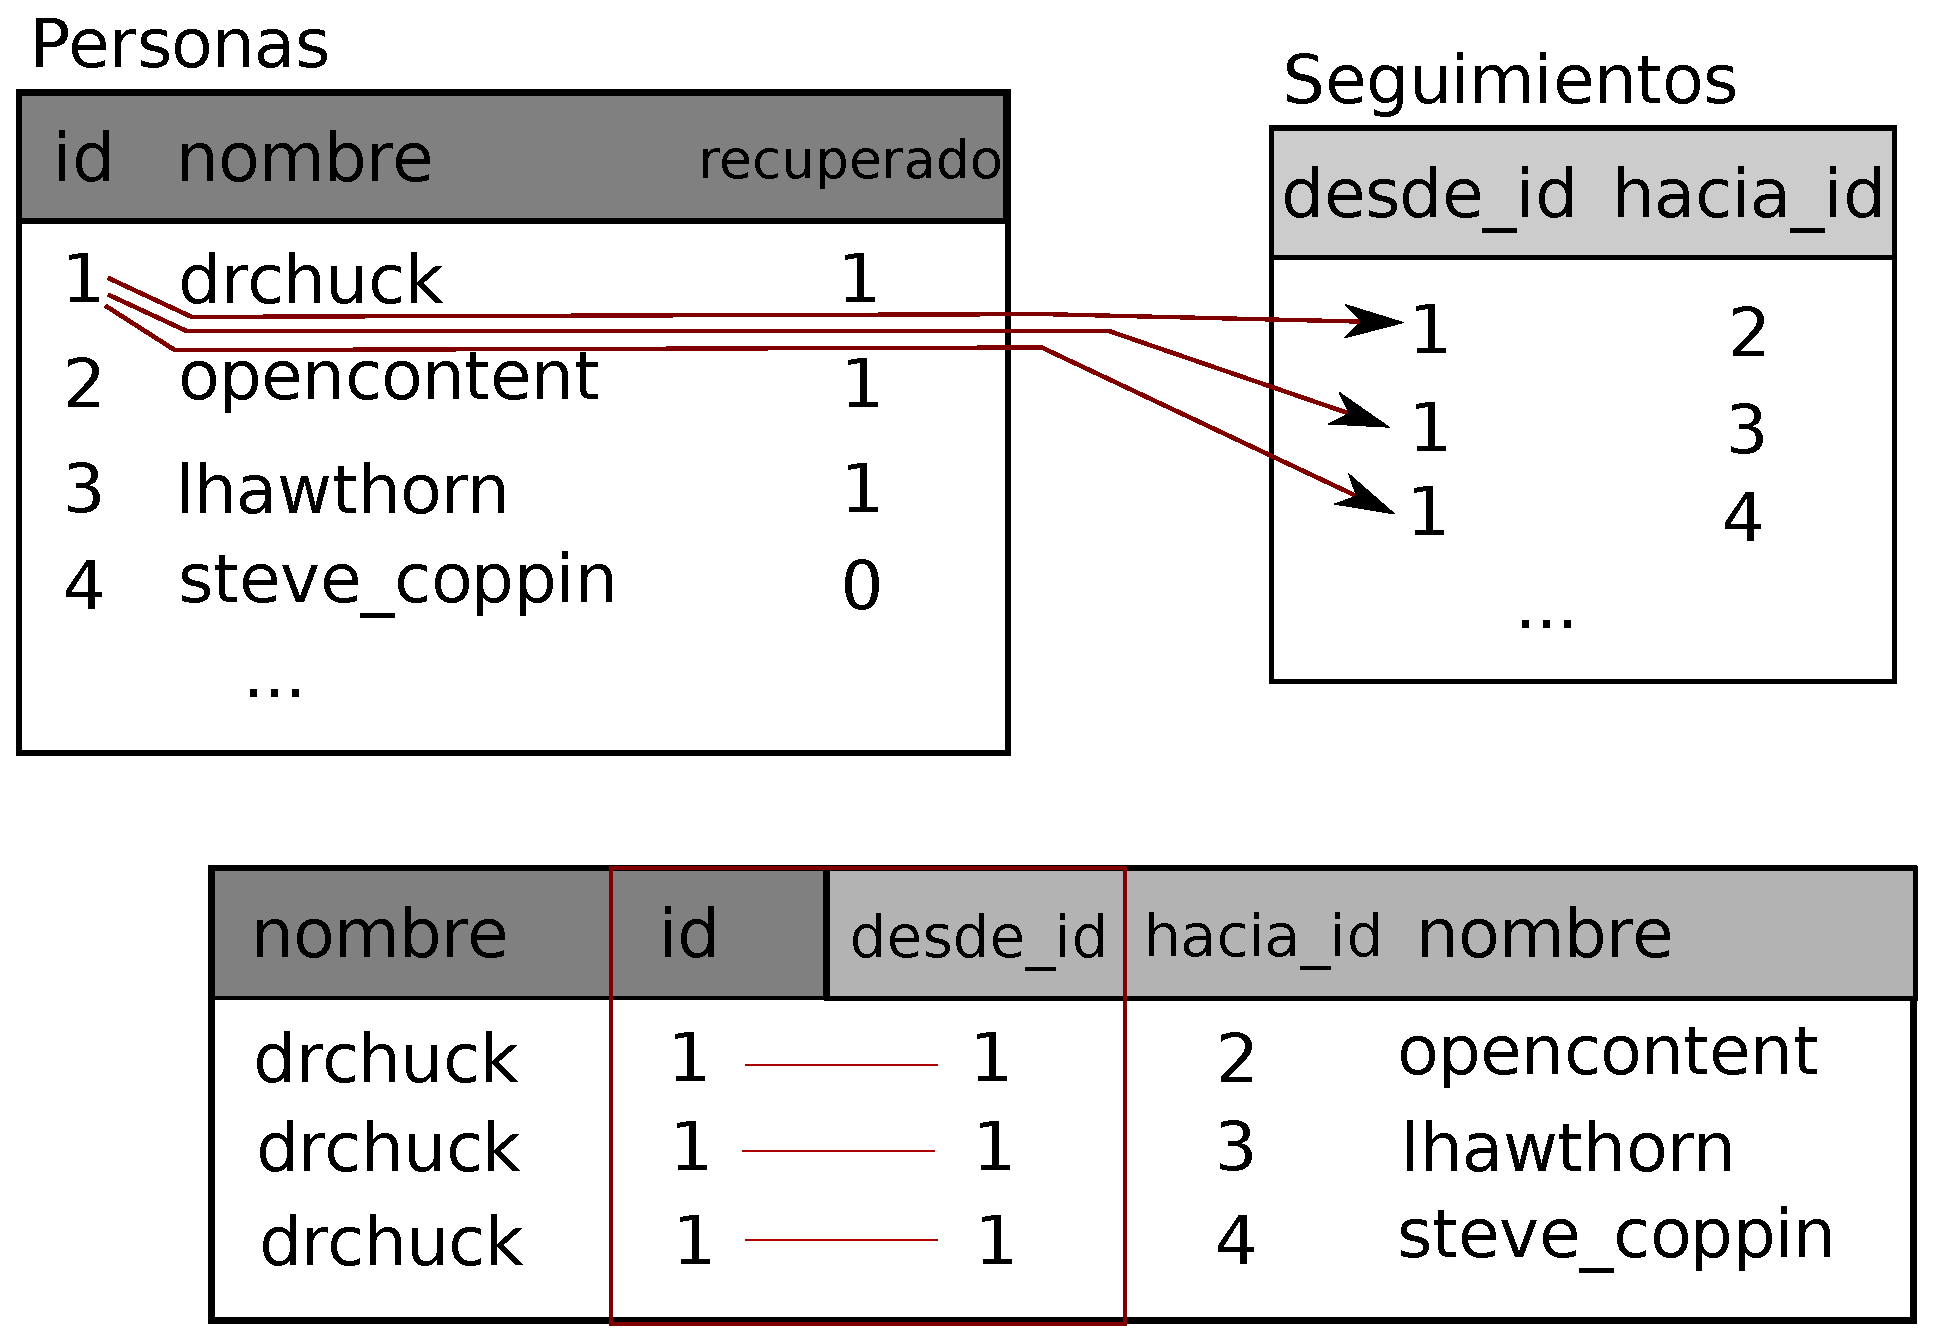
\includegraphics[height=2.50in]{figs2/join.eps}}
\afterfig

El resultado del JOIN consiste en la creación de una ``meta-fila'' extra larga, que contendrá
tanto los campos de {\tt Personas} como los campos de la fila de {\tt Seguimientos} que cumpla la
condición.
Cuando hay más de una coincidencia entre el campo {\tt id} de {\tt Personas}
y el \verb"desde_id" de {\tt Seguimientos}, JOIN creará una meta-fila
para \emph{cada una} de las parejas de filas que coincidan, duplicando los datos si es necesario.

El código siguiente muestra los datos que tendremos en la
base de datos después de que el programa multi-tabla araña de Twitter anterior
haya sido ejecutado varias veces.

\beforeverb
\begin{verbatim}
import sqlite3

conn = sqlite3.connect('arana.sqlite3')
cur = conn.cursor()

cur.execute('SELECT * FROM Personas')
contador = 0
print 'Personas:'
for fila in cur :
   if contador < 5: print fila
   contador = contador + 1
print contador, 'filas.'

cur.execute('SELECT * FROM Seguimientos')
contador = 0
print 'Seguimientos:'
for fila in cur :
   if contador < 5: print fila
   contador = contador + 1
print contador, 'filas.'

cur.execute('''SELECT * FROM Seguimientos JOIN Personas 
    ON Seguimientos.hacia_id = Personas.id WHERE Seguimientos.desde_id = 2''')
contador = 0
print 'Conexiones para id=2:'
for fila in cur :
   if contador < 5: print fila
   contador = contador + 1
print contador, 'filas.'

cur.close()
\end{verbatim}
\afterverb
%
En este programa, en primer lugar volcamos el contenido de las tablas {\tt Personas}
y {\tt Seguimientos} y a continuación mostramos un subconjunto de
datos de las tablas unidas entre sí.

Aquí tenemos la salida del programa:

\beforeverb
\begin{verbatim}
python twjoin.py 
Personas:
(1, u'drchuck', 1)
(2, u'opencontent', 1)
(3, u'lhawthorn', 1)
(4, u'steve_coppin', 0)
(5, u'davidkocher', 0)
55 filas.
Seguimientos:
(1, 2)
(1, 3)
(1, 4)
(1, 5)
(1, 6)
60 filas.
Conexiones para id=2:
(2, 1, 1, u'drchuck', 1)
(2, 28, 28, u'cnxorg', 0)
(2, 30, 30, u'kthanos', 0)
(2, 102, 102, u'SomethingGirl', 0)
(2, 103, 103, u'ja_Pac', 0)
20 filas.
\end{verbatim}
\afterverb
%
Se pueden ver las columnas de las tablas {\tt Personas} y {\tt Seguimientos}, seguidos del último
conjunto de filas, que es el resultado del {\tt SELECT} con la clausula {\tt JOIN}.

En el último select, buscamos las cuentas que sean amigas de
``opencontent'' (es decir, de {\tt Personas.id=2}).

En cada una de las ``meta-filas'' del último select, las primeras dos columnas pertenecen
a la tabla {\tt Seguimientos}, mientras que las columnas tres a cinco pertenecen a la tabla
{\tt Personas}. Se puede observar también cómo la segunda columna (\verb"Seguimientos.hacia_id")
coincide con la tercera ({\tt Personas.id}) en cada una de las ``meta-filas'' del join.

\section{Resumen}

En este capítulo se han tratado un montón de temas para darte una visión de conjunto del uso básico
de las bases de datos en Python. Es más complicado escribir el código para usar una base
de datos que almacene los datos que utilizar diccionarios de Python o archivos planos, de modo que
existen pocas razones para usar una base de datos a menos que tu aplicación necesite de verdad
las capacidades que proporciona. Las situaciones en las cuales una base de datos pueden resultar
bastante útil son:
(1) cuando tu aplicación necesita realizar muchos cambios pequeños de forma aleatoria en un conjunto
de datos grandes,
(2) cuando tienes tantos datos que no caben en un diccionario y necesitas localizar
información con frecuencia, o
(3) cuando tienes un proceso que va a funcionar durante mucho tiempo, y necesitas poder
detenerlo y volverlo a poner en marcha, conservando los datos entre ejecuciones.

Para cubrir las necesidades de muchas aplicaciones, una base de datos con una simple tabla puede
resultar suficiente, pero la mayoría de los problemas necesitarán varias tablas y enlaces/relaciones
entre filas de tablas diferentes. Cuando empieces a crear enlaces entre tablas,
es importante realizar un diseño meditado y seguir las
reglas de normalización de bases de datos para conseguir el mejor uso de sus capacidades.
Como la motivación principal para usar una base de datos
suele ser tener grandes cantidades de datos con las que tratar, resulta importante
modelar los datos de forma eficiente, de modo que tu programa funcione tan rápidamente como sea
posible. 

\section{Depuración}

Un enfoque común cuando se está desarrollando un programa en Python que conecte con
una base de datos SQLite será ejecutar primero el programa y revisar luego los
resultados usando el navegador de bases de datos de SQLite (SQLite Database Browser). El navegador
te permite revisar cuidadosamente los datos para comprobar si tu programa está funcionando
correctamente.

Debes tener cuidado, ya que SQLite se encarga de evitar que dos programa puedan
cambiar los mismos datos a la vez. Por ejemplo, si abres
una base de datos en el navegador y realizas un cambio en la base de datos,
pero no has pulsado aún el botón ``guardar'' del navegador, éste
``bloqueará'' el fichero de la base de datos y evitará que cualquier otro programa
acceda a dicho fichero. Concretamente, en ese caso tu programa Python
no será capaz de acceder al fichero si éste se encuentra bloqueado.

De modo que la solución pasa por asegurarse de cerrar el navegador de la base de datos,
o bien usar el menú {\bf Arhivo} para cerrar la base de datos abierta en el navegador
antes de intentar acceder a ella desde Python, para evitar encontrarse con
el problema de que el código de Python falle debido a que la base de datos
está bloqueada.

\section{Glosario}

\begin{description}

\item[atributo:] Uno de los valores dentro de una tupla. Más comúnmente
llamada ``columna'' o ``campo''..
\index{atributo}

\item[cursor:] Un cursor permite ejecutar comandos SQL en una base de datos
y recuperar los datos de ella. Un cursor es similar a un
socket en conexiones de red o a un manejador de ficheros.
\index{cursor}

\item[clave foránea:] Una clave numérica que apunta a la clave primaria de
una fila en otra tabla. Las claves foráneas establecen relaciones entre filas
almacenadas en tablas diferentes.
\index{foránea, clave}
\index{clave!foránea}

\item[clave lógica:] Una clave que el ``mundo exterior'' utiliza para localizar una fila
concreta. Por ejemplo, en una tabla de cuentas de usuario, la dirección de e-mail de una persona
sería un buen candidato a utilizar como clave lógica para los datos de ese usuario.
\index{lógica, clave}
\index{clave!lógica}

\item[clave primaria:] Una clave numérica asignada a cada fila que es utilizada para
referirnos a esa fila concreta de esa tabla desde otra tabla distinta. A menudo la base de datos
se configura para asignar las claves primarias de forma automática, según se van insertando filas.
\index{primaria, clave}
\index{clave!primaria}

\item[índice:] Datos adicionales que el software de la base de datos mantiene como filas
e inserta en una tabla para conseguir que las búsquedas sean muy rápidas.
\index{índice}

\item[navegador de base de datos:]
Un programa que permite conectar directamente con una base de datos
y manipularla, sin tener que escribir código para ello.
\index{gestor de bases de datos}
\index{base de datos!gestor}

\item[normalización:] Diseño de un modelado de datos de forma que no haya datos
duplicados. Se almacena cada elemento de los datos en un lugar concreto de la base de datos
y se referencia desde otros sitios usando una clave foránea.
\index{normalización}
\index{base de datos!normalización}

\item[relación:] Un área dentro de una base de datos que contiene tuplas y
atributos. Se la conoce más habitualmente como ``tabla''.
\index{relación}

\item[restricción:]
Cuando le pedimos a una base de datos que imponga una regla a una campo de una fila
en una tabla. Una restricción habitual consiste en especificar que no pueda haber
valores repetidos en un campo concreto (es decir, que todos los valores deban ser únicos). 
\index{restricción}

\item[tupla:] Una entrada única en una base de datos, que es un conjunto
de atributos. Se la conoce más habitualmente como ``fila''.
\index{tupla}

\end{description}
% The contents of this file is 
% Copyright (c) 2009-  Charles R. Severance, All Righs Reserved

\chapter{Visualizando datos}

Hasta ahora, primero hemos estudiado el lenguaje de Python y luego
hemos descubierto cómo usar Python, la red y las bases de datos
para manipular datos.

En este capítulo, echaremos un vistazo a tres
aplicaciones completas que reúnen todas esas cosas
para gestionar y visualizar datos. Puedes usar estas aplicaciones
como código de ejemplo que te puede servir de punto de partida para la
resolución de problemas del mundo real.

Cada una de las aplicaciones es un archivo ZIP que puedes descargar,
extraer en tu ordenador y ejecutar.

\section{Construcción de un mapa de Google a partir de datos geocodificados}
\index{Google!map}
\index{Visualization!map}

En este proyecto usaremos la API de geocodificación de Google
para limpiar varias ubicaciones geográficas de nombres de universidades
introducidas por los usuarios, y luego colocaremos los datos en
un mapa de Google. 

\beforefig
\centerline{\includegraphics[height=2.25in]{figs2/google-map.eps}}
\afterfig

Para comenzar, descarga la aplicación desde:

\url{www.py4inf.com/code/geodata.zip}

El primer problema a resolver es que la API libre de geocodificación
de Google tiene como límite de uso un cierto número de peticiones diarias. Si tienes
un montón de datos, necesitarás detener y reanudar el proceso de
búsqueda varias veces. De modo que dividiremos el problema en
dos fases.

\index{cache}
En la primera fase, tomaremos como entrada los datos ``de reconocimiento'' del archivo
{\bf where.data} y los leeremos línea a línea, recuperando la
información de geocodificación desde Google y almacenándola
en una base de datos {\bf geodata.sqlite}.
Antes de usar la API de geocodificación para cada ubicación introducida por los usuarios,
verificaremos si ya tenemos los datos para esa entrada
concreta. La base de datos funcionará así como una ``caché'' local
de datos de geocodificación, para asegurarnos de que nunca solicitamos
a Google los mismos datos dos veces.

Puedes reiniciar el proceso en cualquier momento eliminando el archivo
{\bf geodata.sqlite}.

Ejecuta el programa {\bf geoload.py}. Este programa leerá las líneas
de entrada desde {\bf where.data} y para cada línea verificará primero si ya
está en la base de datos. Si no disponemos de datos para esa ubicación,
llamará a la API de geocodificación para recuperar los datos y los almacenará
en la base de datos.

Aquí tenemos un ejemplo de ejecución una vez que ya disponemos de alguna información almacenada en la
base de datos:

\beforeverb
\begin{verbatim}
Found in database  Northeastern University
Found in database  University of Hong Kong, ...
Found in database  Technion
Found in database  Viswakarma Institute, Pune, India
Found in database  UMD
Found in database  Tufts University

Resolving Monash University
Retrieving http://maps.googleapis.com/maps/api/
    geocode/json?sensor=false&address=Monash+University
Retrieved 2063 characters {    "results" : [  
{u'status': u'OK', u'results': ... }

Resolving Kokshetau Institute of Economics and Management
Retrieving http://maps.googleapis.com/maps/api/
    geocode/json?sensor=false&address=Kokshetau+Inst ...
Retrieved 1749 characters {    "results" : [  
{u'status': u'OK', u'results': ... }
...
\end{verbatim}
\afterverb
%
Las primeras cinco ubicaciones ya están en la base de datos y por eso
las omitimos. El programa explora hasta que encuentra ubicaciones
nuevas y entonces comienza a recuperarlas.

El programa {\bf geoload.py} puede ser detenido en cualquier momento, y dispone de un
contador que puedes usar para limitar el número de llamadas a la API de geolocalización
en cada ejecución. Dado que el fichero {\bf where.data} sólo tiene unos pocos cientos
de elementos, no deberías llegar al límite diario de usos, pero si
tienes más datos pueden ser necesarias varias ejecuciones del programa durante varios días
para conseguir tener todos los datos de entrada geolocalizados en nuestra base de datos.

Una vez que tienes parte de los datos cargados en {\bf geodata.sqlite}, se pueden
visualizar usando el programa {\bf geodump.py}. Este
programa lee la base de datos y escribe el arhivo {\bf where.js}
con la ubicación, latitud y longitud en forma de
código ejecutable JavaScript.

Una ejecución del programa {\bf geodump.py} sería la siguiente: 

\beforeverb
\begin{verbatim}
Northeastern University, ... Boston, MA 02115, USA 42.3396998 -71.08975
Bradley University, 1501 ... Peoria, IL 61625, USA 40.6963857 -89.6160811
...
Technion, Viazman 87, Kesalsaba, 32000, Israel 32.7775 35.0216667
Monash University Clayton ... VIC 3800, Australia -37.9152113 145.134682
Kokshetau, Kazakhstan 53.2833333 69.3833333
...
12 records written to where.js
Open where.html to view the data in a browser
\end{verbatim}
\afterverb
%
El archivo {\bf where.html} consiste en HTML y JavaScript para mostrar
un mapa de Google. Lee los datos más actuales de {\bf where.js} para obtener
los datos que se visualizarán. He aquí el formato del fichero {\bf where.js}:

\beforeverb
\begin{verbatim}
myData = [
[42.3396998,-71.08975, 'Northeastern Uni ... Boston, MA 02115'],
[40.6963857,-89.6160811, 'Bradley University, ... Peoria, IL 61625, USA'],
[32.7775,35.0216667, 'Technion, Viazman 87, Kesalsaba, 32000, Israel'],
   ...
];
\end{verbatim}
\afterverb
%
Se trata de una variable JavaScript que contiene una lista de listas.
La sintaxis de las listas de constantes en JavaScript es muy similar a
las de Python, de modo que la sintaxis debería resultarte familiar.

Simplemente abre {\bf where.html} en un navegador para ver las ubicaciones.
Puedes mantener el ratón sobre cada marca del mapa para ver la
ubicación que la API de geocodificación ha devuelto para la entrada que el usuario introdujo.
Si no puedes ver ningún dato cuando abras el fichero {\bf where.html}, deberás
verificar que tengas activado JavaScript o usar la consola de desarrollador de tu navegador.

\section{Visualización de redes e interconexiones}
\index{Google!page rank}
\index{Visualization!networks}
\index{Visualization!page rank}

En la siguiente aplicación, realizaremos algunas de las funciones de un motor
de búsqueda. Primero rastrearemos una pequeña parte de la web y ejecutaremos
una versión simplificada del algoritmo de clasificación que usa la página de Google
para determinar qué páginas son las más visitadas. Luego visualizaremos
la clasificación de las páginas y visitas de nuestro pequeño rincón de la web.
Usaremos la librería de visualización de JavaScript D3
\url{http://d3js.org/} para generar la imagen de salida.

Puedes descargar y extraer esta aplicación desde:

\url{www.py4inf.com/code/pagerank.zip}

\beforefig
\centerline{\includegraphics[height=2.25in]{figs2/pagerank.eps}}
\afterfig

El primer programa ({\bf spider.py}) rastrea un sitio web
y envía una serie de páginas a la
base de datos ({\bf spider.sqlite}), guardando los enlaces entre páginas.
Puedes reiniciar el proceso en cualquier momento eliminando el
fichero {\bf spider.sqlite} y ejecutando de nuevo {\bf spider.py}.

\beforeverb
\begin{verbatim}
Enter web url or enter: http://www.dr-chuck.com/
['http://www.dr-chuck.com']
How many pages:2
1 http://www.dr-chuck.com/ 12
2 http://www.dr-chuck.com/csev-blog/ 57
How many pages:
\end{verbatim}
\afterverb
%
En esta ejecución de ejemplo, le pedimos que rastree un sitio web y que recupere dos
páginas. Si reinicias el programa y le pides que rastree más
páginas, no volverá a revisar aquellas que ya estén en la base de datos.
En cada reinicio irá a una página al azar no rastreada aún y comenzará allí.
De modo que cada ejecución sucesiva de {\bf spider.py} irá añadiendo páginas nuevas.

\beforeverb
\begin{verbatim}
Enter web url or enter: http://www.dr-chuck.com/
['http://www.dr-chuck.com']
How many pages:3
3 http://www.dr-chuck.com/csev-blog 57
4 http://www.dr-chuck.com/dr-chuck/resume/speaking.htm 1
5 http://www.dr-chuck.com/dr-chuck/resume/index.htm 13
How many pages:
\end{verbatim}
\afterverb
%
Se pueden tener múltiples puntos de partida en la misma base de datos---dentro
del programa, estos son llamados ``webs''. La araña
elije entre todos los enlaces no visitados de las páginas existentes uno al azar
como siguiente página a rastrear.

Si quieres ver el contenido del fichero {\bf spider.sqlite}, puedes
ejecutar {\bf spdump.py}, que mostrará algo como esto:

\beforeverb
\begin{verbatim}
(5, None, 1.0, 3, u'http://www.dr-chuck.com/csev-blog')
(3, None, 1.0, 4, u'http://www.dr-chuck.com/dr-chuck/resume/speaking.htm')
(1, None, 1.0, 2, u'http://www.dr-chuck.com/csev-blog/')
(1, None, 1.0, 5, u'http://www.dr-chuck.com/dr-chuck/resume/index.htm')
4 rows.
\end{verbatim}
\afterverb
%
Se muestra el número de enlaces hacia la página, la clasificación antigua de la página, la
clasificación nueva, el id de la página, y la url de la página. El programa {\bf spdump.py}
sólo muestra aquellas páginas que tienen al menos un enlace hacia ella.

Una vez que tienes unas cuantas páginas en la base de datos, puedes ejecutar el clasificador sobre ellas, usando el programa {\bf sprank.py}. Simplemente debes indicarle cuántas
iteraciones del clasificador de páginas debe realizar.

\beforeverb
\begin{verbatim}
How many iterations:2
1 0.546848992536
2 0.226714939664
[(1, 0.559), (2, 0.659), (3, 0.985), (4, 2.135), (5, 0.659)]
\end{verbatim}
\afterverb
%
Puedes volcar en pantalla el contenido la base de datos de nuevo para ver que la clasificación de
páginas ha sido actualizada:

\beforeverb
\begin{verbatim}
(5, 1.0, 0.985, 3, u'http://www.dr-chuck.com/csev-blog')
(3, 1.0, 2.135, 4, u'http://www.dr-chuck.com/dr-chuck/resume/speaking.htm')
(1, 1.0, 0.659, 2, u'http://www.dr-chuck.com/csev-blog/')
(1, 1.0, 0.659, 5, u'http://www.dr-chuck.com/dr-chuck/resume/index.htm')
4 rows.
\end{verbatim}
\afterverb
%
Puedes ejecutar {\bf sprank.py} tantas veces com quieras, y simplemente irá refinando
la clasificación de páginas cada vez más. Puedes incluso ejecutar {\bf sprank.py} varias veces,
luego ir a la araña {\bf spider.py} a recuperar unas cuantas páginas más y después ejecutar de nuevo
{\bf sprank.py} para actualizar los valores de clasificación. Un motor de búsqueda normalmente
ejecuta ambos programas (el rastreador y el clasificador) de forma constante.

Si quieres reiniciar los cálculos de clasificación de páginas sin tener que rastrear de nuevo
las páginas web, puedes usar {\bf spreset.py} y después reiniciar {\bf sprank.py}.

\beforeverb
\begin{verbatim}
How many iterations:50
1 0.546848992536
2 0.226714939664
3 0.0659516187242
4 0.0244199333
5 0.0102096489546
6 0.00610244329379
...
42 0.000109076928206
43 9.91987599002e-05
44 9.02151706798e-05
45 8.20451504471e-05
46 7.46150183837e-05
47 6.7857770908e-05
48 6.17124694224e-05
49 5.61236959327e-05
50 5.10410499467e-05
[(512, 0.0296), (1, 12.79), (2, 28.93), (3, 6.808), (4, 13.46)]
\end{verbatim}
\afterverb
%
En cada iteración del algoritmo de clasificación de páginas se muestra el cambio
medio en la clasificación de cada página. La red al principio está bastante
desequilibrada, de modo que los valores de esos cambios medios de clasificación
para cada página variarán a lo loco entre iteraciones. Pero después de unas cuantas
iteraciones, la clasificación de páginas converge. Deberías
ejecutar {\bf prank.py} durante el tiempo suficiente para que los valores de clasificación
converjan.

Si quieres visualizar las páginas mejor clasificadas hasta ese momento,
ejecuta {\bf spjson.py} para leer desde base de datos y escribir el ranking de
las páginas más enlazadas en formato JSON, que puede ser visualizado en
un navegador web.

\beforeverb
\begin{verbatim}
Creating JSON output on spider.json...
How many nodes? 30
Open force.html in a browser to view the visualization
\end{verbatim}
\afterverb
%
Puedes ver esos datos abriendo el fichero {\bf force.html} en tu navegador.
Mostrará un diseño automático de los nodos y enlaces. Puedes pinchar y
arrastrar cualquier nodo y también hacer doble click sobre él para ver la URL
que representa.

Si vuelves a ejecutar las otras utilidades, ejecuta {\bf spjson.py} y
pulsar ``recargar'' en el navegador para obtener los datos actualizados desde {\bf spider.json}.

\section{Visualización de datos de correo}

Si has llegado hasta este punto del libro, ya debes estar bastante familiarizado con
nuestros ficheros de datos {\bf mbox-short.txt} y {\bf mbox.txt}. Ahora es el momento
de llevar nuestro análisis de datos de correo electrónico al siguiente nivel.

En el mundo real, a veces se tienen que descargar datos de correo desde los servidores.
Eso podría llevar bastante tiempo y los datos podrían tener inconsistencias,
estar llenos de errores, y necesitar un montón de limpieza y ajustes. En esta sección,
trabajaremos con la aplicación más compleja que hemos visto hasta ahora, que
descarga casi un gigabyte de datos y los visualiza.

\beforefig
\centerline{\includegraphics[height=2.50in]{figs2/wordcloud.eps}}
\afterfig

Puedes descargar la aplicación desde:

\url{www.py4inf.com/code/gmane.zip}

Utilizaremos los datos de un servicio de archivo de listas de correo electrónico libre,
llamado \url{www.gmane.org}. Este servicio es muy popular en proyectos de código abierto,
debido a que proporciona un buen almacenaje con capacidad de búsqueda de su
actividad de correo. También tienen una política muy liberal respecto al acceso a
sus datos a través de su API. No tienen límites de acceso, pero te piden que no
sobrecargues su servicio y descargues sólo los datos que necesites. Puedes leer
los términos y condiciones de gmane en su página:

\url{http://gmane.org/export.php}

{\em Es muy importante que hagas uso de los datos de gname.org con
responsabilidad, añadiendo retrasos en tus accesos a sus servicios y extendiendo
la realización de los procesos de larga duración a periodos de tiempo lo suficientemente largos.
No abuses de este servicio libre y lo estropees para los demás.}

Cuando se usa este software para rastrear los datos de correo de Sakai, se genera casi
un Gigabyte de datos y se necesita una cantidad considerable de ejecuciones durante varios días.
El archivo {\bf README.txt} del ZIP anterior contiene instrucciones sobre cómo
descargar una copia pre-rastreada del fichero {\bf content.sqlite} con
la mayor parte del contenido de los correos de Sakai, de modo que no tengas que rastrear
durante cinco días sólo para hacer funcionar los programas. Aunque descargues el contenido
pre-rastreado, deberías ejecutar el proceso de rastreo para recuperar los
mensajes más recientes.

El primer paso es rastrear el repositorio gmane. La URL base
se puede modificar en {\bf gmane.py}, y por defecto apunta a la lista
de desarrolladores de Sakai. Puedes rastrear otro repositorio cambiando la
url base. Asegúrate de borrar el fichero {\bf content.sqlite} si realizas
el cambio de url.

El fichero {\bf gmane.py} opera como una araña caché responsable, que
funciona despacio y recupera un mensaje de correo por segundo para
evitar ser bloqueado por gmane. Almacena todos sus datos
en una base de datos y puede ser interrumpido y reanudado tantas veces como
sean necesarias. Puede llevar muchas horas descargar todos los datos.
De modo que tendrás que reanudarlo varias veces.

He aquí una ejecución de {\bf gmane.py} recuperando los últimos cinco mensajes de
la lista de desarrolladores de Sakai:

\beforeverb
\begin{verbatim}
How many messages:10
http://download.gmane.org/gmane.comp.cms.sakai.devel/51410/51411 9460
    nealcaidin@sakaifoundation.org 2013-04-05 re: [building ...
http://download.gmane.org/gmane.comp.cms.sakai.devel/51411/51412 3379
    samuelgutierrezjimenez@gmail.com 2013-04-06 re: [building ...
http://download.gmane.org/gmane.comp.cms.sakai.devel/51412/51413 9903
    da1@vt.edu 2013-04-05 [building sakai] melete 2.9 oracle ...
http://download.gmane.org/gmane.comp.cms.sakai.devel/51413/51414 349265
    m.shedid@elraed-it.com 2013-04-07 [building sakai] ...
http://download.gmane.org/gmane.comp.cms.sakai.devel/51414/51415 3481
    samuelgutierrezjimenez@gmail.com 2013-04-07 re: ...
http://download.gmane.org/gmane.comp.cms.sakai.devel/51415/51416 0

Does not start with From 
\end{verbatim}
\afterverb
%
El programa revisa {\bf content.sqlite} desde el principio hasta que encuentra un número de mensaje que
no ha sido aún rastreado y comienza a partir de ahí. Continúa rastreando
hasta que ha recuperado el número deseado de mensajes o hasta que llega a una página
que no contiene un mensaje adecuadamente formateado.

A veces \url{gmane.org} pierde un mensaje. Tal vez los administradores lo borraron,
o quizás simplemente se perdió. Si tu araña se detiene, y parece que ha localizado
un mensaje perdido, entra en el SQLite Manager, añade una fila con el id perdido y los
demás campos en blanco y reanuda {\bf gmane.py}. Así se desbloqueará el
proceso de rastreo y podrá continuar. Esos mensajes vacíos serán ignorados en la siguiente
fase del proceso.

Algo bueno es que una vez que has rastreado todos los mensajes y los tienes en
{\bf content.sqlite}, puedes ejecutar {\bf gmane.py} otra vez para obtener los mensajes
nuevos según van siendo enviados a la lista.

Los datos en {\bf content.sqlite} están guardados en bruto, con un modelado de datos
ineficiente y sin comprimir.
Esto se ha hecho así intencionadamente, para permitirte echar un vistazo en {\bf content.sqlite}
usando el SQLite Manager y depurar problemas con el proceso de rastreo.
Sería una mala idea ejecutar cualquier consulta sobre esta base de datos, ya que
puede resultar bastante lenta.

El segundo proceso consiste en ejecutar el programa {\bf gmodel.py}. Este programa lee los datos
en bruto de {\bf content.sqlite} y produce una versión limpia y bien modelada de los datos,
que envía al fichero {\bf index.sqlite}. Este fichero es mucho más pequeño (puede ser 10 veces
menor) que {\bf content.sqlite}, porque también comprime la cabecera y el texto del cuerpo.

Cada vez que {\bf gmodel.py} se ejecuta, borra y reconstruye {\bf index.sqlite}, permitiéndote
ajustar sus parámetros y editar las tablas de mapeo de {\bf content.sqlite} para ajustar el
proceso de limpieza de datos. Esto es un ejemplo de ejecución de {\bf gmodel.py}. El programa imprime
una línea en pantalla cada vez que son procesados 250 mensajes de correo para que puedas ver su
evolución, ya que puede quedarse funcionando durante un buen rato mientras procesa alrededor de
un Gigabyte de datos de correo.

\beforeverb
\begin{verbatim}
Loaded allsenders 1588 and mapping 28 dns mapping 1
1 2005-12-08T23:34:30-06:00 ggolden22@mac.com
251 2005-12-22T10:03:20-08:00 tpamsler@ucdavis.edu
501 2006-01-12T11:17:34-05:00 lance@indiana.edu
751 2006-01-24T11:13:28-08:00 vrajgopalan@ucmerced.edu
...
\end{verbatim}
\afterverb
%
El programa {\bf gmodel.py} realiza varias labores de limpieza de datos.

Los nombres de dominio son truncados a dos niveles para .com, .org, .edu y .net.
Otros nombres de dominio son truncados a tres niveles. De modo que si.umich.edu se transforma en
umich.edu, y caret.cam.ac.uk queda como cam.ac.uk. Las direcciones de correo electrónico también
son transformadas a minúsculas, y algunas de las direcciones de @gmane.org, como las siguientes

\beforeverb
\begin{verbatim}
   arwhyte-63aXycvo3TyHXe+LvDLADg@public.gmane.org
\end{verbatim}
\afterverb
%
son convertidas en direcciones reales, cuando esa dirección de correo real existe
en otra parte del cuerpo del mensaje.

En la base de datos {\bf content.sqlite} existen dos tablas que te permiten
mapear tanto nombres de dominios como direcciones de correo individuales que van cambiando
a lo largo del tiempo de existencia de la lista de correo. Por ejemplo, Steve Githens ha usado las
direcciones de correo siguientes, según iba cambiando de trabajo a lo largo del tiempo de existencia
de la lista de desarrolladores de Sakai:

\beforeverb
\begin{verbatim}
s-githens@northwestern.edu
sgithens@cam.ac.uk
swgithen@mtu.edu
\end{verbatim}
\afterverb
%
Podemos añadir dos entradas en la tabla de Mapeo (Mapping) de {\bf content.sqlite}, de modo
que {\bf gmodel.py} mapeará las tres direcciones en una:

\beforeverb
\begin{verbatim}
s-githens@northwestern.edu ->  swgithen@mtu.edu
sgithens@cam.ac.uk -> swgithen@mtu.edu
\end{verbatim}
\afterverb
%
Puedes crear entradas similares en la tabla DNSMapping si hay múltiples nombres
DNS que quieres mapear a una única DNS. El mapeo siguiente ha sido añadido a los datos de Sakai:

\beforeverb
\begin{verbatim}
iupui.edu -> indiana.edu
\end{verbatim}
\afterverb
%
de modo que todas las cuentas de los distintos campus de las Universidades de Indiana son
rastreados juntos.

Puedes volver a ejecutar {\bf gmodel.py} una y otra vez mientras vas mirando los datos, y añadir
mapeos para hacer que los datos queden más y más limpios. Cuando lo hayas hecho, tendrás una bonita
versión indexada del correo en {\bf index.sqlite}. Éste es el fichero que usaremos para realizar
el análisis de datos. Con ese fichero, el análisis de datos se realizará muy rápidamente.

El primer y más sencillo análisis de datos consistirá en determinar ``¿quién ha enviado más correos?'',
y ´´¿qué organización ha enviado más correos?''. Esto se realizará usando {\bf gbasic.py}:

\beforeverb
\begin{verbatim}
How many to dump? 5
Loaded messages= 51330 subjects= 25033 senders= 1584

Top 5 Email list participants
steve.swinsburg@gmail.com 2657
azeckoski@unicon.net 1742
ieb@tfd.co.uk 1591
csev@umich.edu 1304
david.horwitz@uct.ac.za 1184

Top 5 Email list organizations
gmail.com 7339
umich.edu 6243
uct.ac.za 2451
indiana.edu 2258
unicon.net 2055
\end{verbatim}
\afterverb
%
Fijate cómo {\bf gbasic.py} funciona mucho más rápido que {\bf gmane.py},
e incluso que {\bf gmodel.py}. Todos trabajan con los mismos datos, pero
{\bf gbasic.py} está usando los datos comprimidos y normalizados de
{\bf index.sqlite}. Si tienes un montón de datos que gestionar, un proceso
multipaso como el que se realiza en esta aplicación puede ser más largo de desarrollar,
pero te ahorrará un montón de tiempo cuando realmente comiences a explorar
y visualizar los datos.

Puedes generar una vista sencilla con la frecuencia de cada palabras en las
líneas de título, usando el archivo {\bf gword.py}:

\beforeverb
\begin{verbatim}
Range of counts: 33229 129
Output written to gword.js
\end{verbatim}
\afterverb
%
Esto genera el archivo {\bf gword.js}, que puedes visualizar utilizando
{\bf gword.htm} para producir una nube de palabras similar a la del comienzo
de esta sección. 

{\bf gline.py} produce una segunda vista. En este caso cuenta la participación
en forma de correos de las organizaciones a lo largo del tiempo.

\beforeverb
\begin{verbatim}
Loaded messages= 51330 subjects= 25033 senders= 1584
Top 10 Oranizations
['gmail.com', 'umich.edu', 'uct.ac.za', 'indiana.edu', 
'unicon.net', 'tfd.co.uk', 'berkeley.edu', 'longsight.com', 
'stanford.edu', 'ox.ac.uk']
Output written to gline.js
\end{verbatim}
\afterverb
%
Su salida es guardada en {\bf gline.js}, que se puede visualizar usando {\bf gline.htm}.

\beforefig
\centerline{\includegraphics[height=2.50in]{figs2/mailorg.eps}}
\afterfig

Esta aplicación es relativamente compleja y sofisticada, y
dispone de características para realizar recuperación de datos reales, limpieza y visualización.

% The contents of this file is 
% Copyright (c) 2009-  Charles R. Severance, All Righs Reserved

\chapter{Automatización de tareas habituales en tu ordenador}

Hemos estado leyendo datos desde ficheros, redes, servicios y
bases de datos. Python puede moverse también a través de todos los
directorios y carpetas de tus equipos y además leer
los ficheros.

En este capítulo, vamos a escribir programas que busquen
por todo el ordenador y
realicen ciertas operaciones sobre cada fichero.
Los archivos están organizados en directorios (también llamados ``carpetas'').
Scripts sencillos en Python
pueden ocuparse de tareas simples que se tengan que repetir
sobre cientos o miles de ficheros
distribuidos a lo largo de un arbol de directorios o incluso por todo el ordenador.

Para movernos a través de todos los directorios y archivos de un árbol usaremos
{\tt os.walk} y un bucle {\tt for}. Es similar a cómo
{\tt open} nos permite usar un bucle para leer el contenido de un archivo,
{\tt socket} nos permite usar un bucle para leer el contenido de una conexión de red, y
{\tt urllib} nos permite abrir un documento web y movernos a través de su contenido. 

\section{Nombres de archivo y rutas}
\label{paths}

\index{archivo, nombre}
\index{ruta}
\index{directorio}
\index{carpeta}

Cada programa en ejecución tiene su propio ``directorio actual'', que es el directorio que
usará por defecto para la mayoría de las operaciones. Por ejemplo, cuando abres un archivo
en modo lectura, Python lo busca en el directorio actual.

\index{os, módulo}
\index{módulo!os}

El módulo {\tt os} proporciona funciones para trabajar con archivos y
directorios ({\tt os} significa ``Sistema Operativo''\footnote{en inglés, ``operating system''
(Nota del trad.)}).
{\tt os.getcwd} devuelve el nombre del directorio actual:

\index{getcwd, función}
\index{función!getcwd}

\beforeverb
\begin{verbatim}
>>> import os
>>> cwd = os.getcwd()
>>> print cwd
/Users/csev
\end{verbatim}
\afterverb
%
{\tt cwd} significa {\bf directorio de trabajo actual}\footnote{en inglés, ``current working
directory'' (Nota del trad.)}. El resultado en
este ejemplo es {\tt /Users/csev}, que es el directorio home para un
usuario llamado {\tt csev}.

\index{trabajo, directorio de}
\index{directorio!de trabajo}

Una cadena como {\tt cwd}, que identifica un fichero, recibe el nombre de ruta.
Una {\bf ruta relativa} comienza en el directorio actual;
una {\bf ruta absoluta} comienza en el directorio superior del
sistema de archivos.

\index{relativa, ruta}
\index{ruta!relativa}
\index{absoluta, ruta}
\index{ruta!absoluta}

Las rutas que hemos visto hasta ahora son simples nombres de archivo, de modo que
son relativas al directorio actual. Para encontrar la ruta absoluta de
un archivo se puede utilizar {\tt os.path.abspath}:

\beforeverb
\begin{verbatim}
>>> os.path.abspath('memo.txt')
'/Users/csev/memo.txt'
\end{verbatim}
\afterverb
%
{\tt os.path.exists} comprueba
si un fichero o directorio existe:

\index{exists, función}
\index{función!exists}

\beforeverb
\begin{verbatim}
>>> os.path.exists('memo.txt')
True
\end{verbatim}
\afterverb
%
Si existe, {\tt os.path.isdir} comprueba si se trata de un directorio:

\beforeverb
\begin{verbatim}
>>> os.path.isdir('memo.txt')
False
>>> os.path.isdir('musica')
True
\end{verbatim}
\afterverb
%
De forma similar, {\tt os.path.isfile} comprueba si se trata de un fichero.

{\tt os.listdir} devuelve una lista de los archivos (y otros directorios)
existentes en el directorio dado:

\beforeverb
\begin{verbatim}
>>> os.listdir(cwd)
['musica', 'fotos', 'memo.txt']
\end{verbatim}
\afterverb
%


\section{Ejemplo: Limpieza de un directorio de fotos}

Hace algún tiempo, construí un software parecido a Flickr, que
recibía fotos desde mi teléfono móvil y las almacenaba
en mi servidor. Lo escribí antes de que Flickr existiera y he continuado
usándolo después, porque quería mantener las copias originales
de mis imágenes para siempre.

También quería enviar una descripción sencilla, con una línea de texto en el mensaje MMS,
en la línea de título del correo. Almacené esos mensajes
en un fichero de texto en el mismo directorio que el fichero con la imagen.
Se me ocurrió una estructura de directorios basada en el mes, año, día y hora en
que cada foto había sido realizada. Lo siguiente sería un ejemplo del nombre
de una foto y su descripción:

\beforeverb
\begin{verbatim}
./2006/03/24-03-06_2018002.jpg
./2006/03/24-03-06_2018002.txt
\end{verbatim}
\afterverb
%
Después de siete años, tenía un montón de fotos y descripciones. A lo largo de los años,
según iba cambiando de teléfono móvil, a veces mi código para extraer el texto de los mensajes
fallaba y añadía un montón de datos inútiles al servidor en lugar de la descripción.

Quería moverme a través de esos ficheros y averiguar cuáles de los
textos eran realmente descripciones y cuales eran basura, para poder eliminar
los ficheros erróneos. Lo primero que hice fue generar un sencillo inventario de
cuántos archivos de texto tenía en uno de los subdirectorios,
usando el programa siguiente:

\beforeverb
\begin{verbatim}
import os
contador = 0
for (nombredir, dirs, ficheros) in os.walk('.'):
   for nombrefichero in ficheros:
       if nombrefichero.endswith('.txt') :
           contador = contador + 1
print 'Ficheros:', contador

python txtcount.py
Ficheros: 1917
\end{verbatim}
\afterverb
%
El trozo de código que hace eso posible es la librería de Python
{\tt os.walk}. Cuando llamamos a {\tt os.walk} y le damos un directorio
de inicio, ``recorrerá''\footnote{``walk'' significa ``recorrer'' (Nota del trad.)}
todos los directorios y subdirectorios de forma recursiva. La cadena ``.'' le indica
que comience en el directorio actual y se mueva hacia delante.
A medida que va encontrando directorios, obtenemos tres valores en una tupla
en el cuerpo del bucle {\tt for}. El primer valor es el nombre del
directorio actual, el segundo es la lista de subdirectorios dentro
del actual y el tercer valor es la lista de ficheros
que se encuentran en ese directorio.

No necesitamos mirar explícitamente dentro de cada uno de los subdirectorios,
porque podemos contar con que {\tt os.walk} terminará visitando cada
uno de ellos. Pero sí que tendremos que fijarnos en cada fichero, de
modo que usamos un sencillo bucle {\tt for} para examinar cada uno de los archivos
en el directorio actual. Verificamos cada fichero para comprobar si
termina por ``.txt'', y luego contamos el número de
ficheros en todo el árbol de directorios que terminan con ese
sufijo.

Una vez que tenemos una noción acerca de cuántos archivos terminan por ``.txt'', lo
siguiente es intentar determinar automáticamente
desde Python qué ficheros son incorrectos y cuáles están bien.
De modo que escribiremos un programa sencillo para imprimir en pantalla los
nombres de los ficheros y el tamaño de cada uno:

\beforeverb
\begin{verbatim}
import os
from os.path import join
for (nombredir, dirs, ficheros) in os.walk('.'):
   for nombrefichero in ficheros:
       if nombrefichero.endswith('.txt') :
           elfichero = os.path.join(nombredir,nombrefichero)
           print os.path.getsize(elfichero), elfichero
\end{verbatim}
\afterverb
%
Ahora en vez de simplemente contar los ficheros, creamos
un nombre de archivo concatenando el nombre del directorio con
el nombre del archivo, usando {\tt os.path.join}.
Es importante usar
{\tt os.path.join} en vez de una simple concatenación de cadenas,
porque en Windows para construir las rutas de archivos
se utiliza la barra-invertida (\verb"\"), mientras que en Linux
o Apple se usa la barra normal (\verb"/").
{\tt os.path.join} conoce esas diferencias y sabe en qué
sistema se está ejecutando, de modo que realiza la concatenación correcta
dependiendo del sistema. Así el mismo código de Python
puede ejecutarse tanto en Windows como en sistemas de estilo Unix.

Una vez que tenemos el nombre del fichero completo con la ruta
del directorio, usamos la utilidad {\tt os.path.getsize}
para obtener el tamaño e imprimirlo en pantalla, produciendo la
salida siguiente:

\beforeverb
\begin{verbatim}
python txtsize.py
...
18 ./2006/03/24-03-06_2303002.txt
22 ./2006/03/25-03-06_1340001.txt
22 ./2006/03/25-03-06_2034001.txt
...
2565 ./2005/09/28-09-05_1043004.txt
2565 ./2005/09/28-09-05_1141002.txt
...
2578 ./2006/03/27-03-06_1618001.txt
2578 ./2006/03/28-03-06_2109001.txt
2578 ./2006/03/29-03-06_1355001.txt
...
\end{verbatim}
\afterverb
%
Si observamos la salida, nos damos cuenta de que algunos ficheros son demasiado pequeños y
otros muchos son demasiado grandes y tienen siempre el mismo tamaño (2578 y 2565).
Cuando examinamos manualmente algunos de esos ficheros grandes,
descubrimos que no son nada más que un montón genérico de HTML idéntico, que llega
desde el correo enviado al sistema por mi teléfono T-Mobile:

\beforeverb
\begin{verbatim}
<html>
        <head>
                <title>T-Mobile</title>
...
\end{verbatim}
\afterverb
%
Ojeando uno de estos fichero, da la impresión de que no hay información aprovechable
en él, de modo que lo más probable es que se puedan borrar.

Pero antes de borrarlos, escribiremos un programa que busque los ficheros
que tengan más de una línea de longitud y muestre su contenido.
No nos vamos a molestar en mostrarnos a nosotros mismos aquellos ficheros que tengan
un tamaño exacto de 2578 ó 2565 caracteres, porque ya sabemos que esos no contienen
ninguna información útil.

De modo que escribimos el programa siguiente:

\beforeverb
\begin{verbatim}
import os
from os.path import join
for (nombredir, dirs, ficheros) in os.walk('.'):
   for nombrefichero in ficheros:
       if nombrefichero.endswith('.txt') :
           elfichero = os.path.join(nombredir,nombrefichero)
           tamano = os.path.getsize(elfichero)
           if tamano == 2578 or tamano == 2565:
               continue
           manf = open(elfichero,'r')
           lineas = list()
           for linea in manf:
               lineas.append(linea)
           manf.close()
           if len(lineas) > 1:
                print len(lineas), elfichero
                print lineas[:4]
\end{verbatim}
\afterverb
%
Usamos un {\tt continue} para omitir los ficheros con los dos
``tamaños incorrectos'', a continuación vamos abriendo el resto de los archivos,
pasamos las líneas de cada uno de ellos a una lista de Python
y si el archivo tiene más de una línea imprimimos
en pantalla el número de líneas que contiene y el contenido
de las tres primeras.

Parece que filtrando esos ficheros con los tamaños incorrectos, y asumiendo
que todos los que tienen sólo una línea son correctos, se
consiguen unos datos bastante limpios:

\beforeverb
\begin{verbatim}
python txtcheck.py 
3 ./2004/03/22-03-04_2015.txt
['Little horse rider\r\n', '\r\n', '\r']
2 ./2004/11/30-11-04_1834001.txt
['Testing 123.\n', '\n']
3 ./2007/09/15-09-07_074202_03.txt
['\r\n', '\r\n', 'Sent from my iPhone\r\n']
3 ./2007/09/19-09-07_124857_01.txt
['\r\n', '\r\n', 'Sent from my iPhone\r\n']
3 ./2007/09/20-09-07_115617_01.txt
...
\end{verbatim}
\afterverb
%
Pero existe aún un tipo de ficheros molesto:
hay algunos archivos con tres líneas que se han
colado entre mis datos y que contienen
dos líneas en blanco seguidas por una línea que dice
``Sent from my iPhone''. De modo que haremos el siguiente cambio
al programa para tener en cuenta esos ficheros también:

\beforeverb
\begin{verbatim}
           lineas = list()
           for linea in manf:
               lineas.append(linea)
           if len(lineas) == 3 and lineas[2].startswith('Sent from my iPhone'):
               continue
           if len(lineas) > 1:
                print len(lineas), elfichero
                print lineas[:4]
\end{verbatim}
\afterverb
%
Simplemente comprobamos si tenemos un fichero con tres líneas, y si la tercera
línea comienza con el texto especificado, lo saltamos.

Ahora, cuando ejecutamos el programa, vemos que sólo quedan cuatro ficheros
multi-línea, y todos ellos parecen bastante razonables:

\beforeverb
\begin{verbatim}
python txtcheck2.py 
3 ./2004/03/22-03-04_2015.txt
['Little horse rider\r\n', '\r\n', '\r']
2 ./2004/11/30-11-04_1834001.txt
['Testing 123.\n', '\n']
2 ./2006/03/17-03-06_1806001.txt
['On the road again...\r\n', '\r\n']
2 ./2006/03/24-03-06_1740001.txt
['On the road again...\r\n', '\r\n']
\end{verbatim}
\afterverb
%
Si miras al diseño global de este programa,
hemos ido refinando sucesivamente qué ficheros aceptamos o rechazamos
y una vez que hemos localizado un patrón ``erróneo'', usamos
{\tt continue} para saltar los ficheros que se ajustan a ese patrón, de modo que podríamos
refinar el código para localizar más patrones incorrectos.

Ahora estamos preparados para eliminar los ficheros, así
que vamos a invertir la lógica y en lugar de imprimir en pantalla
los ficheros correctos que quedan, vamos a imprimir los
``erróneos'' que vamos a eliminar.

\beforeverb
\begin{verbatim}
import os
from os.path import join
for (nombredir, dirs, ficheros) in os.walk('.'):
   for nombrefichero in ficheros:
       if nombrefichero.endswith('.txt') :
           elfichero = os.path.join(nombredir,nombrefichero)
           tamano = os.path.getsize(elfichero)
           if tamano == 2578 or tamano == 2565:
               print 'T-Mobile:',elfichero
               continue
           manf = open(elfichero,'r')
           lineas = list()
           for linea in manf:
               lineas.append(linea)
           manf.close()
           if len(lineas) == 3 and lineas[2].startswith('Sent from my iPhone'):
               print 'iPhone:', elfichero
               continue
\end{verbatim}
\afterverb
%
Ahora podemos ver una lista de ficheros candidatos al
borrado, junto con el motivo por el que van a ser eliminados.
El programa produce la salida siguiente:

\beforeverb
\begin{verbatim}
python txtcheck3.py
...
T-Mobile: ./2006/05/31-05-06_1540001.txt
T-Mobile: ./2006/05/31-05-06_1648001.txt
iPhone: ./2007/09/15-09-07_074202_03.txt
iPhone: ./2007/09/15-09-07_144641_01.txt
iPhone: ./2007/09/19-09-07_124857_01.txt
...
\end{verbatim}
\afterverb
%
Podemos ir revisando estos ficheros para asegurarnos de que no hemos
introducido un error en el programa de forma inadvertida, o de que quizás
nuestra lógica captura algún fichero que no debiera capturar.

Una vez hemos comprobado que esta es la lista de los archivos que queremos eliminar,
realizamos los cambios siguientes en el programa:

\beforeverb
\begin{verbatim}
           if tamano == 2578 or tamano == 2565:
               print 'T-Mobile:',elarchivo
               os.remove(elarchivo)
               continue
...
           if len(lineas) == 3 and lineas[2].startswith('Sent from my iPhone'):
               print 'iPhone:', elarchivo
               os.remove(elarchivo)
               continue
\end{verbatim}
\afterverb
%
En esta versión del programa, primero mostramos los ficheros erróneos
en pantalla y luego los eliminamos
usando {\tt os.remove}.

\beforeverb
\begin{verbatim}
python txtdelete.py 
T-Mobile: ./2005/01/02-01-05_1356001.txt
T-Mobile: ./2005/01/02-01-05_1858001.txt
...
\end{verbatim}
\afterverb
%
Si quieres divertirte y ejecutas el programa por segunda vez, no producirá ninguna salida,
ya que los ficheros incorrectos ya no estarán.

Si volvemos a ejecutar {\tt txtcount.py}, podemos ver que se han eliminado
899 ficheros incorrectos:
\beforeverb
\begin{verbatim}
python txtcount.py 
Ficheros: 1018
\end{verbatim}
\afterverb
%
En esta sección, hemos seguido una secuencia en la cual usamos
Python en primer lugar para buscar a través de los directorios y archivos, comprobando
patrones. Hemos utilizado también Python para, poco a poco, determinar qué queríamos
hacer para limpiar los directorios. Una vez supimos
qué ficheros eran buenos y cuáles inútiles, utilizamos de nuevo Python
para eliminar los ficheros y realizar la limpieza.

El problema que necesites resolver puede ser bastante sencillo,
y quizás sólo tengas que comprobar los nombres de los ficheros.
O tal vez necesites leer cada fichero completo y buscar ciertos patrones en el
interior del mismo. A veces necesitarás
leer todos los ficheros y realizar un cambio en
algunos de ellos. Todo esto resulta bastante
sencillo una vez que comprendes cómo utilizar {\tt os.walk}
y las otras utilidades {\tt os}.

\section{Argumentos de línea de comandos}

\index{argumentos}

En capítulos anteriores, teníamos varios programas que usaban
\verb"raw_input" para pedir el nombre de un fichero, y luego leían datos
de ese fichero y los procesaban de este modo:

\beforeverb
\begin{verbatim}
nombre = raw_input('Introduce fichero:')
manejador = open(nombre, 'r')
texto = manejador.read()
...
\end{verbatim}
\afterverb
%
Podemos simplificar este programa un poco si tomamos el nombre del fichero
de la línea de comandos al iniciar Python. Hasta ahora,
simplemente ejecutábamos nuestros programas de Python y respondíamos
a la petición de datos de este modo:

\beforeverb
\begin{verbatim}
python words.py
Introduce fichero: mbox-short.txt
...
\end{verbatim}
\afterverb
%
Podemos colocar cadenas adicionales después del nombre del fichero con el código de Python y
acceder a esos {\bf argumentos de línea de comandos} desde el propio programa Python.
Aquí tenemos un programa sencillo que ilustra la lectura de argumentos desde la línea de
comandos:

\beforeverb
\begin{verbatim}
import sys
print 'Cantidad:', len(sys.argv)
print 'Tipo:', type(sys.argv)
for arg in sys.argv:
   print 'Argumento:', arg
\end{verbatim}
\afterverb
%
El contenido de {\tt sys.argv} es una lista de cadenas en la cual la primera
es el nombre del programa Python y las siguientes son los argumentos que se han
escrito en la línea de comandos detrás del nombre del fichero de Python.

Lo siguiente muestra nuestro programa leyendo varios argumentos desde la línea de
comandos:

\beforeverb
\begin{verbatim}
python argtest.py hola aquí
Cantidad: 3
Tipo: <type 'list'>
Argumento: argtest.py
Argumento: hola
Argumento: aquí
\end{verbatim}
\afterverb
%
Hay tres argumentos que se han pasado a nuestro programa, en forma de lista con tres elementos.
El primer elemento de la lista es el nombre del fichero (argtest.py) y los otros son
los dos argumentos de línea de comandos que hemos escrito detrás del nombre del fichero.

Podemos reescribir nuestro programa para leer ficheros, tomando el nombre del fichero
desde un argumento de la línea de comandos, de este modo:

\beforeverb
\begin{verbatim}
import sys

nombre = sys.argv[1]
manejador = open(nombre, 'r')
texto = manejador.read()
print nombre, 'tiene', len(texto), 'bytes'
\end{verbatim}
\afterverb
%
Tomamos el segundo argumento de la línea de comandos y lo usamos como nombre para el fichero
(omitiendo el nombre del programa, que está en la entrada anterior de la lista, {\tt [0]}).
Abrimos el fichero y leemos su contenido así:

\beforeverb
\begin{verbatim}
python argfile.py mbox-short.txt
mbox-short.txt tiene 94626 bytes
\end{verbatim}
\afterverb
%
El uso de argumentos de línea de comandos como entrada puede hacer más sencillo reutilizar tus
programa en Python, especialmente cuando sólo necesitas introducir una o dos cadenas.

\section{Pipes (tuberías)}

\index{shell}
\index{pipe}

La mayoría de los sistemas operativos proporcionan una interfaz de línea de comandos,
también conocida como {\bf shell}. Las shells normalmente proporcionan comandos
para navegar por el sistema de ficheros y ejecutar aplicaciones. Por
ejemplo, en Unix se cambia de directorio con {\tt cd},
se muestra el contenido de un directorio con {\tt ls}, y se ejecuta
un navegador web tecleando (por ejemplo) {\tt firefox}.

\index{ls (Comando Unix)}
\index{Comando Unix!ls}

Cualquier programa que se ejecute desde la shell puede ser ejecutado
también desde Python usando una {\bf pipe (tubería)}. Una tubería es un objeto
que representa a un proceso en ejecución.

Por ejemplo, el comando de Unix\footnote{Cuando se usan tuberías para comunicarse
con comandos del sistema operativo como {\tt ls}, es importante
que sepas qué sistema operativo estás utilizando y que sólo abras
tuberías hacia comandos que estén soportados en ese sistema operativo.}
{\tt ls -l} normalmente muestra el
contenido del directorio actual (en formato largo). Se puede
ejecutar {\tt ls} con {\tt os.popen}:

\index{popen, función}
\index{función!popen}

\beforeverb
\begin{verbatim}
>>> cmd = 'ls -l'
>>> fp = os.popen(cmd)
\end{verbatim}
\afterverb
%
El argumento de {\tt os.popen} es una cadena que contiene un comando de la shell. El
valor de retorno es un puntero a un fichero que se comporta exactamente igual que un fichero
abierto. Se puede leer la salida del proceso {\tt ls} línea a línea
usando {\tt readline}, u obtener todo de una vez
con {\tt read}:

\index{readline, método}
\index{método!readline}
\index{read, método}
\index{método!read}

\beforeverb
\begin{verbatim}
>>> res = fp.read()
\end{verbatim}
\afterverb
%
Cuando hayas terminado, debes cerrar la tubería como harías con un fichero:

\index{close, método}
\index{método!close}

\beforeverb
\begin{verbatim}
>>> stat = fp.close()
>>> print stat
None
\end{verbatim}
\afterverb
%
El valor de retorno es el estado final del proceso {\tt ls};
{\tt None} significa que ha terminado con normalidad (sin errores).

\section{Glosario}

\begin{description}

\item[argumento de línea de comandos:] Parámetros de la línea de comandos que van detrás del nombre
del fichero Python.

\item[checksum:] Ver también {\bf hashing}.  El término ``checksum'' (suma de comprobación)
viene de la necesidad de verificar si los datos se han alterado al
enviarse a través de la red o al escribirse en un medio de almacenamiento y luego
ser leídos de nuevo. Cuando los datos son escritos o enviados, el sistema de envío
realiza una suma de comprobación (checksum) y la envía también. Cuando los
datos se leen o reciben, el sistema de recepción re-calcula la suma de comprobación
de esos datos y lo compara con la cifra recibida. Si ambas sumas de comprobación no coinciden,
se asume que los datos se han alterado durante la transmisión.
\index{checksum}

\item[directorio de trabajo actual:] El directorio actual ``en''
que estás. Puedes cambiar el directorio de trabajo usando el comando
{\tt cd} en la interfaz de línea de comandos de la mayoría de los sistemas.
Cuando abres un fichero en Python usando sólo el nombre del fichero sin información
acerca de la ruta, el fichero debe estar en el directorio de trabajo actual,
en el cual estás ejecutando el programa.
\index{directorio!actual}
\index{directorio!de trabajo}
\index{directorio!cwd}

\item[hashing:] Lectura a través de una cantidad potencialmente grande de datos
para producir una suma de comprobación única para esos datos. Las mejores funciones hash
producen muy pocas ``colisiones''. Las colisiones se producen cuando se envían dos cadenas de datos
distintas a la función de hash y ésta devuelve el mismo hash para ambas.
MD5, SHA1, y SHA256 son ejemplos de funciones hash comúnmente utilizadas.
\index{hashing}

\item[pipe (tubería):] Un pipe o tubería es una conexión con un programa en ejecución. Se
puede escribir un programa que envíe datos a otro o reciba datos desde ese otro
mediante una tubería. Una tubería es similar a un
{\bf socket}, excepto que una tubería sólo puede utilizarse
para conectar programas en ejecución dentro del mismo ordenador
(es decir, no se puede usar a través de una red).
\index{pipe}
\index{tubería}

\item[ruta absoluta:] Una cadena que describe dónde está almacenado
un fichero o directorio, comenzando desde la ``parte superior del árbol de directorios'',
de modo que puede usarse para acceder al fichero o directorio, independientemente
de cual sea el directorio de trabajo actual.
\index{ruta!absoluta}

\item[ruta relativa:] Una cadena que describe dónde se almacena
un fichero o directorio, relativo al directorio de trabajo
actual.
\index{ruta!relativa}

\item[shell:] Una interfaz de línea de comandos de un sistema operativo.
También se la llama ``terminal de programas'' en ciertos sistemas. En esta interfaz
se escriben el comando y sus parámetros en una línea y se pulsa ``intro''
para ejecutarlo.
\index{shell}

\item[walk (recorrer):] Un término que se usa para describir el concepto de visitar
el árbol completo de directorios, subdirectorios, sub-subdirectorios,
hasta que se han visitado todos los directorios. A esto se le llama
``recorrer el árbol de directorios''.
\index{walk}
\index{recorrer}

\end{description}


\section{Ejercicios}

\begin{ex}
\label{checksum}

\index{MP3}

En una colección extensa de archivos MP3 puede haber más de una
copia de la misma canción, almacenadas en distintos directorios o con
nombres de archivo diferentes. El objetivo de este ejercicio es buscar
esos duplicados.

\begin{enumerate}

\item Escribe un programa que recorra un directorio y todos sus
subdirectorios, buscando los archivos que tengan un sufijo determinado (como {\tt .mp3})
y liste las parejas de ficheros que tengan el mismo tamaño.
Pista: Usa un diccionario en el cual la clave sea el tamaño
del fichero obtenido con {\tt os.path.getsize} y el valor sea
el nombre de la ruta concatenado con el nombre del fichero.
Cada vez que encuentres un fichero, verifica si ya tienes otro
con el mismo tamaño. Si es así, has localizado un par de duplicados,
de modo que puedes imprimir el tamaño del archivo y los dos nombres
(el guardado en el diccionario y el del fichero que estás comprobando).

\index{duplicados}
\index{MD5, algoritmo}
\index{algoritmo!MD5}
\index{checksum}
\index{suma de comprobación}

\item Adapta el programa anterior para buscar ficheros que
tengan contenidos duplicados usando un algoritmo de hashing o
{\bf cheksum (suma de comprobación)}. Por ejemplo,
MD5 (Message-Digest algorithm 5) toma un ``mensaje'' de cualquier
longitud y devuelve una ``suma de comprobación'' de 128 bits. La probabilidad
de que dos ficheros con diferentes contenidos devuelvan la misma
suma de comprobación es muy pequeña.

Puedes leer más acerca de MD5 en \url{es.wikipedia.org/wiki/MD5}. El trozo
de código siguiente abre un fichero, lo lee y calcula
su suma de comprobación:

\beforeverb
\begin{verbatim}
import hashlib 
...
           manf = open(elfichero,'r')
           datos = manf.read()
           manf.close()
           checksum = hashlib.md5(datos).hexdigest()
\end{verbatim}
\afterverb
%
Debes crear un diccionario en el cual la suma de comprobación sea la clave
y el nombre del fichero el valor. Cuando calcules una suma de comprobación
y ésta ya se encuentre como clave dentro del diccionario, habrás localizado
dos ficheros con contenido duplicado, de modo que puedes imprimir en pantalla el nombre del
fichero que tienes en el diccionario y el del archivo que acabas de leer. He aquí una salida
de ejemplo de la ejecución del programa en una carpeta con archivos de imágenes:

\beforeverb
\begin{verbatim}
./2004/11/15-11-04_0923001.jpg ./2004/11/15-11-04_1016001.jpg
./2005/06/28-06-05_1500001.jpg ./2005/06/28-06-05_1502001.jpg
./2006/08/11-08-06_205948_01.jpg ./2006/08/12-08-06_155318_02.jpg
\end{verbatim}
\afterverb
%
Aparentemente, a veces envío la misma foto más de una vez
o hago una copia de una foto de vez en cuando sin eliminar después
la original.

\end{enumerate}

\end{ex}

\appendix

% The contents of this file is 
% Copyright (c) 2009-  Charles R. Severance, All Righs Reserved

\chapter{Programando con Python en Windows}

En este apéndice, mostraremos una serie de pasos
para que puedas ejecutar Python en Windows. Existen muchos métodos
diferentes que se pueden seguir, y éste es sólo uno de ellos
que intenta hacer las cosas de una forma sencilla.

Lo primero que necesitas es instalar un editor de código. No
querrás utilizar Notepad o Microsoft Word para editar
programas en Python. Los programas deben estar en ficheros de ``texto plano'',
de modo que necesitas un editor que sea capaz de
editar archivos de texto.

Nuestra recomendación como editor para Windows es NotePad++, que
puede descargarse e instalarse desde:

\url{https://notepad-plus-plus.org/}

Luego descarga una versión actual de Python 2 desde el
sitio web \url{www.python.org}.

\url{https://www.python.org/downloads/}

Una vez hayas instalado Python, deberías tener una
carpeta nueva en tu ordenador como {\tt C:{\textbackslash}Python27}.

Para crear un programa en Python, ejecuta NotePad++ desde el menú de Inicio de Windows
y guarda el fichero con la extensión ``.py''. Para este
ejercicio, crea una carpeta en tu Escritorio llamada
{\tt p4inf}. Es mejor usar nombres de carpeta cortos
y no utilizar espacios en los nombres de carpetas ni de archivos.

Vamos a hacer que nuestro primer programa en Python sea:

\beforeverb
\begin{verbatim}
print 'Hola, Chuck'
\end{verbatim}
\afterverb
%
Excepto que deberías cambiarlo para que tenga tu nombre. Guarda el fichero
en {\tt Escritorio{\textbackslash}py4inf{\textbackslash}prog1.py}.

Luego abre una ventana de línea de comandos. En cada versión de Windows
se hace de una forma diferente:

\begin{itemize}
\item Windows 10: Teclea {\tt command} en el cuadro de búsqueda
que se encuentra en la barra de tareas, en la parte inferior del Escritorio,
y pulsa intro.
	
\item Windows Vista y Windows 7: Pulsa el botón de {\bf Inicio}
y luego en la ventana de búsqueda de comandos introduce la palabra
{\tt command} y pulsa intro.

\item Windows XP: Pulsa el botón de {\bf Inicio}, luego {\bf Ejecutar}, y
a continuación introduce {\tt cmd} en la ventana de diálogo y pulsa {\bf OK}.
\end{itemize}

Te encontrarás en una ventana de texto con un indicador que
te dice en qué carpeta estás actualmente ubicado.

Windows Vista y Windows-7-10: {\tt C:{\textbackslash}Users{\textbackslash}csev}\\
Windows XP: {\tt C:{\textbackslash}Documents and Settings{\textbackslash}csev}

Éste es tu ``directorio home''. Ahora tenemos que movernos hasta
la carpeta donde hemos guardado nuestro programa Python usando
los siguientes comandos:

\beforeverb
\begin{verbatim}
C:\Users\csev\> cd Desktop
C:\Users\csev\Desktop> cd py4inf
\end{verbatim}
\afterverb
%
Luego teclea

\beforeverb
\begin{verbatim}
C:\Users\csev\Desktop\py4inf> dir 
\end{verbatim}
\afterverb
%
para mostrar un listado de tus archivos. Al hacerlo, 
deberías ver el archivo {\tt prog1.py}.

Para ejecutar tu programa, simplemente teclea el nombre del fichero en
el indicador de comando y pulsa intro.

\beforeverb
\begin{verbatim}
C:\Users\csev\Desktop\py4inf> prog1.py
Hola, Chuck
C:\Users\csev\Desktop\py4inf> 
\end{verbatim}
\afterverb
%
Puedes editar el fichero en NotePad++, guardarlo, y luego volver
a la línea de comandos y ejecutarlo otra vez, tecleando de nuevo
el nombre del fichero en el indicador.

Si te has perdido en la ventana de la línea de comandos, tan solo tienes
que cerrarla y abrir una nueva.

Pista: También puedes pulsar la tecla ``flecha arriba'' en la línea de comandos para
desplazarte hacia atrás y ejecutar de nuevo un comando introducido anteriormente.

Además, deberías buscar en las preferencias de NotePad++, y ajustarlas para
que sustituya los caracteres de tabulación por cuatro espacios. Esto te ahorrará
montones de esfuerzos a la hora de localizar errores de justificación en el código.

Puedes encontrar más información sobre la edición y ejecución de
programas en Python en \url{www.py4inf.com}.


% The contents of this file is 
% Copyright (c) 2009-  Charles R. Severance, All Righs Reserved

\chapter{Programando con Python en Macintosh}

En este apéndice, mostraremos una serie de pasos
para que puedas ejecutar Python en Macintosh. Dado que Python
ya viene incluido en el sistema Operativo Macintosh, sólo
tenemos que aprender cómo editar ficheros y ejecutar programas
en Python en la ventana del terminal.

Existen muchos métodos diferentes que se pueden seguir para editar y ejecutar
programas en Python, y éste es sólo uno que creo que
resulta muy sencillo.

Lo primero que necesitas es instalar un editor de código. No
querrás utilizar TextEdit o Microsoft Word para editar
programas en Python. Los programas deben estar en ficheros de ``texto plano'',
de modo que necesitas un editor que sea capaz de
editar archivos de texto.

Nuestra recomendación como editor para Macintosh es TextWrangler, que
puede descargarse e instalarse desde:

\url{http://www.barebones.com/products/TextWrangler/}

Para crear un programa Python, ejecuta
{\bf TextWrangler} desde tu carpeta {\bf Applications (aplicaciones)}.

Creemos nuestro primer programa en Python:

\beforeverb
\begin{verbatim}
print 'Hola, Chuck'
\end{verbatim}
\afterverb
%
Excepto que deberías cambiarlo para que tenga tu nombre.
Guarda el fichero en una carpeta en tu escritorio llamada
{\tt p4inf}. Es mejor usar nombres de carpeta cortos
y no utilizar espacios en los nombres de carpetas ni de archivos.
Una vez hayas creado la carpeta, guarda el fichero
en {\tt Desktop{\textbackslash}py4inf{\textbackslash}prog1.py}.

Luego ejecuta el programa {\bf Terminal}. El modo más sencillo es
pulsar el icono Spotlight (la lupa) en la esquina superior
derecha de tu pantalla, introducir ``terminal'', y lanzar la
aplicación que aparece.

Siempre empiezas en tu ``directorio home''. Puedes ver el directorio
actual tecleando el comando {\tt pwd} en la ventana del terminal.

\beforeverb
\begin{verbatim}
67-194-80-15:~ csev$ pwd
/Users/csev
67-194-80-15:~ csev$ 
\end{verbatim}
\afterverb
%
tienes que estar en la carpeta que contiene tu programa en Python
para poder ejecutarlo. Usa el comando {\tt cd} para moverte a una nueva carpeta
y luego usa el comando {\tt ls} para mostrar un listado de los ficheros
de esa carpeta.

\beforeverb
\begin{verbatim}
67-194-80-15:~ csev$ cd Desktop
67-194-80-15:Desktop csev$ cd py4inf
67-194-80-15:py4inf csev$ ls
prog1.py
67-194-80-15:py4inf csev$ 
\end{verbatim}
\afterverb
%
Para ejecutar tu programa, simplemente teclea el comando {\tt python} seguido
por el nombre de tu ficheroen el indicador de comandos y pulsa intro.

\beforeverb
\begin{verbatim}
67-194-80-15:py4inf csev$ python prog1.py
Hello Chuck
67-194-80-15:py4inf csev$ 
\end{verbatim}
\afterverb
%
Puedes editar el fichero en TextWrangler, guardarlo, y luego volver
a la línea de comandos y ejecutarlo otra vez, tecleando de nuevo
el nombre del fichero en el indicador de la línea de comandos.

Si te encuentras perdido en la ventana de la línea de comandos, tan solo tienes
que cerrarla y abrir una nueva.

Pista: También puedes pulsar la tecla ``flecha arriba'' en la línea de comandos para
desplazarte hacia atrás y ejecutar de nuevo un comando introducido anteriormente.

También deberías buscar en las preferencias de TextWrangler, y ajustarlas para
que sustituya los caracteres de tabulación por cuatro espacios. Esto te ahorrará
montones de esfuerzos a la hora de localizar errores de justificación del código.

Puedes encontrar más información sobre la edición y ejecución de
programas en Python en \url{www.py4inf.com}.



% The contents of this file is 
% Copyright (c) 2009-  Charles R. Severance, All Righs Reserved

\chapter{Colaboraciones}
\section*{Lista de colaboradores de ``Python para Informáticos''}

Bruce Shields por la edición de la copia de los primeros borradores,
Sarah Hegge,
Steven Cherry,
Sarah Kathleen Barbarow,
Andrea Parker,
Radaphat Chongthammakun,
Megan Hixon,
Kirby Urner,
Sarah Kathleen Barbrow,
Katie Kujala,
Noah Botimer,
Emily Alinder,
Mark Thompson-Kular,
James Perry,
Eric Hofer,
Eytan Adar,
Peter Robinson,
Deborah J. Nelson,
Jonathan C. Anthony,
Eden Rassette,
Jeannette Schroeder,
Justin Feezell,
Chuanqi Li,
Gerald Gordinier,
Gavin Thomas Strassel,
Ryan Clement,
Alissa Talley,
Caitlin Holman,
Yong-Mi Kim,
Karen Stover,
Cherie Edmonds,
Maria Seiferle,
Romer Kristi D. Aranas (RK),
Grant Boyer,
Hedemarrie Dussan,

% CONTRIB

\section*{Prefacio para ``Think Python''}

\subsection*{La extraña historia de ``Think Python''}

(Allen B. Downey)

En Enero de 1999, estaba preparándome para enseñar una clase de introducción
a la programación en Java. Había impartido el curso tres veces y me estaba
frustrando. La tasa de fracaso en la clase era demasiado alta e, incluso
aquellos estudiantes que aprobaban lo hacían con un nivel general de conocimientos
demasiado bajo.

Me di cuenta de que uno de los problemas eran los libros.
Eran demasiado grandes, con demasiados detalles innecesarios de Java, y
sin suficiente orientación de alto nivel sobre cómo programar. Y todos ellos
sufrían el mismo efecto trampilla: comenzaban siendo muy fáciles,
progresaban poco a poco, y en algún lugar alrededor del Capítulo 5 el suelo
desaparecía. Los estudiantes recibían demasiado material nuevo demasiado rápido,
y yo tenía que pasar el resto del semestre recogiendo los pedazos.

Dos semanas antes del primer día de clase, decidí escribir mi
propio libro.
Mis objetivos eran:

\begin{itemize}

\item Hacerlo breve. Para los estudiantes es mejor leer 10 páginas
que no tener que leer 50.

\item Ser cuidadoso con el vocabulario. Intenté minimizar la jerga
y definir cada término al usarlo la primera vez.

\item Construir poco a poco. Para evitar las trampillas, tomé los temas
más difíciles y los dividí en una serie de pasos más pequeños.

\item Enfocarlo a la programación, no al lenguaje de programación. Incluí
el subconjunto de Java mínimo imprescindible y excluí el resto.

\end{itemize}

Necesitaba un título, de modo que elegí caprichosamente \emph{How to Think Like
a Computer Scientist (Cómo pensar como un informático)}.

Mi primera versión era tosca, pero funcionaba. Los estudiantes la leían,
y comprendían lo suficiente como para que pudiera emplear el tiempo de clase
en tratar los temas duros, los temas interesantes y (lo más importante) dejar a los
estudiantes practicar.

Publiqué el libro bajo Licencia de Documentación Libre GNU (GNU Free Documentation License),
que permite a los usuarios copiar, modificar y distribuir el libro.

\index{GNU Free Documentation License}
\index{Free Documentation License, GNU}

Lo que sucedió después es la parte divertida. Jeff Elkner, un profesor
de escuela secundaria de Virginia, adoptó mi libro y lo tradujo para
Python. Me envió una copia de su traducción, y tuve la inusual
experiencia de aprender Python leyendo mi propio libro.

Jeff y yo revisamos el libro, incorporamos un caso práctico realizado por
Chriss Meyers, y en 2001 publicamos \emph{How to Think Like
a Computer Scientist: Learning with Python (Cómo pensar como un informático:
Aprendiendo con Python)}, también bajo
Licencia de Documentación Libre GNU (GNU Free Documentation License).
Publiqué el libro como Green Tea Press y comencé a vender
copias en papel a través de Amazon.com y librerías universitarias.
Hay otros libros de Green Tea Press disponibles en
\url{greenteapress.com}.

En 2003, comencé a impartir clases en el Olin College y tuve que enseñar
Python por primera vez. El contraste con Java fue notable.
Los estudiantes se tenían que esforzar menos, aprendían más, trabajaban
en proyectos más interesantes, y en general se divertían mucho más.

Durante los últimos cinco años he continuado desarrollando el libro,
corrigiendo errores, mejorando algunos de los ejemplos y
añadiendo material, especialmente ejercicios. En 2008 empecé a trabajar
en una revisión general---al mismo tiempo, se puso en contacto conmigo
un editor de la Cambridge University Press interesado en publicar la
siguiente edición. ¡Qué oportuno!

Espero que disfrutes con este libro, y que te ayude
a aprender a programar y al pensar, al menos un poquito, como
un informático.

\subsection*{Agradecimientos por ``Think Python''}

(Allen B. Downey)

Lo primero y más importante, mi agradecimiento a Jeff Elkner por
haber traducido mi libro de Java a Python, ya que eso fue lo que hizo
comenzar este proyecto y me introdujo en el que se ha convertido
en mi lenguaje de programación favorito.

Quiero dar las gracias también a Chris Meyers, que ha contribuído en varias
secciones de \emph{How to Think Like a Computer Scientist}.

Y agradezco a la Free Software Foundation (Fundación de Software Libre) por
haber desarrollado la GNU Free Documentation License, que ha ayudado
a que mi colaboración con Jeff y Chris fuera posible.

\index{GNU Free Documentation License}
\index{Free Documentation License, GNU}

Tambien quiero agradecer a los editores de Lulu que trabajaron en
\emph{How to Think Like a Computer Scientist}.

Doy las gracias a todos los estudiantes que trabajaron con las
primeras versiones de este libro y a todos los colaboradores (listados
en un Apéndice) que enviaron correcciones y sugerencias.

Y quiero dar las gracias a mi mujer, Lisa, por su trabajo en este libro, en Green
Tea Press, y por todo lo demás, también.

Allen B. Downey \\
Needham MA\\

Allen Downey es un Profesor Asociado de Informática en
el Franklin W. Olin College of Engineering.

\section*{Lista de colaboradores de ``Think Python''}

\index{contributors}

(Allen B. Downey)

Más de 100 lectores perspicaces y atentos me han enviado
sugerencias y correcciones a lo largo de los últimos años. Su
contribución y entusiasmo por este proyecto han resultado de
gran ayuda.

Para conocer los detalles sobre la naturaleza de cada una de las contribuciones
de estas personas, mira en el texto de ``Think Python''.

Lloyd Hugh Allen,
Yvon Boulianne,
Fred Bremmer,
Jonah Cohen,
Michael Conlon,
Benoit Girard,
Courtney Gleason and Katherine Smith,
Lee Harr,
James Kaylin,
David Kershaw,
Eddie Lam,
Man-Yong Lee,
David Mayo,
Chris McAloon,
Matthew J. Moelter,
Simon Dicon Montford,
John Ouzts,
Kevin Parks,
David Pool,
Michael Schmitt,
Robin Shaw,
Paul Sleigh,
Craig T. Snydal,
Ian Thomas,
Keith Verheyden,
Peter Winstanley,
Chris Wrobel,
Moshe Zadka,
Christoph Zwerschke,
James Mayer,
Hayden McAfee,
Angel Arnal,
Tauhidul Hoque and Lex Berezhny,
Dr. Michele Alzetta,
Andy Mitchell,
Kalin Harvey,
Christopher P. Smith,
David Hutchins,
Gregor Lingl,
Julie Peters,
Florin Oprina,
D.~J.~Webre,
Ken,
Ivo Wever,
Curtis Yanko,
Ben Logan,
Jason Armstrong,
Louis Cordier,
Brian Cain,
Rob Black,
Jean-Philippe Rey at Ecole Centrale Paris,
Jason Mader at George Washington University made a number
Jan Gundtofte-Bruun,
Abel David and Alexis Dinno,
Charles Thayer,
Roger Sperberg,
Sam Bull,
Andrew Cheung,
C. Corey Capel,
Alessandra,
Wim Champagne,
Douglas Wright,
Jared Spindor,
Lin Peiheng,
Ray Hagtvedt,
Torsten H\"{u}bsch,
Inga Petuhhov,
Arne Babenhauserheide,
Mark E. Casida,
Scott Tyler,
Gordon Shephard,
Andrew Turner,
Adam Hobart,
Daryl Hammond and Sarah Zimmerman,
George Sass,
Brian Bingham,
Leah Engelbert-Fenton,
Joe Funke,
Chao-chao Chen,
Jeff Paine,
Lubos Pintes,
Gregg Lind and Abigail Heithoff,
Max Hailperin,
Chotipat Pornavalai,
Stanislaw Antol,
Eric Pashman,
Miguel Azevedo,
Jianhua Liu,
Nick King,
Martin Zuther,
Adam Zimmerman,
Ratnakar Tiwari,
Anurag Goel,
Kelli Kratzer,
Mark Griffiths,
Roydan Ongie,
Patryk Wolowiec,
Mark Chonofsky,
Russell Coleman,
Wei Huang,
Karen Barber,
Nam Nguyen,
St\'{e}phane Morin,
Fernando Tard\'{i}o,
and
Paul Stoop.


% The contents of this file is 
% Copyright (c) 2009-  Charles R. Severance, All Righs Reserved

\chapter{Detalles del Copyright}

Este trabajo está licenciado bajo una
Attribution-NonCommercial-ShareAlike 3.0 Unported License.
Esa licencia está
disponible en
\url{creativecommons.org/licenses/by-nc-sa/3.0/}.  

Hubiéramos preferido publicar el libro bajo la licencia
CC-BY-SA, que es menos restrictiva. Pero por desgracia existen
unas pocas organizaciones sin escrúpulos
que buscan y encuentran libros con licencias libres
y luego los publican y venden copias virtualmente idénticas de esos libros
en un servició de impresión bajo demanda, como Lulu o CreateSpace. CreateSpace
ha añadido (afortunadamente) una norma que da preferencia a los deseos del titular
real del copyright sobre un titular sin derechos que pretenda
publicar un trabajo con licencia libre. Por desgracia, existen muchos
servicios de impresión bajo demanda y muy pocos tienen unas normas tan
consideradas como CreateSpace.

Con pesar, he añadido el elemento NC a la licencia
de este libro para permitirme recurrir en caso de que alguien intente clonar el
libro y venderlo comercialmente. Por desgracia, al añadir NC se limitan otros
usos de este material que sí me gustaría permitir. De modo que he añadido esta
sección del documento para describir aquellas situaciones específicas
de uso del material de este libro que algunos podrían considerar comerciales
y para las cuales doy mi permiso por adelantado.

\begin{itemize}
\item Si imprimes un número limitado de copias de todo o parte de
este libro para usar en un curso (es decir, como material para el curso),
entonces tienes concedida licencia CC-BY para usar este material para ese propósito.

\item Si eres profesor de una universidad, traduces este libro
a un idioma distinto del inglés y lo utilizas para enseñar, puedes
contactar conmigo y te concederé una licencia CC-BY-SA
para estos materiales con respecto a la publicación de tu traducción.
En particular, tendrás permiso para
vender comercialmente el libro traducido resultante.
\end{itemize}

Si estás interesado en traducir el libro, puedes ponerte en contacto conmigo
para asegurarnos de que tienes todos los materiales relacionados con el curso,
para que puedas traducirlos también.

Por supuesto, estás invitado a ponerte en contacto conmigo y pedirme permiso si estas
clausulas no son suficientes. En cualquier caso, el permiso para reutilizar y
remezclar este material está concedido siempre que se produzca un claro valor añadido
o beneficio para los estudiantes o profesores que se unan gracias del resultado
del nuevo trabajo.

Charles Severance\\
www.dr-chuck.com\\
Ann Arbor, MI, USA\\
9 de Septiembre de 2013



\normalsize

\printindex

\clearemptydoublepage


\end{document}


\normalsize

\printindex

\clearemptydoublepage

\end{document}
